\documentclass[journal abbreviation, manuscript]{copernicus}

\usepackage[utf8]{inputenc}
\usepackage{amsmath, amssymb}
\usepackage{hyperref, float}
\usepackage{booktabs}
\usepackage{pdflscape}
\usepackage{caption, subcaption}
\usepackage{graphicx}
\usepackage{xcolor}

\DeclareMathOperator*{\argmax}{arg\,max}
\DeclareMathOperator*{\argmin}{arg\,min}

\title{Evaluating and Improving the Reliability of Gas-Phase Sensor System Calibrations Across New Locations (?) for Ambient Measurements and Personal Exposure Monitoring}
\date{\today}


\Author[]{}{}
\Author[]{}{}
\Author[]{}{}

\affil[]{University of California, San Diego}
\affil[]{ADDRESS}

%% The [] brackets identify the author with the corresponding affiliation. 1, 2, 3, etc. should be inserted.



\runningtitle{TEXT}

\runningauthor{TEXT}

\correspondence{NAME (EMAIL)}



\received{}
\pubdiscuss{} %% only important for two-stage journals
\revised{}
\accepted{}
\published{}

\newcommand\todo[1]{\textcolor{red}{#1}}

\begin{document}

\maketitle

\begin{abstract}

Advances in environmental monitoring technologies are making it increasingly possible for concerned communities and citizens to collect data in an effort to better understand their local environment and potential exposures. However, communities and citizen scientists often lack the funding, time, and expertise to conduct conventional research projects. While there are challenges related to the quality of data from instruments available to citizen scientists, these tools make it possible to collect data with increased temporal and spatial resolution providing data on a large scale with unprecedented levels of detail. This type of data has the potential to empower people to make personal decisions about their exposure and support the development of local strategies for reducing pollution and improving health outcomes. \todo{(How?) - to which part is the 'how' referring? - How can people (and also, which people) use the collected data to make any decisions? Do they lobby for traffic reduction or force local industries to pollute less?} 

One of the challenges related to data quality of mobile sensors has been calibration – often sensors are calibrated via field calibration or normalization \todo{(To what does normalization refer?) field normalization (of sensor data to co-located reference data), as described in the next sentence, is just anther term used to describe this method, would you have any recommendations on how to add clarity?}. Field calibration involves co-locating sensor systems with high-quality reference instruments for extended periods, then machine learning and model fitting techniques, such as multiple-linear regression, are used to develop a calibration model for converting raw sensor signals to concentrations. While this method helps to correct for dependencies to ambient conditions (i.e. temperature, humidity, and pressure) and cross-sensitivities with non-target pollutants, there are concerns that calibration models may be overfit to a given location or set of conditions. Calibration models commonly overfit to a particular location on account of the high correlation between diurnal cycles and environmental conditions with pollutant levels. Sensors trained at a particular field site may provide less reliable data as sensors are moved to new locations. Furthermore, as we consider the idea of individuals carrying personal, mobile air quality monitoring systems we will need to ensure that the calibration models the users rely on are robust across a variety of new locations.

We deployed three sensor packages to three different sites, each with reference monitors, and then rotated the sensor packages through the sites. Two sites in San Diego, CA, and a third outside of Bakersfield, CA, offered varying degrees of differences in environmental conditions, overall air quality composition, and pollutant concentrations. This deployment offered the opportunity to compare how different calibration techniques perform when sensors are moved to new locations as well as exploring what factors impact sensor performance in new locations, for example factors such as new environmental conditions versus differing overall pollutant compositions. Included in our results are also recommendations for building the most robust calibration models, as well as recommendations to increase robustness given the typical constraints of a community-based studies \todo{(what are these recommendations?) - these come from section 3 of the results}. \emph{Overall, we are interested in how we can improve calibration robustness as sensors become increasingly mobile thus supporting emerging citizen science efforts.}

\end{abstract}

\section{Introduction}

\emph{Overarching research question: If one has a lot of low-cost sensors to calibrate, what is a (more) cost-effective method for generating a highest quality model for them?}

As the use of low-cost sensor systems for citizen science and community-based research expands, improving the robustness of calibration for low-cost sensors will support these efforts by ensuring more reliable data and enabling a more effective use of the often-limited resources of these groups. These next-generation technologies have the potential to reduce the cost of air quality monitoring instruments by orders of magnitude, increase the spatial and temporal resolution data, and provide new options for personal exposure monitoring \citep{Snyder2013}.  While there still exist challenges and limitations, these attributes make low-cost sensing an attractive option for concerned citizens and communities interested in investigating local air quality issues. 

As has been demonstrated by previous studies, air quality can vary on small temporal and spatial scales \citep{Monn1997, Wheeler2008}. This variability can make it difficult to estimate exposure or understand the impact of local sources using data from existing monitoring networks \citep{Wilson2005}, which provide information at a more regional scale. Furthermore, studies have highlighted instances where air quality guidelines have been exceeded on small spatial scales, in so called ‘hot spots’ \citep{Wu2012}. This may be of particular concern for environmental justice communities, where residents are unknowingly exposed to higher concentrations of pollutants due to a lack of proximity to local monitoring stations. One group already using low-cost sensors to provide more detailed and locally specific air quality information is the Imperial County Community Air Monitoring Network \citep{English2016}. The hope is that this network of particulate monitors could help to inform local action (e.g., keeping kids with asthma inside), or open the door to conversations with regulators \citep{English2016}. In another example, researchers are investigating the potential for wearable monitors to improve personal exposure estimates \citep{Jerrett2017}. 

Despite the growing use of sensors, an ongoing concern related to sensors is data quality \citep{Clements2017}. Low-cost sensors, particularly those designed to detect gas-phase pollutants, are often cross-sensitive to changing environmental conditions (e.g., temperature or humidity) and sometimes other pollutant species as well.  Much work has gone into exploring calibration methods, models, and techniques that incorporate corrections for these cross-sensitives and make measurements in complex ambient environments possible \citep{Spinelle2014, Spinelle2015, Cross2017, Sadighi2018, Zimmerman2018} \todo{(Should we expand on some of the top papers and briefly mention their methods?) - if we're not pressed for space it would be good}. While calibration models differ, these studies have all utilized co-locations with high-quality reference instruments in the field, instruments such as Federal Reference Method/Equivalence monitors \todo{[cite]}. This co-located data allows predictive, calibration models to be built for the conditions which the sensors will experience in the field (e.g., diurnal environmental trends and background pollutants). A recurring observation has been that laboratory calibrations, while valuable for characterizing a sensor’s abilities, perform poorly compared to field calibrations likely due to an inability to replicate complex conditions in a chamber \citep{Piedrahita2014, Castell2017}. However, one aspect of calibration and sensor quantification that has yet to be fully explored is how robust these field calibrations are in new locations or for mobile applications. 

There are few examples in the existing literature of sensors being calibrated in one location and tested in another and often a decrease in performance is seen in new locations where conditions are likely to differ from calibration conditions.  For example, in one study, researchers testing a field calibration for electrochemical SO2 sensors from one location in Hawaii and at another location also in Hawaii found a small drop in correlation between the reference and converted sensor data \citep{Hagan2018}. This primary difference in datasets here was attributed to the testing location being a cleaner environment \citep{Hagan2018}. In a study, which involved studying low-cost sensor calibration techniques in different environments (e.g., typical urban vs. a rural area impacted by oil and gas activity), researchers found that simpler calibration models (i.e., linear models) perform consistently if there are significant extrapolations in time or typical pollutant levels and sources. Whereas, more complex models (i.e.,artificial neural networks) resulted in more consistent performance regardless of sensors being moved a relatively far distance (i.e., across the state), as long as there when there was little extrapolation in time or pollutant sources \citep{CaseyTesting}. The sensors utilized in this study were metal-oxide O3 sensors and non-dispersive infrared CO2 sensors \citep{CaseyTesting}. Another study utilizing electrochemical CO, NO, NO2, and O3 sensors found that performance varied spatially and temporally according to changing atmospheric composition and meteorological conditions \citep{Castell2017}. This team also found calibration model parameters differed based on where a single sensor node was co-located (i.e., a site on busy street verses a calm street), supporting the need to calibrate for given conditions \citep{Castell2017} \todo{(Or should we try to explain this as the model was overfitting to a given environment? instead of needing to calibrate for given conditions) - I think this is how the authors described it, but I would need to go back and review to confirm}. Highlighting the need for a more comprehensive understanding of how and why calibration performance changes when sensors are moved. A better understanding of this issue will inform potential strategies to mitigate these effects. Studies have already begun to utilize advanced machine learning techniques to improve sensor calibration models \citep{Zimmerman2018, DeVito2009, Casey2018Performance}. It is possible these advanced techniques could also be leveraged in innovative ways to improve calibration reliability across new data sets.

In a more recent study targeting this particular issue with low-cost sensors, electrochemical NO and NO2 sensors were calibrated at a rural site using multivariate linear regression model, support vector regression models, and a random forest regression model. The performance of these models was then examined at two urban sites (one background urban site, and one near-traffic urban site). For both sensor types random forests were found to be the best-performing models, resulting in mean averages errors between 2 – 4 ppb and relatively useful information in the new locations \citep{Bigi2018Performance}. One important note from the authors is that both sensor signals were included in the models for NO and NO2 respectively, potentially helping to mitigate cross interference effects \citep{Bigi2018Performance}. In another recent study, researchers also compared several different calibration model types, as well as the use of individualized verses general models and how model performance is affected when sensors are deployed to a new location \citep{Malings2018Development}. These researchers found that the best-performing and most robust model types varied by sensor types; for example, simpler regression models performed best for electrochemical CO sensors, whereas more complicated models, such as artificial neural networks and random forest models, resulted in the best performance for NO2. However, despite varied results, in terms of the best performing model types, researchers observed that across the different sensor types tested, generalized models resulted in more consistent performance at new sites than individualized models despite having slightly poorer performance during the initial calibration \citep{Malings2018Development}.  If this observation is consistent across sensor types and the use in other locations, it could help solve the problem of scaling up sensor networks allowing for much larger deployments. 
 
As many of these studies involve co-location with reference measurements in one location and a validation in a second location, we designed a deployment that included triplicates of sensor systems co-located at three different reference monitoring stations and then rotated through the three sites – two are near the city of San Diego, CA and one is in a rural area outside of Bakersfield, CA. While these systems included other sensor types, this analysis focuses on data from electrochemical O3 and NO2 sensors. Pollutants that would be of interest to individuals and communities given the dangers associated with ozone exposure \citep{Brunekreef2002Air}, and nitrogen dioxide’s role in ozone formation. In addition to further isolating the variable of a new deployment location, we are also adding to the existing literature by examining this issue in relation to electrochemical O3 and NO2 sensors, which are also known to exhibit cross-sensitive effects (cite). Furthermore, we are comparing the performance of multiple linear regression models, neural networks, and random forest models. Using this data set, we explore (1) how well different calibration techniques hold up across new environments, (2) what is causing a drop in performance in new locations, (3) and solutions and recommendations for sensor users to ensure the most robust calibration possible. 

\section{Methods}

\subsection{Study Overview and Sampling Sites}
For this deployment, we coordinated with three regulatory monitoring sites and rotated sensor packages through each site over the course of approximately six months. Each monitoring site included reference measurements for NO2 and O3, along with various other instruments. Two sites were in San Diego and the third was further north, outside of Bakersfield, CA. The first San Diego site was in a suburban area near an elementary school (El Cajon Site). The second was in a more rural approximately two miles from the border crossing for heavy duty vehicles in Otay Mesa (Donovan Site). The third site was in Shafter CA, in a neighborhood in a rural community with nearby agriculture as well as oil and gas extraction activities. We expect to see unique emission profiles between sites \todo{(What are we trying to say here?)} particularly at the Donovan and Shafter sites between the presence of heavy duty vehicles, potentially idling for long periods of time, and the oil and the presence of gas activity respectively. We expect the El Cajon site to resemble a typical urban/suburban site in terms of emissions profiles.  Given the unique local sources, particularly at the second and third sites, we expected to see different pollutant compositions and ranges at each of these sites as well as different temperature and humidity profiles \todo{(We should list expected temp and humidity profiles for each station to support this claim)}.

Each sensor package, which included three MetaSense monitors and two additional sensor systems \todo{(Should we list the other sensor systems?)} with a further variety of sensors, was placed at one of our three sites. These systems were then co-located for a given period of time before being rotated to the next site. Each sensor experienced a co-location at each site, and finished the fourth round at it’s starting position. \autoref{tab:board-rotations} lists the dates for each rotation as well as where each sensor system was located for each rotation. 

\todo{Add dates for rotations}

\todo{Add environmental and pollutant distributions here too}

\begin{figure}[H]
\centering
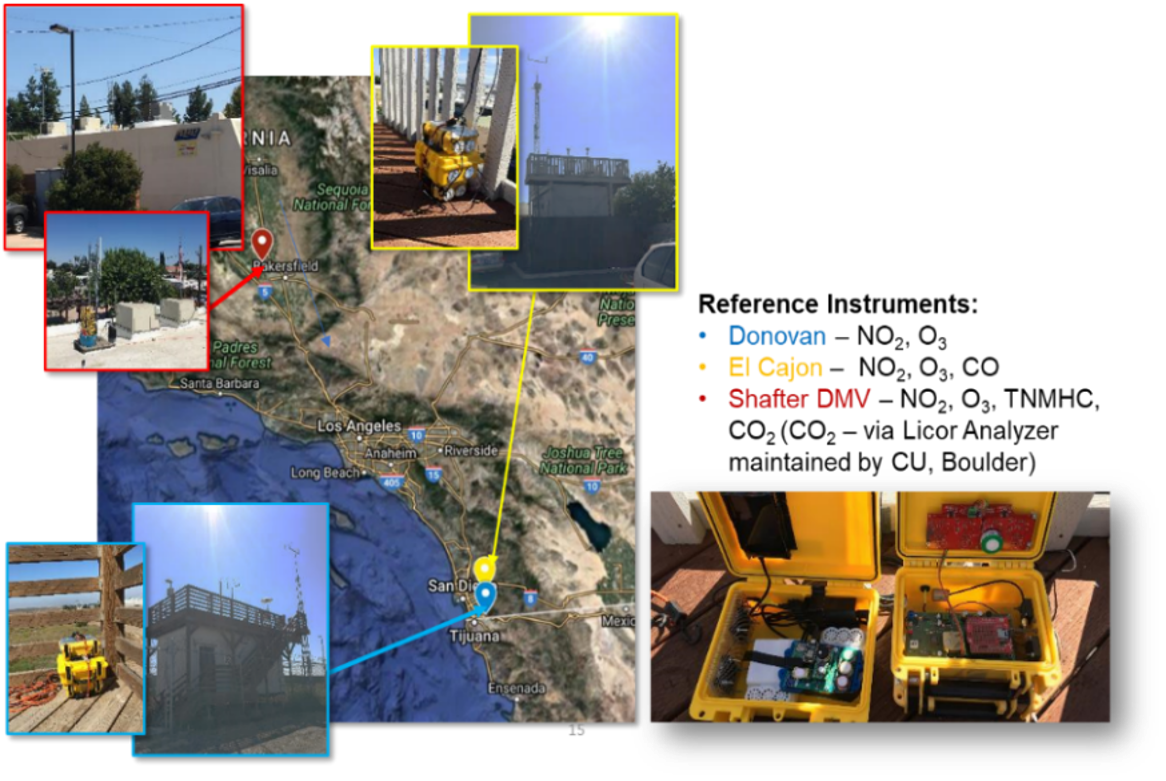
\includegraphics[width=0.75\textwidth]{writeup/img/MSdeployment.png}
\caption{Map and images of deployment locations}
\label{fig:img-label}
\end{figure}


\begin{table}[H]
\centering
\caption{Board locations for each round}
\begin{tabular}{l|llll}
                  & \textbf{Round 1} & \textbf{Round 2} & \textbf{Round 3} & \textbf{Round 4} \\ \hline
\textbf{Board 17} & N/A & El Cajon  & Shafter     &Donovan    \\
\textbf{Board 19} & Donovan & El Cajon       & Shafter       &Donovan   \\
\textbf{Board 21} & Donovan          & El Cajon         & Shafter        &Donovan  \\ \hline
\textbf{Board 11} & El Cajon         & Shafter          & Donovan        &El Cajon  \\
\textbf{Board 12} & El Cajon         & Shafter          & Donovan        &El Cajon  \\
\textbf{Board 13} & El Cajon         & Shafter          & Donovan         &El Cajon  \\ \hline
\textbf{Board 15} & Shafter          & Donovan          & El Cajon     &Shafter    \\
\textbf{Board 18} & Shafter          & Donovan          & El Cajon    &Shafter     \\
\textbf{Board 20} & N/A & Donovan          & El Cajon    &Shafter   
\end{tabular}
\label{tab:board-rotations}
\end{table}


\subsection{MetaSense Monitor Description} %Hardware, Sensor Signals, and Processing}

A low-cost air quality sensing platform was developed to interface with commercially available sensors [cite SPIE2017 paper, which has initial description]. The platform was designed to be mobile, modular, and extensible, enabling end users to configure the platform with sensors suited to their monitoring needs. It interfaces with the Particle Photon or Particle Electron [cite] platforms, which contain a 24 MHz ARM Cortex M3 microprocessor and a Wi-Fi or cellular module, respectively. In addition, a Bluetooth Low Energy module supports energy efficient communication with smartphones. The platform can interface with any sensor that communicates using standard communication protocols (i.e. analog, I2C, SPI, UART) and supports an input voltage of 3.3 V or 5.0 V. The platform can communicate results to nearby devices using BLE, or directly to the cloud using Wi-Fi, or 2G/3G cellular, depending on requirements.

Our configuration utilized electrochemical sensors for traditional air quality indicators (NO2, CO, Ox), nondispersive infrared sensors for CO2, photoionization detectors for volatile organic compounds (VOCs), and a variety of environmental sensors (temperature, humidity, barometric pressure). The electrochemical sensors (NO2: Alphasense NO2-A43F, Ox: Alphasense O3-A431, and CO: Alphasense CO-A4 are mounted to a companion analog front end (AFE) from Alphasense, which assists with voltage regulation and signal amplification. Electrochemical sensors offer a high level of accuracy at a low current consumption. Each sensing element has two electrodes which give analog outputs for the working electrode (WE) and auxiliary electrodes (AE). The difference in signals is approximately linear with respect to the ambient target gas concentration but have dependencies with temperature, humidity, barometric pressure, and cross-sensitivities with other gases. The electrochemical sensors generate an analog output, which is connected to a pair of ADCs (TI ADS6115) and converted into a digital representation of the measured voltage, which is later used as inputs for our machine learning models.

Modern low-cost electrochemical sensors offer a low cost and low power method to measure pollutants, but currently available sensors are not designed with air pollution monitoring as the primary focus: the overall sensing range is too wide and the noise levels are too high. For example, the commercially available sensors for NO2, Ox, and CO have a measurement range of 20, 20, and 500 ppm, respectively, which is significantly higher than the unhealthy range proposed by the United States Air Quality Index. Unhealthy levels for NO2 at 1-hour exposure range from 0.36 – 0.65 ppm, O3 at 1-hour exposure from 0.17 – 0.20 ppm, and CO at 8-hour exposure from 12.5 – 15.4 ppm. Along with the high range, the noise levels of the sensors make distinguishing whether air quality is Good or not difficult. Using the analog front end (AFE) offered by Alphasense, the noise levels for NO2, Ox, and CO have standard deviations of 7.5 ppb, 7.5 ppb, and 10 ppb, respectively. These standard deviations are large compared to the signal level for NO2 and Ox measurements, which range between 0 – 35 ppb and 12 – 60 ppb during the 6 month testing period, respectively.

The environmental sensors (MS5540C and SHT11) accurately measure temperature, humidity, and pressure and are important features for correcting the environmentally related offset in electrochemical sensor readings. The TE Connectivity MS5540C is a barometric pressure sensor capable of measuring across a 10 to 1100 mbar range with 0.1 mbar resolution. Across 0 C to 50 C, the sensor is accurate to within 1 mbar and has a typical drift of +/- 1 mbar per year. The Sensiron SHT11 is a relative humidity sensor capable of measuring across the full range of relative humidity (0 to 100\% RH) with a 0.05\% RH resolution. Both sensors come equipped with temperature sensors with +/-0.8 C and +/-0.4 C accuracy, respectively. The sensors stabilize to environmental changes in under 30 seconds, which is sufficiently fast to capture changes in the local environment.

In order to improve the robustness of the sensors to ambient conditions, the electronics were conformally coated with silicone and placed into a housing with the sensing elements. The housing prevents direct contact with the sensors by providing grates over the electrochemical sensors and a vent near the ambient environmental sensors for humidity, temperature, and barometric pressure. The system relies on passive diffusion of pollutants into the sensors due to the high power cost of active ventilation. The passive diffusion model is acceptable for the mobile sensor use case, though, because external movement of the sensor will cause a higher exchange rate of air into the enclosure. \todo{[do you want to show a picture of the case?]}  

For longer term static deployments, such as the presented case study that lasted 6 months, the sensors were placed into a more environmentally robust container. The container was a dry box, measuring 27.4 x 25.1 x 12.4 cm, that was machined to have two sets of two vents on opposing walls. Louvers were installed with two 5 V, 50 mm square axial fans expelling ambient air from one wall and two louvers allowing air to enter the opposite side. The configuration allowed the robust container to equilibrate with the local environment for accurate measurement. Due to the long timeframe of the deployment, a USB charging hub was installed into the container to power the fans, the air quality sensors, and either a BLU Android phone or Wi-Fi cellular hotspot. Each container could hold up to three air quality sensors with cases. The phones and hot spots were used to connect the sensors to the cloud; therefore, we could remotely monitor the sensors’ status in real-time, and perform preliminary data analysis and storage. All sensor nodes also had an SD card to record all measurements locally, increasing the reliability of data storage. 

\begin{figure}[H]
\centering
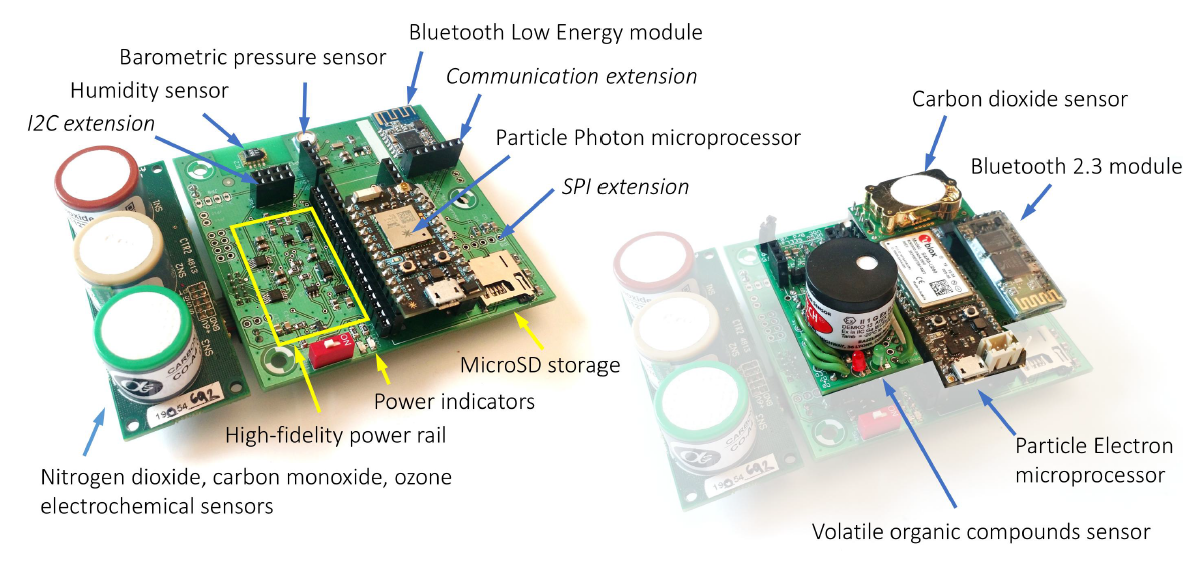
\includegraphics[width=0.75\textwidth]{writeup/img/metasense-platform}
\caption{labeled MetaSense board}
\label{fig:img-label}
\end{figure}

\subsection{MetaSense Software Infrastructure}

We developed the software infrastructure for the MetaSense sensing platform to support multiple usage scenarios. The firmware is configured to support four communication mediums. Every node can communicate via BLE and USB to a control program that can configure the platform and collect real-time data. In addition, the USB connection supports debugging the sensor behavior, charging the sensors, and updating the firmware. Depending on the hardware configuration, Photon or Electron, the MetaSense node can connect directly to the cloud via Wi-Fi or 3G cellular, respectively. These mediums enable over-the-air firmware updates. Each sensor is equipped with an SD card, allowing all readings to be stored locally for redundancy and for deployment situations where energy consumption is critical.

We developed two applications for Android smartphones that leverage the BLE connection of the MetaSense sensing platform. The first application, MetaSense Configurator App, lets users configure the hardware, adjusting aspects such as sensing frequency, the operation of specific sensors connected to the platform, and the communication mediums utilized. For example, CO2 and VOC sensor readings can be enabled or disabled by the configuration application. In another example, if the MetaSense sensing platform is being used as a mobile sensor tethered to a smartphone over BLE, users can disable Wi-Fi (or Cellular) radios to save power. The second application, the MetaSense App, collects data from the sensor via BLE and stores all readings in a database. The benefit of using this app is that each sensor reading is stamped with time and location information, supporting data analysis for mobile use cases. Moreover, users can read the current air quality information on their device, giving them immediate and personalized insight in their exposure to pollutants.

Finally, we developed a cloud backend in the Amazon cloud. Sensors can be configured to connect directly to this backend using Wi-Fi or 3G and transmit all readings to a database. We can then analyze the raw data either directly in the Amazon cloud by running our machine learning algorithms in virtual machines running in AWS or the data can be downloaded to be analyzed offline. While we use the Amazon cloud for our data collection and analysis, the Wi-Fi and 3G modules also connect to the Particle cloud, which provides a set of additional features including firmware updates, configuring and resetting the nodes, or monitoring their status remotely. These direct-to-cloud features are key to supporting the type of long-term deployments required for air quality sensor calibration such as the dataset collected for this paper.

\subsection{Quantification Techniques and Approaches}

Our sensors sample voltage values from each electrode roughly
once every 5 seconds. Although we have access to voltages from each electrode (active and working), we used the difference between the two (active minus working) as the representative voltage for each sensor. We found using them separately does not improve the quality of the models and this decision is also consistent with the methodology of \citet{Zimmerman2018}. We manually filtered out
anomalous values according to preset thresholds that search
for extreme voltage and temperature spikes (\todo{details can be found
in the appendix}). 
We obtained minute-averaged O3 and NO2 concentrations from the co-located EPA stations, and minute-averaged our own readings before joining
with the EPA data.
Over all three rounds of data collection, we obtained 1,200,000 measurements after minute-averaging. Each individual dataset was then split 80/20 into a train and test set.

Before using this data, we applied a series of simple filters which remove anomalous measurements. Specifically, we searched for temperature and voltage spikes which were outside the realm of reasonable values (for example 60 degrees Celsius), and removed the corresponding measurements.

Sensor calibration is the process of developing and training models to convert sensor voltages into usable pollutant concentrations. We formalize sensor calibration as a regression problem, with input features $x$ and $e$ representing board voltages (O3 voltage, NO2 voltage, CO voltage) and environmental factors (temperature, pressure, humidity) respectively for a total of 6 features. $y$ corresponds to pollutant concentrations (O3 ppb, NO2 ppb).

In regression, the goal is to develop a function $h_\theta(x, e)$
such that $h_\theta(x, e) \approx y$. This is often formalized as an optimization where we minimize error over a training dataset $\{x_n, e_n, y_n\}_{n = 1}^N$ according to a loss function $L(h_\theta(x, e), y)$, i.e. 
\begin{equation}
\theta^* = \argmin_\theta \frac{1}{N}\sum_{n = 1}^N L(h_\theta(x_n, e_n), y_n)
\end{equation}
Models trained in this way, however, assume that at test time, predictions
are made on data sampled from the training distribution. 
High-capacity models will often overfit the training distribution and when
predicting on out-of-distribution examples, will incur significant
error. Overfitting can be mitigated with regularization and by reducing
model capacity, but these tricks can only go so far if the test distribution
is drastically different from the train distribution.

The MetaSense project is concerned with deploying mobile, portable
sensors and thus we wish to train calibration models
that can generalize beyond the data obtained via co-location.
As previously described, we co-located MetaSense boards with EPA stations across three locations in California (El Cajon, Donovan, Shafter).
By training a calibration model on a training data restricted to some sites and testing on the other site, we measure how well particular models generalize to different locations.

We focus on four different baseline models, each trained using the Scikit-Learn Python package: 
\begin{enumerate}
    \item \textbf{Linear regression:} we assume the functional form $h(x) \triangleq w^T x + b$, and fit the parameters in closed form. We use no regularization or polynomial features.
    \item \textbf{Two-layer neural network:} we fit a two-hidden layer (200 wide) multilayer perceptron with rectified-linear unit activation functions and a final linear layer. We train this neural network using the Adam optimizer ($\beta_0 = 0.9, \beta_1 = 0.999$) and a learning rate of $10^{-3}$.
    \item \textbf{Four-layer neural network:} Same as two-layer neural network, but four hidden layers of width 200 instead of two.
    \item \textbf{Random forest:} We divide our data into five folds and train a random forest of size 100 on each fold, resulting in 500 trees. We aim to reproduce the strategy of \citet{Zimmerman2018} as closely as possible.
\end{enumerate}
With each of these four models, we performed a suite of identical benchmarks that measure various model transfer capabilities. We first initially split all datasets uniformly at random into train and test subsets, reserving 20\% of each board's data for testing.
In each benchmark, we progressively widen the training distribution by combining training data from more locations, while keeping the test set dataset from one location. We thus have four ``levels'' of benchmarks:
\begin{itemize}
    \item \textbf{Level 0:} train a model on one location and test on the same location
    \item \textbf{Level 1:} train a model on one location and test on another location
    \item \textbf{Level 2:} train a model on two locations and test on a third location 
    \item \textbf{Level 3:} train a model on three locations and test on one of the three
\end{itemize}
\begin{figure}
\begin{subfigure}{0.23\textwidth}
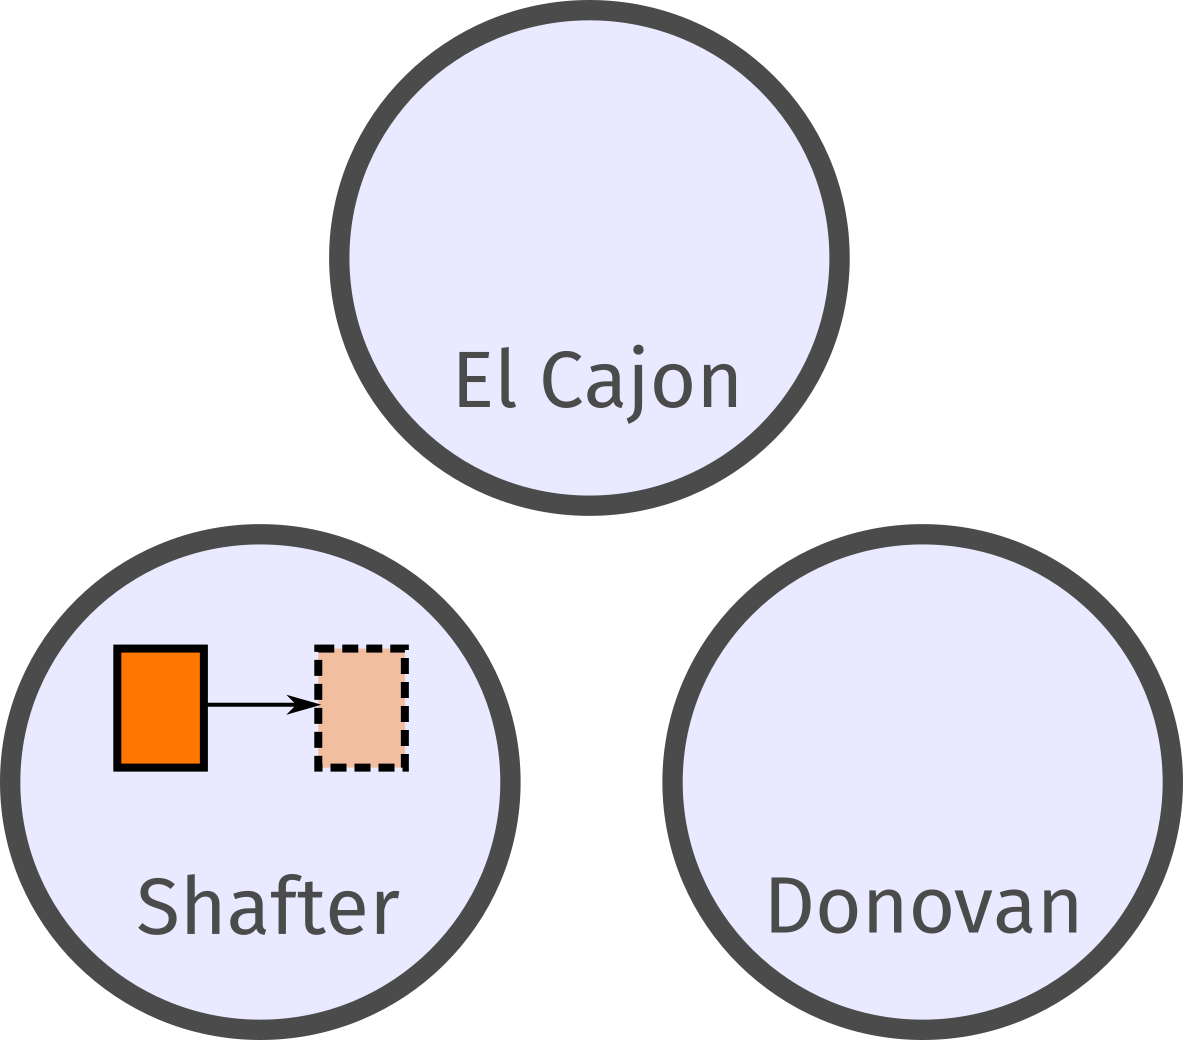
\includegraphics[width=\textwidth]{writeup/img/level0.png}
\caption{Level 0}
\end{subfigure}
~
\begin{subfigure}{0.23\textwidth}
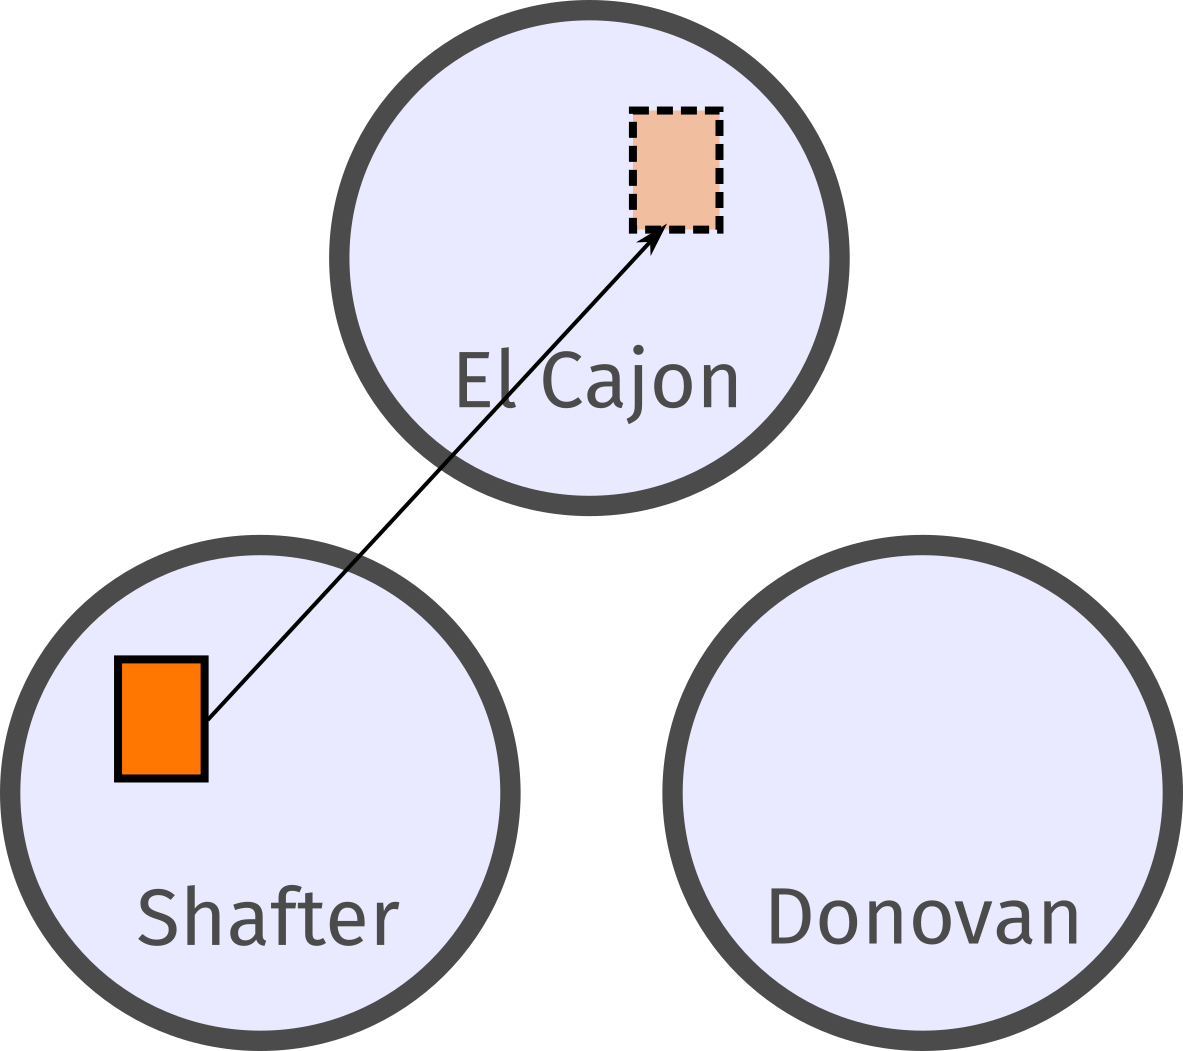
\includegraphics[width=\textwidth]{writeup/img/level1.png}
\caption{Level 1}
\end{subfigure}
~
\begin{subfigure}{0.23\textwidth}
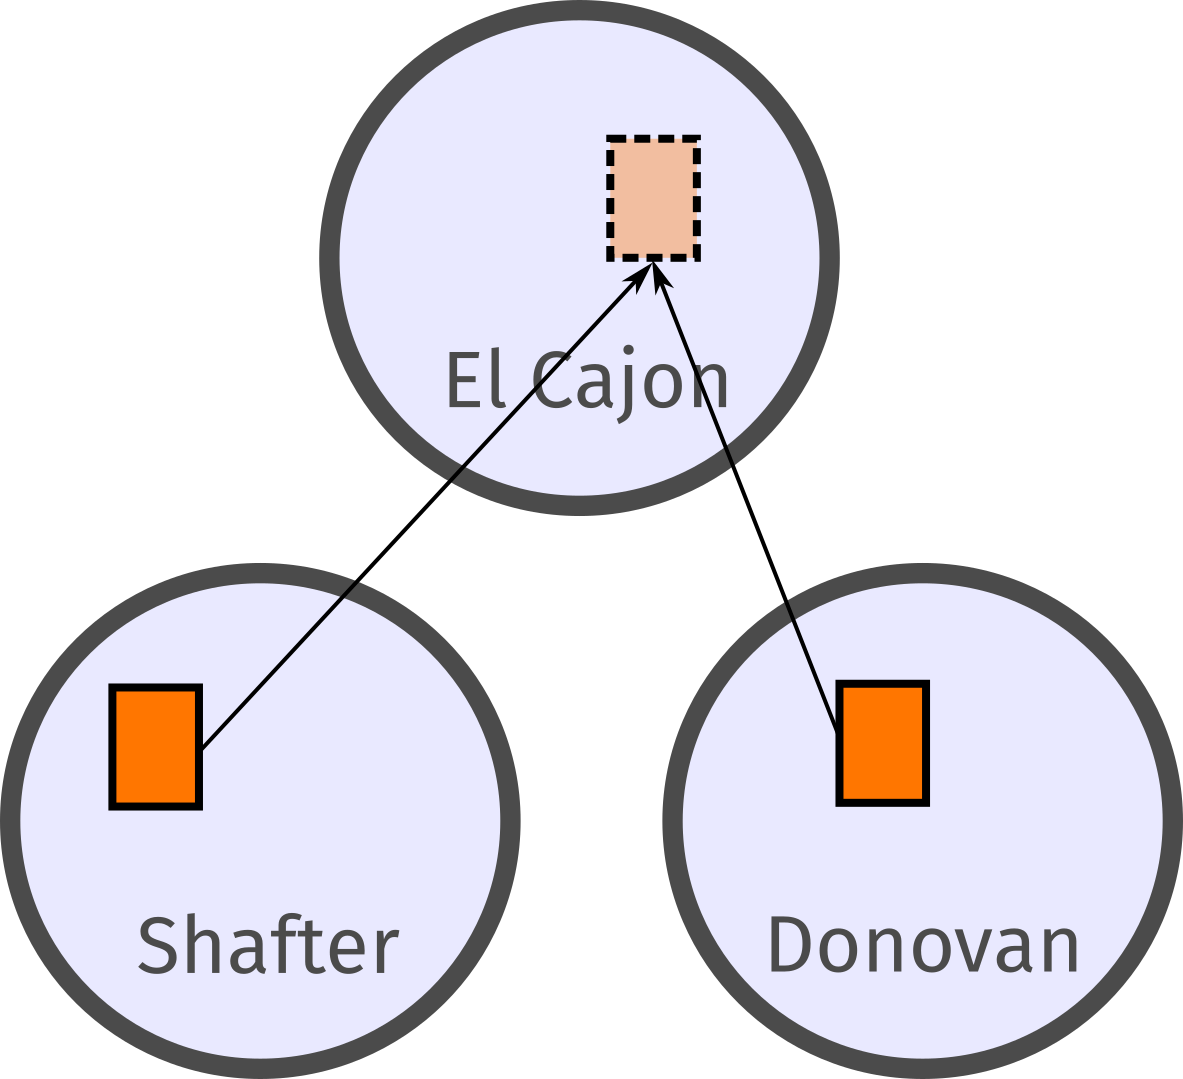
\includegraphics[width=\textwidth]{writeup/img/level2.png}
\caption{Level 2}
\end{subfigure}
~
\begin{subfigure}{0.23\textwidth}
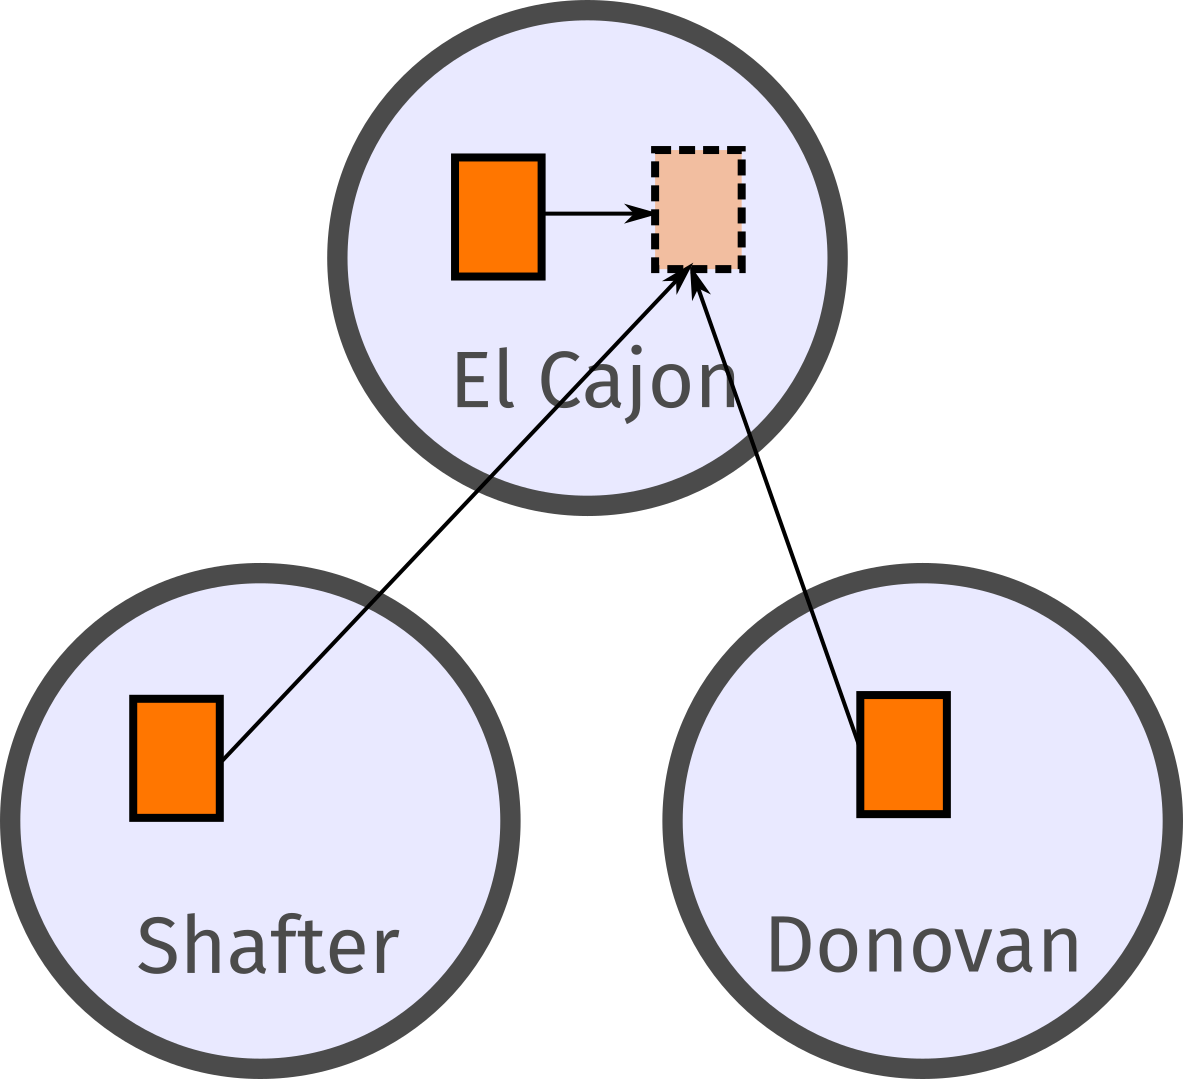
\includegraphics[width=\textwidth]{writeup/img/level3.png}
\caption{Level 3}
\end{subfigure}
\caption{Levels}
\end{figure}

Notably in Level 0 and Level 3 benchmarks, the train and test data distribution have explicit overlap, whereas in Level 1 and 2, there is no explicit overlap. 
The goal of this benchmark suite is to evaluate how expanding the data distribution can improve model transferability. We expect Level 0 performance to be the best, as the train and test distribution are identical. We also expect Level 1 performance to be the worst, as the training distribution is the narrowest and Level 3 to be close to Level 0 performance, due to the overlap in train and test distributions. 
Furthermore, we expect higher capacity models to overfit more to the training dataset, and thus have the biggest gap between Level 0 and Level 1. Thus, we expect linear regression to have more consistent performance across the benchmarks, followed by the 2-layer neural network, 4-layer neural network, and finally the random forest.

We ran each benchmark across all possible permutations of location and board,
measuring six metrics: root mean squared error (rMSE), centered root mean squared error (crMSE), mean absolute error (MAE), the coefficient of variation of mean absolute error (CvMAE), mean bias error (MBE), and coefficient of determination ($R^2$).
\iffalse
\begin{align*}
    \mathrm{MAE}(h(x), y) &= |h(x) - y| \\
    \mathrm{CvMAE}(h(x), y) &= \frac{1}{\textrm{Average conc. of pollutant}}|h(x) - y| \\
\end{align*}
\fi

\subsection{A Method for Improving Transferability}

A straightforward method to improve model transferability is collecting training data that more closely matches the test distribution.
This is reflected by the Level 2 and Level 3 results. The improvement from adding more data indicates that collecting data from a wider distribution can help in model transferability.
However, colocating sensors and moving them
several times can be expensive and takes more time to collect the training data.

Consider a collection of many boards. Previously, we would attribute each board $i$ with a calibration function $h_{\theta_i}(x)$, and fit this calibration function with colocated data.
We propose using a calibration function split into two distinct steps: first, we pass in pollutant sensor voltages $x$ into a sensor-specific model, $s_{\theta_i}(x)$ (a function parametrized by $\theta_i$, which outputs a fixed dimensional vector $u$. This intermediate representation $u$ is concatenated with environment data $e$ is then passed into a global calibration model $c_\phi([u | e])$. For a single board, our final calibration function is $c_\phi([s_{\theta_i}(x) | e])$.
In general, we use neural networks as the sensor-specific models and the global calibration models. We call this a ``Split-NN'' model. 

\begin{figure}
    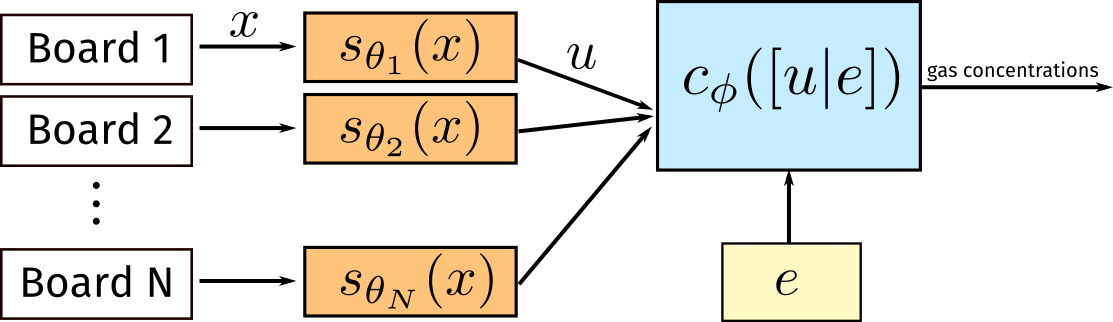
\includegraphics[width=0.8\textwidth]{writeup/img/split-model.png}
    \caption{}
\end{figure}

The split model can be trained efficiently with stochastic gradient descent. Specifically, we first collect $N$ datasets for each board $D_i = \{x^{(i)}, e^{(i)}, y^{(i)}\}_{i = 1}^N$. We ensure each of these datasets is the same size by sampling each with replacement to artificially match the largest dataset. We then pool the datasets together into one dataset from which we sample minibatches. Each sensor-specific model will be trained only on data collected by its sensor, but the global calibration model will be trained on all the data. Furthermore, sensor-specific models will be encouraged to output intermediate representations $u$ that are compatible with each other, since they are all fed into the same global model to produce pollutant levels.

Although training this neural network will take longer than training one for a single board, this method has some key advantages over conventional calibration techniques. 
The first is its ability to share information across both boards. 
Suppose Board A is trained on Location 1 and Board B is trained on Location 2. Pooling the datasets and using a shared model will encourage the global calibration model to predict well in both locations, and thus the calibration models for both boards will have information about the other locations in them, hopefully improving transferability.
The second is more efficient utilization of data. By pooling data and training jointly, we effectively multiply our data size by the number of boards we collect data for.

To evaluate this split model, we perform a Level 1 and Level 2 benchmark.
However, the Split-NN model is trained using data from every board whereas
the baseline models are only able to use data from one board at a time.


\subsection{Calibrating new boards}
Calibration at this point has been performed by colocating sensors with ground-truth sensors and training to match pollutant concentrations,
But, suppose we had a fleet of already low-cost sensors already deployed. 
A simpler method would be to colocate it with one of our $N$ calibrated boards and train a model to match the pollutant levels outputted by its calibration function. This risks compounding errors across models, however. 
The split model would enable calibrating new boards by colocating to match representation.
We propose calibrating the $N+1$-th sensor to match the intermediate representation outputted by colocated low-cost sensors. Specifically,
we train the $N + 1$ model to minimize $L(u_N, u_{N + 1})$, or
the loss between the the two board's intermediary outputs.
These intermediate representations are meant to be robust to changes in location so training to match these representation will hopefully result in a robust calibration model. We analyze this potential calibration technique by holding out a board from our datasets and training a split model. We then simulate calibrating the held out board by training a sensor model to match the representations produced by another board it was colocated with. We then use this new sensor model with the global calibration function to produce pollutant values. 

The Split-NN offers a novel method to calibrate new boards.
Suppose we have a set of $N$ calibrated boards and are presented with an uncalibrated $N + 1$-th board. The safest way to calibrate this new board would is always to colocate it with a ground-truth sensor and train a model. 
This requirement, however, is potentially restrictive and expensive, as it
necessitates deploying the sensor by an EPA or other reliable sensor.
On the other hand, colocating with another low cost sensor is simple
and cheap, but risks
compounding the noise and error that already exist.

\section{Results \& Discussion}

\subsection{Robustness of Different Sensor Quantification Techniques Across New Locations}

We observe that on average, as model capacity increases, Level 0 error decreases. This is consistent across both NO2 and O3 prediction and reflects the ability of the model to fit the train distribution. Level 1 and 2 benchmarks reflect the ability of a model to generalize to a distribution it hasn't seen before and we see that in these benchmarks, errors are much higher and the gaps between models is smaller.
Furthermore, Level 2 error is lower than Level 1 error. By adding data from another site, effectively widening the training data distribution, the models become more robust to the unseen test distribution. Level 3 performance aligns closely with Level 0 performance, which is to be expected, since in both cases
the train distribution matches the test distribution.

Across baselines, we observe that on average, linear regression has the highest error on all the benchmarks. However, its error across the Level benchmarks more consistent than the other models, suggesting that low-capacity linear regression are more robust to transfer. On the other hand, random forests (RFs) have on average the lowest error, but have far more inconsistent results across the Levels. The results indicate a tradeoff between model capacity and robustness to transfer, consistent with our intuitions about model overfitting and generalization. Neural networks lie in between linear regression and random forests, and offer a tradeoff between low error and consistent error. 

These results suggest good practices when deploying models. Training a complex RF calibration model will likely result in very low error at a colocated site, but could incur significant error at a different site. Although their predictions at a new site will have lower error than linear regression, the error they have at the train site will likely not be representative of their error in practice. A linear model, on the other hand, despite not predicting as well at the train site, will not have significantly more error at test time.

\begin{figure}[H]
\centering
\begin{subfigure}{0.45\textwidth}
\includegraphics[width=\textwidth]{\baselinedir/NO2" "MAE_test.png}
\caption{NO2}
\end{subfigure}
\begin{subfigure}{0.45\textwidth}
\includegraphics[width=\textwidth]{\baselinedir/O3" "MAE_test.png}
\caption{O3}
\end{subfigure}
\caption{}
\label{fig:results-linear}
\end{figure}

\iffalse

\begin{itemize}
    \item  \emph{Current techniques assume that the conditions of sensor use match those of calibration.  How reasonable are these assumptions in practice?}
    \begin{itemize}
        \item Summarize the results of training on one location and testing on the others, compare the results across MLR, NN, and RF 
        \item Discuss the implications of these results, what does it mean for groups that are calibrating sensors in one location in a city and then moving them to new locations? Or groups calibrating in one city and deploying in another city? Is the drop in performance worse for moving sensors to a new city versus a new location in the same city (this could be valuable information for other researchers and regulatory agencies) Also, out of the quantification techniques tested (MLR, NN, RF) which would be recommended for different situations?
    \end{itemize}
    \item When they fail, what are the underlying causes of those failures?  (E.g., variance in humidity, temperature, barometric pressure, or background pollutants.)
    \begin{itemize}
        \item When we have a drop in performance is there still any valuable information in the data (i.e., are the trends still there, is it simply a shift causing the poorer performance?) -> a time series of training data from one San Diego site and that same model tested at the other San Diego site and the Shafter site could help us figure this out. (plot model tested on other site)
        \item Can these drops in performance be attributed to mainly a change in environmental and pollutant distributions between sites OR do different overall/background compositions at sites (based on environmental differences, different sources near and far, etc.) play a large role.
        \item different data distribution
        \item overfitting to environment experiments
        \item include data about RF leaves
    \end{itemize}
\end{itemize}
\fi

To better understand how model performance degrades, we produce
target plots, which visualize the tradeoff between error and bias.
The target plots indicate that model bias becomes a much more significant issue
after moving locations. In \autoref{fig:target-plots-models}, we observe
that Level 0 and 3 results have relatively low bias with respect
to error, but Level 1 and 2 have an explosive increase
in bias. The increase in bias is more pronounced in the higher capacity models, especially random forests. \autoref{fig:target-plots-models} indicates that despite the higher capacity models showing better error and bias in a Level 0 benchmark, the models have very similar error-bias tradeoffs in a Level 1 benchmark, indicating that even a high capacity model cannot avoid this performance degradation.

The large increase in bias suggest that perhaps some sort of correction to a model may go a long way in improving model performance after transfer. This result motivates the use of the split neural network architecture, which has a model-specific correction stage that enables learning (hopefully) unbiased representations of sensor measurements.

\begin{figure}[H]
\centering
\begin{subfigure}{0.45\textwidth}
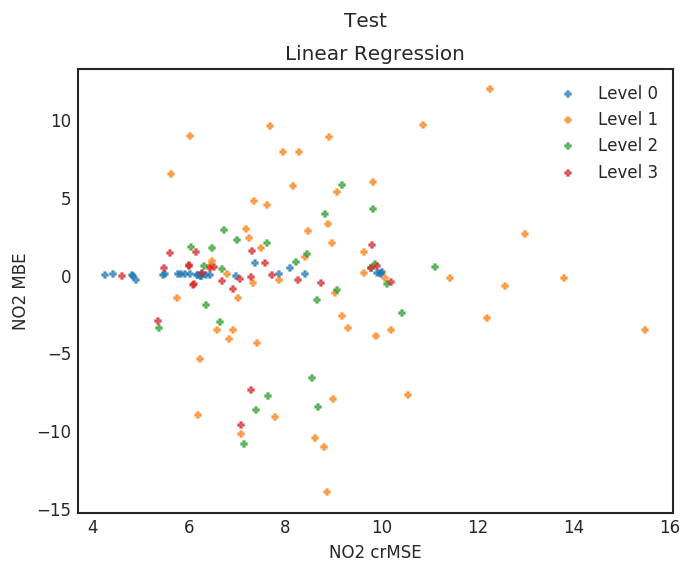
\includegraphics[width=\textwidth]{\baselinedir/NO2_linear_test_target.png}
\caption{Linear Regression (NO2)}
\end{subfigure}
\begin{subfigure}{0.45\textwidth}
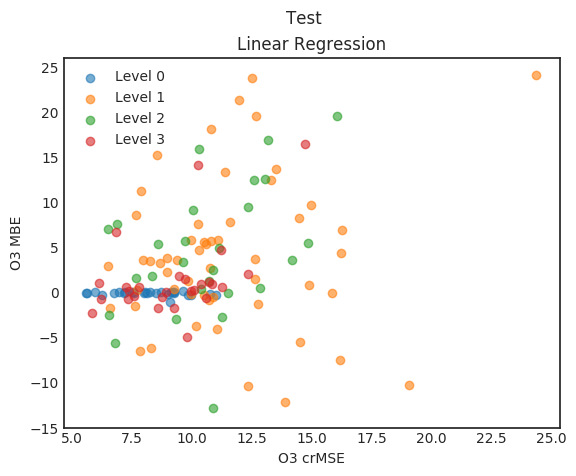
\includegraphics[width=\textwidth]{\baselinedir/O3_linear_test_target.png}
\caption{Random Forest (O3)}
\end{subfigure}
\begin{subfigure}{0.45\textwidth}
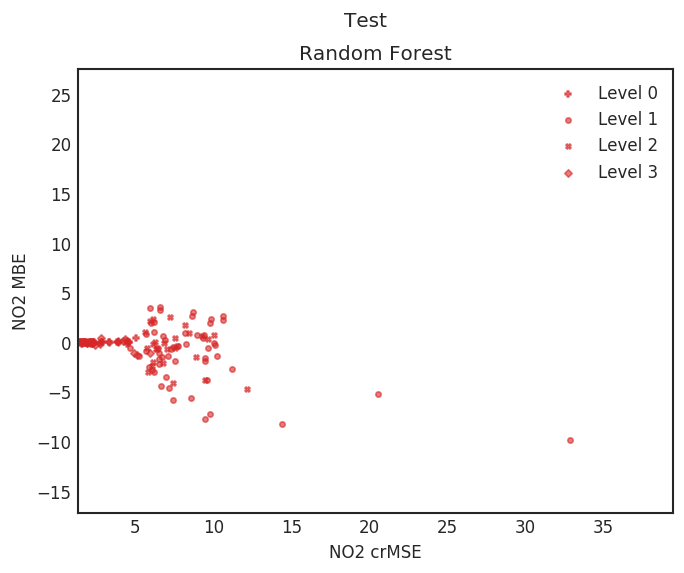
\includegraphics[width=\textwidth]{\baselinedir/NO2_subu_test_target.png}
\caption{Random Forest (NO2)}
\end{subfigure}
\begin{subfigure}{0.45\textwidth}
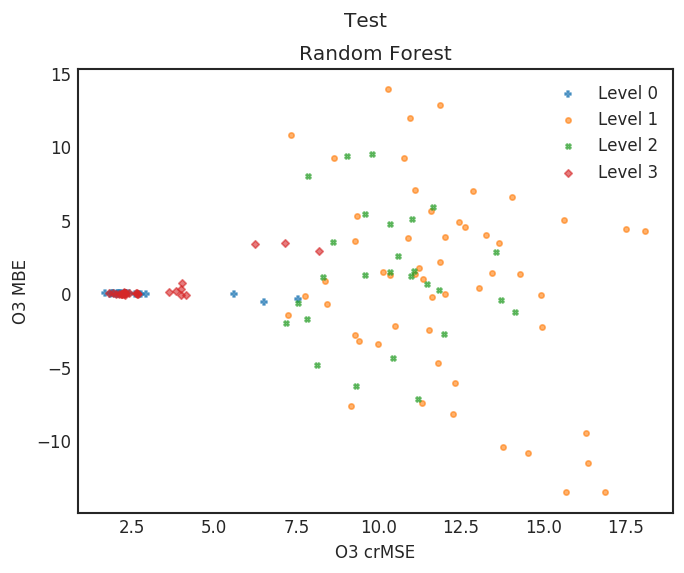
\includegraphics[width=\textwidth]{\baselinedir/O3_subu_test_target.png}
\caption{Random Forest (O3)}
\end{subfigure}
\caption{}
\label{fig:target-plots-models}
\end{figure}

\begin{figure}[H]
\centering
\begin{subfigure}{0.45\textwidth}
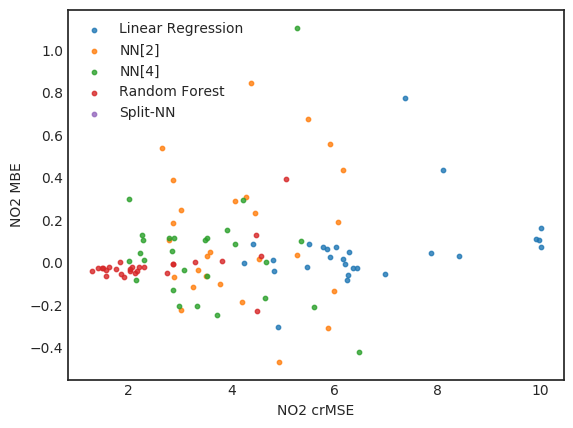
\includegraphics[width=\textwidth]{\baselinedir/NO2_level0_test_target.png}
\caption{Level 0 (NO2)}
\end{subfigure}
\begin{subfigure}{0.45\textwidth}
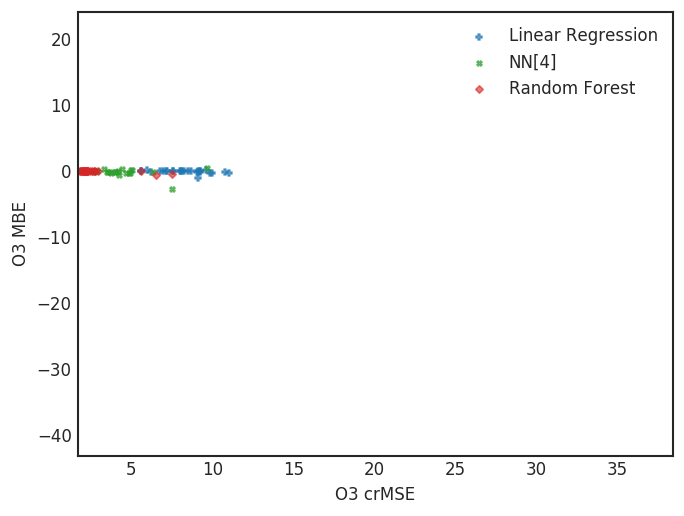
\includegraphics[width=\textwidth]{\baselinedir/O3_level0_test_target.png}
\caption{Level 0 (O3)}
\end{subfigure}
\begin{subfigure}{0.45\textwidth}
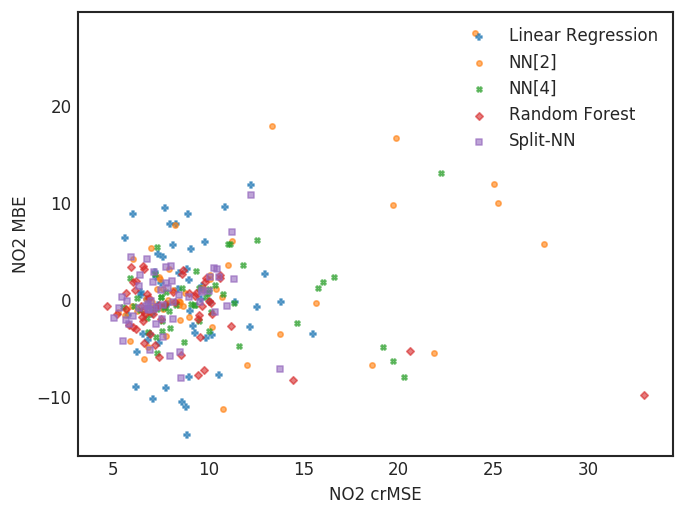
\includegraphics[width=\textwidth]{\baselinedir/NO2_level1_test_target.png}
\caption{Level 1 (NO2)}
\end{subfigure}
\begin{subfigure}{0.45\textwidth}
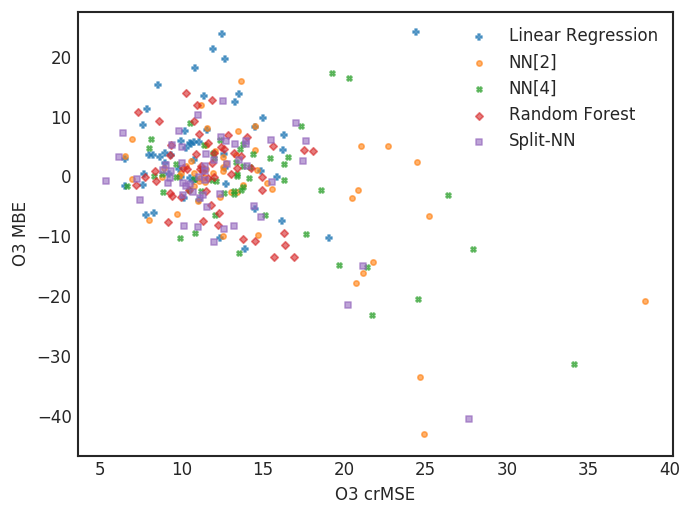
\includegraphics[width=\textwidth]{\baselinedir/O3_level1_test_target.png}
\caption{Level 1(O3)}
\end{subfigure}
\caption{}
\label{fig:target-plots-levels}
\end{figure}


In general, however, we observe that model performance degrades non-trivially
when moved to different locations. This decrease in performance could result in overconfidence in a sensor's readings, potentially affecting downstream decisions. We briefly analyze the properties of our data that could result in overfitting.
\todo{(perhaps add something like: the model is overfitting to ambient environmental conditions and not the sensor reading. Many pollutants change with the diurnal cycle of the earth (eg. NO2 turning into O3 only when there is UV light, so NO2 is bigger at night, which is typically cooler and more/less humidity).)}.
We first investigate how data distributions across sites and times differ. Over each location and round, pollutant values can be highly variable. This is reflected, for example, in \autoref{fig:no2-rounds} where Shafter has higher values of NO2 in Round 1 and 2 but lower in Round 3. Furthermore, in \autoref{fig:o3-rounds}, the distribution of O3 changes remarkably across round and location.
Similarly, temperature and humidity change significantly across location and round, which can be seen in \autoref{fig:temperature-rounds} and \autoref{fig:humidity-rounds}.

\iffalse
To determine whether models overfit to a particular feature, we evaluate their train and test performance on the datasets with and without the feature. We found that (models overfit to temperature) \todo{fill in this section}.
\fi

\begin{figure}[H]
\centering
\begin{subfigure}{0.45\textwidth}
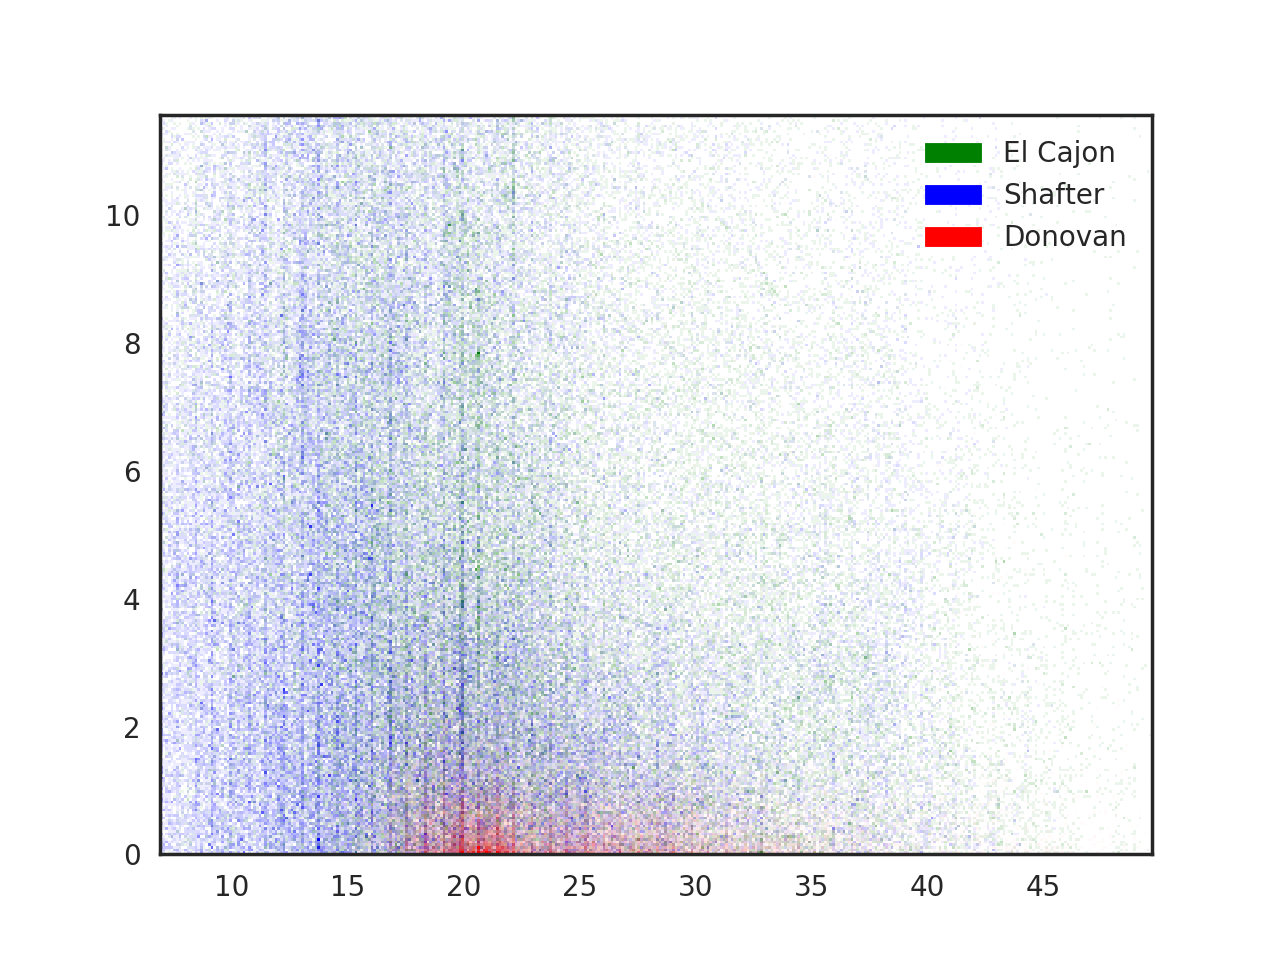
\includegraphics[width=\textwidth]{\baselinedir/linear/error_density_temperature_donovan_NO2.png}
\caption{Temperature - Linear Regression (NO2, Donovan)}
\end{subfigure}
\begin{subfigure}{0.45\textwidth}
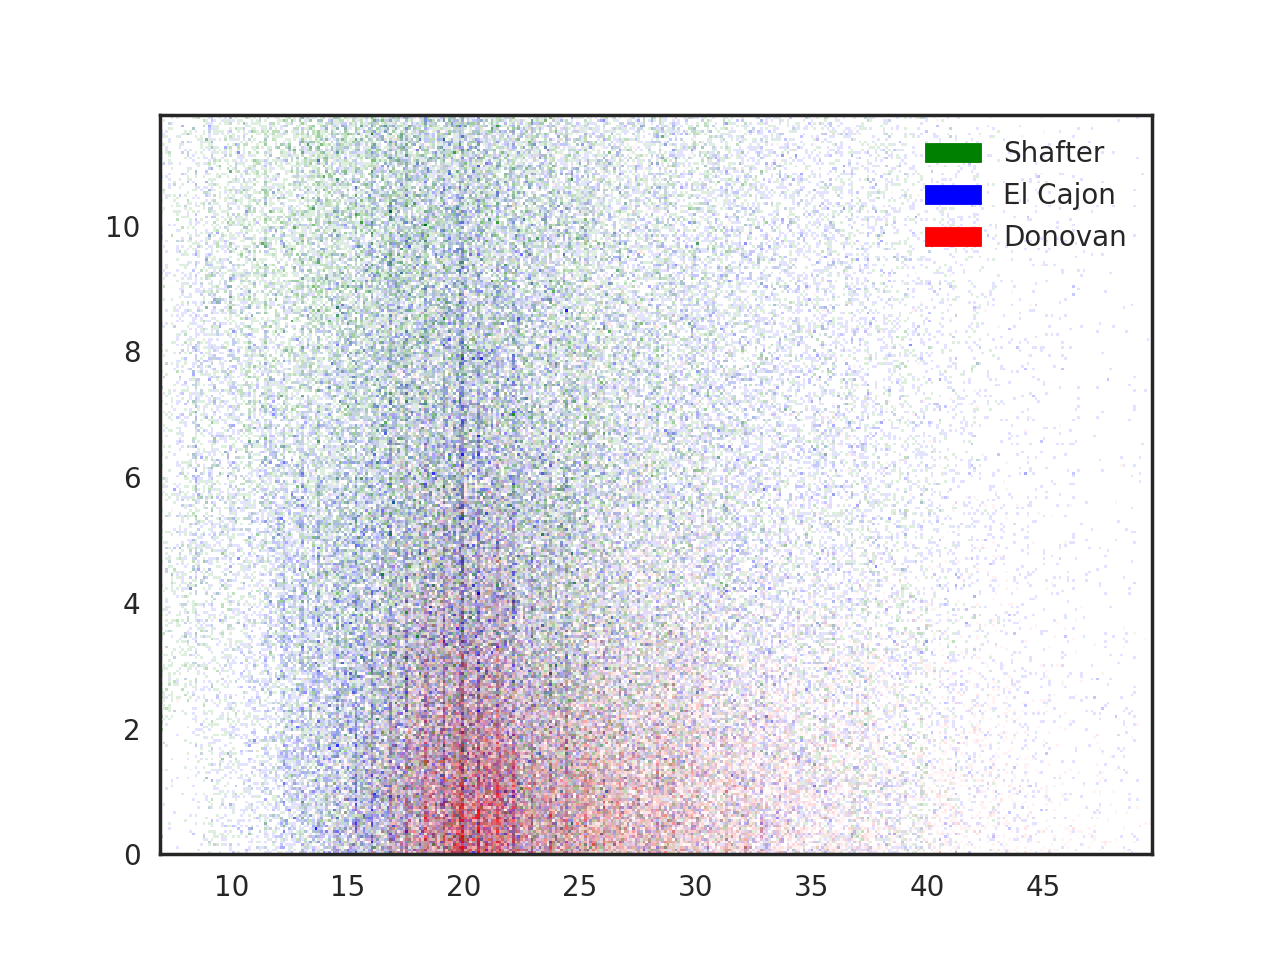
\includegraphics[width=\textwidth]{\baselinedir/linear/error_density_temperature_donovan_O3.png}
\caption{Temperature - Linear Regression (O3, Donovan)}
\end{subfigure}
\caption{}
\label{fig:target-plots-models}
\end{figure}

\subsection{Approaches to Increase the Robustness of Calibrations}

In this section, we evaluate the Split-NN's utility for calibration.
We evaluate the Split-NN by performing Level 1 and Level 2 benchmarks, comparing to the baselines. The Split-NN is trained by
holding out particular locations but training on all boards on the 
remaining locations.
In these results, our model on average has lower MAE and CvMAE in Level 1 and Level 2 benchmarks for the random forest model. We examine this further
by taking the difference in errors between the same permutations 
in each benchmark. We find on average, our models have $0.374$ ppb less MAE  
for NO2 prediction and $0.436$ ppb less MAE for O3 prediction.
We also find these results consistent across the other metrics,
a promising indication that pooling data across boards offers
improvements, even if marginal.

\begin{figure}[H]
\begin{subfigure}{0.49\textwidth}
\includegraphics[width=\textwidth]{\splitdir/locations/NO2" "MAE.png}
\caption{NO2 MAE}
\end{subfigure}
\begin{subfigure}{0.49\textwidth}
\includegraphics[width=\textwidth]{\splitdir/locations/O3" "MAE.png}
\caption{O3 MAE}
\end{subfigure}
\begin{subfigure}{0.49\textwidth}
\includegraphics[width=\textwidth]{\splitdir/locations/NO2" "MAE-diff.png}
\caption{NO2 MAE difference}
\end{subfigure}
\begin{subfigure}{0.49\textwidth}
\includegraphics[width=\textwidth]{\splitdir/locations/O3" "MAE-diff.png}
\caption{O3 MAE difference}
\end{subfigure}
\caption{Comparison of errors of Split NN and RFs.}
\label{fig:split-comparison}
\end{figure}



\begin{figure}
    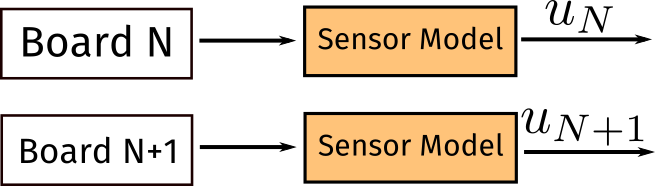
\includegraphics[width=0.5\textwidth]{writeup/img/split-calibration}
    \caption{Calibrating a new board $N + 1$}
\end{figure}

\iffalse

\begin{itemize}
    \item Given these failure modes, how can data collection and model training be improved to overcome these failures?
      \begin{itemize}
          \item Collect data from multiple sites and either:
          \begin{itemize}
            \item Average models over multiple diverse locations 
            \item Pool all the data together and build a single model
          \end{itemize}
      \end{itemize}
    \item Given that it is typical to calibrate many sensors, how should calibration data from multiple sensors be employed to achieve the best results?
      \begin{itemize}
          \item Collect data from all sensors to be calibrated and build a single shared model
      \end{itemize}
    \item Finally, (how) can multiple-site techniques and multiple-sensor techniques be combined?
      \begin{itemize}
         \item Neural networks work, and random forest doesn’t, because they are more modular (differentiability)
      \end{itemize}
    \item Can a new sensor can be affordably and accurately calibrated without having to repeat the whole data collection cycle?
      \begin{itemize}
          \item Simple colocation with a single sensor
          \item Match new sensor to the global model through co-location with one of the calibrated sensors
      \end{itemize}
\end{itemize}
\fi

\iffalse
\subsection{Additional Observations and Recommendations}

\begin{itemize}
    \item \todo{Model size}
    \item \todo{Calibrate over a lot of sites}
    \item If one doesn't have access to multiple sites (or only two instead of three), can multiple locations be approximated by just training longer at one site? \emph{maybe}
    \item Translate what we've learned into practical advice for an average citizen scientist group - how can they use this information to improve their work and given typical real-world constraints where can they focus their efforts in order to get the best data quality possible (maybe this section should include a list of hypothetical) 
\end{itemize}
\fi

\section{Conclusion}

A rotating deployment strategy enables benchmarking the transferability of models. We found that overfitting is a concern, especially when transferring high capacity models trained with limited data. Level 2 benchmarks indicate that widening the data distribution is a good strategy to make models robust to transfer and we introduce a novel split-neural network strategy that increases effective data size, increasing the robustness of the model to transfer.

We hope to extend this work to answer a few key questions that we believe are relevant to the future of low-cost sensor calibration. 
We hope to determine the effect of temporal resolution on accuracy. Currently, sensors are sampled every five seconds, but ground truth data only exists at the minute level. By averaging our own sensor measurements every minute, we discard data that could potentially be relevant for calibration. We believe recent advances in recurrent neural networks for sequence prediction can help leverage the high-resolution data for robust prediction. In this vein, we also hope determine the effect of mobility on calibration functions. In this paper, we studied the effect of moving sensors from one static location to another but a potent application of low-cost sensing is mobile sensors, perhaps attached to a person or vehicle. A dynamic data distribution is a challenge that we hope our methods can generalize to.

\iffalse
\begin{itemize}
    \item What is the tradeoff between resolution and accuracy, if any. 
    \item Mobility causes fast changes. Brief high exposures could be harmful.
    \item Our sensors change slowly, taking up to 30 seconds to respond to a change in signal
    \item Noise, Drift?
\end{itemize}
\fi

\bibliographystyle{copernicus}
\bibliography{main.bib}


%%%%%%%%%%%%%%%%%%%%%%%%%%%%%%%%%%%%%%%%%%%%%
%%%%%%%%%%%%%%%%%%%%%%%%%%%%%%%%%%%%%%%%%%%%%

\appendix
\setcounter{table}{0}

\section{Data}

We have been collecting data from nine boards
from three sites in southern California.
\begin{enumerate}
    \item El Cajon
    \item Donovan
    \item Shafter
\end{enumerate}
We have split up the boards and rotated the boards
between locations every two weeks (see \autoref{tab:board-rotations}).

We do not have CO data for Shafter and Donovan, so we will focus only on
O3 and NO2.

\section{Distributions}
In this section, we describe
and visualize the distributions
of various values in the data.

\subsection{Environment}

\begin{figure}[H]
\centering
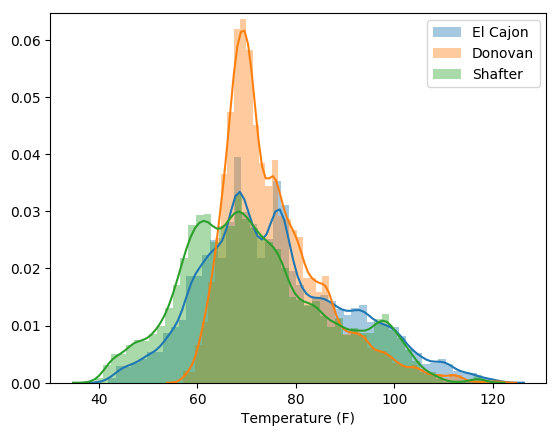
\includegraphics[width=0.5\textwidth]{results/distributions/temperature.png}
\caption{Temperature distribution based on
location}
\label{fig:temperature}
\end{figure}

\begin{figure}[H]
\centering
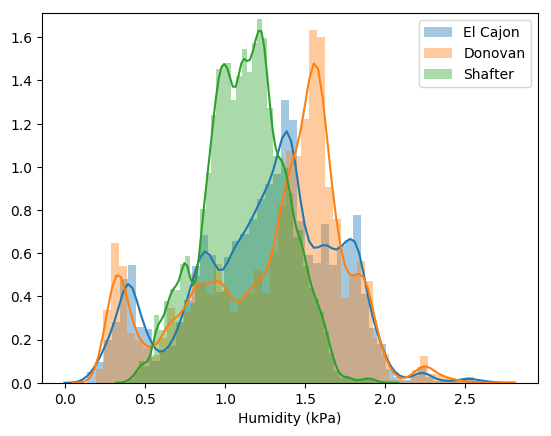
\includegraphics[width=0.5\textwidth]{results/distributions/humidity.png}
\caption{Absolute humidity distribution based on
location}
\label{fig:humidity}
\end{figure}

\begin{figure}[H]
\centering
\begin{subfigure}{0.32\textwidth}
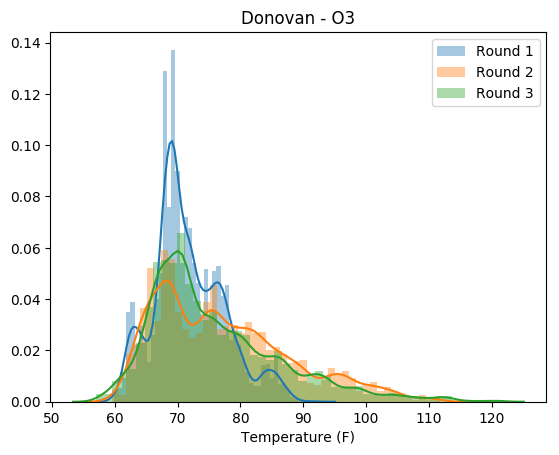
\includegraphics[width=\textwidth]{results/distributions/location_donovan_temperature.png}
\caption{Donovan}
\end{subfigure}
\begin{subfigure}{0.32\textwidth}
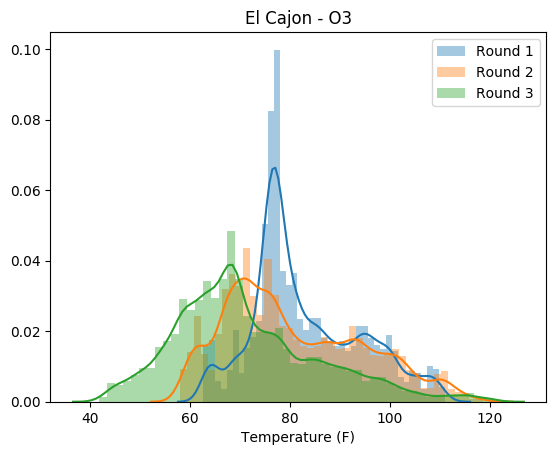
\includegraphics[width=\textwidth]{results/distributions/location_elcajon_temperature.png}
\caption{El Cajon}
\end{subfigure}
\begin{subfigure}{0.32\textwidth}
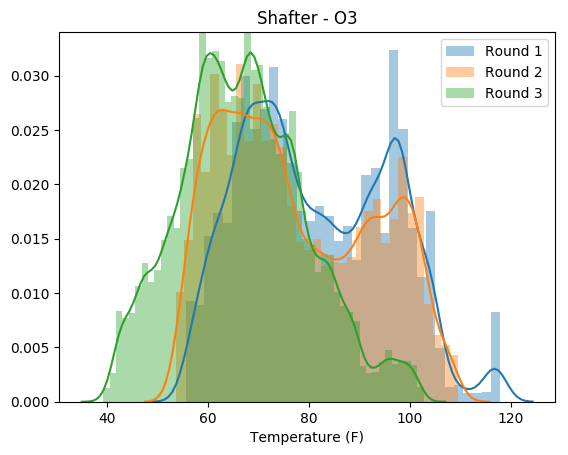
\includegraphics[width=\textwidth]{results/distributions/location_shafter_temperature.png}
\caption{Shafter}
\end{subfigure}
\caption{Temperature at locations}
\label{fig:temperature-locations}
\end{figure}

\begin{figure}[H]
\centering
\begin{subfigure}{0.32\textwidth}
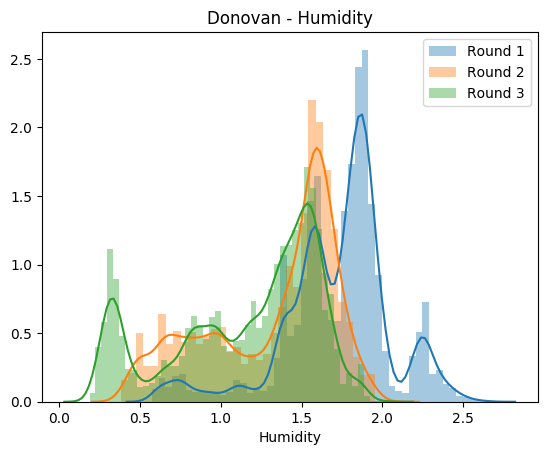
\includegraphics[width=\textwidth]{results/distributions/location_donovan_humidity.png}
\caption{Donovan}
\end{subfigure}
\begin{subfigure}{0.32\textwidth}
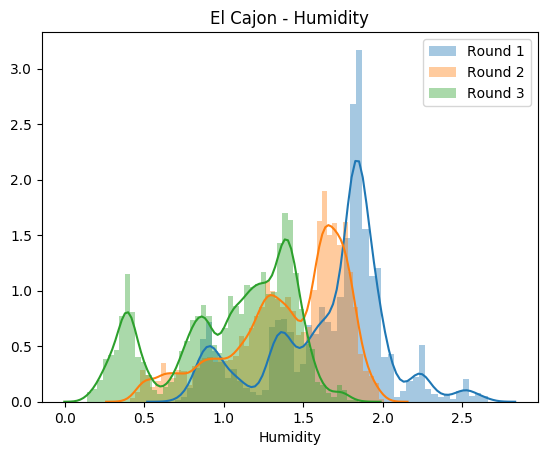
\includegraphics[width=\textwidth]{results/distributions/location_elcajon_humidity.png}
\caption{El Cajon}
\end{subfigure}
\begin{subfigure}{0.32\textwidth}
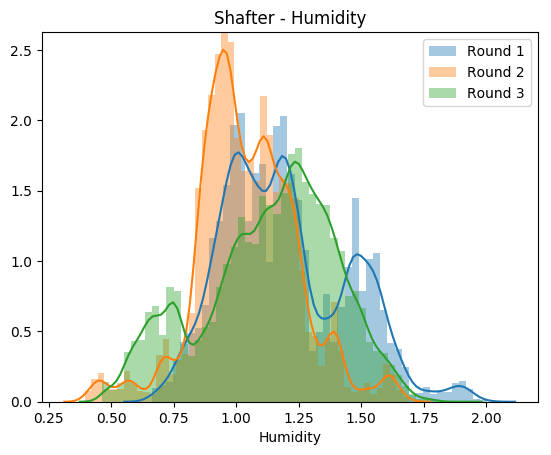
\includegraphics[width=\textwidth]{results/distributions/location_shafter_humidity.png}
\caption{Shafter}
\end{subfigure}
\caption{Absolute humidity at locations}
\label{fig:humidity-locations}
\end{figure}

\begin{figure}[H]
\centering
\begin{subfigure}{0.32\textwidth}
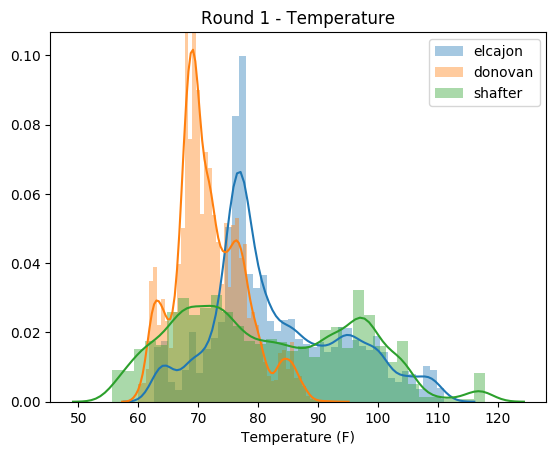
\includegraphics[width=\textwidth]{results/distributions/round1_temperature.png}
\caption{Round 1}
\end{subfigure}
\begin{subfigure}{0.32\textwidth}
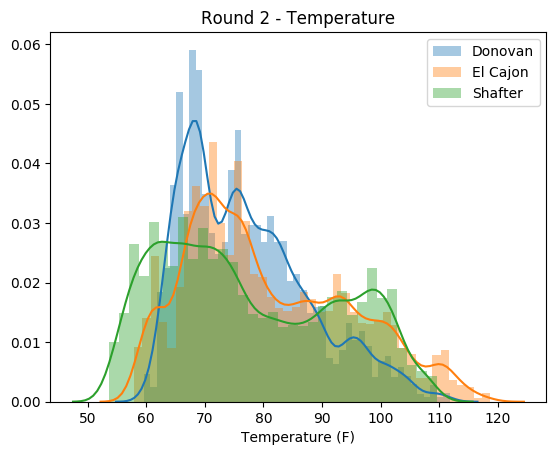
\includegraphics[width=\textwidth]{results/distributions/round2_temperature.png}
\caption{Round 2}
\end{subfigure}
\begin{subfigure}{0.32\textwidth}
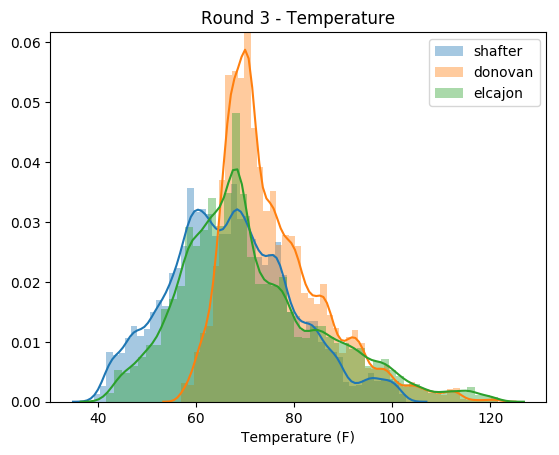
\includegraphics[width=\textwidth]{results/distributions/round3_temperature.png}
\caption{Round 3}
\end{subfigure}
\caption{Temperature over rounds}
\label{fig:temperature-rounds}
\end{figure}

\begin{figure}[H]
\centering
\begin{subfigure}{0.32\textwidth}
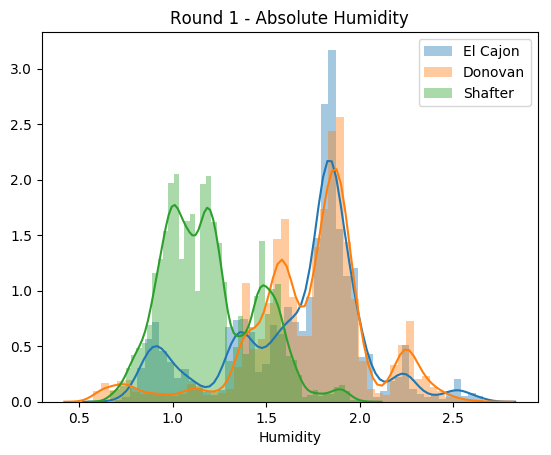
\includegraphics[width=\textwidth]{results/distributions/round1_humidity.png}
\caption{Round 1}
\end{subfigure}
\begin{subfigure}{0.32\textwidth}
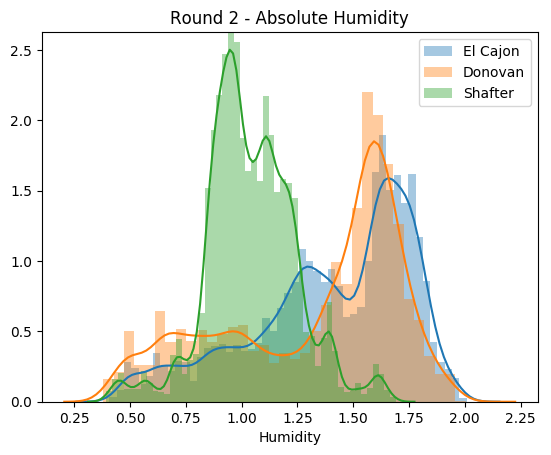
\includegraphics[width=\textwidth]{results/distributions/round2_humidity.png}
\caption{Round 2}
\end{subfigure}
\begin{subfigure}{0.32\textwidth}
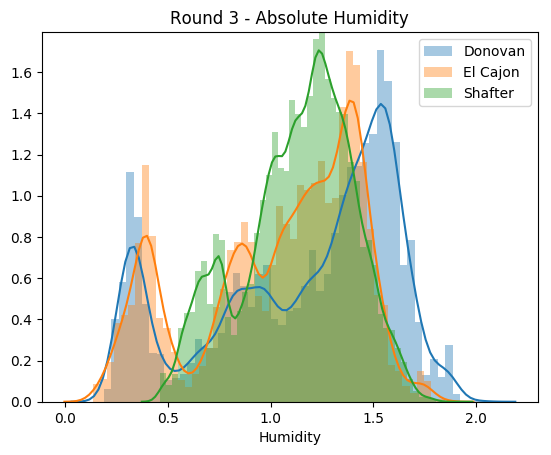
\includegraphics[width=\textwidth]{results/distributions/round3_humidity.png}
\caption{Round 3}
\end{subfigure}
\caption{Humidity over rounds}
\label{fig:humidity-rounds}
\end{figure}


\subsection{Pollutant values}

\begin{figure}[H]
\centering
\begin{subfigure}{0.32\textwidth}
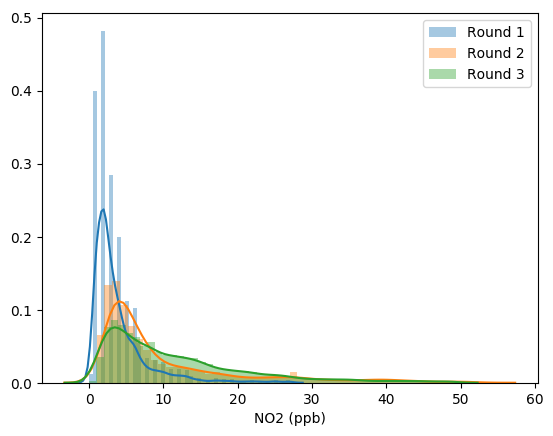
\includegraphics[width=\textwidth]{results/distributions/location_donovan_no2.png}
\caption{Donovan}
\end{subfigure}
\begin{subfigure}{0.32\textwidth}
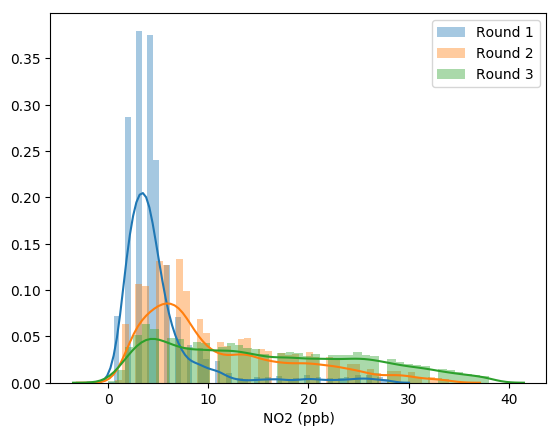
\includegraphics[width=\textwidth]{results/distributions/location_elcajon_no2.png}
\caption{El Cajon}
\end{subfigure}
\begin{subfigure}{0.32\textwidth}
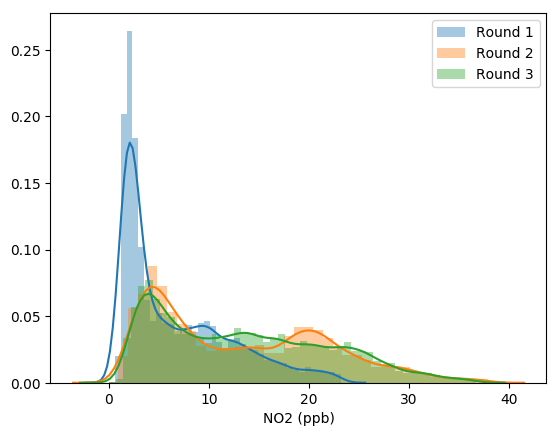
\includegraphics[width=\textwidth]{results/distributions/location_shafter_no2.png}
\caption{Shafter}
\end{subfigure}
\caption{NO2 at locations}
\label{fig:no2-locations}
\end{figure}

\begin{figure}[H]
\centering
\begin{subfigure}{0.32\textwidth}
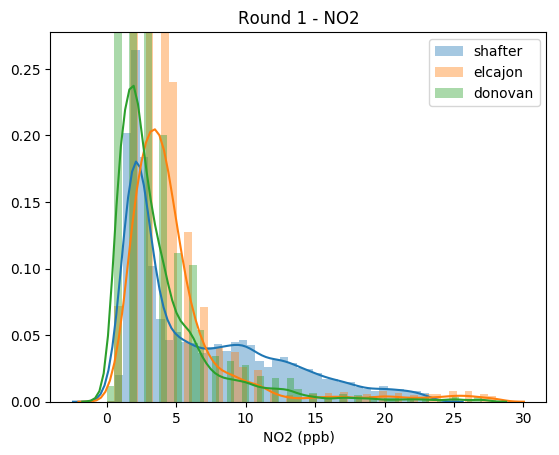
\includegraphics[width=\textwidth]{results/distributions/round1_no2.png}
\caption{Round 1}
\end{subfigure}
\begin{subfigure}{0.32\textwidth}
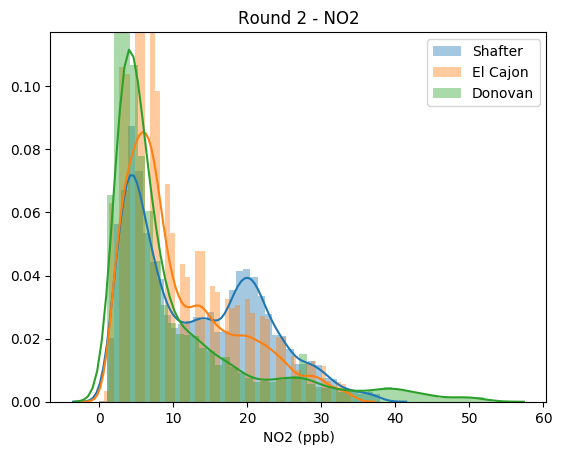
\includegraphics[width=\textwidth]{results/distributions/round2_no2.png}
\caption{Round 2}
\end{subfigure}
\begin{subfigure}{0.32\textwidth}
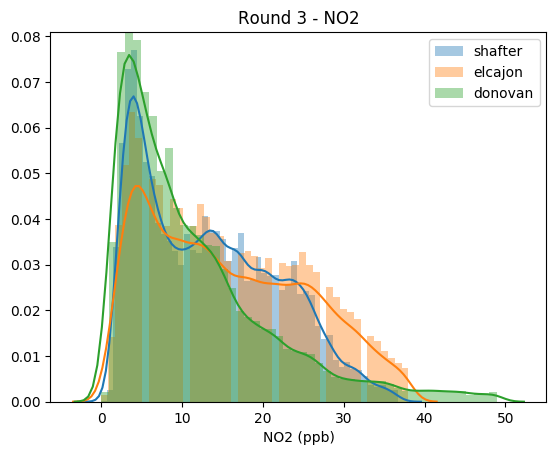
\includegraphics[width=\textwidth]{results/distributions/round3_no2.png}
\caption{Round 3}
\end{subfigure}
\caption{NO2 over rounds}
\label{fig:no2-rounds}
\end{figure}

\begin{figure}[H]
\centering
\begin{subfigure}{0.32\textwidth}
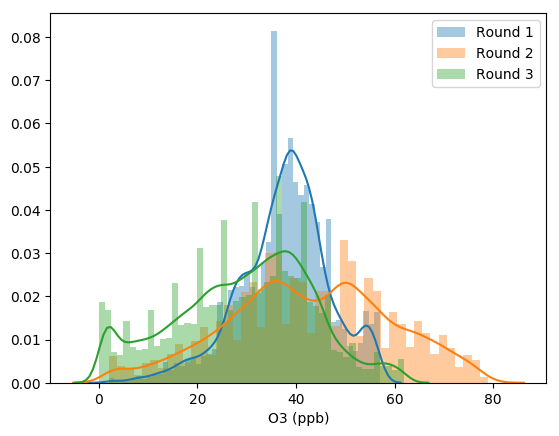
\includegraphics[width=\textwidth]{results/distributions/location_donovan_o3.png}
\caption{Round 1}
\end{subfigure}
\begin{subfigure}{0.32\textwidth}
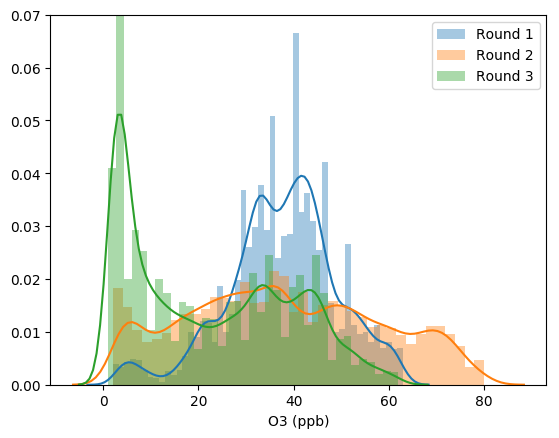
\includegraphics[width=\textwidth]{results/distributions/location_elcajon_o3.png}
\caption{Round 2}
\end{subfigure}
\begin{subfigure}{0.32\textwidth}
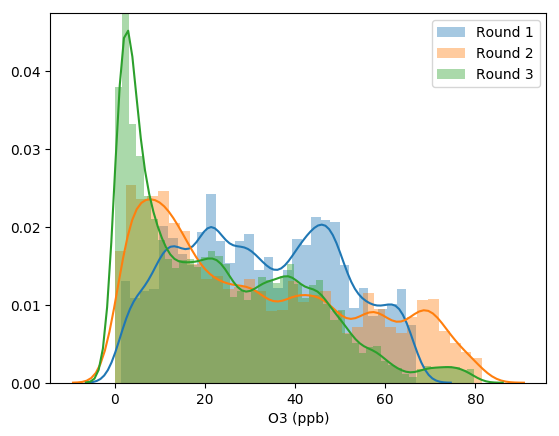
\includegraphics[width=\textwidth]{results/distributions/location_shafter_o3.png}
\caption{Round 3}
\end{subfigure}
\caption{O3 at locations}
\label{fig:o3-locations}
\end{figure}

\begin{figure}[H]
\centering
\begin{subfigure}{0.32\textwidth}
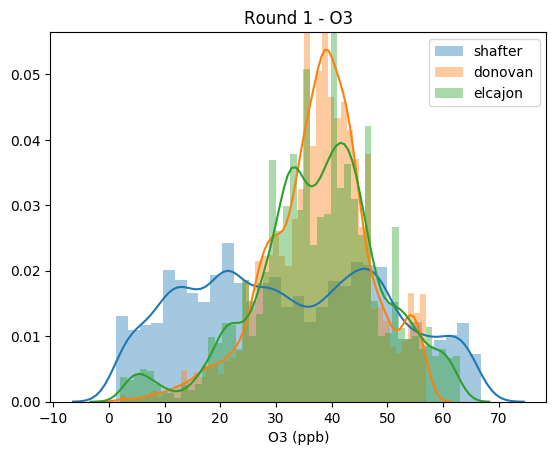
\includegraphics[width=\textwidth]{results/distributions/round1_o3.png}
\caption{Round 1}
\end{subfigure}
\begin{subfigure}{0.32\textwidth}
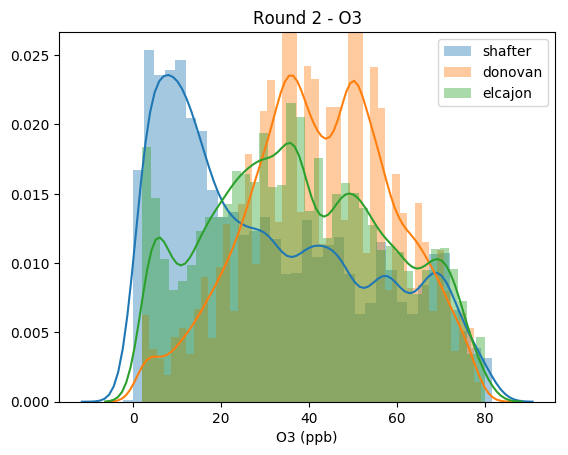
\includegraphics[width=\textwidth]{results/distributions/round2_o3.png}
\caption{Round 2}
\end{subfigure}
\begin{subfigure}{0.32\textwidth}
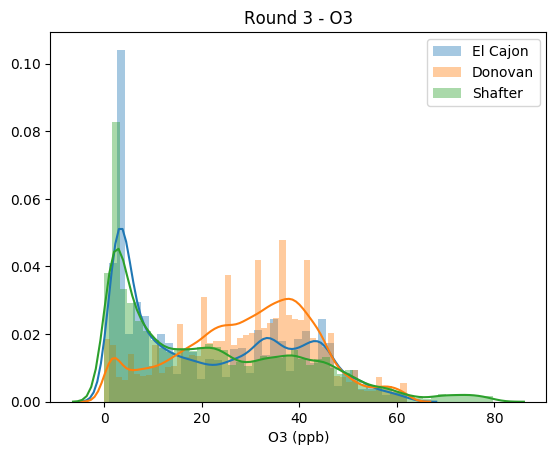
\includegraphics[width=\textwidth]{results/distributions/round3_o3.png}
\caption{Round 3}
\end{subfigure}
\caption{O3 over rounds}
\label{fig:o3-rounds}
\end{figure}


\section{Basic calibration results}

A calibration model takes in sensor readings and environment
variables and outputs pollutant levels. In this basic setup,
we train a model for each board.
We aim to train models that are robust after moving location.

\begin{table}[H]
\centering
\begin{tabular}{|l|l|}
\hline
\textbf{Level 0} & Train on location A and test on location A \\ \hline
\textbf{Level 1} & Train on location A and test on location B \\ \hline
\textbf{Level 2} & Train on location A and B and test on location C \\ \hline
\textbf{Level 3} & Train on location A, B, and C and test on location A \\ \hline
\end{tabular}
\caption{Description of different types of benchmarks.}
\label{tab:levels}
\end{table}

We benchmark four different models: linear regression (linear), random forest regressors based on \citep{Zimmerman2018},
a 2-layer neural network (NN[2]), and a 4-layer neural network (NN[4]). The ideal model will
both predict pollutant levels accurately and
generalize across locations.

To benchmark, we first take our datasets (25 total, see \autoref{tab:board-rotations}), and partition each into training and test sets (20\% reserved for testing).
We perform several types of benchmarks,
each to learn about the transferrability of each model (see \autoref{tab:levels}).
In general, we expect Level 0 and Level 3 performance to be the best, as they involve training and testing on data from the same distribution. Furthermore, we expected Level 2 to have lower error than Level 1, because Level 2 is trained on more data and a wider distribution of data (two locations vs one location).
If a model's Level 1 and Level 2 error are close to Level 0 and Level 3, then the model transfers well. Otherwise, the model overfits to its location.


These raw results are in \autoref{sec:simpleresults}. 
We split results into train vs. test
results, where we expect train performance
to be better than test.
Overall, we see that random forests have the lowest Level 0 and Level 3 error. This is consistent with results we see in \citet{Zimmerman2018}. 
We observe when comparing Level 1 error difference (Level 1 train minus Level 1 test), random forests suffer great
drops in performance.
This hints that RFs are overfitting to the training data, even if they
report the lowest test error for Level 0 and Level 3.  See \autoref{fig:generalization} for 
details.

\begin{figure}[H]
\centering
\begin{subfigure}{0.45\textwidth}
\includegraphics[width=\textwidth]{\baselinedir/NO2" "MAE_difference.png}
\caption{NO2}
\end{subfigure}
\begin{subfigure}{0.45\textwidth}
\includegraphics[width=\textwidth]{\baselinedir/O3" "MAE_difference.png}
\caption{O3}
\end{subfigure}
\caption{Difference plots. Train minus test errors for various models. A smaller value means that the models transfer better.}
\label{fig:generalization}
\end{figure}

\section{Neural representation learning}

We now present split-neural network results: we split
up calibration into two stages, a sensor model
and a pollutant model, which we will call $s_i$ and $c$
respectively.
Given a sensor readings $x$ from board $i$,
and environment readings $e$
we obtain a calibrated reading $y$ by simply passing it through
the sensor model, then the pollutant model, i.e.
\begin{align*}
    y = c(s_i(x), e)
\end{align*}
We can learn individual sensor models for each board,
but the pollutant model is shared across boards. This allows
us to pool data across boards to learn the pollutant model.
Furthermore, environment variables are only 
included in the pollutant model, which hopefully enables
a stronger fit with a very complex pollutant model.

Each $s_i(x)$ outputs a ``sensor representation'', which is chosen
to be some fixed dimension $d$. We hope that the sensor representation
contains the minimal information to produce calibrated readings.

We experiment with each $s_i$ being a linear regression model,
and $c$ being a deep neural network (two layers, 100 width ReLU). 
Each set of data we collect
is identified by a triplet of information (round, location, board number). In total, we have 25 of such datasets as defined in \autoref{tab:board-rotations}. To benchmark these split models, we train on all of these datasets, but
hold one triple out, resulting in a
total training set size of 24 datasets and test size of 1 dataset. This results in a total of 25 experiments
for which we boxplot the results.
We compare the split models to our four static models (Linear, NN[2], NN[4], Random Forest) by comparing the Split-NN performance on the held out dataset to the Level 2 performance of the four models.
Level 2 performance corresponds to training on two locations
and testing on the third. The split model has access to the same training data as the Level 2 models, but with the addition of data from other boards. The hope is this additional board data can help improve upon Level 2 performance, which can be thought of as the ``best'' possible transfer performance.

\begin{figure}[H]
\begin{subfigure}{0.49\textwidth}
\includegraphics[width=\textwidth]{\splitdir/linear/no2mae.png}
\caption{NO2 MAE}
\end{subfigure}
\begin{subfigure}{0.49\textwidth}
\includegraphics[width=\textwidth]{\splitdir/linear/o3mae.png}
\caption{O3 MAE}
\end{subfigure}
\begin{subfigure}{0.49\textwidth}
\includegraphics[width=\textwidth]{\splitdir/linear/no2cvmae.png}
\caption{NO2 CvMAE}
\end{subfigure}
\begin{subfigure}{0.49\textwidth}
\includegraphics[width=\textwidth]{\splitdir/linear/o3cvmae.png}
\caption{O3 CvMAE}
\end{subfigure}
\caption{Comparison of errors of Split NN and Linear. Training size corresponds to a Level 1 or Level 2 comparison.}
\end{figure}

\begin{figure}[H]
\begin{subfigure}{0.49\textwidth}
\includegraphics[width=\textwidth]{\splitdir/nn-2/no2mae.png}
\caption{NO2 MAE}
\end{subfigure}
\begin{subfigure}{0.49\textwidth}
\includegraphics[width=\textwidth]{\splitdir/nn-2/o3mae.png}
\caption{O3 MAE}
\end{subfigure}
\begin{subfigure}{0.49\textwidth}
\includegraphics[width=\textwidth]{\splitdir/nn-2/no2cvmae.png}
\caption{NO2 CvMAE}
\end{subfigure}
\begin{subfigure}{0.49\textwidth}
\includegraphics[width=\textwidth]{\splitdir/nn-2/o3cvmae.png}
\caption{O3 CvMAE}
\end{subfigure}
\caption{Comparison of errors of Split NN and NN[2]. Training size corresponds to a Level 1 or Level 2 comparison.}
\end{figure}

\begin{figure}[H]
\begin{subfigure}{0.49\textwidth}
\includegraphics[width=\textwidth]{\splitdir/nn-4/no2mae.png}
\caption{NO2 MAE}
\end{subfigure}
\begin{subfigure}{0.49\textwidth}
\includegraphics[width=\textwidth]{\splitdir/nn-4/o3mae.png}
\caption{O3 MAE}
\end{subfigure}
\begin{subfigure}{0.49\textwidth}
\includegraphics[width=\textwidth]{\splitdir/nn-4/no2cvmae.png}
\caption{NO2 CvMAE}
\end{subfigure}
\begin{subfigure}{0.49\textwidth}
\includegraphics[width=\textwidth]{\splitdir/nn-4/o3cvmae.png}
\caption{O3 CvMAE}
\end{subfigure}
\caption{Comparison of errors of Split NN and NN[4]. Training size corresponds to a Level 1 or Level 2 comparison.}
\end{figure}

\begin{figure}[H]
\begin{subfigure}{0.49\textwidth}
\includegraphics[width=\textwidth]{\splitdir/subu/no2mae.png}
\caption{NO2 MAE}
\end{subfigure}
\begin{subfigure}{0.49\textwidth}
\includegraphics[width=\textwidth]{\splitdir/subu/o3mae.png}
\caption{O3 MAE}
\end{subfigure}
\begin{subfigure}{0.49\textwidth}
\includegraphics[width=\textwidth]{\splitdir/subu/no2cvmae.png}
\caption{NO2 CvMAE}
\end{subfigure}
\begin{subfigure}{0.49\textwidth}
\includegraphics[width=\textwidth]{\splitdir/subu/o3cvmae.png}
\caption{O3 CvMAE}
\end{subfigure}
\caption{Comparison of errors of Split NN and Subu. Training size corresponds to a Level 1 or Level 2 comparison.}
\end{figure}

To further accentuate the improvement, we can compare
the difference in performance between Split-NN and the four models. In these plots, a more negative value corresponds to a larger improvement.

\begin{figure}[H]
\begin{subfigure}{0.49\textwidth}
\includegraphics[width=\textwidth]{\splitdir/linear/no2mae-diff.png}
\caption{NO2 MAE Improvement}
\end{subfigure}
\begin{subfigure}{0.49\textwidth}
\includegraphics[width=\textwidth]{\splitdir/linear/o3mae-diff.png}
\caption{O3 MAE Improvement}
\end{subfigure}
\begin{subfigure}{0.49\textwidth}
\includegraphics[width=\textwidth]{\splitdir/linear/no2cvmae-diff.png}
\caption{NO2 CvMAE Improvement}
\end{subfigure}
\begin{subfigure}{0.49\textwidth}
\includegraphics[width=\textwidth]{\splitdir/linear/o3cvmae-diff.png}
\caption{O3 CvMAE Improvement}
\end{subfigure}
\caption{Comparison of errors of Split NN and Linear.}
\end{figure}

\begin{figure}[H]
\begin{subfigure}{0.49\textwidth}
\includegraphics[width=\textwidth]{\splitdir/nn-2/no2mae-diff.png}
\caption{NO2 MAE Improvement}
\end{subfigure}
\begin{subfigure}{0.49\textwidth}
\includegraphics[width=\textwidth]{\splitdir/nn-2/o3mae-diff.png}
\caption{O3 MAE Improvement}
\end{subfigure}
\begin{subfigure}{0.49\textwidth}
\includegraphics[width=\textwidth]{\splitdir/nn-2/no2cvmae-diff.png}
\caption{NO2 CvMAE Improvement}
\end{subfigure}
\begin{subfigure}{0.49\textwidth}
\includegraphics[width=\textwidth]{\splitdir/nn-2/o3cvmae-diff.png}
\caption{O3 CvMAE Improvement}
\end{subfigure}
\caption{Comparison of errors of Split NN and NN[2].}
\end{figure}

\begin{figure}[H]
\begin{subfigure}{0.49\textwidth}
\includegraphics[width=\textwidth]{\splitdir/nn-4/no2mae-diff.png}
\caption{NO2 MAE Improvement}
\end{subfigure}
\begin{subfigure}{0.49\textwidth}
\includegraphics[width=\textwidth]{\splitdir/nn-4/o3mae-diff.png}
\caption{O3 MAE Improvement}
\end{subfigure}
\begin{subfigure}{0.49\textwidth}
\includegraphics[width=\textwidth]{\splitdir/nn-4/no2cvmae-diff.png}
\caption{NO2 CvMAE Improvement}
\end{subfigure}
\begin{subfigure}{0.49\textwidth}
\includegraphics[width=\textwidth]{\splitdir/nn-4/o3cvmae-diff.png}
\caption{O3 CvMAE Improvement}
\end{subfigure}
\caption{Comparison of errors of Split NN and NN[4].}
\end{figure}

\begin{figure}[H]
\begin{subfigure}{0.49\textwidth}
\includegraphics[width=\textwidth]{\splitdir/subu/no2mae-diff.png}
\caption{NO2 MAE Improvement}
\end{subfigure}
\begin{subfigure}{0.49\textwidth}
\includegraphics[width=\textwidth]{\splitdir/subu/o3mae-diff.png}
\caption{O3 MAE Improvement}
\end{subfigure}
\begin{subfigure}{0.49\textwidth}
\includegraphics[width=\textwidth]{\splitdir/subu/no2cvmae-diff.png}
\caption{NO2 CvMAE Improvement}
\end{subfigure}
\begin{subfigure}{0.49\textwidth}
\includegraphics[width=\textwidth]{\splitdir/subu/o3cvmae-diff.png}
\caption{O3 CvMAE Improvement}
\end{subfigure}
\caption{Comparison of errors of Split NN and Subu.}
\end{figure}

\renewcommand{\thetable}{\Alph{section}.\arabic{table}}

\section{Summaries of data for each location and round}
\label{sec:summaryresults}

\begin{table}[H]
\scriptsize
\begin{tabular}{llrrrrr}
\toprule
        &       &        epa-no2 &         epa-o3 &    temperature &       pressure &       humidity \\
Location & {} &                &                &                &                &                \\
\midrule
donovan & count &  100788.000000 &  100788.000000 &  100788.000000 &  100788.000000 &  100788.000000 \\
        & mean &      10.434149 &      33.742201 &      24.169544 &     991.767126 &      45.937553 \\
        & std &      10.806435 &      15.377371 &       5.623704 &       3.225557 &      21.965513 \\
        & min &       0.000000 &       0.000000 &      13.900000 &     982.820000 &       4.086000 \\
        & 25\% &       3.000000 &      24.000000 &      20.100000 &     989.530000 &      27.245000 \\
        & 50\% &       7.000000 &      35.000000 &      22.620000 &     991.460000 &      49.513000 \\
        & 75\% &      14.000000 &      43.000000 &      27.000000 &     993.610000 &      64.396000 \\
        & max &     157.000000 &      96.000000 &      49.710000 &    1004.160000 &      92.753000 \\
elcajon & count &   97412.000000 &   97412.000000 &   97412.000000 &   97412.000000 &   97412.000000 \\
        & mean &      12.914015 &      29.331499 &      24.341702 &     997.287606 &      43.923309 \\
        & std &       9.732012 &      19.337040 &       8.232391 &       3.507203 &      20.076611 \\
        & min &       0.000000 &       1.000000 &       5.430000 &     989.230000 &       2.733000 \\
        & 25\% &       5.000000 &      11.000000 &      18.570000 &     994.880000 &      28.623000 \\
        & 50\% &      10.000000 &      31.000000 &      23.380000 &     996.890000 &      45.052500 \\
        & 75\% &      20.000000 &      43.000000 &      29.700000 &     999.450000 &      61.166250 \\
        & max &      66.000000 &      95.000000 &      49.790000 &    1010.480000 &      85.827000 \\
shafter & count &  119785.000000 &  119785.000000 &  119785.000000 &  119785.000000 &  119785.000000 \\
        & mean &      12.578259 &      26.357091 &      22.100842 &    1003.882723 &      45.804388 \\
        & std &       9.078981 &      20.739128 &       8.184091 &       5.595797 &      18.072375 \\
        & min &       0.000000 &       0.000000 &       4.010000 &     872.755556 &       6.349000 \\
        & 25\% &       4.700000 &       7.800000 &      16.155556 &     999.750000 &      30.585000 \\
        & 50\% &      10.800000 &      22.300000 &      21.040000 &    1003.990000 &      46.763000 \\
        & 75\% &      19.000000 &      41.200000 &      27.200000 &    1007.400000 &      60.965000 \\
        & max &     594.600000 &     110.400000 &      47.700000 &    1019.580000 &      85.047000 \\
\bottomrule
\end{tabular}

\caption{Summary of dataset grouped by location}
\label{tab:locationsummary}
\end{table}

\begin{table}[H]
\scriptsize
\begin{tabular}{llrrrrr}
\toprule
  &       &        epa-no2 &         epa-o3 &    temperature &       pressure &       humidity \\
Round & {} &                &                &                &                &                \\
\midrule
1 & count &   49779.000000 &   49779.000000 &   49779.000000 &   49779.000000 &   49779.000000 \\
  & mean &       5.510173 &      36.010330 &      26.061407 &     994.458473 &      48.324276 \\
  & std &       5.472665 &      13.867920 &       6.776587 &       4.786306 &      19.538803 \\
  & min &       0.000000 &       1.300000 &      13.100000 &     872.755556 &       9.644000 \\
  & 25\% &       2.000000 &      28.000000 &      20.900000 &     990.920000 &      31.793000 \\
  & 50\% &       3.700000 &      37.300000 &      24.600000 &     995.240000 &      50.513000 \\
  & 75\% &       6.600000 &      45.000000 &      30.130000 &     997.640000 &      61.526500 \\
  & max &      57.000000 &     110.400000 &      47.700000 &    1002.940000 &      92.753000 \\
2 & count &   75129.000000 &   75129.000000 &   75129.000000 &   75129.000000 &   75129.000000 \\
  & mean &      11.915875 &      36.973669 &      25.952835 &     995.989062 &      41.511134 \\
  & std &       9.583090 &      21.259456 &       7.576508 &       6.074511 &      19.756994 \\
  & min &      -1.000000 &      -2.400000 &      12.000000 &     982.820000 &       4.420000 \\
  & 25\% &       5.000000 &      19.200000 &      20.000000 &     990.990000 &      23.461000 \\
  & 50\% &       8.000000 &      36.000000 &      24.400000 &     995.420000 &      41.539000 \\
  & 75\% &      17.900000 &      53.000000 &      31.710000 &    1000.710000 &      56.961000 \\
  & max &      82.000000 &      96.000000 &      48.180000 &    1009.890000 &      87.562000 \\
3 & count &  193077.000000 &  193077.000000 &  193077.000000 &  193077.000000 &  193077.000000 \\
  & mean &      13.708376 &      25.092386 &      21.791316 &     999.732162 &      45.945741 \\
  & std &      10.225285 &      17.803517 &       7.275538 &       6.707979 &      20.012530 \\
  & min &      -3.000000 &      -6.200000 &       4.010000 &     986.770000 &       2.733000 \\
  & 25\% &       5.100000 &       8.000000 &      17.190000 &     994.300000 &      30.192000 \\
  & 50\% &      11.600000 &      24.700000 &      21.000000 &     999.090000 &      48.470000 \\
  & 75\% &      20.000000 &      38.500000 &      25.780000 &    1004.690000 &      63.450000 \\
  & max &     594.600000 &      87.900000 &      49.790000 &    1019.580000 &      85.440000 \\
\bottomrule
\end{tabular}

\caption{Summary of dataset grouped by round}
\label{tab:roundsummary}
\end{table}

\section{Raw results for simple calibration models}
\label{sec:simpleresults}

\subsection{Benchmarks for linear regression}
\label{sec:results-lr}

\begin{table}[H]
\centering
\scriptsize
\begin{tabular}{llrrrr}
\toprule
{} &             Model &   NO2 MAE &    O3 MAE &  NO2 CvMAE &  O3 CvMAE \\
\midrule
8  &  (2, donovan, 15) &  5.027835 &  6.232665 &   0.473339 &  0.145164 \\
6  &  (2, donovan, 18) &  4.746318 &  5.570541 &   0.456590 &  0.130750 \\
7  &  (2, donovan, 20) &  4.842058 &  6.238720 &   0.466330 &  0.146309 \\
0  &  (2, elcajon, 17) &  2.698047 &  4.559094 &   0.239658 &  0.119533 \\
1  &  (2, elcajon, 19) &  2.655985 &  5.337602 &   0.235975 &  0.139820 \\
2  &  (2, elcajon, 21) &  2.433894 &  4.449262 &   0.216725 &  0.116582 \\
3  &  (2, shafter, 11) &  3.819798 &  5.578007 &   0.284526 &  0.176786 \\
4  &  (2, shafter, 12) &  3.642114 &  5.607741 &   0.270953 &  0.177336 \\
5  &  (2, shafter, 13) &  3.936738 &  6.036189 &   0.290300 &  0.192189 \\
15 &  (3, donovan, 11) &  3.031544 &  3.997557 &   0.255644 &  0.133657 \\
16 &  (3, donovan, 12) &  2.975868 &  4.427616 &   0.250879 &  0.148093 \\
17 &  (3, donovan, 13) &  3.358886 &  4.542841 &   0.286095 &  0.152702 \\
11 &  (3, elcajon, 15) &  2.297309 &  3.423670 &   0.144815 &  0.151805 \\
9  &  (3, elcajon, 18) &  2.561304 &  3.105009 &   0.160601 &  0.137941 \\
10 &  (3, elcajon, 20) &  2.286381 &  3.381494 &   0.143313 &  0.150300 \\
12 &  (3, shafter, 17) &  2.975214 &  3.633606 &   0.217359 &  0.159339 \\
13 &  (3, shafter, 19) &  3.067352 &  3.801227 &   0.220440 &  0.166161 \\
14 &  (3, shafter, 21) &  2.588553 &  3.702099 &   0.189111 &  0.162343 \\
24 &  (4, donovan, 17) &  4.441255 &  8.398913 &   0.583048 &  0.225941 \\
25 &  (4, donovan, 19) &  3.834746 &  7.323790 &   0.506982 &  0.196196 \\
26 &  (4, donovan, 21) &  4.466916 &  7.095089 &   0.586417 &  0.190867 \\
18 &  (4, elcajon, 11) &  2.381288 &  2.712045 &   0.123120 &  0.152712 \\
19 &  (4, elcajon, 12) &  3.098652 &  3.233550 &   0.160211 &  0.182077 \\
20 &  (4, elcajon, 13) &  2.734451 &  3.283903 &   0.141341 &  0.185145 \\
23 &  (4, shafter, 15) &  3.002186 &  3.810681 &   0.241866 &  0.193013 \\
21 &  (4, shafter, 18) &  2.510484 &  2.808885 &   0.203406 &  0.140197 \\
22 &  (4, shafter, 20) &  2.543909 &  2.862168 &   0.206222 &  0.142653 \\
\bottomrule
\end{tabular}

\caption{Level 0 train results for linear regression}
\end{table}
\begin{table}[H]
\centering
\scriptsize
\begin{tabular}{llrrrrrrrrrrrrrr}
\toprule
{} &             Model &  NO2 CvMAE &   NO2 MAE &   NO2 MBE &    NO2 MSE &   NO2 R\textasciicircum2 &  NO2 crMSE &  NO2 rMSE &  O3 CvMAE &    O3 MAE &    O3 MBE &      O3 MSE &    O3 R\textasciicircum2 &   O3 crMSE &    O3 rMSE \\
\midrule
8  &  (2, donovan, 15) &   0.502952 &  5.356068 &  1.207103 &  84.356872 &  0.369497 &   9.104931 &  9.184600 &  0.171683 &  7.380878 &  1.620165 &  101.408904 &  0.660706 &   9.939013 &  10.070199 \\
6  &  (2, donovan, 18) &   0.521589 &  5.472068 &  1.928734 &  95.328335 &  0.297971 &   9.571224 &  9.763623 &  0.155519 &  6.613003 &  0.186258 &   86.547567 &  0.693264 &   9.301230 &   9.303094 \\
7  &  (2, donovan, 20) &   0.524009 &  5.522302 &  0.743507 &  85.953905 &  0.361247 &   9.241272 &  9.271133 &  0.169797 &  7.196145 &  1.294524 &   99.007696 &  0.647560 &   9.865693 &   9.950261 \\
0  &  (2, elcajon, 17) &   0.283159 &  3.184891 & -0.829539 &  19.055407 &  0.715360 &   4.285705 &  4.365250 &  0.151976 &  5.881672 &  0.960097 &   56.608272 &  0.866436 &   7.462338 &   7.523847 \\
1  &  (2, elcajon, 19) &   0.267745 &  3.011492 & -0.786412 &  18.191240 &  0.729810 &   4.191992 &  4.265119 &  0.171726 &  6.621740 &  1.224656 &   74.445887 &  0.824927 &   8.540849 &   8.628203 \\
2  &  (2, elcajon, 21) &   0.254546 &  2.894617 &  0.234951 &  17.577710 &  0.740132 &   4.185989 &  4.192578 &  0.145349 &  5.610693 & -0.005434 &   53.279390 &  0.874668 &   7.299271 &   7.299273 \\
3  &  (2, shafter, 11) &   0.350422 &  4.750222 & -0.149093 &  46.705791 &  0.452650 &   6.832537 &  6.834163 &  0.261026 &  8.222371 & -1.338942 &  121.533561 &  0.776911 &  10.942614 &  11.024226 \\
4  &  (2, shafter, 12) &   0.331302 &  4.447061 &  0.228306 &  39.551147 &  0.536775 &   6.284825 &  6.288970 &  0.206513 &  6.506042 & -0.537655 &   74.684995 &  0.858096 &   8.625307 &   8.642048 \\
5  &  (2, shafter, 13) &   0.338705 &  4.571687 & -0.732873 &  40.994675 &  0.529286 &   6.360627 &  6.402708 &  0.232688 &  7.373790 &  0.444752 &   96.906288 &  0.820112 &   9.834047 &   9.844099 \\
15 &  (3, donovan, 11) &   0.290715 &  3.497531 &  0.168204 &  40.766892 &  0.679717 &   6.382680 &  6.384896 &  0.149371 &  4.448765 & -0.008428 &   38.624821 &  0.814402 &   6.214881 &   6.214887 \\
16 &  (3, donovan, 12) &   0.280582 &  3.372065 &  0.718885 &  38.994275 &  0.689527 &   6.203022 &  6.244540 &  0.166886 &  4.977496 &  0.225353 &   45.556271 &  0.781258 &   6.745775 &   6.749539 \\
17 &  (3, donovan, 13) &   0.321910 &  3.834315 &  0.229491 &  51.510997 &  0.616357 &   7.173446 &  7.177116 &  0.178732 &  5.317755 &  0.391164 &   51.637687 &  0.753602 &   7.175282 &   7.185937 \\
11 &  (3, elcajon, 15) &   0.169998 &  2.713472 & -0.535505 &  12.570339 &  0.878159 &   3.504793 &  3.545467 &  0.183740 &  4.128872 & -0.626230 &   31.219820 &  0.898477 &   5.552266 &   5.587470 \\
9  &  (3, elcajon, 18) &   0.195013 &  3.112672 & -0.097291 &  17.828047 &  0.827037 &   4.221206 &  4.222327 &  0.171306 &  3.861852 & -1.385070 &   28.428616 &  0.907926 &   5.148805 &   5.331849 \\
10 &  (3, elcajon, 20) &   0.157671 &  2.513090 &  0.346674 &  11.061324 &  0.892557 &   3.307740 &  3.325857 &  0.173672 &  3.922748 & -0.285295 &   29.998760 &  0.902827 &   5.469677 &   5.477112 \\
12 &  (3, shafter, 17) &   0.239940 &  3.284343 &  0.131269 &  22.645272 &  0.715309 &   4.756894 &  4.758705 &  0.186006 &  4.202592 & -0.408652 &   35.751006 &  0.906071 &   5.965233 &   5.979214 \\
13 &  (3, shafter, 19) &   0.240806 &  3.376456 &  0.272479 &  24.889888 &  0.693938 &   4.981530 &  4.988977 &  0.188865 &  4.291018 & -0.384494 &   40.929372 &  0.899494 &   6.386042 &   6.397607 \\
14 &  (3, shafter, 21) &   0.210358 &  2.879412 &  0.011439 &  17.565364 &  0.779172 &   4.191090 &  4.191105 &  0.186369 &  4.210788 &  0.120145 &   36.019752 &  0.905364 &   6.000443 &   6.001646 \\
24 &  (4, donovan, 17) &   0.615149 &  4.935584 & -1.119120 &  47.244500 &  0.302222 &   6.781745 &  6.873463 &  0.263737 &  9.565474 &  3.467672 &  153.288669 &  0.105674 &  11.885450 &  12.380980 \\
25 &  (4, donovan, 19) &   0.492158 &  4.066780 & -1.939447 &  26.927071 &  0.576912 &   4.813067 &  5.189130 &  0.221462 &  7.884556 &  6.956457 &   91.431999 &  0.479964 &   6.560466 &   9.562008 \\
26 &  (4, donovan, 21) &   0.488343 &  3.918168 & -1.453612 &  31.227058 &  0.538792 &   5.395746 &  5.588118 &  0.192470 &  6.980700 &  4.443966 &   98.232729 &  0.426885 &   8.859114 &   9.911243 \\
18 &  (4, elcajon, 11) &   0.141903 &  2.742548 &  0.286675 &  14.526424 &  0.857145 &   3.800558 &  3.811355 &  0.178339 &  3.188623 & -0.102435 &   19.744484 &  0.933701 &   4.442296 &   4.443477 \\
19 &  (4, elcajon, 12) &   0.188551 &  3.644105 & -1.182486 &  23.847732 &  0.765477 &   4.738086 &  4.883414 &  0.222241 &  3.973555 &  0.549150 &   32.909748 &  0.889493 &   5.710357 &   5.736702 \\
20 &  (4, elcajon, 13) &   0.166834 &  3.233265 & -0.119840 &  21.627452 &  0.791661 &   4.648988 &  4.650532 &  0.236179 &  4.180478 & -0.593235 &   37.725108 &  0.871515 &   6.113361 &   6.142077 \\
23 &  (4, shafter, 15) &   0.264236 &  3.298589 & -0.022578 &  20.505460 &  0.708680 &   4.528239 &  4.528295 &  0.211610 &  4.160323 & -0.145128 &   33.823756 &  0.879765 &   5.814008 &   5.815819 \\
21 &  (4, shafter, 18) &   0.228745 &  2.834217 & -0.001542 &  15.815600 &  0.777698 &   3.976883 &  3.976883 &  0.158389 &  3.176332 &  0.661127 &   19.152851 &  0.932207 &   4.326172 &   4.376397 \\
22 &  (4, shafter, 20) &   0.239203 &  2.969035 & -0.387849 &  17.749181 &  0.750865 &   4.195087 &  4.212978 &  0.178821 &  3.567077 & -0.228374 &   23.884073 &  0.914460 &   4.881795 &   4.887133 \\
\bottomrule
\end{tabular}

\caption{Level 0 test results for linear regression}
\end{table}

\begin{table}[H]
\centering
\scriptsize
\begin{tabular}{llrrrr}
\toprule
{} &             Model &   NO2 MAE &    O3 MAE &  NO2 CvMAE &  O3 CvMAE \\
\midrule
8  &  (2, donovan, 15) &  5.027835 &  6.232665 &   0.473339 &  0.145164 \\
6  &  (2, donovan, 18) &  4.746318 &  5.570541 &   0.456590 &  0.130750 \\
7  &  (2, donovan, 20) &  4.842058 &  6.238720 &   0.466330 &  0.146309 \\
0  &  (2, elcajon, 17) &  2.698047 &  4.559094 &   0.239658 &  0.119533 \\
1  &  (2, elcajon, 19) &  2.655985 &  5.337602 &   0.235975 &  0.139820 \\
2  &  (2, elcajon, 21) &  2.433894 &  4.449262 &   0.216725 &  0.116582 \\
3  &  (2, shafter, 11) &  3.819798 &  5.578007 &   0.284526 &  0.176786 \\
4  &  (2, shafter, 12) &  3.642114 &  5.607741 &   0.270953 &  0.177336 \\
5  &  (2, shafter, 13) &  3.936738 &  6.036189 &   0.290300 &  0.192189 \\
15 &  (3, donovan, 11) &  3.031544 &  3.997557 &   0.255644 &  0.133657 \\
16 &  (3, donovan, 12) &  2.975868 &  4.427616 &   0.250879 &  0.148093 \\
17 &  (3, donovan, 13) &  3.358886 &  4.542841 &   0.286095 &  0.152702 \\
11 &  (3, elcajon, 15) &  2.297309 &  3.423670 &   0.144815 &  0.151805 \\
9  &  (3, elcajon, 18) &  2.561304 &  3.105009 &   0.160601 &  0.137941 \\
10 &  (3, elcajon, 20) &  2.286381 &  3.381494 &   0.143313 &  0.150300 \\
12 &  (3, shafter, 17) &  2.975214 &  3.633606 &   0.217359 &  0.159339 \\
13 &  (3, shafter, 19) &  3.067352 &  3.801227 &   0.220440 &  0.166161 \\
14 &  (3, shafter, 21) &  2.588553 &  3.702099 &   0.189111 &  0.162343 \\
24 &  (4, donovan, 17) &  4.441255 &  8.398913 &   0.583048 &  0.225941 \\
25 &  (4, donovan, 19) &  3.834746 &  7.323790 &   0.506982 &  0.196196 \\
26 &  (4, donovan, 21) &  4.466916 &  7.095089 &   0.586417 &  0.190867 \\
18 &  (4, elcajon, 11) &  2.381288 &  2.712045 &   0.123120 &  0.152712 \\
19 &  (4, elcajon, 12) &  3.098652 &  3.233550 &   0.160211 &  0.182077 \\
20 &  (4, elcajon, 13) &  2.734451 &  3.283903 &   0.141341 &  0.185145 \\
23 &  (4, shafter, 15) &  3.002186 &  3.810681 &   0.241866 &  0.193013 \\
21 &  (4, shafter, 18) &  2.510484 &  2.808885 &   0.203406 &  0.140197 \\
22 &  (4, shafter, 20) &  2.543909 &  2.862168 &   0.206222 &  0.142653 \\
\bottomrule
\end{tabular}

\caption{Level 1 train results for linear regression}
\end{table}
\begin{table}[H]
\centering
\scriptsize
\begin{tabular}{llrrrrrrrrrrrrrr}
\toprule
{} &             Model &  NO2 CvMAE &   NO2 MAE &   NO2 MBE &    NO2 MSE &   NO2 R\textasciicircum2 &  NO2 crMSE &  NO2 rMSE &  O3 CvMAE &    O3 MAE &    O3 MBE &      O3 MSE &    O3 R\textasciicircum2 &   O3 crMSE &    O3 rMSE \\
\midrule
8  &  (2, donovan, 15) &   0.502952 &  5.356068 &  1.207103 &  84.356872 &  0.369497 &   9.104931 &  9.184600 &  0.171683 &  7.380878 &  1.620165 &  101.408904 &  0.660706 &   9.939013 &  10.070199 \\
6  &  (2, donovan, 18) &   0.521589 &  5.472068 &  1.928734 &  95.328335 &  0.297971 &   9.571224 &  9.763623 &  0.155519 &  6.613003 &  0.186258 &   86.547567 &  0.693264 &   9.301230 &   9.303094 \\
7  &  (2, donovan, 20) &   0.524009 &  5.522302 &  0.743507 &  85.953905 &  0.361247 &   9.241272 &  9.271133 &  0.169797 &  7.196145 &  1.294524 &   99.007696 &  0.647560 &   9.865693 &   9.950261 \\
0  &  (2, elcajon, 17) &   0.283159 &  3.184891 & -0.829539 &  19.055407 &  0.715360 &   4.285705 &  4.365250 &  0.151976 &  5.881672 &  0.960097 &   56.608272 &  0.866436 &   7.462338 &   7.523847 \\
1  &  (2, elcajon, 19) &   0.267745 &  3.011492 & -0.786412 &  18.191240 &  0.729810 &   4.191992 &  4.265119 &  0.171726 &  6.621740 &  1.224656 &   74.445887 &  0.824927 &   8.540849 &   8.628203 \\
2  &  (2, elcajon, 21) &   0.254546 &  2.894617 &  0.234951 &  17.577710 &  0.740132 &   4.185989 &  4.192578 &  0.145349 &  5.610693 & -0.005434 &   53.279390 &  0.874668 &   7.299271 &   7.299273 \\
3  &  (2, shafter, 11) &   0.350422 &  4.750222 & -0.149093 &  46.705791 &  0.452650 &   6.832537 &  6.834163 &  0.261026 &  8.222371 & -1.338942 &  121.533561 &  0.776911 &  10.942614 &  11.024226 \\
4  &  (2, shafter, 12) &   0.331302 &  4.447061 &  0.228306 &  39.551147 &  0.536775 &   6.284825 &  6.288970 &  0.206513 &  6.506042 & -0.537655 &   74.684995 &  0.858096 &   8.625307 &   8.642048 \\
5  &  (2, shafter, 13) &   0.338705 &  4.571687 & -0.732873 &  40.994675 &  0.529286 &   6.360627 &  6.402708 &  0.232688 &  7.373790 &  0.444752 &   96.906288 &  0.820112 &   9.834047 &   9.844099 \\
15 &  (3, donovan, 11) &   0.290715 &  3.497531 &  0.168204 &  40.766892 &  0.679717 &   6.382680 &  6.384896 &  0.149371 &  4.448765 & -0.008428 &   38.624821 &  0.814402 &   6.214881 &   6.214887 \\
16 &  (3, donovan, 12) &   0.280582 &  3.372065 &  0.718885 &  38.994275 &  0.689527 &   6.203022 &  6.244540 &  0.166886 &  4.977496 &  0.225353 &   45.556271 &  0.781258 &   6.745775 &   6.749539 \\
17 &  (3, donovan, 13) &   0.321910 &  3.834315 &  0.229491 &  51.510997 &  0.616357 &   7.173446 &  7.177116 &  0.178732 &  5.317755 &  0.391164 &   51.637687 &  0.753602 &   7.175282 &   7.185937 \\
11 &  (3, elcajon, 15) &   0.169998 &  2.713472 & -0.535505 &  12.570339 &  0.878159 &   3.504793 &  3.545467 &  0.183740 &  4.128872 & -0.626230 &   31.219820 &  0.898477 &   5.552266 &   5.587470 \\
9  &  (3, elcajon, 18) &   0.195013 &  3.112672 & -0.097291 &  17.828047 &  0.827037 &   4.221206 &  4.222327 &  0.171306 &  3.861852 & -1.385070 &   28.428616 &  0.907926 &   5.148805 &   5.331849 \\
10 &  (3, elcajon, 20) &   0.157671 &  2.513090 &  0.346674 &  11.061324 &  0.892557 &   3.307740 &  3.325857 &  0.173672 &  3.922748 & -0.285295 &   29.998760 &  0.902827 &   5.469677 &   5.477112 \\
12 &  (3, shafter, 17) &   0.239940 &  3.284343 &  0.131269 &  22.645272 &  0.715309 &   4.756894 &  4.758705 &  0.186006 &  4.202592 & -0.408652 &   35.751006 &  0.906071 &   5.965233 &   5.979214 \\
13 &  (3, shafter, 19) &   0.240806 &  3.376456 &  0.272479 &  24.889888 &  0.693938 &   4.981530 &  4.988977 &  0.188865 &  4.291018 & -0.384494 &   40.929372 &  0.899494 &   6.386042 &   6.397607 \\
14 &  (3, shafter, 21) &   0.210358 &  2.879412 &  0.011439 &  17.565364 &  0.779172 &   4.191090 &  4.191105 &  0.186369 &  4.210788 &  0.120145 &   36.019752 &  0.905364 &   6.000443 &   6.001646 \\
24 &  (4, donovan, 17) &   0.615149 &  4.935584 & -1.119120 &  47.244500 &  0.302222 &   6.781745 &  6.873463 &  0.263737 &  9.565474 &  3.467672 &  153.288669 &  0.105674 &  11.885450 &  12.380980 \\
25 &  (4, donovan, 19) &   0.492158 &  4.066780 & -1.939447 &  26.927071 &  0.576912 &   4.813067 &  5.189130 &  0.221462 &  7.884556 &  6.956457 &   91.431999 &  0.479964 &   6.560466 &   9.562008 \\
26 &  (4, donovan, 21) &   0.488343 &  3.918168 & -1.453612 &  31.227058 &  0.538792 &   5.395746 &  5.588118 &  0.192470 &  6.980700 &  4.443966 &   98.232729 &  0.426885 &   8.859114 &   9.911243 \\
18 &  (4, elcajon, 11) &   0.141903 &  2.742548 &  0.286675 &  14.526424 &  0.857145 &   3.800558 &  3.811355 &  0.178339 &  3.188623 & -0.102435 &   19.744484 &  0.933701 &   4.442296 &   4.443477 \\
19 &  (4, elcajon, 12) &   0.188551 &  3.644105 & -1.182486 &  23.847732 &  0.765477 &   4.738086 &  4.883414 &  0.222241 &  3.973555 &  0.549150 &   32.909748 &  0.889493 &   5.710357 &   5.736702 \\
20 &  (4, elcajon, 13) &   0.166834 &  3.233265 & -0.119840 &  21.627452 &  0.791661 &   4.648988 &  4.650532 &  0.236179 &  4.180478 & -0.593235 &   37.725108 &  0.871515 &   6.113361 &   6.142077 \\
23 &  (4, shafter, 15) &   0.264236 &  3.298589 & -0.022578 &  20.505460 &  0.708680 &   4.528239 &  4.528295 &  0.211610 &  4.160323 & -0.145128 &   33.823756 &  0.879765 &   5.814008 &   5.815819 \\
21 &  (4, shafter, 18) &   0.228745 &  2.834217 & -0.001542 &  15.815600 &  0.777698 &   3.976883 &  3.976883 &  0.158389 &  3.176332 &  0.661127 &   19.152851 &  0.932207 &   4.326172 &   4.376397 \\
22 &  (4, shafter, 20) &   0.239203 &  2.969035 & -0.387849 &  17.749181 &  0.750865 &   4.195087 &  4.212978 &  0.178821 &  3.567077 & -0.228374 &   23.884073 &  0.914460 &   4.881795 &   4.887133 \\
\bottomrule
\end{tabular}

\caption{Level 1 test results for linear regression}
\end{table}

\begin{table}[H]
\centering
\scriptsize
\begin{tabular}{llrrrr}
\toprule
{} &             Model &   NO2 MAE &    O3 MAE &  NO2 CvMAE &  O3 CvMAE \\
\midrule
8  &  (2, donovan, 15) &  5.027835 &  6.232665 &   0.473339 &  0.145164 \\
6  &  (2, donovan, 18) &  4.746318 &  5.570541 &   0.456590 &  0.130750 \\
7  &  (2, donovan, 20) &  4.842058 &  6.238720 &   0.466330 &  0.146309 \\
0  &  (2, elcajon, 17) &  2.698047 &  4.559094 &   0.239658 &  0.119533 \\
1  &  (2, elcajon, 19) &  2.655985 &  5.337602 &   0.235975 &  0.139820 \\
2  &  (2, elcajon, 21) &  2.433894 &  4.449262 &   0.216725 &  0.116582 \\
3  &  (2, shafter, 11) &  3.819798 &  5.578007 &   0.284526 &  0.176786 \\
4  &  (2, shafter, 12) &  3.642114 &  5.607741 &   0.270953 &  0.177336 \\
5  &  (2, shafter, 13) &  3.936738 &  6.036189 &   0.290300 &  0.192189 \\
15 &  (3, donovan, 11) &  3.031544 &  3.997557 &   0.255644 &  0.133657 \\
16 &  (3, donovan, 12) &  2.975868 &  4.427616 &   0.250879 &  0.148093 \\
17 &  (3, donovan, 13) &  3.358886 &  4.542841 &   0.286095 &  0.152702 \\
11 &  (3, elcajon, 15) &  2.297309 &  3.423670 &   0.144815 &  0.151805 \\
9  &  (3, elcajon, 18) &  2.561304 &  3.105009 &   0.160601 &  0.137941 \\
10 &  (3, elcajon, 20) &  2.286381 &  3.381494 &   0.143313 &  0.150300 \\
12 &  (3, shafter, 17) &  2.975214 &  3.633606 &   0.217359 &  0.159339 \\
13 &  (3, shafter, 19) &  3.067352 &  3.801227 &   0.220440 &  0.166161 \\
14 &  (3, shafter, 21) &  2.588553 &  3.702099 &   0.189111 &  0.162343 \\
24 &  (4, donovan, 17) &  4.441255 &  8.398913 &   0.583048 &  0.225941 \\
25 &  (4, donovan, 19) &  3.834746 &  7.323790 &   0.506982 &  0.196196 \\
26 &  (4, donovan, 21) &  4.466916 &  7.095089 &   0.586417 &  0.190867 \\
18 &  (4, elcajon, 11) &  2.381288 &  2.712045 &   0.123120 &  0.152712 \\
19 &  (4, elcajon, 12) &  3.098652 &  3.233550 &   0.160211 &  0.182077 \\
20 &  (4, elcajon, 13) &  2.734451 &  3.283903 &   0.141341 &  0.185145 \\
23 &  (4, shafter, 15) &  3.002186 &  3.810681 &   0.241866 &  0.193013 \\
21 &  (4, shafter, 18) &  2.510484 &  2.808885 &   0.203406 &  0.140197 \\
22 &  (4, shafter, 20) &  2.543909 &  2.862168 &   0.206222 &  0.142653 \\
\bottomrule
\end{tabular}

\caption{Level 2 train results for linear regression}
\end{table}
\begin{table}[H]
\centering
\scriptsize
\begin{tabular}{llrrrrrrrrrrrrrr}
\toprule
{} &             Model &  NO2 CvMAE &   NO2 MAE &   NO2 MBE &    NO2 MSE &   NO2 R\textasciicircum2 &  NO2 crMSE &  NO2 rMSE &  O3 CvMAE &    O3 MAE &    O3 MBE &      O3 MSE &    O3 R\textasciicircum2 &   O3 crMSE &    O3 rMSE \\
\midrule
8  &  (2, donovan, 15) &   0.502952 &  5.356068 &  1.207103 &  84.356872 &  0.369497 &   9.104931 &  9.184600 &  0.171683 &  7.380878 &  1.620165 &  101.408904 &  0.660706 &   9.939013 &  10.070199 \\
6  &  (2, donovan, 18) &   0.521589 &  5.472068 &  1.928734 &  95.328335 &  0.297971 &   9.571224 &  9.763623 &  0.155519 &  6.613003 &  0.186258 &   86.547567 &  0.693264 &   9.301230 &   9.303094 \\
7  &  (2, donovan, 20) &   0.524009 &  5.522302 &  0.743507 &  85.953905 &  0.361247 &   9.241272 &  9.271133 &  0.169797 &  7.196145 &  1.294524 &   99.007696 &  0.647560 &   9.865693 &   9.950261 \\
0  &  (2, elcajon, 17) &   0.283159 &  3.184891 & -0.829539 &  19.055407 &  0.715360 &   4.285705 &  4.365250 &  0.151976 &  5.881672 &  0.960097 &   56.608272 &  0.866436 &   7.462338 &   7.523847 \\
1  &  (2, elcajon, 19) &   0.267745 &  3.011492 & -0.786412 &  18.191240 &  0.729810 &   4.191992 &  4.265119 &  0.171726 &  6.621740 &  1.224656 &   74.445887 &  0.824927 &   8.540849 &   8.628203 \\
2  &  (2, elcajon, 21) &   0.254546 &  2.894617 &  0.234951 &  17.577710 &  0.740132 &   4.185989 &  4.192578 &  0.145349 &  5.610693 & -0.005434 &   53.279390 &  0.874668 &   7.299271 &   7.299273 \\
3  &  (2, shafter, 11) &   0.350422 &  4.750222 & -0.149093 &  46.705791 &  0.452650 &   6.832537 &  6.834163 &  0.261026 &  8.222371 & -1.338942 &  121.533561 &  0.776911 &  10.942614 &  11.024226 \\
4  &  (2, shafter, 12) &   0.331302 &  4.447061 &  0.228306 &  39.551147 &  0.536775 &   6.284825 &  6.288970 &  0.206513 &  6.506042 & -0.537655 &   74.684995 &  0.858096 &   8.625307 &   8.642048 \\
5  &  (2, shafter, 13) &   0.338705 &  4.571687 & -0.732873 &  40.994675 &  0.529286 &   6.360627 &  6.402708 &  0.232688 &  7.373790 &  0.444752 &   96.906288 &  0.820112 &   9.834047 &   9.844099 \\
15 &  (3, donovan, 11) &   0.290715 &  3.497531 &  0.168204 &  40.766892 &  0.679717 &   6.382680 &  6.384896 &  0.149371 &  4.448765 & -0.008428 &   38.624821 &  0.814402 &   6.214881 &   6.214887 \\
16 &  (3, donovan, 12) &   0.280582 &  3.372065 &  0.718885 &  38.994275 &  0.689527 &   6.203022 &  6.244540 &  0.166886 &  4.977496 &  0.225353 &   45.556271 &  0.781258 &   6.745775 &   6.749539 \\
17 &  (3, donovan, 13) &   0.321910 &  3.834315 &  0.229491 &  51.510997 &  0.616357 &   7.173446 &  7.177116 &  0.178732 &  5.317755 &  0.391164 &   51.637687 &  0.753602 &   7.175282 &   7.185937 \\
11 &  (3, elcajon, 15) &   0.169998 &  2.713472 & -0.535505 &  12.570339 &  0.878159 &   3.504793 &  3.545467 &  0.183740 &  4.128872 & -0.626230 &   31.219820 &  0.898477 &   5.552266 &   5.587470 \\
9  &  (3, elcajon, 18) &   0.195013 &  3.112672 & -0.097291 &  17.828047 &  0.827037 &   4.221206 &  4.222327 &  0.171306 &  3.861852 & -1.385070 &   28.428616 &  0.907926 &   5.148805 &   5.331849 \\
10 &  (3, elcajon, 20) &   0.157671 &  2.513090 &  0.346674 &  11.061324 &  0.892557 &   3.307740 &  3.325857 &  0.173672 &  3.922748 & -0.285295 &   29.998760 &  0.902827 &   5.469677 &   5.477112 \\
12 &  (3, shafter, 17) &   0.239940 &  3.284343 &  0.131269 &  22.645272 &  0.715309 &   4.756894 &  4.758705 &  0.186006 &  4.202592 & -0.408652 &   35.751006 &  0.906071 &   5.965233 &   5.979214 \\
13 &  (3, shafter, 19) &   0.240806 &  3.376456 &  0.272479 &  24.889888 &  0.693938 &   4.981530 &  4.988977 &  0.188865 &  4.291018 & -0.384494 &   40.929372 &  0.899494 &   6.386042 &   6.397607 \\
14 &  (3, shafter, 21) &   0.210358 &  2.879412 &  0.011439 &  17.565364 &  0.779172 &   4.191090 &  4.191105 &  0.186369 &  4.210788 &  0.120145 &   36.019752 &  0.905364 &   6.000443 &   6.001646 \\
24 &  (4, donovan, 17) &   0.615149 &  4.935584 & -1.119120 &  47.244500 &  0.302222 &   6.781745 &  6.873463 &  0.263737 &  9.565474 &  3.467672 &  153.288669 &  0.105674 &  11.885450 &  12.380980 \\
25 &  (4, donovan, 19) &   0.492158 &  4.066780 & -1.939447 &  26.927071 &  0.576912 &   4.813067 &  5.189130 &  0.221462 &  7.884556 &  6.956457 &   91.431999 &  0.479964 &   6.560466 &   9.562008 \\
26 &  (4, donovan, 21) &   0.488343 &  3.918168 & -1.453612 &  31.227058 &  0.538792 &   5.395746 &  5.588118 &  0.192470 &  6.980700 &  4.443966 &   98.232729 &  0.426885 &   8.859114 &   9.911243 \\
18 &  (4, elcajon, 11) &   0.141903 &  2.742548 &  0.286675 &  14.526424 &  0.857145 &   3.800558 &  3.811355 &  0.178339 &  3.188623 & -0.102435 &   19.744484 &  0.933701 &   4.442296 &   4.443477 \\
19 &  (4, elcajon, 12) &   0.188551 &  3.644105 & -1.182486 &  23.847732 &  0.765477 &   4.738086 &  4.883414 &  0.222241 &  3.973555 &  0.549150 &   32.909748 &  0.889493 &   5.710357 &   5.736702 \\
20 &  (4, elcajon, 13) &   0.166834 &  3.233265 & -0.119840 &  21.627452 &  0.791661 &   4.648988 &  4.650532 &  0.236179 &  4.180478 & -0.593235 &   37.725108 &  0.871515 &   6.113361 &   6.142077 \\
23 &  (4, shafter, 15) &   0.264236 &  3.298589 & -0.022578 &  20.505460 &  0.708680 &   4.528239 &  4.528295 &  0.211610 &  4.160323 & -0.145128 &   33.823756 &  0.879765 &   5.814008 &   5.815819 \\
21 &  (4, shafter, 18) &   0.228745 &  2.834217 & -0.001542 &  15.815600 &  0.777698 &   3.976883 &  3.976883 &  0.158389 &  3.176332 &  0.661127 &   19.152851 &  0.932207 &   4.326172 &   4.376397 \\
22 &  (4, shafter, 20) &   0.239203 &  2.969035 & -0.387849 &  17.749181 &  0.750865 &   4.195087 &  4.212978 &  0.178821 &  3.567077 & -0.228374 &   23.884073 &  0.914460 &   4.881795 &   4.887133 \\
\bottomrule
\end{tabular}

\caption{Level 2 test results for linear regression}
\end{table}

\begin{table}[H]
\centering
\scriptsize
\begin{tabular}{llrrrr}
\toprule
{} &             Model &   NO2 MAE &    O3 MAE &  NO2 CvMAE &  O3 CvMAE \\
\midrule
8  &  (2, donovan, 15) &  5.027835 &  6.232665 &   0.473339 &  0.145164 \\
6  &  (2, donovan, 18) &  4.746318 &  5.570541 &   0.456590 &  0.130750 \\
7  &  (2, donovan, 20) &  4.842058 &  6.238720 &   0.466330 &  0.146309 \\
0  &  (2, elcajon, 17) &  2.698047 &  4.559094 &   0.239658 &  0.119533 \\
1  &  (2, elcajon, 19) &  2.655985 &  5.337602 &   0.235975 &  0.139820 \\
2  &  (2, elcajon, 21) &  2.433894 &  4.449262 &   0.216725 &  0.116582 \\
3  &  (2, shafter, 11) &  3.819798 &  5.578007 &   0.284526 &  0.176786 \\
4  &  (2, shafter, 12) &  3.642114 &  5.607741 &   0.270953 &  0.177336 \\
5  &  (2, shafter, 13) &  3.936738 &  6.036189 &   0.290300 &  0.192189 \\
15 &  (3, donovan, 11) &  3.031544 &  3.997557 &   0.255644 &  0.133657 \\
16 &  (3, donovan, 12) &  2.975868 &  4.427616 &   0.250879 &  0.148093 \\
17 &  (3, donovan, 13) &  3.358886 &  4.542841 &   0.286095 &  0.152702 \\
11 &  (3, elcajon, 15) &  2.297309 &  3.423670 &   0.144815 &  0.151805 \\
9  &  (3, elcajon, 18) &  2.561304 &  3.105009 &   0.160601 &  0.137941 \\
10 &  (3, elcajon, 20) &  2.286381 &  3.381494 &   0.143313 &  0.150300 \\
12 &  (3, shafter, 17) &  2.975214 &  3.633606 &   0.217359 &  0.159339 \\
13 &  (3, shafter, 19) &  3.067352 &  3.801227 &   0.220440 &  0.166161 \\
14 &  (3, shafter, 21) &  2.588553 &  3.702099 &   0.189111 &  0.162343 \\
24 &  (4, donovan, 17) &  4.441255 &  8.398913 &   0.583048 &  0.225941 \\
25 &  (4, donovan, 19) &  3.834746 &  7.323790 &   0.506982 &  0.196196 \\
26 &  (4, donovan, 21) &  4.466916 &  7.095089 &   0.586417 &  0.190867 \\
18 &  (4, elcajon, 11) &  2.381288 &  2.712045 &   0.123120 &  0.152712 \\
19 &  (4, elcajon, 12) &  3.098652 &  3.233550 &   0.160211 &  0.182077 \\
20 &  (4, elcajon, 13) &  2.734451 &  3.283903 &   0.141341 &  0.185145 \\
23 &  (4, shafter, 15) &  3.002186 &  3.810681 &   0.241866 &  0.193013 \\
21 &  (4, shafter, 18) &  2.510484 &  2.808885 &   0.203406 &  0.140197 \\
22 &  (4, shafter, 20) &  2.543909 &  2.862168 &   0.206222 &  0.142653 \\
\bottomrule
\end{tabular}

\caption{Level 3 train results for linear regression}
\end{table}
\begin{table}[H]
\centering
\scriptsize
\begin{tabular}{llrrrrrrrrrrrrrr}
\toprule
{} &             Model &  NO2 CvMAE &   NO2 MAE &   NO2 MBE &    NO2 MSE &   NO2 R\textasciicircum2 &  NO2 crMSE &  NO2 rMSE &  O3 CvMAE &    O3 MAE &    O3 MBE &      O3 MSE &    O3 R\textasciicircum2 &   O3 crMSE &    O3 rMSE \\
\midrule
8  &  (2, donovan, 15) &   0.502952 &  5.356068 &  1.207103 &  84.356872 &  0.369497 &   9.104931 &  9.184600 &  0.171683 &  7.380878 &  1.620165 &  101.408904 &  0.660706 &   9.939013 &  10.070199 \\
6  &  (2, donovan, 18) &   0.521589 &  5.472068 &  1.928734 &  95.328335 &  0.297971 &   9.571224 &  9.763623 &  0.155519 &  6.613003 &  0.186258 &   86.547567 &  0.693264 &   9.301230 &   9.303094 \\
7  &  (2, donovan, 20) &   0.524009 &  5.522302 &  0.743507 &  85.953905 &  0.361247 &   9.241272 &  9.271133 &  0.169797 &  7.196145 &  1.294524 &   99.007696 &  0.647560 &   9.865693 &   9.950261 \\
0  &  (2, elcajon, 17) &   0.283159 &  3.184891 & -0.829539 &  19.055407 &  0.715360 &   4.285705 &  4.365250 &  0.151976 &  5.881672 &  0.960097 &   56.608272 &  0.866436 &   7.462338 &   7.523847 \\
1  &  (2, elcajon, 19) &   0.267745 &  3.011492 & -0.786412 &  18.191240 &  0.729810 &   4.191992 &  4.265119 &  0.171726 &  6.621740 &  1.224656 &   74.445887 &  0.824927 &   8.540849 &   8.628203 \\
2  &  (2, elcajon, 21) &   0.254546 &  2.894617 &  0.234951 &  17.577710 &  0.740132 &   4.185989 &  4.192578 &  0.145349 &  5.610693 & -0.005434 &   53.279390 &  0.874668 &   7.299271 &   7.299273 \\
3  &  (2, shafter, 11) &   0.350422 &  4.750222 & -0.149093 &  46.705791 &  0.452650 &   6.832537 &  6.834163 &  0.261026 &  8.222371 & -1.338942 &  121.533561 &  0.776911 &  10.942614 &  11.024226 \\
4  &  (2, shafter, 12) &   0.331302 &  4.447061 &  0.228306 &  39.551147 &  0.536775 &   6.284825 &  6.288970 &  0.206513 &  6.506042 & -0.537655 &   74.684995 &  0.858096 &   8.625307 &   8.642048 \\
5  &  (2, shafter, 13) &   0.338705 &  4.571687 & -0.732873 &  40.994675 &  0.529286 &   6.360627 &  6.402708 &  0.232688 &  7.373790 &  0.444752 &   96.906288 &  0.820112 &   9.834047 &   9.844099 \\
15 &  (3, donovan, 11) &   0.290715 &  3.497531 &  0.168204 &  40.766892 &  0.679717 &   6.382680 &  6.384896 &  0.149371 &  4.448765 & -0.008428 &   38.624821 &  0.814402 &   6.214881 &   6.214887 \\
16 &  (3, donovan, 12) &   0.280582 &  3.372065 &  0.718885 &  38.994275 &  0.689527 &   6.203022 &  6.244540 &  0.166886 &  4.977496 &  0.225353 &   45.556271 &  0.781258 &   6.745775 &   6.749539 \\
17 &  (3, donovan, 13) &   0.321910 &  3.834315 &  0.229491 &  51.510997 &  0.616357 &   7.173446 &  7.177116 &  0.178732 &  5.317755 &  0.391164 &   51.637687 &  0.753602 &   7.175282 &   7.185937 \\
11 &  (3, elcajon, 15) &   0.169998 &  2.713472 & -0.535505 &  12.570339 &  0.878159 &   3.504793 &  3.545467 &  0.183740 &  4.128872 & -0.626230 &   31.219820 &  0.898477 &   5.552266 &   5.587470 \\
9  &  (3, elcajon, 18) &   0.195013 &  3.112672 & -0.097291 &  17.828047 &  0.827037 &   4.221206 &  4.222327 &  0.171306 &  3.861852 & -1.385070 &   28.428616 &  0.907926 &   5.148805 &   5.331849 \\
10 &  (3, elcajon, 20) &   0.157671 &  2.513090 &  0.346674 &  11.061324 &  0.892557 &   3.307740 &  3.325857 &  0.173672 &  3.922748 & -0.285295 &   29.998760 &  0.902827 &   5.469677 &   5.477112 \\
12 &  (3, shafter, 17) &   0.239940 &  3.284343 &  0.131269 &  22.645272 &  0.715309 &   4.756894 &  4.758705 &  0.186006 &  4.202592 & -0.408652 &   35.751006 &  0.906071 &   5.965233 &   5.979214 \\
13 &  (3, shafter, 19) &   0.240806 &  3.376456 &  0.272479 &  24.889888 &  0.693938 &   4.981530 &  4.988977 &  0.188865 &  4.291018 & -0.384494 &   40.929372 &  0.899494 &   6.386042 &   6.397607 \\
14 &  (3, shafter, 21) &   0.210358 &  2.879412 &  0.011439 &  17.565364 &  0.779172 &   4.191090 &  4.191105 &  0.186369 &  4.210788 &  0.120145 &   36.019752 &  0.905364 &   6.000443 &   6.001646 \\
24 &  (4, donovan, 17) &   0.615149 &  4.935584 & -1.119120 &  47.244500 &  0.302222 &   6.781745 &  6.873463 &  0.263737 &  9.565474 &  3.467672 &  153.288669 &  0.105674 &  11.885450 &  12.380980 \\
25 &  (4, donovan, 19) &   0.492158 &  4.066780 & -1.939447 &  26.927071 &  0.576912 &   4.813067 &  5.189130 &  0.221462 &  7.884556 &  6.956457 &   91.431999 &  0.479964 &   6.560466 &   9.562008 \\
26 &  (4, donovan, 21) &   0.488343 &  3.918168 & -1.453612 &  31.227058 &  0.538792 &   5.395746 &  5.588118 &  0.192470 &  6.980700 &  4.443966 &   98.232729 &  0.426885 &   8.859114 &   9.911243 \\
18 &  (4, elcajon, 11) &   0.141903 &  2.742548 &  0.286675 &  14.526424 &  0.857145 &   3.800558 &  3.811355 &  0.178339 &  3.188623 & -0.102435 &   19.744484 &  0.933701 &   4.442296 &   4.443477 \\
19 &  (4, elcajon, 12) &   0.188551 &  3.644105 & -1.182486 &  23.847732 &  0.765477 &   4.738086 &  4.883414 &  0.222241 &  3.973555 &  0.549150 &   32.909748 &  0.889493 &   5.710357 &   5.736702 \\
20 &  (4, elcajon, 13) &   0.166834 &  3.233265 & -0.119840 &  21.627452 &  0.791661 &   4.648988 &  4.650532 &  0.236179 &  4.180478 & -0.593235 &   37.725108 &  0.871515 &   6.113361 &   6.142077 \\
23 &  (4, shafter, 15) &   0.264236 &  3.298589 & -0.022578 &  20.505460 &  0.708680 &   4.528239 &  4.528295 &  0.211610 &  4.160323 & -0.145128 &   33.823756 &  0.879765 &   5.814008 &   5.815819 \\
21 &  (4, shafter, 18) &   0.228745 &  2.834217 & -0.001542 &  15.815600 &  0.777698 &   3.976883 &  3.976883 &  0.158389 &  3.176332 &  0.661127 &   19.152851 &  0.932207 &   4.326172 &   4.376397 \\
22 &  (4, shafter, 20) &   0.239203 &  2.969035 & -0.387849 &  17.749181 &  0.750865 &   4.195087 &  4.212978 &  0.178821 &  3.567077 & -0.228374 &   23.884073 &  0.914460 &   4.881795 &   4.887133 \\
\bottomrule
\end{tabular}

\caption{Level 3 test results for linear regression}
\end{table}

\subsection{Benchmarks for NN[2]}
\label{sec:results-nn2}

\begin{table}[H]
\centering
\scriptsize
\begin{tabular}{llrrrr}
\toprule
{} &             Model &   NO2 MAE &    O3 MAE &  NO2 CvMAE &  O3 CvMAE \\
\midrule
8  &  (2, donovan, 15) &  5.027835 &  6.232665 &   0.473339 &  0.145164 \\
6  &  (2, donovan, 18) &  4.746318 &  5.570541 &   0.456590 &  0.130750 \\
7  &  (2, donovan, 20) &  4.842058 &  6.238720 &   0.466330 &  0.146309 \\
0  &  (2, elcajon, 17) &  2.698047 &  4.559094 &   0.239658 &  0.119533 \\
1  &  (2, elcajon, 19) &  2.655985 &  5.337602 &   0.235975 &  0.139820 \\
2  &  (2, elcajon, 21) &  2.433894 &  4.449262 &   0.216725 &  0.116582 \\
3  &  (2, shafter, 11) &  3.819798 &  5.578007 &   0.284526 &  0.176786 \\
4  &  (2, shafter, 12) &  3.642114 &  5.607741 &   0.270953 &  0.177336 \\
5  &  (2, shafter, 13) &  3.936738 &  6.036189 &   0.290300 &  0.192189 \\
15 &  (3, donovan, 11) &  3.031544 &  3.997557 &   0.255644 &  0.133657 \\
16 &  (3, donovan, 12) &  2.975868 &  4.427616 &   0.250879 &  0.148093 \\
17 &  (3, donovan, 13) &  3.358886 &  4.542841 &   0.286095 &  0.152702 \\
11 &  (3, elcajon, 15) &  2.297309 &  3.423670 &   0.144815 &  0.151805 \\
9  &  (3, elcajon, 18) &  2.561304 &  3.105009 &   0.160601 &  0.137941 \\
10 &  (3, elcajon, 20) &  2.286381 &  3.381494 &   0.143313 &  0.150300 \\
12 &  (3, shafter, 17) &  2.975214 &  3.633606 &   0.217359 &  0.159339 \\
13 &  (3, shafter, 19) &  3.067352 &  3.801227 &   0.220440 &  0.166161 \\
14 &  (3, shafter, 21) &  2.588553 &  3.702099 &   0.189111 &  0.162343 \\
24 &  (4, donovan, 17) &  4.441255 &  8.398913 &   0.583048 &  0.225941 \\
25 &  (4, donovan, 19) &  3.834746 &  7.323790 &   0.506982 &  0.196196 \\
26 &  (4, donovan, 21) &  4.466916 &  7.095089 &   0.586417 &  0.190867 \\
18 &  (4, elcajon, 11) &  2.381288 &  2.712045 &   0.123120 &  0.152712 \\
19 &  (4, elcajon, 12) &  3.098652 &  3.233550 &   0.160211 &  0.182077 \\
20 &  (4, elcajon, 13) &  2.734451 &  3.283903 &   0.141341 &  0.185145 \\
23 &  (4, shafter, 15) &  3.002186 &  3.810681 &   0.241866 &  0.193013 \\
21 &  (4, shafter, 18) &  2.510484 &  2.808885 &   0.203406 &  0.140197 \\
22 &  (4, shafter, 20) &  2.543909 &  2.862168 &   0.206222 &  0.142653 \\
\bottomrule
\end{tabular}

\caption{Level 0 train results for NN[2]}
\end{table}
\begin{table}[H]
\centering
\scriptsize
\begin{tabular}{llrrrrrrrrrrrrrr}
\toprule
{} &             Model &  NO2 CvMAE &   NO2 MAE &   NO2 MBE &    NO2 MSE &   NO2 R\textasciicircum2 &  NO2 crMSE &  NO2 rMSE &  O3 CvMAE &    O3 MAE &    O3 MBE &      O3 MSE &    O3 R\textasciicircum2 &   O3 crMSE &    O3 rMSE \\
\midrule
8  &  (2, donovan, 15) &   0.502952 &  5.356068 &  1.207103 &  84.356872 &  0.369497 &   9.104931 &  9.184600 &  0.171683 &  7.380878 &  1.620165 &  101.408904 &  0.660706 &   9.939013 &  10.070199 \\
6  &  (2, donovan, 18) &   0.521589 &  5.472068 &  1.928734 &  95.328335 &  0.297971 &   9.571224 &  9.763623 &  0.155519 &  6.613003 &  0.186258 &   86.547567 &  0.693264 &   9.301230 &   9.303094 \\
7  &  (2, donovan, 20) &   0.524009 &  5.522302 &  0.743507 &  85.953905 &  0.361247 &   9.241272 &  9.271133 &  0.169797 &  7.196145 &  1.294524 &   99.007696 &  0.647560 &   9.865693 &   9.950261 \\
0  &  (2, elcajon, 17) &   0.283159 &  3.184891 & -0.829539 &  19.055407 &  0.715360 &   4.285705 &  4.365250 &  0.151976 &  5.881672 &  0.960097 &   56.608272 &  0.866436 &   7.462338 &   7.523847 \\
1  &  (2, elcajon, 19) &   0.267745 &  3.011492 & -0.786412 &  18.191240 &  0.729810 &   4.191992 &  4.265119 &  0.171726 &  6.621740 &  1.224656 &   74.445887 &  0.824927 &   8.540849 &   8.628203 \\
2  &  (2, elcajon, 21) &   0.254546 &  2.894617 &  0.234951 &  17.577710 &  0.740132 &   4.185989 &  4.192578 &  0.145349 &  5.610693 & -0.005434 &   53.279390 &  0.874668 &   7.299271 &   7.299273 \\
3  &  (2, shafter, 11) &   0.350422 &  4.750222 & -0.149093 &  46.705791 &  0.452650 &   6.832537 &  6.834163 &  0.261026 &  8.222371 & -1.338942 &  121.533561 &  0.776911 &  10.942614 &  11.024226 \\
4  &  (2, shafter, 12) &   0.331302 &  4.447061 &  0.228306 &  39.551147 &  0.536775 &   6.284825 &  6.288970 &  0.206513 &  6.506042 & -0.537655 &   74.684995 &  0.858096 &   8.625307 &   8.642048 \\
5  &  (2, shafter, 13) &   0.338705 &  4.571687 & -0.732873 &  40.994675 &  0.529286 &   6.360627 &  6.402708 &  0.232688 &  7.373790 &  0.444752 &   96.906288 &  0.820112 &   9.834047 &   9.844099 \\
15 &  (3, donovan, 11) &   0.290715 &  3.497531 &  0.168204 &  40.766892 &  0.679717 &   6.382680 &  6.384896 &  0.149371 &  4.448765 & -0.008428 &   38.624821 &  0.814402 &   6.214881 &   6.214887 \\
16 &  (3, donovan, 12) &   0.280582 &  3.372065 &  0.718885 &  38.994275 &  0.689527 &   6.203022 &  6.244540 &  0.166886 &  4.977496 &  0.225353 &   45.556271 &  0.781258 &   6.745775 &   6.749539 \\
17 &  (3, donovan, 13) &   0.321910 &  3.834315 &  0.229491 &  51.510997 &  0.616357 &   7.173446 &  7.177116 &  0.178732 &  5.317755 &  0.391164 &   51.637687 &  0.753602 &   7.175282 &   7.185937 \\
11 &  (3, elcajon, 15) &   0.169998 &  2.713472 & -0.535505 &  12.570339 &  0.878159 &   3.504793 &  3.545467 &  0.183740 &  4.128872 & -0.626230 &   31.219820 &  0.898477 &   5.552266 &   5.587470 \\
9  &  (3, elcajon, 18) &   0.195013 &  3.112672 & -0.097291 &  17.828047 &  0.827037 &   4.221206 &  4.222327 &  0.171306 &  3.861852 & -1.385070 &   28.428616 &  0.907926 &   5.148805 &   5.331849 \\
10 &  (3, elcajon, 20) &   0.157671 &  2.513090 &  0.346674 &  11.061324 &  0.892557 &   3.307740 &  3.325857 &  0.173672 &  3.922748 & -0.285295 &   29.998760 &  0.902827 &   5.469677 &   5.477112 \\
12 &  (3, shafter, 17) &   0.239940 &  3.284343 &  0.131269 &  22.645272 &  0.715309 &   4.756894 &  4.758705 &  0.186006 &  4.202592 & -0.408652 &   35.751006 &  0.906071 &   5.965233 &   5.979214 \\
13 &  (3, shafter, 19) &   0.240806 &  3.376456 &  0.272479 &  24.889888 &  0.693938 &   4.981530 &  4.988977 &  0.188865 &  4.291018 & -0.384494 &   40.929372 &  0.899494 &   6.386042 &   6.397607 \\
14 &  (3, shafter, 21) &   0.210358 &  2.879412 &  0.011439 &  17.565364 &  0.779172 &   4.191090 &  4.191105 &  0.186369 &  4.210788 &  0.120145 &   36.019752 &  0.905364 &   6.000443 &   6.001646 \\
24 &  (4, donovan, 17) &   0.615149 &  4.935584 & -1.119120 &  47.244500 &  0.302222 &   6.781745 &  6.873463 &  0.263737 &  9.565474 &  3.467672 &  153.288669 &  0.105674 &  11.885450 &  12.380980 \\
25 &  (4, donovan, 19) &   0.492158 &  4.066780 & -1.939447 &  26.927071 &  0.576912 &   4.813067 &  5.189130 &  0.221462 &  7.884556 &  6.956457 &   91.431999 &  0.479964 &   6.560466 &   9.562008 \\
26 &  (4, donovan, 21) &   0.488343 &  3.918168 & -1.453612 &  31.227058 &  0.538792 &   5.395746 &  5.588118 &  0.192470 &  6.980700 &  4.443966 &   98.232729 &  0.426885 &   8.859114 &   9.911243 \\
18 &  (4, elcajon, 11) &   0.141903 &  2.742548 &  0.286675 &  14.526424 &  0.857145 &   3.800558 &  3.811355 &  0.178339 &  3.188623 & -0.102435 &   19.744484 &  0.933701 &   4.442296 &   4.443477 \\
19 &  (4, elcajon, 12) &   0.188551 &  3.644105 & -1.182486 &  23.847732 &  0.765477 &   4.738086 &  4.883414 &  0.222241 &  3.973555 &  0.549150 &   32.909748 &  0.889493 &   5.710357 &   5.736702 \\
20 &  (4, elcajon, 13) &   0.166834 &  3.233265 & -0.119840 &  21.627452 &  0.791661 &   4.648988 &  4.650532 &  0.236179 &  4.180478 & -0.593235 &   37.725108 &  0.871515 &   6.113361 &   6.142077 \\
23 &  (4, shafter, 15) &   0.264236 &  3.298589 & -0.022578 &  20.505460 &  0.708680 &   4.528239 &  4.528295 &  0.211610 &  4.160323 & -0.145128 &   33.823756 &  0.879765 &   5.814008 &   5.815819 \\
21 &  (4, shafter, 18) &   0.228745 &  2.834217 & -0.001542 &  15.815600 &  0.777698 &   3.976883 &  3.976883 &  0.158389 &  3.176332 &  0.661127 &   19.152851 &  0.932207 &   4.326172 &   4.376397 \\
22 &  (4, shafter, 20) &   0.239203 &  2.969035 & -0.387849 &  17.749181 &  0.750865 &   4.195087 &  4.212978 &  0.178821 &  3.567077 & -0.228374 &   23.884073 &  0.914460 &   4.881795 &   4.887133 \\
\bottomrule
\end{tabular}

\caption{Level 0 test results for NN[2]}
\end{table}

\begin{table}[H]
\centering
\scriptsize
\begin{tabular}{llrrrr}
\toprule
{} &             Model &   NO2 MAE &    O3 MAE &  NO2 CvMAE &  O3 CvMAE \\
\midrule
8  &  (2, donovan, 15) &  5.027835 &  6.232665 &   0.473339 &  0.145164 \\
6  &  (2, donovan, 18) &  4.746318 &  5.570541 &   0.456590 &  0.130750 \\
7  &  (2, donovan, 20) &  4.842058 &  6.238720 &   0.466330 &  0.146309 \\
0  &  (2, elcajon, 17) &  2.698047 &  4.559094 &   0.239658 &  0.119533 \\
1  &  (2, elcajon, 19) &  2.655985 &  5.337602 &   0.235975 &  0.139820 \\
2  &  (2, elcajon, 21) &  2.433894 &  4.449262 &   0.216725 &  0.116582 \\
3  &  (2, shafter, 11) &  3.819798 &  5.578007 &   0.284526 &  0.176786 \\
4  &  (2, shafter, 12) &  3.642114 &  5.607741 &   0.270953 &  0.177336 \\
5  &  (2, shafter, 13) &  3.936738 &  6.036189 &   0.290300 &  0.192189 \\
15 &  (3, donovan, 11) &  3.031544 &  3.997557 &   0.255644 &  0.133657 \\
16 &  (3, donovan, 12) &  2.975868 &  4.427616 &   0.250879 &  0.148093 \\
17 &  (3, donovan, 13) &  3.358886 &  4.542841 &   0.286095 &  0.152702 \\
11 &  (3, elcajon, 15) &  2.297309 &  3.423670 &   0.144815 &  0.151805 \\
9  &  (3, elcajon, 18) &  2.561304 &  3.105009 &   0.160601 &  0.137941 \\
10 &  (3, elcajon, 20) &  2.286381 &  3.381494 &   0.143313 &  0.150300 \\
12 &  (3, shafter, 17) &  2.975214 &  3.633606 &   0.217359 &  0.159339 \\
13 &  (3, shafter, 19) &  3.067352 &  3.801227 &   0.220440 &  0.166161 \\
14 &  (3, shafter, 21) &  2.588553 &  3.702099 &   0.189111 &  0.162343 \\
24 &  (4, donovan, 17) &  4.441255 &  8.398913 &   0.583048 &  0.225941 \\
25 &  (4, donovan, 19) &  3.834746 &  7.323790 &   0.506982 &  0.196196 \\
26 &  (4, donovan, 21) &  4.466916 &  7.095089 &   0.586417 &  0.190867 \\
18 &  (4, elcajon, 11) &  2.381288 &  2.712045 &   0.123120 &  0.152712 \\
19 &  (4, elcajon, 12) &  3.098652 &  3.233550 &   0.160211 &  0.182077 \\
20 &  (4, elcajon, 13) &  2.734451 &  3.283903 &   0.141341 &  0.185145 \\
23 &  (4, shafter, 15) &  3.002186 &  3.810681 &   0.241866 &  0.193013 \\
21 &  (4, shafter, 18) &  2.510484 &  2.808885 &   0.203406 &  0.140197 \\
22 &  (4, shafter, 20) &  2.543909 &  2.862168 &   0.206222 &  0.142653 \\
\bottomrule
\end{tabular}

\caption{Level 1 train results for NN[2]}
\end{table}
\begin{table}[H]
\centering
\scriptsize
\begin{tabular}{llrrrrrrrrrrrrrr}
\toprule
{} &             Model &  NO2 CvMAE &   NO2 MAE &   NO2 MBE &    NO2 MSE &   NO2 R\textasciicircum2 &  NO2 crMSE &  NO2 rMSE &  O3 CvMAE &    O3 MAE &    O3 MBE &      O3 MSE &    O3 R\textasciicircum2 &   O3 crMSE &    O3 rMSE \\
\midrule
8  &  (2, donovan, 15) &   0.502952 &  5.356068 &  1.207103 &  84.356872 &  0.369497 &   9.104931 &  9.184600 &  0.171683 &  7.380878 &  1.620165 &  101.408904 &  0.660706 &   9.939013 &  10.070199 \\
6  &  (2, donovan, 18) &   0.521589 &  5.472068 &  1.928734 &  95.328335 &  0.297971 &   9.571224 &  9.763623 &  0.155519 &  6.613003 &  0.186258 &   86.547567 &  0.693264 &   9.301230 &   9.303094 \\
7  &  (2, donovan, 20) &   0.524009 &  5.522302 &  0.743507 &  85.953905 &  0.361247 &   9.241272 &  9.271133 &  0.169797 &  7.196145 &  1.294524 &   99.007696 &  0.647560 &   9.865693 &   9.950261 \\
0  &  (2, elcajon, 17) &   0.283159 &  3.184891 & -0.829539 &  19.055407 &  0.715360 &   4.285705 &  4.365250 &  0.151976 &  5.881672 &  0.960097 &   56.608272 &  0.866436 &   7.462338 &   7.523847 \\
1  &  (2, elcajon, 19) &   0.267745 &  3.011492 & -0.786412 &  18.191240 &  0.729810 &   4.191992 &  4.265119 &  0.171726 &  6.621740 &  1.224656 &   74.445887 &  0.824927 &   8.540849 &   8.628203 \\
2  &  (2, elcajon, 21) &   0.254546 &  2.894617 &  0.234951 &  17.577710 &  0.740132 &   4.185989 &  4.192578 &  0.145349 &  5.610693 & -0.005434 &   53.279390 &  0.874668 &   7.299271 &   7.299273 \\
3  &  (2, shafter, 11) &   0.350422 &  4.750222 & -0.149093 &  46.705791 &  0.452650 &   6.832537 &  6.834163 &  0.261026 &  8.222371 & -1.338942 &  121.533561 &  0.776911 &  10.942614 &  11.024226 \\
4  &  (2, shafter, 12) &   0.331302 &  4.447061 &  0.228306 &  39.551147 &  0.536775 &   6.284825 &  6.288970 &  0.206513 &  6.506042 & -0.537655 &   74.684995 &  0.858096 &   8.625307 &   8.642048 \\
5  &  (2, shafter, 13) &   0.338705 &  4.571687 & -0.732873 &  40.994675 &  0.529286 &   6.360627 &  6.402708 &  0.232688 &  7.373790 &  0.444752 &   96.906288 &  0.820112 &   9.834047 &   9.844099 \\
15 &  (3, donovan, 11) &   0.290715 &  3.497531 &  0.168204 &  40.766892 &  0.679717 &   6.382680 &  6.384896 &  0.149371 &  4.448765 & -0.008428 &   38.624821 &  0.814402 &   6.214881 &   6.214887 \\
16 &  (3, donovan, 12) &   0.280582 &  3.372065 &  0.718885 &  38.994275 &  0.689527 &   6.203022 &  6.244540 &  0.166886 &  4.977496 &  0.225353 &   45.556271 &  0.781258 &   6.745775 &   6.749539 \\
17 &  (3, donovan, 13) &   0.321910 &  3.834315 &  0.229491 &  51.510997 &  0.616357 &   7.173446 &  7.177116 &  0.178732 &  5.317755 &  0.391164 &   51.637687 &  0.753602 &   7.175282 &   7.185937 \\
11 &  (3, elcajon, 15) &   0.169998 &  2.713472 & -0.535505 &  12.570339 &  0.878159 &   3.504793 &  3.545467 &  0.183740 &  4.128872 & -0.626230 &   31.219820 &  0.898477 &   5.552266 &   5.587470 \\
9  &  (3, elcajon, 18) &   0.195013 &  3.112672 & -0.097291 &  17.828047 &  0.827037 &   4.221206 &  4.222327 &  0.171306 &  3.861852 & -1.385070 &   28.428616 &  0.907926 &   5.148805 &   5.331849 \\
10 &  (3, elcajon, 20) &   0.157671 &  2.513090 &  0.346674 &  11.061324 &  0.892557 &   3.307740 &  3.325857 &  0.173672 &  3.922748 & -0.285295 &   29.998760 &  0.902827 &   5.469677 &   5.477112 \\
12 &  (3, shafter, 17) &   0.239940 &  3.284343 &  0.131269 &  22.645272 &  0.715309 &   4.756894 &  4.758705 &  0.186006 &  4.202592 & -0.408652 &   35.751006 &  0.906071 &   5.965233 &   5.979214 \\
13 &  (3, shafter, 19) &   0.240806 &  3.376456 &  0.272479 &  24.889888 &  0.693938 &   4.981530 &  4.988977 &  0.188865 &  4.291018 & -0.384494 &   40.929372 &  0.899494 &   6.386042 &   6.397607 \\
14 &  (3, shafter, 21) &   0.210358 &  2.879412 &  0.011439 &  17.565364 &  0.779172 &   4.191090 &  4.191105 &  0.186369 &  4.210788 &  0.120145 &   36.019752 &  0.905364 &   6.000443 &   6.001646 \\
24 &  (4, donovan, 17) &   0.615149 &  4.935584 & -1.119120 &  47.244500 &  0.302222 &   6.781745 &  6.873463 &  0.263737 &  9.565474 &  3.467672 &  153.288669 &  0.105674 &  11.885450 &  12.380980 \\
25 &  (4, donovan, 19) &   0.492158 &  4.066780 & -1.939447 &  26.927071 &  0.576912 &   4.813067 &  5.189130 &  0.221462 &  7.884556 &  6.956457 &   91.431999 &  0.479964 &   6.560466 &   9.562008 \\
26 &  (4, donovan, 21) &   0.488343 &  3.918168 & -1.453612 &  31.227058 &  0.538792 &   5.395746 &  5.588118 &  0.192470 &  6.980700 &  4.443966 &   98.232729 &  0.426885 &   8.859114 &   9.911243 \\
18 &  (4, elcajon, 11) &   0.141903 &  2.742548 &  0.286675 &  14.526424 &  0.857145 &   3.800558 &  3.811355 &  0.178339 &  3.188623 & -0.102435 &   19.744484 &  0.933701 &   4.442296 &   4.443477 \\
19 &  (4, elcajon, 12) &   0.188551 &  3.644105 & -1.182486 &  23.847732 &  0.765477 &   4.738086 &  4.883414 &  0.222241 &  3.973555 &  0.549150 &   32.909748 &  0.889493 &   5.710357 &   5.736702 \\
20 &  (4, elcajon, 13) &   0.166834 &  3.233265 & -0.119840 &  21.627452 &  0.791661 &   4.648988 &  4.650532 &  0.236179 &  4.180478 & -0.593235 &   37.725108 &  0.871515 &   6.113361 &   6.142077 \\
23 &  (4, shafter, 15) &   0.264236 &  3.298589 & -0.022578 &  20.505460 &  0.708680 &   4.528239 &  4.528295 &  0.211610 &  4.160323 & -0.145128 &   33.823756 &  0.879765 &   5.814008 &   5.815819 \\
21 &  (4, shafter, 18) &   0.228745 &  2.834217 & -0.001542 &  15.815600 &  0.777698 &   3.976883 &  3.976883 &  0.158389 &  3.176332 &  0.661127 &   19.152851 &  0.932207 &   4.326172 &   4.376397 \\
22 &  (4, shafter, 20) &   0.239203 &  2.969035 & -0.387849 &  17.749181 &  0.750865 &   4.195087 &  4.212978 &  0.178821 &  3.567077 & -0.228374 &   23.884073 &  0.914460 &   4.881795 &   4.887133 \\
\bottomrule
\end{tabular}

\caption{Level 1 test results for NN[2]}
\end{table}

\begin{table}[H]
\centering
\scriptsize
\begin{tabular}{llrrrr}
\toprule
{} &             Model &   NO2 MAE &    O3 MAE &  NO2 CvMAE &  O3 CvMAE \\
\midrule
8  &  (2, donovan, 15) &  5.027835 &  6.232665 &   0.473339 &  0.145164 \\
6  &  (2, donovan, 18) &  4.746318 &  5.570541 &   0.456590 &  0.130750 \\
7  &  (2, donovan, 20) &  4.842058 &  6.238720 &   0.466330 &  0.146309 \\
0  &  (2, elcajon, 17) &  2.698047 &  4.559094 &   0.239658 &  0.119533 \\
1  &  (2, elcajon, 19) &  2.655985 &  5.337602 &   0.235975 &  0.139820 \\
2  &  (2, elcajon, 21) &  2.433894 &  4.449262 &   0.216725 &  0.116582 \\
3  &  (2, shafter, 11) &  3.819798 &  5.578007 &   0.284526 &  0.176786 \\
4  &  (2, shafter, 12) &  3.642114 &  5.607741 &   0.270953 &  0.177336 \\
5  &  (2, shafter, 13) &  3.936738 &  6.036189 &   0.290300 &  0.192189 \\
15 &  (3, donovan, 11) &  3.031544 &  3.997557 &   0.255644 &  0.133657 \\
16 &  (3, donovan, 12) &  2.975868 &  4.427616 &   0.250879 &  0.148093 \\
17 &  (3, donovan, 13) &  3.358886 &  4.542841 &   0.286095 &  0.152702 \\
11 &  (3, elcajon, 15) &  2.297309 &  3.423670 &   0.144815 &  0.151805 \\
9  &  (3, elcajon, 18) &  2.561304 &  3.105009 &   0.160601 &  0.137941 \\
10 &  (3, elcajon, 20) &  2.286381 &  3.381494 &   0.143313 &  0.150300 \\
12 &  (3, shafter, 17) &  2.975214 &  3.633606 &   0.217359 &  0.159339 \\
13 &  (3, shafter, 19) &  3.067352 &  3.801227 &   0.220440 &  0.166161 \\
14 &  (3, shafter, 21) &  2.588553 &  3.702099 &   0.189111 &  0.162343 \\
24 &  (4, donovan, 17) &  4.441255 &  8.398913 &   0.583048 &  0.225941 \\
25 &  (4, donovan, 19) &  3.834746 &  7.323790 &   0.506982 &  0.196196 \\
26 &  (4, donovan, 21) &  4.466916 &  7.095089 &   0.586417 &  0.190867 \\
18 &  (4, elcajon, 11) &  2.381288 &  2.712045 &   0.123120 &  0.152712 \\
19 &  (4, elcajon, 12) &  3.098652 &  3.233550 &   0.160211 &  0.182077 \\
20 &  (4, elcajon, 13) &  2.734451 &  3.283903 &   0.141341 &  0.185145 \\
23 &  (4, shafter, 15) &  3.002186 &  3.810681 &   0.241866 &  0.193013 \\
21 &  (4, shafter, 18) &  2.510484 &  2.808885 &   0.203406 &  0.140197 \\
22 &  (4, shafter, 20) &  2.543909 &  2.862168 &   0.206222 &  0.142653 \\
\bottomrule
\end{tabular}

\caption{Level 2 train results for NN[2]}
\end{table}
\begin{table}[H]
\centering
\scriptsize
\begin{tabular}{llrrrrrrrrrrrrrr}
\toprule
{} &             Model &  NO2 CvMAE &   NO2 MAE &   NO2 MBE &    NO2 MSE &   NO2 R\textasciicircum2 &  NO2 crMSE &  NO2 rMSE &  O3 CvMAE &    O3 MAE &    O3 MBE &      O3 MSE &    O3 R\textasciicircum2 &   O3 crMSE &    O3 rMSE \\
\midrule
8  &  (2, donovan, 15) &   0.502952 &  5.356068 &  1.207103 &  84.356872 &  0.369497 &   9.104931 &  9.184600 &  0.171683 &  7.380878 &  1.620165 &  101.408904 &  0.660706 &   9.939013 &  10.070199 \\
6  &  (2, donovan, 18) &   0.521589 &  5.472068 &  1.928734 &  95.328335 &  0.297971 &   9.571224 &  9.763623 &  0.155519 &  6.613003 &  0.186258 &   86.547567 &  0.693264 &   9.301230 &   9.303094 \\
7  &  (2, donovan, 20) &   0.524009 &  5.522302 &  0.743507 &  85.953905 &  0.361247 &   9.241272 &  9.271133 &  0.169797 &  7.196145 &  1.294524 &   99.007696 &  0.647560 &   9.865693 &   9.950261 \\
0  &  (2, elcajon, 17) &   0.283159 &  3.184891 & -0.829539 &  19.055407 &  0.715360 &   4.285705 &  4.365250 &  0.151976 &  5.881672 &  0.960097 &   56.608272 &  0.866436 &   7.462338 &   7.523847 \\
1  &  (2, elcajon, 19) &   0.267745 &  3.011492 & -0.786412 &  18.191240 &  0.729810 &   4.191992 &  4.265119 &  0.171726 &  6.621740 &  1.224656 &   74.445887 &  0.824927 &   8.540849 &   8.628203 \\
2  &  (2, elcajon, 21) &   0.254546 &  2.894617 &  0.234951 &  17.577710 &  0.740132 &   4.185989 &  4.192578 &  0.145349 &  5.610693 & -0.005434 &   53.279390 &  0.874668 &   7.299271 &   7.299273 \\
3  &  (2, shafter, 11) &   0.350422 &  4.750222 & -0.149093 &  46.705791 &  0.452650 &   6.832537 &  6.834163 &  0.261026 &  8.222371 & -1.338942 &  121.533561 &  0.776911 &  10.942614 &  11.024226 \\
4  &  (2, shafter, 12) &   0.331302 &  4.447061 &  0.228306 &  39.551147 &  0.536775 &   6.284825 &  6.288970 &  0.206513 &  6.506042 & -0.537655 &   74.684995 &  0.858096 &   8.625307 &   8.642048 \\
5  &  (2, shafter, 13) &   0.338705 &  4.571687 & -0.732873 &  40.994675 &  0.529286 &   6.360627 &  6.402708 &  0.232688 &  7.373790 &  0.444752 &   96.906288 &  0.820112 &   9.834047 &   9.844099 \\
15 &  (3, donovan, 11) &   0.290715 &  3.497531 &  0.168204 &  40.766892 &  0.679717 &   6.382680 &  6.384896 &  0.149371 &  4.448765 & -0.008428 &   38.624821 &  0.814402 &   6.214881 &   6.214887 \\
16 &  (3, donovan, 12) &   0.280582 &  3.372065 &  0.718885 &  38.994275 &  0.689527 &   6.203022 &  6.244540 &  0.166886 &  4.977496 &  0.225353 &   45.556271 &  0.781258 &   6.745775 &   6.749539 \\
17 &  (3, donovan, 13) &   0.321910 &  3.834315 &  0.229491 &  51.510997 &  0.616357 &   7.173446 &  7.177116 &  0.178732 &  5.317755 &  0.391164 &   51.637687 &  0.753602 &   7.175282 &   7.185937 \\
11 &  (3, elcajon, 15) &   0.169998 &  2.713472 & -0.535505 &  12.570339 &  0.878159 &   3.504793 &  3.545467 &  0.183740 &  4.128872 & -0.626230 &   31.219820 &  0.898477 &   5.552266 &   5.587470 \\
9  &  (3, elcajon, 18) &   0.195013 &  3.112672 & -0.097291 &  17.828047 &  0.827037 &   4.221206 &  4.222327 &  0.171306 &  3.861852 & -1.385070 &   28.428616 &  0.907926 &   5.148805 &   5.331849 \\
10 &  (3, elcajon, 20) &   0.157671 &  2.513090 &  0.346674 &  11.061324 &  0.892557 &   3.307740 &  3.325857 &  0.173672 &  3.922748 & -0.285295 &   29.998760 &  0.902827 &   5.469677 &   5.477112 \\
12 &  (3, shafter, 17) &   0.239940 &  3.284343 &  0.131269 &  22.645272 &  0.715309 &   4.756894 &  4.758705 &  0.186006 &  4.202592 & -0.408652 &   35.751006 &  0.906071 &   5.965233 &   5.979214 \\
13 &  (3, shafter, 19) &   0.240806 &  3.376456 &  0.272479 &  24.889888 &  0.693938 &   4.981530 &  4.988977 &  0.188865 &  4.291018 & -0.384494 &   40.929372 &  0.899494 &   6.386042 &   6.397607 \\
14 &  (3, shafter, 21) &   0.210358 &  2.879412 &  0.011439 &  17.565364 &  0.779172 &   4.191090 &  4.191105 &  0.186369 &  4.210788 &  0.120145 &   36.019752 &  0.905364 &   6.000443 &   6.001646 \\
24 &  (4, donovan, 17) &   0.615149 &  4.935584 & -1.119120 &  47.244500 &  0.302222 &   6.781745 &  6.873463 &  0.263737 &  9.565474 &  3.467672 &  153.288669 &  0.105674 &  11.885450 &  12.380980 \\
25 &  (4, donovan, 19) &   0.492158 &  4.066780 & -1.939447 &  26.927071 &  0.576912 &   4.813067 &  5.189130 &  0.221462 &  7.884556 &  6.956457 &   91.431999 &  0.479964 &   6.560466 &   9.562008 \\
26 &  (4, donovan, 21) &   0.488343 &  3.918168 & -1.453612 &  31.227058 &  0.538792 &   5.395746 &  5.588118 &  0.192470 &  6.980700 &  4.443966 &   98.232729 &  0.426885 &   8.859114 &   9.911243 \\
18 &  (4, elcajon, 11) &   0.141903 &  2.742548 &  0.286675 &  14.526424 &  0.857145 &   3.800558 &  3.811355 &  0.178339 &  3.188623 & -0.102435 &   19.744484 &  0.933701 &   4.442296 &   4.443477 \\
19 &  (4, elcajon, 12) &   0.188551 &  3.644105 & -1.182486 &  23.847732 &  0.765477 &   4.738086 &  4.883414 &  0.222241 &  3.973555 &  0.549150 &   32.909748 &  0.889493 &   5.710357 &   5.736702 \\
20 &  (4, elcajon, 13) &   0.166834 &  3.233265 & -0.119840 &  21.627452 &  0.791661 &   4.648988 &  4.650532 &  0.236179 &  4.180478 & -0.593235 &   37.725108 &  0.871515 &   6.113361 &   6.142077 \\
23 &  (4, shafter, 15) &   0.264236 &  3.298589 & -0.022578 &  20.505460 &  0.708680 &   4.528239 &  4.528295 &  0.211610 &  4.160323 & -0.145128 &   33.823756 &  0.879765 &   5.814008 &   5.815819 \\
21 &  (4, shafter, 18) &   0.228745 &  2.834217 & -0.001542 &  15.815600 &  0.777698 &   3.976883 &  3.976883 &  0.158389 &  3.176332 &  0.661127 &   19.152851 &  0.932207 &   4.326172 &   4.376397 \\
22 &  (4, shafter, 20) &   0.239203 &  2.969035 & -0.387849 &  17.749181 &  0.750865 &   4.195087 &  4.212978 &  0.178821 &  3.567077 & -0.228374 &   23.884073 &  0.914460 &   4.881795 &   4.887133 \\
\bottomrule
\end{tabular}

\caption{Level 2 test results for NN[2]}
\end{table}

\begin{table}[H]
\centering
\scriptsize
\begin{tabular}{llrrrr}
\toprule
{} &             Model &   NO2 MAE &    O3 MAE &  NO2 CvMAE &  O3 CvMAE \\
\midrule
8  &  (2, donovan, 15) &  5.027835 &  6.232665 &   0.473339 &  0.145164 \\
6  &  (2, donovan, 18) &  4.746318 &  5.570541 &   0.456590 &  0.130750 \\
7  &  (2, donovan, 20) &  4.842058 &  6.238720 &   0.466330 &  0.146309 \\
0  &  (2, elcajon, 17) &  2.698047 &  4.559094 &   0.239658 &  0.119533 \\
1  &  (2, elcajon, 19) &  2.655985 &  5.337602 &   0.235975 &  0.139820 \\
2  &  (2, elcajon, 21) &  2.433894 &  4.449262 &   0.216725 &  0.116582 \\
3  &  (2, shafter, 11) &  3.819798 &  5.578007 &   0.284526 &  0.176786 \\
4  &  (2, shafter, 12) &  3.642114 &  5.607741 &   0.270953 &  0.177336 \\
5  &  (2, shafter, 13) &  3.936738 &  6.036189 &   0.290300 &  0.192189 \\
15 &  (3, donovan, 11) &  3.031544 &  3.997557 &   0.255644 &  0.133657 \\
16 &  (3, donovan, 12) &  2.975868 &  4.427616 &   0.250879 &  0.148093 \\
17 &  (3, donovan, 13) &  3.358886 &  4.542841 &   0.286095 &  0.152702 \\
11 &  (3, elcajon, 15) &  2.297309 &  3.423670 &   0.144815 &  0.151805 \\
9  &  (3, elcajon, 18) &  2.561304 &  3.105009 &   0.160601 &  0.137941 \\
10 &  (3, elcajon, 20) &  2.286381 &  3.381494 &   0.143313 &  0.150300 \\
12 &  (3, shafter, 17) &  2.975214 &  3.633606 &   0.217359 &  0.159339 \\
13 &  (3, shafter, 19) &  3.067352 &  3.801227 &   0.220440 &  0.166161 \\
14 &  (3, shafter, 21) &  2.588553 &  3.702099 &   0.189111 &  0.162343 \\
24 &  (4, donovan, 17) &  4.441255 &  8.398913 &   0.583048 &  0.225941 \\
25 &  (4, donovan, 19) &  3.834746 &  7.323790 &   0.506982 &  0.196196 \\
26 &  (4, donovan, 21) &  4.466916 &  7.095089 &   0.586417 &  0.190867 \\
18 &  (4, elcajon, 11) &  2.381288 &  2.712045 &   0.123120 &  0.152712 \\
19 &  (4, elcajon, 12) &  3.098652 &  3.233550 &   0.160211 &  0.182077 \\
20 &  (4, elcajon, 13) &  2.734451 &  3.283903 &   0.141341 &  0.185145 \\
23 &  (4, shafter, 15) &  3.002186 &  3.810681 &   0.241866 &  0.193013 \\
21 &  (4, shafter, 18) &  2.510484 &  2.808885 &   0.203406 &  0.140197 \\
22 &  (4, shafter, 20) &  2.543909 &  2.862168 &   0.206222 &  0.142653 \\
\bottomrule
\end{tabular}

\caption{Level 3 train results for NN[2]}
\end{table}
\begin{table}[H]
\centering
\scriptsize
\begin{tabular}{llrrrrrrrrrrrrrr}
\toprule
{} &             Model &  NO2 CvMAE &   NO2 MAE &   NO2 MBE &    NO2 MSE &   NO2 R\textasciicircum2 &  NO2 crMSE &  NO2 rMSE &  O3 CvMAE &    O3 MAE &    O3 MBE &      O3 MSE &    O3 R\textasciicircum2 &   O3 crMSE &    O3 rMSE \\
\midrule
8  &  (2, donovan, 15) &   0.502952 &  5.356068 &  1.207103 &  84.356872 &  0.369497 &   9.104931 &  9.184600 &  0.171683 &  7.380878 &  1.620165 &  101.408904 &  0.660706 &   9.939013 &  10.070199 \\
6  &  (2, donovan, 18) &   0.521589 &  5.472068 &  1.928734 &  95.328335 &  0.297971 &   9.571224 &  9.763623 &  0.155519 &  6.613003 &  0.186258 &   86.547567 &  0.693264 &   9.301230 &   9.303094 \\
7  &  (2, donovan, 20) &   0.524009 &  5.522302 &  0.743507 &  85.953905 &  0.361247 &   9.241272 &  9.271133 &  0.169797 &  7.196145 &  1.294524 &   99.007696 &  0.647560 &   9.865693 &   9.950261 \\
0  &  (2, elcajon, 17) &   0.283159 &  3.184891 & -0.829539 &  19.055407 &  0.715360 &   4.285705 &  4.365250 &  0.151976 &  5.881672 &  0.960097 &   56.608272 &  0.866436 &   7.462338 &   7.523847 \\
1  &  (2, elcajon, 19) &   0.267745 &  3.011492 & -0.786412 &  18.191240 &  0.729810 &   4.191992 &  4.265119 &  0.171726 &  6.621740 &  1.224656 &   74.445887 &  0.824927 &   8.540849 &   8.628203 \\
2  &  (2, elcajon, 21) &   0.254546 &  2.894617 &  0.234951 &  17.577710 &  0.740132 &   4.185989 &  4.192578 &  0.145349 &  5.610693 & -0.005434 &   53.279390 &  0.874668 &   7.299271 &   7.299273 \\
3  &  (2, shafter, 11) &   0.350422 &  4.750222 & -0.149093 &  46.705791 &  0.452650 &   6.832537 &  6.834163 &  0.261026 &  8.222371 & -1.338942 &  121.533561 &  0.776911 &  10.942614 &  11.024226 \\
4  &  (2, shafter, 12) &   0.331302 &  4.447061 &  0.228306 &  39.551147 &  0.536775 &   6.284825 &  6.288970 &  0.206513 &  6.506042 & -0.537655 &   74.684995 &  0.858096 &   8.625307 &   8.642048 \\
5  &  (2, shafter, 13) &   0.338705 &  4.571687 & -0.732873 &  40.994675 &  0.529286 &   6.360627 &  6.402708 &  0.232688 &  7.373790 &  0.444752 &   96.906288 &  0.820112 &   9.834047 &   9.844099 \\
15 &  (3, donovan, 11) &   0.290715 &  3.497531 &  0.168204 &  40.766892 &  0.679717 &   6.382680 &  6.384896 &  0.149371 &  4.448765 & -0.008428 &   38.624821 &  0.814402 &   6.214881 &   6.214887 \\
16 &  (3, donovan, 12) &   0.280582 &  3.372065 &  0.718885 &  38.994275 &  0.689527 &   6.203022 &  6.244540 &  0.166886 &  4.977496 &  0.225353 &   45.556271 &  0.781258 &   6.745775 &   6.749539 \\
17 &  (3, donovan, 13) &   0.321910 &  3.834315 &  0.229491 &  51.510997 &  0.616357 &   7.173446 &  7.177116 &  0.178732 &  5.317755 &  0.391164 &   51.637687 &  0.753602 &   7.175282 &   7.185937 \\
11 &  (3, elcajon, 15) &   0.169998 &  2.713472 & -0.535505 &  12.570339 &  0.878159 &   3.504793 &  3.545467 &  0.183740 &  4.128872 & -0.626230 &   31.219820 &  0.898477 &   5.552266 &   5.587470 \\
9  &  (3, elcajon, 18) &   0.195013 &  3.112672 & -0.097291 &  17.828047 &  0.827037 &   4.221206 &  4.222327 &  0.171306 &  3.861852 & -1.385070 &   28.428616 &  0.907926 &   5.148805 &   5.331849 \\
10 &  (3, elcajon, 20) &   0.157671 &  2.513090 &  0.346674 &  11.061324 &  0.892557 &   3.307740 &  3.325857 &  0.173672 &  3.922748 & -0.285295 &   29.998760 &  0.902827 &   5.469677 &   5.477112 \\
12 &  (3, shafter, 17) &   0.239940 &  3.284343 &  0.131269 &  22.645272 &  0.715309 &   4.756894 &  4.758705 &  0.186006 &  4.202592 & -0.408652 &   35.751006 &  0.906071 &   5.965233 &   5.979214 \\
13 &  (3, shafter, 19) &   0.240806 &  3.376456 &  0.272479 &  24.889888 &  0.693938 &   4.981530 &  4.988977 &  0.188865 &  4.291018 & -0.384494 &   40.929372 &  0.899494 &   6.386042 &   6.397607 \\
14 &  (3, shafter, 21) &   0.210358 &  2.879412 &  0.011439 &  17.565364 &  0.779172 &   4.191090 &  4.191105 &  0.186369 &  4.210788 &  0.120145 &   36.019752 &  0.905364 &   6.000443 &   6.001646 \\
24 &  (4, donovan, 17) &   0.615149 &  4.935584 & -1.119120 &  47.244500 &  0.302222 &   6.781745 &  6.873463 &  0.263737 &  9.565474 &  3.467672 &  153.288669 &  0.105674 &  11.885450 &  12.380980 \\
25 &  (4, donovan, 19) &   0.492158 &  4.066780 & -1.939447 &  26.927071 &  0.576912 &   4.813067 &  5.189130 &  0.221462 &  7.884556 &  6.956457 &   91.431999 &  0.479964 &   6.560466 &   9.562008 \\
26 &  (4, donovan, 21) &   0.488343 &  3.918168 & -1.453612 &  31.227058 &  0.538792 &   5.395746 &  5.588118 &  0.192470 &  6.980700 &  4.443966 &   98.232729 &  0.426885 &   8.859114 &   9.911243 \\
18 &  (4, elcajon, 11) &   0.141903 &  2.742548 &  0.286675 &  14.526424 &  0.857145 &   3.800558 &  3.811355 &  0.178339 &  3.188623 & -0.102435 &   19.744484 &  0.933701 &   4.442296 &   4.443477 \\
19 &  (4, elcajon, 12) &   0.188551 &  3.644105 & -1.182486 &  23.847732 &  0.765477 &   4.738086 &  4.883414 &  0.222241 &  3.973555 &  0.549150 &   32.909748 &  0.889493 &   5.710357 &   5.736702 \\
20 &  (4, elcajon, 13) &   0.166834 &  3.233265 & -0.119840 &  21.627452 &  0.791661 &   4.648988 &  4.650532 &  0.236179 &  4.180478 & -0.593235 &   37.725108 &  0.871515 &   6.113361 &   6.142077 \\
23 &  (4, shafter, 15) &   0.264236 &  3.298589 & -0.022578 &  20.505460 &  0.708680 &   4.528239 &  4.528295 &  0.211610 &  4.160323 & -0.145128 &   33.823756 &  0.879765 &   5.814008 &   5.815819 \\
21 &  (4, shafter, 18) &   0.228745 &  2.834217 & -0.001542 &  15.815600 &  0.777698 &   3.976883 &  3.976883 &  0.158389 &  3.176332 &  0.661127 &   19.152851 &  0.932207 &   4.326172 &   4.376397 \\
22 &  (4, shafter, 20) &   0.239203 &  2.969035 & -0.387849 &  17.749181 &  0.750865 &   4.195087 &  4.212978 &  0.178821 &  3.567077 & -0.228374 &   23.884073 &  0.914460 &   4.881795 &   4.887133 \\
\bottomrule
\end{tabular}

\caption{Level 3 test results for NN[2]}
\end{table}

\subsection{Benchmarks for NN[4]}
\label{sec:results-nn4}

\begin{table}[H]
\centering
\scriptsize
\begin{tabular}{llrrrr}
\toprule
{} &             Model &   NO2 MAE &    O3 MAE &  NO2 CvMAE &  O3 CvMAE \\
\midrule
8  &  (2, donovan, 15) &  5.027835 &  6.232665 &   0.473339 &  0.145164 \\
6  &  (2, donovan, 18) &  4.746318 &  5.570541 &   0.456590 &  0.130750 \\
7  &  (2, donovan, 20) &  4.842058 &  6.238720 &   0.466330 &  0.146309 \\
0  &  (2, elcajon, 17) &  2.698047 &  4.559094 &   0.239658 &  0.119533 \\
1  &  (2, elcajon, 19) &  2.655985 &  5.337602 &   0.235975 &  0.139820 \\
2  &  (2, elcajon, 21) &  2.433894 &  4.449262 &   0.216725 &  0.116582 \\
3  &  (2, shafter, 11) &  3.819798 &  5.578007 &   0.284526 &  0.176786 \\
4  &  (2, shafter, 12) &  3.642114 &  5.607741 &   0.270953 &  0.177336 \\
5  &  (2, shafter, 13) &  3.936738 &  6.036189 &   0.290300 &  0.192189 \\
15 &  (3, donovan, 11) &  3.031544 &  3.997557 &   0.255644 &  0.133657 \\
16 &  (3, donovan, 12) &  2.975868 &  4.427616 &   0.250879 &  0.148093 \\
17 &  (3, donovan, 13) &  3.358886 &  4.542841 &   0.286095 &  0.152702 \\
11 &  (3, elcajon, 15) &  2.297309 &  3.423670 &   0.144815 &  0.151805 \\
9  &  (3, elcajon, 18) &  2.561304 &  3.105009 &   0.160601 &  0.137941 \\
10 &  (3, elcajon, 20) &  2.286381 &  3.381494 &   0.143313 &  0.150300 \\
12 &  (3, shafter, 17) &  2.975214 &  3.633606 &   0.217359 &  0.159339 \\
13 &  (3, shafter, 19) &  3.067352 &  3.801227 &   0.220440 &  0.166161 \\
14 &  (3, shafter, 21) &  2.588553 &  3.702099 &   0.189111 &  0.162343 \\
24 &  (4, donovan, 17) &  4.441255 &  8.398913 &   0.583048 &  0.225941 \\
25 &  (4, donovan, 19) &  3.834746 &  7.323790 &   0.506982 &  0.196196 \\
26 &  (4, donovan, 21) &  4.466916 &  7.095089 &   0.586417 &  0.190867 \\
18 &  (4, elcajon, 11) &  2.381288 &  2.712045 &   0.123120 &  0.152712 \\
19 &  (4, elcajon, 12) &  3.098652 &  3.233550 &   0.160211 &  0.182077 \\
20 &  (4, elcajon, 13) &  2.734451 &  3.283903 &   0.141341 &  0.185145 \\
23 &  (4, shafter, 15) &  3.002186 &  3.810681 &   0.241866 &  0.193013 \\
21 &  (4, shafter, 18) &  2.510484 &  2.808885 &   0.203406 &  0.140197 \\
22 &  (4, shafter, 20) &  2.543909 &  2.862168 &   0.206222 &  0.142653 \\
\bottomrule
\end{tabular}

\caption{Level 0 train results for NN[4]}
\end{table}
\begin{table}[H]
\centering
\scriptsize
\begin{tabular}{llrrrrrrrrrrrrrr}
\toprule
{} &             Model &  NO2 CvMAE &   NO2 MAE &   NO2 MBE &    NO2 MSE &   NO2 R\textasciicircum2 &  NO2 crMSE &  NO2 rMSE &  O3 CvMAE &    O3 MAE &    O3 MBE &      O3 MSE &    O3 R\textasciicircum2 &   O3 crMSE &    O3 rMSE \\
\midrule
8  &  (2, donovan, 15) &   0.502952 &  5.356068 &  1.207103 &  84.356872 &  0.369497 &   9.104931 &  9.184600 &  0.171683 &  7.380878 &  1.620165 &  101.408904 &  0.660706 &   9.939013 &  10.070199 \\
6  &  (2, donovan, 18) &   0.521589 &  5.472068 &  1.928734 &  95.328335 &  0.297971 &   9.571224 &  9.763623 &  0.155519 &  6.613003 &  0.186258 &   86.547567 &  0.693264 &   9.301230 &   9.303094 \\
7  &  (2, donovan, 20) &   0.524009 &  5.522302 &  0.743507 &  85.953905 &  0.361247 &   9.241272 &  9.271133 &  0.169797 &  7.196145 &  1.294524 &   99.007696 &  0.647560 &   9.865693 &   9.950261 \\
0  &  (2, elcajon, 17) &   0.283159 &  3.184891 & -0.829539 &  19.055407 &  0.715360 &   4.285705 &  4.365250 &  0.151976 &  5.881672 &  0.960097 &   56.608272 &  0.866436 &   7.462338 &   7.523847 \\
1  &  (2, elcajon, 19) &   0.267745 &  3.011492 & -0.786412 &  18.191240 &  0.729810 &   4.191992 &  4.265119 &  0.171726 &  6.621740 &  1.224656 &   74.445887 &  0.824927 &   8.540849 &   8.628203 \\
2  &  (2, elcajon, 21) &   0.254546 &  2.894617 &  0.234951 &  17.577710 &  0.740132 &   4.185989 &  4.192578 &  0.145349 &  5.610693 & -0.005434 &   53.279390 &  0.874668 &   7.299271 &   7.299273 \\
3  &  (2, shafter, 11) &   0.350422 &  4.750222 & -0.149093 &  46.705791 &  0.452650 &   6.832537 &  6.834163 &  0.261026 &  8.222371 & -1.338942 &  121.533561 &  0.776911 &  10.942614 &  11.024226 \\
4  &  (2, shafter, 12) &   0.331302 &  4.447061 &  0.228306 &  39.551147 &  0.536775 &   6.284825 &  6.288970 &  0.206513 &  6.506042 & -0.537655 &   74.684995 &  0.858096 &   8.625307 &   8.642048 \\
5  &  (2, shafter, 13) &   0.338705 &  4.571687 & -0.732873 &  40.994675 &  0.529286 &   6.360627 &  6.402708 &  0.232688 &  7.373790 &  0.444752 &   96.906288 &  0.820112 &   9.834047 &   9.844099 \\
15 &  (3, donovan, 11) &   0.290715 &  3.497531 &  0.168204 &  40.766892 &  0.679717 &   6.382680 &  6.384896 &  0.149371 &  4.448765 & -0.008428 &   38.624821 &  0.814402 &   6.214881 &   6.214887 \\
16 &  (3, donovan, 12) &   0.280582 &  3.372065 &  0.718885 &  38.994275 &  0.689527 &   6.203022 &  6.244540 &  0.166886 &  4.977496 &  0.225353 &   45.556271 &  0.781258 &   6.745775 &   6.749539 \\
17 &  (3, donovan, 13) &   0.321910 &  3.834315 &  0.229491 &  51.510997 &  0.616357 &   7.173446 &  7.177116 &  0.178732 &  5.317755 &  0.391164 &   51.637687 &  0.753602 &   7.175282 &   7.185937 \\
11 &  (3, elcajon, 15) &   0.169998 &  2.713472 & -0.535505 &  12.570339 &  0.878159 &   3.504793 &  3.545467 &  0.183740 &  4.128872 & -0.626230 &   31.219820 &  0.898477 &   5.552266 &   5.587470 \\
9  &  (3, elcajon, 18) &   0.195013 &  3.112672 & -0.097291 &  17.828047 &  0.827037 &   4.221206 &  4.222327 &  0.171306 &  3.861852 & -1.385070 &   28.428616 &  0.907926 &   5.148805 &   5.331849 \\
10 &  (3, elcajon, 20) &   0.157671 &  2.513090 &  0.346674 &  11.061324 &  0.892557 &   3.307740 &  3.325857 &  0.173672 &  3.922748 & -0.285295 &   29.998760 &  0.902827 &   5.469677 &   5.477112 \\
12 &  (3, shafter, 17) &   0.239940 &  3.284343 &  0.131269 &  22.645272 &  0.715309 &   4.756894 &  4.758705 &  0.186006 &  4.202592 & -0.408652 &   35.751006 &  0.906071 &   5.965233 &   5.979214 \\
13 &  (3, shafter, 19) &   0.240806 &  3.376456 &  0.272479 &  24.889888 &  0.693938 &   4.981530 &  4.988977 &  0.188865 &  4.291018 & -0.384494 &   40.929372 &  0.899494 &   6.386042 &   6.397607 \\
14 &  (3, shafter, 21) &   0.210358 &  2.879412 &  0.011439 &  17.565364 &  0.779172 &   4.191090 &  4.191105 &  0.186369 &  4.210788 &  0.120145 &   36.019752 &  0.905364 &   6.000443 &   6.001646 \\
24 &  (4, donovan, 17) &   0.615149 &  4.935584 & -1.119120 &  47.244500 &  0.302222 &   6.781745 &  6.873463 &  0.263737 &  9.565474 &  3.467672 &  153.288669 &  0.105674 &  11.885450 &  12.380980 \\
25 &  (4, donovan, 19) &   0.492158 &  4.066780 & -1.939447 &  26.927071 &  0.576912 &   4.813067 &  5.189130 &  0.221462 &  7.884556 &  6.956457 &   91.431999 &  0.479964 &   6.560466 &   9.562008 \\
26 &  (4, donovan, 21) &   0.488343 &  3.918168 & -1.453612 &  31.227058 &  0.538792 &   5.395746 &  5.588118 &  0.192470 &  6.980700 &  4.443966 &   98.232729 &  0.426885 &   8.859114 &   9.911243 \\
18 &  (4, elcajon, 11) &   0.141903 &  2.742548 &  0.286675 &  14.526424 &  0.857145 &   3.800558 &  3.811355 &  0.178339 &  3.188623 & -0.102435 &   19.744484 &  0.933701 &   4.442296 &   4.443477 \\
19 &  (4, elcajon, 12) &   0.188551 &  3.644105 & -1.182486 &  23.847732 &  0.765477 &   4.738086 &  4.883414 &  0.222241 &  3.973555 &  0.549150 &   32.909748 &  0.889493 &   5.710357 &   5.736702 \\
20 &  (4, elcajon, 13) &   0.166834 &  3.233265 & -0.119840 &  21.627452 &  0.791661 &   4.648988 &  4.650532 &  0.236179 &  4.180478 & -0.593235 &   37.725108 &  0.871515 &   6.113361 &   6.142077 \\
23 &  (4, shafter, 15) &   0.264236 &  3.298589 & -0.022578 &  20.505460 &  0.708680 &   4.528239 &  4.528295 &  0.211610 &  4.160323 & -0.145128 &   33.823756 &  0.879765 &   5.814008 &   5.815819 \\
21 &  (4, shafter, 18) &   0.228745 &  2.834217 & -0.001542 &  15.815600 &  0.777698 &   3.976883 &  3.976883 &  0.158389 &  3.176332 &  0.661127 &   19.152851 &  0.932207 &   4.326172 &   4.376397 \\
22 &  (4, shafter, 20) &   0.239203 &  2.969035 & -0.387849 &  17.749181 &  0.750865 &   4.195087 &  4.212978 &  0.178821 &  3.567077 & -0.228374 &   23.884073 &  0.914460 &   4.881795 &   4.887133 \\
\bottomrule
\end{tabular}

\caption{Level 0 test results for NN[4]}
\end{table}

\begin{table}[H]
\centering
\scriptsize
\begin{tabular}{llrrrr}
\toprule
{} &             Model &   NO2 MAE &    O3 MAE &  NO2 CvMAE &  O3 CvMAE \\
\midrule
8  &  (2, donovan, 15) &  5.027835 &  6.232665 &   0.473339 &  0.145164 \\
6  &  (2, donovan, 18) &  4.746318 &  5.570541 &   0.456590 &  0.130750 \\
7  &  (2, donovan, 20) &  4.842058 &  6.238720 &   0.466330 &  0.146309 \\
0  &  (2, elcajon, 17) &  2.698047 &  4.559094 &   0.239658 &  0.119533 \\
1  &  (2, elcajon, 19) &  2.655985 &  5.337602 &   0.235975 &  0.139820 \\
2  &  (2, elcajon, 21) &  2.433894 &  4.449262 &   0.216725 &  0.116582 \\
3  &  (2, shafter, 11) &  3.819798 &  5.578007 &   0.284526 &  0.176786 \\
4  &  (2, shafter, 12) &  3.642114 &  5.607741 &   0.270953 &  0.177336 \\
5  &  (2, shafter, 13) &  3.936738 &  6.036189 &   0.290300 &  0.192189 \\
15 &  (3, donovan, 11) &  3.031544 &  3.997557 &   0.255644 &  0.133657 \\
16 &  (3, donovan, 12) &  2.975868 &  4.427616 &   0.250879 &  0.148093 \\
17 &  (3, donovan, 13) &  3.358886 &  4.542841 &   0.286095 &  0.152702 \\
11 &  (3, elcajon, 15) &  2.297309 &  3.423670 &   0.144815 &  0.151805 \\
9  &  (3, elcajon, 18) &  2.561304 &  3.105009 &   0.160601 &  0.137941 \\
10 &  (3, elcajon, 20) &  2.286381 &  3.381494 &   0.143313 &  0.150300 \\
12 &  (3, shafter, 17) &  2.975214 &  3.633606 &   0.217359 &  0.159339 \\
13 &  (3, shafter, 19) &  3.067352 &  3.801227 &   0.220440 &  0.166161 \\
14 &  (3, shafter, 21) &  2.588553 &  3.702099 &   0.189111 &  0.162343 \\
24 &  (4, donovan, 17) &  4.441255 &  8.398913 &   0.583048 &  0.225941 \\
25 &  (4, donovan, 19) &  3.834746 &  7.323790 &   0.506982 &  0.196196 \\
26 &  (4, donovan, 21) &  4.466916 &  7.095089 &   0.586417 &  0.190867 \\
18 &  (4, elcajon, 11) &  2.381288 &  2.712045 &   0.123120 &  0.152712 \\
19 &  (4, elcajon, 12) &  3.098652 &  3.233550 &   0.160211 &  0.182077 \\
20 &  (4, elcajon, 13) &  2.734451 &  3.283903 &   0.141341 &  0.185145 \\
23 &  (4, shafter, 15) &  3.002186 &  3.810681 &   0.241866 &  0.193013 \\
21 &  (4, shafter, 18) &  2.510484 &  2.808885 &   0.203406 &  0.140197 \\
22 &  (4, shafter, 20) &  2.543909 &  2.862168 &   0.206222 &  0.142653 \\
\bottomrule
\end{tabular}

\caption{Level 1 train results for NN[4]}
\end{table}
\begin{table}[H]
\centering
\scriptsize
\begin{tabular}{llrrrrrrrrrrrrrr}
\toprule
{} &             Model &  NO2 CvMAE &   NO2 MAE &   NO2 MBE &    NO2 MSE &   NO2 R\textasciicircum2 &  NO2 crMSE &  NO2 rMSE &  O3 CvMAE &    O3 MAE &    O3 MBE &      O3 MSE &    O3 R\textasciicircum2 &   O3 crMSE &    O3 rMSE \\
\midrule
8  &  (2, donovan, 15) &   0.502952 &  5.356068 &  1.207103 &  84.356872 &  0.369497 &   9.104931 &  9.184600 &  0.171683 &  7.380878 &  1.620165 &  101.408904 &  0.660706 &   9.939013 &  10.070199 \\
6  &  (2, donovan, 18) &   0.521589 &  5.472068 &  1.928734 &  95.328335 &  0.297971 &   9.571224 &  9.763623 &  0.155519 &  6.613003 &  0.186258 &   86.547567 &  0.693264 &   9.301230 &   9.303094 \\
7  &  (2, donovan, 20) &   0.524009 &  5.522302 &  0.743507 &  85.953905 &  0.361247 &   9.241272 &  9.271133 &  0.169797 &  7.196145 &  1.294524 &   99.007696 &  0.647560 &   9.865693 &   9.950261 \\
0  &  (2, elcajon, 17) &   0.283159 &  3.184891 & -0.829539 &  19.055407 &  0.715360 &   4.285705 &  4.365250 &  0.151976 &  5.881672 &  0.960097 &   56.608272 &  0.866436 &   7.462338 &   7.523847 \\
1  &  (2, elcajon, 19) &   0.267745 &  3.011492 & -0.786412 &  18.191240 &  0.729810 &   4.191992 &  4.265119 &  0.171726 &  6.621740 &  1.224656 &   74.445887 &  0.824927 &   8.540849 &   8.628203 \\
2  &  (2, elcajon, 21) &   0.254546 &  2.894617 &  0.234951 &  17.577710 &  0.740132 &   4.185989 &  4.192578 &  0.145349 &  5.610693 & -0.005434 &   53.279390 &  0.874668 &   7.299271 &   7.299273 \\
3  &  (2, shafter, 11) &   0.350422 &  4.750222 & -0.149093 &  46.705791 &  0.452650 &   6.832537 &  6.834163 &  0.261026 &  8.222371 & -1.338942 &  121.533561 &  0.776911 &  10.942614 &  11.024226 \\
4  &  (2, shafter, 12) &   0.331302 &  4.447061 &  0.228306 &  39.551147 &  0.536775 &   6.284825 &  6.288970 &  0.206513 &  6.506042 & -0.537655 &   74.684995 &  0.858096 &   8.625307 &   8.642048 \\
5  &  (2, shafter, 13) &   0.338705 &  4.571687 & -0.732873 &  40.994675 &  0.529286 &   6.360627 &  6.402708 &  0.232688 &  7.373790 &  0.444752 &   96.906288 &  0.820112 &   9.834047 &   9.844099 \\
15 &  (3, donovan, 11) &   0.290715 &  3.497531 &  0.168204 &  40.766892 &  0.679717 &   6.382680 &  6.384896 &  0.149371 &  4.448765 & -0.008428 &   38.624821 &  0.814402 &   6.214881 &   6.214887 \\
16 &  (3, donovan, 12) &   0.280582 &  3.372065 &  0.718885 &  38.994275 &  0.689527 &   6.203022 &  6.244540 &  0.166886 &  4.977496 &  0.225353 &   45.556271 &  0.781258 &   6.745775 &   6.749539 \\
17 &  (3, donovan, 13) &   0.321910 &  3.834315 &  0.229491 &  51.510997 &  0.616357 &   7.173446 &  7.177116 &  0.178732 &  5.317755 &  0.391164 &   51.637687 &  0.753602 &   7.175282 &   7.185937 \\
11 &  (3, elcajon, 15) &   0.169998 &  2.713472 & -0.535505 &  12.570339 &  0.878159 &   3.504793 &  3.545467 &  0.183740 &  4.128872 & -0.626230 &   31.219820 &  0.898477 &   5.552266 &   5.587470 \\
9  &  (3, elcajon, 18) &   0.195013 &  3.112672 & -0.097291 &  17.828047 &  0.827037 &   4.221206 &  4.222327 &  0.171306 &  3.861852 & -1.385070 &   28.428616 &  0.907926 &   5.148805 &   5.331849 \\
10 &  (3, elcajon, 20) &   0.157671 &  2.513090 &  0.346674 &  11.061324 &  0.892557 &   3.307740 &  3.325857 &  0.173672 &  3.922748 & -0.285295 &   29.998760 &  0.902827 &   5.469677 &   5.477112 \\
12 &  (3, shafter, 17) &   0.239940 &  3.284343 &  0.131269 &  22.645272 &  0.715309 &   4.756894 &  4.758705 &  0.186006 &  4.202592 & -0.408652 &   35.751006 &  0.906071 &   5.965233 &   5.979214 \\
13 &  (3, shafter, 19) &   0.240806 &  3.376456 &  0.272479 &  24.889888 &  0.693938 &   4.981530 &  4.988977 &  0.188865 &  4.291018 & -0.384494 &   40.929372 &  0.899494 &   6.386042 &   6.397607 \\
14 &  (3, shafter, 21) &   0.210358 &  2.879412 &  0.011439 &  17.565364 &  0.779172 &   4.191090 &  4.191105 &  0.186369 &  4.210788 &  0.120145 &   36.019752 &  0.905364 &   6.000443 &   6.001646 \\
24 &  (4, donovan, 17) &   0.615149 &  4.935584 & -1.119120 &  47.244500 &  0.302222 &   6.781745 &  6.873463 &  0.263737 &  9.565474 &  3.467672 &  153.288669 &  0.105674 &  11.885450 &  12.380980 \\
25 &  (4, donovan, 19) &   0.492158 &  4.066780 & -1.939447 &  26.927071 &  0.576912 &   4.813067 &  5.189130 &  0.221462 &  7.884556 &  6.956457 &   91.431999 &  0.479964 &   6.560466 &   9.562008 \\
26 &  (4, donovan, 21) &   0.488343 &  3.918168 & -1.453612 &  31.227058 &  0.538792 &   5.395746 &  5.588118 &  0.192470 &  6.980700 &  4.443966 &   98.232729 &  0.426885 &   8.859114 &   9.911243 \\
18 &  (4, elcajon, 11) &   0.141903 &  2.742548 &  0.286675 &  14.526424 &  0.857145 &   3.800558 &  3.811355 &  0.178339 &  3.188623 & -0.102435 &   19.744484 &  0.933701 &   4.442296 &   4.443477 \\
19 &  (4, elcajon, 12) &   0.188551 &  3.644105 & -1.182486 &  23.847732 &  0.765477 &   4.738086 &  4.883414 &  0.222241 &  3.973555 &  0.549150 &   32.909748 &  0.889493 &   5.710357 &   5.736702 \\
20 &  (4, elcajon, 13) &   0.166834 &  3.233265 & -0.119840 &  21.627452 &  0.791661 &   4.648988 &  4.650532 &  0.236179 &  4.180478 & -0.593235 &   37.725108 &  0.871515 &   6.113361 &   6.142077 \\
23 &  (4, shafter, 15) &   0.264236 &  3.298589 & -0.022578 &  20.505460 &  0.708680 &   4.528239 &  4.528295 &  0.211610 &  4.160323 & -0.145128 &   33.823756 &  0.879765 &   5.814008 &   5.815819 \\
21 &  (4, shafter, 18) &   0.228745 &  2.834217 & -0.001542 &  15.815600 &  0.777698 &   3.976883 &  3.976883 &  0.158389 &  3.176332 &  0.661127 &   19.152851 &  0.932207 &   4.326172 &   4.376397 \\
22 &  (4, shafter, 20) &   0.239203 &  2.969035 & -0.387849 &  17.749181 &  0.750865 &   4.195087 &  4.212978 &  0.178821 &  3.567077 & -0.228374 &   23.884073 &  0.914460 &   4.881795 &   4.887133 \\
\bottomrule
\end{tabular}

\caption{Level 1 test results for NN[4]}
\end{table}

\begin{table}[H]
\centering
\scriptsize
\begin{tabular}{llrrrr}
\toprule
{} &             Model &   NO2 MAE &    O3 MAE &  NO2 CvMAE &  O3 CvMAE \\
\midrule
8  &  (2, donovan, 15) &  5.027835 &  6.232665 &   0.473339 &  0.145164 \\
6  &  (2, donovan, 18) &  4.746318 &  5.570541 &   0.456590 &  0.130750 \\
7  &  (2, donovan, 20) &  4.842058 &  6.238720 &   0.466330 &  0.146309 \\
0  &  (2, elcajon, 17) &  2.698047 &  4.559094 &   0.239658 &  0.119533 \\
1  &  (2, elcajon, 19) &  2.655985 &  5.337602 &   0.235975 &  0.139820 \\
2  &  (2, elcajon, 21) &  2.433894 &  4.449262 &   0.216725 &  0.116582 \\
3  &  (2, shafter, 11) &  3.819798 &  5.578007 &   0.284526 &  0.176786 \\
4  &  (2, shafter, 12) &  3.642114 &  5.607741 &   0.270953 &  0.177336 \\
5  &  (2, shafter, 13) &  3.936738 &  6.036189 &   0.290300 &  0.192189 \\
15 &  (3, donovan, 11) &  3.031544 &  3.997557 &   0.255644 &  0.133657 \\
16 &  (3, donovan, 12) &  2.975868 &  4.427616 &   0.250879 &  0.148093 \\
17 &  (3, donovan, 13) &  3.358886 &  4.542841 &   0.286095 &  0.152702 \\
11 &  (3, elcajon, 15) &  2.297309 &  3.423670 &   0.144815 &  0.151805 \\
9  &  (3, elcajon, 18) &  2.561304 &  3.105009 &   0.160601 &  0.137941 \\
10 &  (3, elcajon, 20) &  2.286381 &  3.381494 &   0.143313 &  0.150300 \\
12 &  (3, shafter, 17) &  2.975214 &  3.633606 &   0.217359 &  0.159339 \\
13 &  (3, shafter, 19) &  3.067352 &  3.801227 &   0.220440 &  0.166161 \\
14 &  (3, shafter, 21) &  2.588553 &  3.702099 &   0.189111 &  0.162343 \\
24 &  (4, donovan, 17) &  4.441255 &  8.398913 &   0.583048 &  0.225941 \\
25 &  (4, donovan, 19) &  3.834746 &  7.323790 &   0.506982 &  0.196196 \\
26 &  (4, donovan, 21) &  4.466916 &  7.095089 &   0.586417 &  0.190867 \\
18 &  (4, elcajon, 11) &  2.381288 &  2.712045 &   0.123120 &  0.152712 \\
19 &  (4, elcajon, 12) &  3.098652 &  3.233550 &   0.160211 &  0.182077 \\
20 &  (4, elcajon, 13) &  2.734451 &  3.283903 &   0.141341 &  0.185145 \\
23 &  (4, shafter, 15) &  3.002186 &  3.810681 &   0.241866 &  0.193013 \\
21 &  (4, shafter, 18) &  2.510484 &  2.808885 &   0.203406 &  0.140197 \\
22 &  (4, shafter, 20) &  2.543909 &  2.862168 &   0.206222 &  0.142653 \\
\bottomrule
\end{tabular}

\caption{Level 2 train results for NN[4]}
\end{table}
\begin{table}[H]
\centering
\scriptsize
\begin{tabular}{llrrrrrrrrrrrrrr}
\toprule
{} &             Model &  NO2 CvMAE &   NO2 MAE &   NO2 MBE &    NO2 MSE &   NO2 R\textasciicircum2 &  NO2 crMSE &  NO2 rMSE &  O3 CvMAE &    O3 MAE &    O3 MBE &      O3 MSE &    O3 R\textasciicircum2 &   O3 crMSE &    O3 rMSE \\
\midrule
8  &  (2, donovan, 15) &   0.502952 &  5.356068 &  1.207103 &  84.356872 &  0.369497 &   9.104931 &  9.184600 &  0.171683 &  7.380878 &  1.620165 &  101.408904 &  0.660706 &   9.939013 &  10.070199 \\
6  &  (2, donovan, 18) &   0.521589 &  5.472068 &  1.928734 &  95.328335 &  0.297971 &   9.571224 &  9.763623 &  0.155519 &  6.613003 &  0.186258 &   86.547567 &  0.693264 &   9.301230 &   9.303094 \\
7  &  (2, donovan, 20) &   0.524009 &  5.522302 &  0.743507 &  85.953905 &  0.361247 &   9.241272 &  9.271133 &  0.169797 &  7.196145 &  1.294524 &   99.007696 &  0.647560 &   9.865693 &   9.950261 \\
0  &  (2, elcajon, 17) &   0.283159 &  3.184891 & -0.829539 &  19.055407 &  0.715360 &   4.285705 &  4.365250 &  0.151976 &  5.881672 &  0.960097 &   56.608272 &  0.866436 &   7.462338 &   7.523847 \\
1  &  (2, elcajon, 19) &   0.267745 &  3.011492 & -0.786412 &  18.191240 &  0.729810 &   4.191992 &  4.265119 &  0.171726 &  6.621740 &  1.224656 &   74.445887 &  0.824927 &   8.540849 &   8.628203 \\
2  &  (2, elcajon, 21) &   0.254546 &  2.894617 &  0.234951 &  17.577710 &  0.740132 &   4.185989 &  4.192578 &  0.145349 &  5.610693 & -0.005434 &   53.279390 &  0.874668 &   7.299271 &   7.299273 \\
3  &  (2, shafter, 11) &   0.350422 &  4.750222 & -0.149093 &  46.705791 &  0.452650 &   6.832537 &  6.834163 &  0.261026 &  8.222371 & -1.338942 &  121.533561 &  0.776911 &  10.942614 &  11.024226 \\
4  &  (2, shafter, 12) &   0.331302 &  4.447061 &  0.228306 &  39.551147 &  0.536775 &   6.284825 &  6.288970 &  0.206513 &  6.506042 & -0.537655 &   74.684995 &  0.858096 &   8.625307 &   8.642048 \\
5  &  (2, shafter, 13) &   0.338705 &  4.571687 & -0.732873 &  40.994675 &  0.529286 &   6.360627 &  6.402708 &  0.232688 &  7.373790 &  0.444752 &   96.906288 &  0.820112 &   9.834047 &   9.844099 \\
15 &  (3, donovan, 11) &   0.290715 &  3.497531 &  0.168204 &  40.766892 &  0.679717 &   6.382680 &  6.384896 &  0.149371 &  4.448765 & -0.008428 &   38.624821 &  0.814402 &   6.214881 &   6.214887 \\
16 &  (3, donovan, 12) &   0.280582 &  3.372065 &  0.718885 &  38.994275 &  0.689527 &   6.203022 &  6.244540 &  0.166886 &  4.977496 &  0.225353 &   45.556271 &  0.781258 &   6.745775 &   6.749539 \\
17 &  (3, donovan, 13) &   0.321910 &  3.834315 &  0.229491 &  51.510997 &  0.616357 &   7.173446 &  7.177116 &  0.178732 &  5.317755 &  0.391164 &   51.637687 &  0.753602 &   7.175282 &   7.185937 \\
11 &  (3, elcajon, 15) &   0.169998 &  2.713472 & -0.535505 &  12.570339 &  0.878159 &   3.504793 &  3.545467 &  0.183740 &  4.128872 & -0.626230 &   31.219820 &  0.898477 &   5.552266 &   5.587470 \\
9  &  (3, elcajon, 18) &   0.195013 &  3.112672 & -0.097291 &  17.828047 &  0.827037 &   4.221206 &  4.222327 &  0.171306 &  3.861852 & -1.385070 &   28.428616 &  0.907926 &   5.148805 &   5.331849 \\
10 &  (3, elcajon, 20) &   0.157671 &  2.513090 &  0.346674 &  11.061324 &  0.892557 &   3.307740 &  3.325857 &  0.173672 &  3.922748 & -0.285295 &   29.998760 &  0.902827 &   5.469677 &   5.477112 \\
12 &  (3, shafter, 17) &   0.239940 &  3.284343 &  0.131269 &  22.645272 &  0.715309 &   4.756894 &  4.758705 &  0.186006 &  4.202592 & -0.408652 &   35.751006 &  0.906071 &   5.965233 &   5.979214 \\
13 &  (3, shafter, 19) &   0.240806 &  3.376456 &  0.272479 &  24.889888 &  0.693938 &   4.981530 &  4.988977 &  0.188865 &  4.291018 & -0.384494 &   40.929372 &  0.899494 &   6.386042 &   6.397607 \\
14 &  (3, shafter, 21) &   0.210358 &  2.879412 &  0.011439 &  17.565364 &  0.779172 &   4.191090 &  4.191105 &  0.186369 &  4.210788 &  0.120145 &   36.019752 &  0.905364 &   6.000443 &   6.001646 \\
24 &  (4, donovan, 17) &   0.615149 &  4.935584 & -1.119120 &  47.244500 &  0.302222 &   6.781745 &  6.873463 &  0.263737 &  9.565474 &  3.467672 &  153.288669 &  0.105674 &  11.885450 &  12.380980 \\
25 &  (4, donovan, 19) &   0.492158 &  4.066780 & -1.939447 &  26.927071 &  0.576912 &   4.813067 &  5.189130 &  0.221462 &  7.884556 &  6.956457 &   91.431999 &  0.479964 &   6.560466 &   9.562008 \\
26 &  (4, donovan, 21) &   0.488343 &  3.918168 & -1.453612 &  31.227058 &  0.538792 &   5.395746 &  5.588118 &  0.192470 &  6.980700 &  4.443966 &   98.232729 &  0.426885 &   8.859114 &   9.911243 \\
18 &  (4, elcajon, 11) &   0.141903 &  2.742548 &  0.286675 &  14.526424 &  0.857145 &   3.800558 &  3.811355 &  0.178339 &  3.188623 & -0.102435 &   19.744484 &  0.933701 &   4.442296 &   4.443477 \\
19 &  (4, elcajon, 12) &   0.188551 &  3.644105 & -1.182486 &  23.847732 &  0.765477 &   4.738086 &  4.883414 &  0.222241 &  3.973555 &  0.549150 &   32.909748 &  0.889493 &   5.710357 &   5.736702 \\
20 &  (4, elcajon, 13) &   0.166834 &  3.233265 & -0.119840 &  21.627452 &  0.791661 &   4.648988 &  4.650532 &  0.236179 &  4.180478 & -0.593235 &   37.725108 &  0.871515 &   6.113361 &   6.142077 \\
23 &  (4, shafter, 15) &   0.264236 &  3.298589 & -0.022578 &  20.505460 &  0.708680 &   4.528239 &  4.528295 &  0.211610 &  4.160323 & -0.145128 &   33.823756 &  0.879765 &   5.814008 &   5.815819 \\
21 &  (4, shafter, 18) &   0.228745 &  2.834217 & -0.001542 &  15.815600 &  0.777698 &   3.976883 &  3.976883 &  0.158389 &  3.176332 &  0.661127 &   19.152851 &  0.932207 &   4.326172 &   4.376397 \\
22 &  (4, shafter, 20) &   0.239203 &  2.969035 & -0.387849 &  17.749181 &  0.750865 &   4.195087 &  4.212978 &  0.178821 &  3.567077 & -0.228374 &   23.884073 &  0.914460 &   4.881795 &   4.887133 \\
\bottomrule
\end{tabular}

\caption{Level 2 test results for NN[4]}
\end{table}

\begin{table}[H]
\centering
\scriptsize
\begin{tabular}{llrrrr}
\toprule
{} &             Model &   NO2 MAE &    O3 MAE &  NO2 CvMAE &  O3 CvMAE \\
\midrule
8  &  (2, donovan, 15) &  5.027835 &  6.232665 &   0.473339 &  0.145164 \\
6  &  (2, donovan, 18) &  4.746318 &  5.570541 &   0.456590 &  0.130750 \\
7  &  (2, donovan, 20) &  4.842058 &  6.238720 &   0.466330 &  0.146309 \\
0  &  (2, elcajon, 17) &  2.698047 &  4.559094 &   0.239658 &  0.119533 \\
1  &  (2, elcajon, 19) &  2.655985 &  5.337602 &   0.235975 &  0.139820 \\
2  &  (2, elcajon, 21) &  2.433894 &  4.449262 &   0.216725 &  0.116582 \\
3  &  (2, shafter, 11) &  3.819798 &  5.578007 &   0.284526 &  0.176786 \\
4  &  (2, shafter, 12) &  3.642114 &  5.607741 &   0.270953 &  0.177336 \\
5  &  (2, shafter, 13) &  3.936738 &  6.036189 &   0.290300 &  0.192189 \\
15 &  (3, donovan, 11) &  3.031544 &  3.997557 &   0.255644 &  0.133657 \\
16 &  (3, donovan, 12) &  2.975868 &  4.427616 &   0.250879 &  0.148093 \\
17 &  (3, donovan, 13) &  3.358886 &  4.542841 &   0.286095 &  0.152702 \\
11 &  (3, elcajon, 15) &  2.297309 &  3.423670 &   0.144815 &  0.151805 \\
9  &  (3, elcajon, 18) &  2.561304 &  3.105009 &   0.160601 &  0.137941 \\
10 &  (3, elcajon, 20) &  2.286381 &  3.381494 &   0.143313 &  0.150300 \\
12 &  (3, shafter, 17) &  2.975214 &  3.633606 &   0.217359 &  0.159339 \\
13 &  (3, shafter, 19) &  3.067352 &  3.801227 &   0.220440 &  0.166161 \\
14 &  (3, shafter, 21) &  2.588553 &  3.702099 &   0.189111 &  0.162343 \\
24 &  (4, donovan, 17) &  4.441255 &  8.398913 &   0.583048 &  0.225941 \\
25 &  (4, donovan, 19) &  3.834746 &  7.323790 &   0.506982 &  0.196196 \\
26 &  (4, donovan, 21) &  4.466916 &  7.095089 &   0.586417 &  0.190867 \\
18 &  (4, elcajon, 11) &  2.381288 &  2.712045 &   0.123120 &  0.152712 \\
19 &  (4, elcajon, 12) &  3.098652 &  3.233550 &   0.160211 &  0.182077 \\
20 &  (4, elcajon, 13) &  2.734451 &  3.283903 &   0.141341 &  0.185145 \\
23 &  (4, shafter, 15) &  3.002186 &  3.810681 &   0.241866 &  0.193013 \\
21 &  (4, shafter, 18) &  2.510484 &  2.808885 &   0.203406 &  0.140197 \\
22 &  (4, shafter, 20) &  2.543909 &  2.862168 &   0.206222 &  0.142653 \\
\bottomrule
\end{tabular}

\caption{Level 3 train results for NN[4]}
\end{table}
\begin{table}[H]
\centering
\scriptsize
\begin{tabular}{llrrrrrrrrrrrrrr}
\toprule
{} &             Model &  NO2 CvMAE &   NO2 MAE &   NO2 MBE &    NO2 MSE &   NO2 R\textasciicircum2 &  NO2 crMSE &  NO2 rMSE &  O3 CvMAE &    O3 MAE &    O3 MBE &      O3 MSE &    O3 R\textasciicircum2 &   O3 crMSE &    O3 rMSE \\
\midrule
8  &  (2, donovan, 15) &   0.502952 &  5.356068 &  1.207103 &  84.356872 &  0.369497 &   9.104931 &  9.184600 &  0.171683 &  7.380878 &  1.620165 &  101.408904 &  0.660706 &   9.939013 &  10.070199 \\
6  &  (2, donovan, 18) &   0.521589 &  5.472068 &  1.928734 &  95.328335 &  0.297971 &   9.571224 &  9.763623 &  0.155519 &  6.613003 &  0.186258 &   86.547567 &  0.693264 &   9.301230 &   9.303094 \\
7  &  (2, donovan, 20) &   0.524009 &  5.522302 &  0.743507 &  85.953905 &  0.361247 &   9.241272 &  9.271133 &  0.169797 &  7.196145 &  1.294524 &   99.007696 &  0.647560 &   9.865693 &   9.950261 \\
0  &  (2, elcajon, 17) &   0.283159 &  3.184891 & -0.829539 &  19.055407 &  0.715360 &   4.285705 &  4.365250 &  0.151976 &  5.881672 &  0.960097 &   56.608272 &  0.866436 &   7.462338 &   7.523847 \\
1  &  (2, elcajon, 19) &   0.267745 &  3.011492 & -0.786412 &  18.191240 &  0.729810 &   4.191992 &  4.265119 &  0.171726 &  6.621740 &  1.224656 &   74.445887 &  0.824927 &   8.540849 &   8.628203 \\
2  &  (2, elcajon, 21) &   0.254546 &  2.894617 &  0.234951 &  17.577710 &  0.740132 &   4.185989 &  4.192578 &  0.145349 &  5.610693 & -0.005434 &   53.279390 &  0.874668 &   7.299271 &   7.299273 \\
3  &  (2, shafter, 11) &   0.350422 &  4.750222 & -0.149093 &  46.705791 &  0.452650 &   6.832537 &  6.834163 &  0.261026 &  8.222371 & -1.338942 &  121.533561 &  0.776911 &  10.942614 &  11.024226 \\
4  &  (2, shafter, 12) &   0.331302 &  4.447061 &  0.228306 &  39.551147 &  0.536775 &   6.284825 &  6.288970 &  0.206513 &  6.506042 & -0.537655 &   74.684995 &  0.858096 &   8.625307 &   8.642048 \\
5  &  (2, shafter, 13) &   0.338705 &  4.571687 & -0.732873 &  40.994675 &  0.529286 &   6.360627 &  6.402708 &  0.232688 &  7.373790 &  0.444752 &   96.906288 &  0.820112 &   9.834047 &   9.844099 \\
15 &  (3, donovan, 11) &   0.290715 &  3.497531 &  0.168204 &  40.766892 &  0.679717 &   6.382680 &  6.384896 &  0.149371 &  4.448765 & -0.008428 &   38.624821 &  0.814402 &   6.214881 &   6.214887 \\
16 &  (3, donovan, 12) &   0.280582 &  3.372065 &  0.718885 &  38.994275 &  0.689527 &   6.203022 &  6.244540 &  0.166886 &  4.977496 &  0.225353 &   45.556271 &  0.781258 &   6.745775 &   6.749539 \\
17 &  (3, donovan, 13) &   0.321910 &  3.834315 &  0.229491 &  51.510997 &  0.616357 &   7.173446 &  7.177116 &  0.178732 &  5.317755 &  0.391164 &   51.637687 &  0.753602 &   7.175282 &   7.185937 \\
11 &  (3, elcajon, 15) &   0.169998 &  2.713472 & -0.535505 &  12.570339 &  0.878159 &   3.504793 &  3.545467 &  0.183740 &  4.128872 & -0.626230 &   31.219820 &  0.898477 &   5.552266 &   5.587470 \\
9  &  (3, elcajon, 18) &   0.195013 &  3.112672 & -0.097291 &  17.828047 &  0.827037 &   4.221206 &  4.222327 &  0.171306 &  3.861852 & -1.385070 &   28.428616 &  0.907926 &   5.148805 &   5.331849 \\
10 &  (3, elcajon, 20) &   0.157671 &  2.513090 &  0.346674 &  11.061324 &  0.892557 &   3.307740 &  3.325857 &  0.173672 &  3.922748 & -0.285295 &   29.998760 &  0.902827 &   5.469677 &   5.477112 \\
12 &  (3, shafter, 17) &   0.239940 &  3.284343 &  0.131269 &  22.645272 &  0.715309 &   4.756894 &  4.758705 &  0.186006 &  4.202592 & -0.408652 &   35.751006 &  0.906071 &   5.965233 &   5.979214 \\
13 &  (3, shafter, 19) &   0.240806 &  3.376456 &  0.272479 &  24.889888 &  0.693938 &   4.981530 &  4.988977 &  0.188865 &  4.291018 & -0.384494 &   40.929372 &  0.899494 &   6.386042 &   6.397607 \\
14 &  (3, shafter, 21) &   0.210358 &  2.879412 &  0.011439 &  17.565364 &  0.779172 &   4.191090 &  4.191105 &  0.186369 &  4.210788 &  0.120145 &   36.019752 &  0.905364 &   6.000443 &   6.001646 \\
24 &  (4, donovan, 17) &   0.615149 &  4.935584 & -1.119120 &  47.244500 &  0.302222 &   6.781745 &  6.873463 &  0.263737 &  9.565474 &  3.467672 &  153.288669 &  0.105674 &  11.885450 &  12.380980 \\
25 &  (4, donovan, 19) &   0.492158 &  4.066780 & -1.939447 &  26.927071 &  0.576912 &   4.813067 &  5.189130 &  0.221462 &  7.884556 &  6.956457 &   91.431999 &  0.479964 &   6.560466 &   9.562008 \\
26 &  (4, donovan, 21) &   0.488343 &  3.918168 & -1.453612 &  31.227058 &  0.538792 &   5.395746 &  5.588118 &  0.192470 &  6.980700 &  4.443966 &   98.232729 &  0.426885 &   8.859114 &   9.911243 \\
18 &  (4, elcajon, 11) &   0.141903 &  2.742548 &  0.286675 &  14.526424 &  0.857145 &   3.800558 &  3.811355 &  0.178339 &  3.188623 & -0.102435 &   19.744484 &  0.933701 &   4.442296 &   4.443477 \\
19 &  (4, elcajon, 12) &   0.188551 &  3.644105 & -1.182486 &  23.847732 &  0.765477 &   4.738086 &  4.883414 &  0.222241 &  3.973555 &  0.549150 &   32.909748 &  0.889493 &   5.710357 &   5.736702 \\
20 &  (4, elcajon, 13) &   0.166834 &  3.233265 & -0.119840 &  21.627452 &  0.791661 &   4.648988 &  4.650532 &  0.236179 &  4.180478 & -0.593235 &   37.725108 &  0.871515 &   6.113361 &   6.142077 \\
23 &  (4, shafter, 15) &   0.264236 &  3.298589 & -0.022578 &  20.505460 &  0.708680 &   4.528239 &  4.528295 &  0.211610 &  4.160323 & -0.145128 &   33.823756 &  0.879765 &   5.814008 &   5.815819 \\
21 &  (4, shafter, 18) &   0.228745 &  2.834217 & -0.001542 &  15.815600 &  0.777698 &   3.976883 &  3.976883 &  0.158389 &  3.176332 &  0.661127 &   19.152851 &  0.932207 &   4.326172 &   4.376397 \\
22 &  (4, shafter, 20) &   0.239203 &  2.969035 & -0.387849 &  17.749181 &  0.750865 &   4.195087 &  4.212978 &  0.178821 &  3.567077 & -0.228374 &   23.884073 &  0.914460 &   4.881795 &   4.887133 \\
\bottomrule
\end{tabular}

\caption{Level 3 test results for NN[4]}
\end{table}

\subsection{Benchmarks for Subu}
\label{sec:results-nn4}

\begin{table}[H]
\centering
\scriptsize
\begin{tabular}{llrrrr}
\toprule
{} &             Model &   NO2 MAE &    O3 MAE &  NO2 CvMAE &  O3 CvMAE \\
\midrule
8  &  (2, donovan, 15) &  5.027835 &  6.232665 &   0.473339 &  0.145164 \\
6  &  (2, donovan, 18) &  4.746318 &  5.570541 &   0.456590 &  0.130750 \\
7  &  (2, donovan, 20) &  4.842058 &  6.238720 &   0.466330 &  0.146309 \\
0  &  (2, elcajon, 17) &  2.698047 &  4.559094 &   0.239658 &  0.119533 \\
1  &  (2, elcajon, 19) &  2.655985 &  5.337602 &   0.235975 &  0.139820 \\
2  &  (2, elcajon, 21) &  2.433894 &  4.449262 &   0.216725 &  0.116582 \\
3  &  (2, shafter, 11) &  3.819798 &  5.578007 &   0.284526 &  0.176786 \\
4  &  (2, shafter, 12) &  3.642114 &  5.607741 &   0.270953 &  0.177336 \\
5  &  (2, shafter, 13) &  3.936738 &  6.036189 &   0.290300 &  0.192189 \\
15 &  (3, donovan, 11) &  3.031544 &  3.997557 &   0.255644 &  0.133657 \\
16 &  (3, donovan, 12) &  2.975868 &  4.427616 &   0.250879 &  0.148093 \\
17 &  (3, donovan, 13) &  3.358886 &  4.542841 &   0.286095 &  0.152702 \\
11 &  (3, elcajon, 15) &  2.297309 &  3.423670 &   0.144815 &  0.151805 \\
9  &  (3, elcajon, 18) &  2.561304 &  3.105009 &   0.160601 &  0.137941 \\
10 &  (3, elcajon, 20) &  2.286381 &  3.381494 &   0.143313 &  0.150300 \\
12 &  (3, shafter, 17) &  2.975214 &  3.633606 &   0.217359 &  0.159339 \\
13 &  (3, shafter, 19) &  3.067352 &  3.801227 &   0.220440 &  0.166161 \\
14 &  (3, shafter, 21) &  2.588553 &  3.702099 &   0.189111 &  0.162343 \\
24 &  (4, donovan, 17) &  4.441255 &  8.398913 &   0.583048 &  0.225941 \\
25 &  (4, donovan, 19) &  3.834746 &  7.323790 &   0.506982 &  0.196196 \\
26 &  (4, donovan, 21) &  4.466916 &  7.095089 &   0.586417 &  0.190867 \\
18 &  (4, elcajon, 11) &  2.381288 &  2.712045 &   0.123120 &  0.152712 \\
19 &  (4, elcajon, 12) &  3.098652 &  3.233550 &   0.160211 &  0.182077 \\
20 &  (4, elcajon, 13) &  2.734451 &  3.283903 &   0.141341 &  0.185145 \\
23 &  (4, shafter, 15) &  3.002186 &  3.810681 &   0.241866 &  0.193013 \\
21 &  (4, shafter, 18) &  2.510484 &  2.808885 &   0.203406 &  0.140197 \\
22 &  (4, shafter, 20) &  2.543909 &  2.862168 &   0.206222 &  0.142653 \\
\bottomrule
\end{tabular}

\caption{Level 0 train results for Subu}
\end{table}
\begin{table}[H]
\centering
\scriptsize
\begin{tabular}{llrrrrrrrrrrrrrr}
\toprule
{} &             Model &  NO2 CvMAE &   NO2 MAE &   NO2 MBE &    NO2 MSE &   NO2 R\textasciicircum2 &  NO2 crMSE &  NO2 rMSE &  O3 CvMAE &    O3 MAE &    O3 MBE &      O3 MSE &    O3 R\textasciicircum2 &   O3 crMSE &    O3 rMSE \\
\midrule
8  &  (2, donovan, 15) &   0.502952 &  5.356068 &  1.207103 &  84.356872 &  0.369497 &   9.104931 &  9.184600 &  0.171683 &  7.380878 &  1.620165 &  101.408904 &  0.660706 &   9.939013 &  10.070199 \\
6  &  (2, donovan, 18) &   0.521589 &  5.472068 &  1.928734 &  95.328335 &  0.297971 &   9.571224 &  9.763623 &  0.155519 &  6.613003 &  0.186258 &   86.547567 &  0.693264 &   9.301230 &   9.303094 \\
7  &  (2, donovan, 20) &   0.524009 &  5.522302 &  0.743507 &  85.953905 &  0.361247 &   9.241272 &  9.271133 &  0.169797 &  7.196145 &  1.294524 &   99.007696 &  0.647560 &   9.865693 &   9.950261 \\
0  &  (2, elcajon, 17) &   0.283159 &  3.184891 & -0.829539 &  19.055407 &  0.715360 &   4.285705 &  4.365250 &  0.151976 &  5.881672 &  0.960097 &   56.608272 &  0.866436 &   7.462338 &   7.523847 \\
1  &  (2, elcajon, 19) &   0.267745 &  3.011492 & -0.786412 &  18.191240 &  0.729810 &   4.191992 &  4.265119 &  0.171726 &  6.621740 &  1.224656 &   74.445887 &  0.824927 &   8.540849 &   8.628203 \\
2  &  (2, elcajon, 21) &   0.254546 &  2.894617 &  0.234951 &  17.577710 &  0.740132 &   4.185989 &  4.192578 &  0.145349 &  5.610693 & -0.005434 &   53.279390 &  0.874668 &   7.299271 &   7.299273 \\
3  &  (2, shafter, 11) &   0.350422 &  4.750222 & -0.149093 &  46.705791 &  0.452650 &   6.832537 &  6.834163 &  0.261026 &  8.222371 & -1.338942 &  121.533561 &  0.776911 &  10.942614 &  11.024226 \\
4  &  (2, shafter, 12) &   0.331302 &  4.447061 &  0.228306 &  39.551147 &  0.536775 &   6.284825 &  6.288970 &  0.206513 &  6.506042 & -0.537655 &   74.684995 &  0.858096 &   8.625307 &   8.642048 \\
5  &  (2, shafter, 13) &   0.338705 &  4.571687 & -0.732873 &  40.994675 &  0.529286 &   6.360627 &  6.402708 &  0.232688 &  7.373790 &  0.444752 &   96.906288 &  0.820112 &   9.834047 &   9.844099 \\
15 &  (3, donovan, 11) &   0.290715 &  3.497531 &  0.168204 &  40.766892 &  0.679717 &   6.382680 &  6.384896 &  0.149371 &  4.448765 & -0.008428 &   38.624821 &  0.814402 &   6.214881 &   6.214887 \\
16 &  (3, donovan, 12) &   0.280582 &  3.372065 &  0.718885 &  38.994275 &  0.689527 &   6.203022 &  6.244540 &  0.166886 &  4.977496 &  0.225353 &   45.556271 &  0.781258 &   6.745775 &   6.749539 \\
17 &  (3, donovan, 13) &   0.321910 &  3.834315 &  0.229491 &  51.510997 &  0.616357 &   7.173446 &  7.177116 &  0.178732 &  5.317755 &  0.391164 &   51.637687 &  0.753602 &   7.175282 &   7.185937 \\
11 &  (3, elcajon, 15) &   0.169998 &  2.713472 & -0.535505 &  12.570339 &  0.878159 &   3.504793 &  3.545467 &  0.183740 &  4.128872 & -0.626230 &   31.219820 &  0.898477 &   5.552266 &   5.587470 \\
9  &  (3, elcajon, 18) &   0.195013 &  3.112672 & -0.097291 &  17.828047 &  0.827037 &   4.221206 &  4.222327 &  0.171306 &  3.861852 & -1.385070 &   28.428616 &  0.907926 &   5.148805 &   5.331849 \\
10 &  (3, elcajon, 20) &   0.157671 &  2.513090 &  0.346674 &  11.061324 &  0.892557 &   3.307740 &  3.325857 &  0.173672 &  3.922748 & -0.285295 &   29.998760 &  0.902827 &   5.469677 &   5.477112 \\
12 &  (3, shafter, 17) &   0.239940 &  3.284343 &  0.131269 &  22.645272 &  0.715309 &   4.756894 &  4.758705 &  0.186006 &  4.202592 & -0.408652 &   35.751006 &  0.906071 &   5.965233 &   5.979214 \\
13 &  (3, shafter, 19) &   0.240806 &  3.376456 &  0.272479 &  24.889888 &  0.693938 &   4.981530 &  4.988977 &  0.188865 &  4.291018 & -0.384494 &   40.929372 &  0.899494 &   6.386042 &   6.397607 \\
14 &  (3, shafter, 21) &   0.210358 &  2.879412 &  0.011439 &  17.565364 &  0.779172 &   4.191090 &  4.191105 &  0.186369 &  4.210788 &  0.120145 &   36.019752 &  0.905364 &   6.000443 &   6.001646 \\
24 &  (4, donovan, 17) &   0.615149 &  4.935584 & -1.119120 &  47.244500 &  0.302222 &   6.781745 &  6.873463 &  0.263737 &  9.565474 &  3.467672 &  153.288669 &  0.105674 &  11.885450 &  12.380980 \\
25 &  (4, donovan, 19) &   0.492158 &  4.066780 & -1.939447 &  26.927071 &  0.576912 &   4.813067 &  5.189130 &  0.221462 &  7.884556 &  6.956457 &   91.431999 &  0.479964 &   6.560466 &   9.562008 \\
26 &  (4, donovan, 21) &   0.488343 &  3.918168 & -1.453612 &  31.227058 &  0.538792 &   5.395746 &  5.588118 &  0.192470 &  6.980700 &  4.443966 &   98.232729 &  0.426885 &   8.859114 &   9.911243 \\
18 &  (4, elcajon, 11) &   0.141903 &  2.742548 &  0.286675 &  14.526424 &  0.857145 &   3.800558 &  3.811355 &  0.178339 &  3.188623 & -0.102435 &   19.744484 &  0.933701 &   4.442296 &   4.443477 \\
19 &  (4, elcajon, 12) &   0.188551 &  3.644105 & -1.182486 &  23.847732 &  0.765477 &   4.738086 &  4.883414 &  0.222241 &  3.973555 &  0.549150 &   32.909748 &  0.889493 &   5.710357 &   5.736702 \\
20 &  (4, elcajon, 13) &   0.166834 &  3.233265 & -0.119840 &  21.627452 &  0.791661 &   4.648988 &  4.650532 &  0.236179 &  4.180478 & -0.593235 &   37.725108 &  0.871515 &   6.113361 &   6.142077 \\
23 &  (4, shafter, 15) &   0.264236 &  3.298589 & -0.022578 &  20.505460 &  0.708680 &   4.528239 &  4.528295 &  0.211610 &  4.160323 & -0.145128 &   33.823756 &  0.879765 &   5.814008 &   5.815819 \\
21 &  (4, shafter, 18) &   0.228745 &  2.834217 & -0.001542 &  15.815600 &  0.777698 &   3.976883 &  3.976883 &  0.158389 &  3.176332 &  0.661127 &   19.152851 &  0.932207 &   4.326172 &   4.376397 \\
22 &  (4, shafter, 20) &   0.239203 &  2.969035 & -0.387849 &  17.749181 &  0.750865 &   4.195087 &  4.212978 &  0.178821 &  3.567077 & -0.228374 &   23.884073 &  0.914460 &   4.881795 &   4.887133 \\
\bottomrule
\end{tabular}

\caption{Level 0 test results for Subu}
\end{table}

\begin{table}[H]
\centering
\scriptsize
\begin{tabular}{llrrrr}
\toprule
{} &             Model &   NO2 MAE &    O3 MAE &  NO2 CvMAE &  O3 CvMAE \\
\midrule
8  &  (2, donovan, 15) &  5.027835 &  6.232665 &   0.473339 &  0.145164 \\
6  &  (2, donovan, 18) &  4.746318 &  5.570541 &   0.456590 &  0.130750 \\
7  &  (2, donovan, 20) &  4.842058 &  6.238720 &   0.466330 &  0.146309 \\
0  &  (2, elcajon, 17) &  2.698047 &  4.559094 &   0.239658 &  0.119533 \\
1  &  (2, elcajon, 19) &  2.655985 &  5.337602 &   0.235975 &  0.139820 \\
2  &  (2, elcajon, 21) &  2.433894 &  4.449262 &   0.216725 &  0.116582 \\
3  &  (2, shafter, 11) &  3.819798 &  5.578007 &   0.284526 &  0.176786 \\
4  &  (2, shafter, 12) &  3.642114 &  5.607741 &   0.270953 &  0.177336 \\
5  &  (2, shafter, 13) &  3.936738 &  6.036189 &   0.290300 &  0.192189 \\
15 &  (3, donovan, 11) &  3.031544 &  3.997557 &   0.255644 &  0.133657 \\
16 &  (3, donovan, 12) &  2.975868 &  4.427616 &   0.250879 &  0.148093 \\
17 &  (3, donovan, 13) &  3.358886 &  4.542841 &   0.286095 &  0.152702 \\
11 &  (3, elcajon, 15) &  2.297309 &  3.423670 &   0.144815 &  0.151805 \\
9  &  (3, elcajon, 18) &  2.561304 &  3.105009 &   0.160601 &  0.137941 \\
10 &  (3, elcajon, 20) &  2.286381 &  3.381494 &   0.143313 &  0.150300 \\
12 &  (3, shafter, 17) &  2.975214 &  3.633606 &   0.217359 &  0.159339 \\
13 &  (3, shafter, 19) &  3.067352 &  3.801227 &   0.220440 &  0.166161 \\
14 &  (3, shafter, 21) &  2.588553 &  3.702099 &   0.189111 &  0.162343 \\
24 &  (4, donovan, 17) &  4.441255 &  8.398913 &   0.583048 &  0.225941 \\
25 &  (4, donovan, 19) &  3.834746 &  7.323790 &   0.506982 &  0.196196 \\
26 &  (4, donovan, 21) &  4.466916 &  7.095089 &   0.586417 &  0.190867 \\
18 &  (4, elcajon, 11) &  2.381288 &  2.712045 &   0.123120 &  0.152712 \\
19 &  (4, elcajon, 12) &  3.098652 &  3.233550 &   0.160211 &  0.182077 \\
20 &  (4, elcajon, 13) &  2.734451 &  3.283903 &   0.141341 &  0.185145 \\
23 &  (4, shafter, 15) &  3.002186 &  3.810681 &   0.241866 &  0.193013 \\
21 &  (4, shafter, 18) &  2.510484 &  2.808885 &   0.203406 &  0.140197 \\
22 &  (4, shafter, 20) &  2.543909 &  2.862168 &   0.206222 &  0.142653 \\
\bottomrule
\end{tabular}

\caption{Level 1 train results for Subu}
\end{table}
\begin{table}[H]
\centering
\scriptsize
\begin{tabular}{llrrrrrrrrrrrrrr}
\toprule
{} &             Model &  NO2 CvMAE &   NO2 MAE &   NO2 MBE &    NO2 MSE &   NO2 R\textasciicircum2 &  NO2 crMSE &  NO2 rMSE &  O3 CvMAE &    O3 MAE &    O3 MBE &      O3 MSE &    O3 R\textasciicircum2 &   O3 crMSE &    O3 rMSE \\
\midrule
8  &  (2, donovan, 15) &   0.502952 &  5.356068 &  1.207103 &  84.356872 &  0.369497 &   9.104931 &  9.184600 &  0.171683 &  7.380878 &  1.620165 &  101.408904 &  0.660706 &   9.939013 &  10.070199 \\
6  &  (2, donovan, 18) &   0.521589 &  5.472068 &  1.928734 &  95.328335 &  0.297971 &   9.571224 &  9.763623 &  0.155519 &  6.613003 &  0.186258 &   86.547567 &  0.693264 &   9.301230 &   9.303094 \\
7  &  (2, donovan, 20) &   0.524009 &  5.522302 &  0.743507 &  85.953905 &  0.361247 &   9.241272 &  9.271133 &  0.169797 &  7.196145 &  1.294524 &   99.007696 &  0.647560 &   9.865693 &   9.950261 \\
0  &  (2, elcajon, 17) &   0.283159 &  3.184891 & -0.829539 &  19.055407 &  0.715360 &   4.285705 &  4.365250 &  0.151976 &  5.881672 &  0.960097 &   56.608272 &  0.866436 &   7.462338 &   7.523847 \\
1  &  (2, elcajon, 19) &   0.267745 &  3.011492 & -0.786412 &  18.191240 &  0.729810 &   4.191992 &  4.265119 &  0.171726 &  6.621740 &  1.224656 &   74.445887 &  0.824927 &   8.540849 &   8.628203 \\
2  &  (2, elcajon, 21) &   0.254546 &  2.894617 &  0.234951 &  17.577710 &  0.740132 &   4.185989 &  4.192578 &  0.145349 &  5.610693 & -0.005434 &   53.279390 &  0.874668 &   7.299271 &   7.299273 \\
3  &  (2, shafter, 11) &   0.350422 &  4.750222 & -0.149093 &  46.705791 &  0.452650 &   6.832537 &  6.834163 &  0.261026 &  8.222371 & -1.338942 &  121.533561 &  0.776911 &  10.942614 &  11.024226 \\
4  &  (2, shafter, 12) &   0.331302 &  4.447061 &  0.228306 &  39.551147 &  0.536775 &   6.284825 &  6.288970 &  0.206513 &  6.506042 & -0.537655 &   74.684995 &  0.858096 &   8.625307 &   8.642048 \\
5  &  (2, shafter, 13) &   0.338705 &  4.571687 & -0.732873 &  40.994675 &  0.529286 &   6.360627 &  6.402708 &  0.232688 &  7.373790 &  0.444752 &   96.906288 &  0.820112 &   9.834047 &   9.844099 \\
15 &  (3, donovan, 11) &   0.290715 &  3.497531 &  0.168204 &  40.766892 &  0.679717 &   6.382680 &  6.384896 &  0.149371 &  4.448765 & -0.008428 &   38.624821 &  0.814402 &   6.214881 &   6.214887 \\
16 &  (3, donovan, 12) &   0.280582 &  3.372065 &  0.718885 &  38.994275 &  0.689527 &   6.203022 &  6.244540 &  0.166886 &  4.977496 &  0.225353 &   45.556271 &  0.781258 &   6.745775 &   6.749539 \\
17 &  (3, donovan, 13) &   0.321910 &  3.834315 &  0.229491 &  51.510997 &  0.616357 &   7.173446 &  7.177116 &  0.178732 &  5.317755 &  0.391164 &   51.637687 &  0.753602 &   7.175282 &   7.185937 \\
11 &  (3, elcajon, 15) &   0.169998 &  2.713472 & -0.535505 &  12.570339 &  0.878159 &   3.504793 &  3.545467 &  0.183740 &  4.128872 & -0.626230 &   31.219820 &  0.898477 &   5.552266 &   5.587470 \\
9  &  (3, elcajon, 18) &   0.195013 &  3.112672 & -0.097291 &  17.828047 &  0.827037 &   4.221206 &  4.222327 &  0.171306 &  3.861852 & -1.385070 &   28.428616 &  0.907926 &   5.148805 &   5.331849 \\
10 &  (3, elcajon, 20) &   0.157671 &  2.513090 &  0.346674 &  11.061324 &  0.892557 &   3.307740 &  3.325857 &  0.173672 &  3.922748 & -0.285295 &   29.998760 &  0.902827 &   5.469677 &   5.477112 \\
12 &  (3, shafter, 17) &   0.239940 &  3.284343 &  0.131269 &  22.645272 &  0.715309 &   4.756894 &  4.758705 &  0.186006 &  4.202592 & -0.408652 &   35.751006 &  0.906071 &   5.965233 &   5.979214 \\
13 &  (3, shafter, 19) &   0.240806 &  3.376456 &  0.272479 &  24.889888 &  0.693938 &   4.981530 &  4.988977 &  0.188865 &  4.291018 & -0.384494 &   40.929372 &  0.899494 &   6.386042 &   6.397607 \\
14 &  (3, shafter, 21) &   0.210358 &  2.879412 &  0.011439 &  17.565364 &  0.779172 &   4.191090 &  4.191105 &  0.186369 &  4.210788 &  0.120145 &   36.019752 &  0.905364 &   6.000443 &   6.001646 \\
24 &  (4, donovan, 17) &   0.615149 &  4.935584 & -1.119120 &  47.244500 &  0.302222 &   6.781745 &  6.873463 &  0.263737 &  9.565474 &  3.467672 &  153.288669 &  0.105674 &  11.885450 &  12.380980 \\
25 &  (4, donovan, 19) &   0.492158 &  4.066780 & -1.939447 &  26.927071 &  0.576912 &   4.813067 &  5.189130 &  0.221462 &  7.884556 &  6.956457 &   91.431999 &  0.479964 &   6.560466 &   9.562008 \\
26 &  (4, donovan, 21) &   0.488343 &  3.918168 & -1.453612 &  31.227058 &  0.538792 &   5.395746 &  5.588118 &  0.192470 &  6.980700 &  4.443966 &   98.232729 &  0.426885 &   8.859114 &   9.911243 \\
18 &  (4, elcajon, 11) &   0.141903 &  2.742548 &  0.286675 &  14.526424 &  0.857145 &   3.800558 &  3.811355 &  0.178339 &  3.188623 & -0.102435 &   19.744484 &  0.933701 &   4.442296 &   4.443477 \\
19 &  (4, elcajon, 12) &   0.188551 &  3.644105 & -1.182486 &  23.847732 &  0.765477 &   4.738086 &  4.883414 &  0.222241 &  3.973555 &  0.549150 &   32.909748 &  0.889493 &   5.710357 &   5.736702 \\
20 &  (4, elcajon, 13) &   0.166834 &  3.233265 & -0.119840 &  21.627452 &  0.791661 &   4.648988 &  4.650532 &  0.236179 &  4.180478 & -0.593235 &   37.725108 &  0.871515 &   6.113361 &   6.142077 \\
23 &  (4, shafter, 15) &   0.264236 &  3.298589 & -0.022578 &  20.505460 &  0.708680 &   4.528239 &  4.528295 &  0.211610 &  4.160323 & -0.145128 &   33.823756 &  0.879765 &   5.814008 &   5.815819 \\
21 &  (4, shafter, 18) &   0.228745 &  2.834217 & -0.001542 &  15.815600 &  0.777698 &   3.976883 &  3.976883 &  0.158389 &  3.176332 &  0.661127 &   19.152851 &  0.932207 &   4.326172 &   4.376397 \\
22 &  (4, shafter, 20) &   0.239203 &  2.969035 & -0.387849 &  17.749181 &  0.750865 &   4.195087 &  4.212978 &  0.178821 &  3.567077 & -0.228374 &   23.884073 &  0.914460 &   4.881795 &   4.887133 \\
\bottomrule
\end{tabular}

\caption{Level 1 test results for Subu}
\end{table}

\begin{table}[H]
\centering
\scriptsize
\begin{tabular}{llrrrr}
\toprule
{} &             Model &   NO2 MAE &    O3 MAE &  NO2 CvMAE &  O3 CvMAE \\
\midrule
8  &  (2, donovan, 15) &  5.027835 &  6.232665 &   0.473339 &  0.145164 \\
6  &  (2, donovan, 18) &  4.746318 &  5.570541 &   0.456590 &  0.130750 \\
7  &  (2, donovan, 20) &  4.842058 &  6.238720 &   0.466330 &  0.146309 \\
0  &  (2, elcajon, 17) &  2.698047 &  4.559094 &   0.239658 &  0.119533 \\
1  &  (2, elcajon, 19) &  2.655985 &  5.337602 &   0.235975 &  0.139820 \\
2  &  (2, elcajon, 21) &  2.433894 &  4.449262 &   0.216725 &  0.116582 \\
3  &  (2, shafter, 11) &  3.819798 &  5.578007 &   0.284526 &  0.176786 \\
4  &  (2, shafter, 12) &  3.642114 &  5.607741 &   0.270953 &  0.177336 \\
5  &  (2, shafter, 13) &  3.936738 &  6.036189 &   0.290300 &  0.192189 \\
15 &  (3, donovan, 11) &  3.031544 &  3.997557 &   0.255644 &  0.133657 \\
16 &  (3, donovan, 12) &  2.975868 &  4.427616 &   0.250879 &  0.148093 \\
17 &  (3, donovan, 13) &  3.358886 &  4.542841 &   0.286095 &  0.152702 \\
11 &  (3, elcajon, 15) &  2.297309 &  3.423670 &   0.144815 &  0.151805 \\
9  &  (3, elcajon, 18) &  2.561304 &  3.105009 &   0.160601 &  0.137941 \\
10 &  (3, elcajon, 20) &  2.286381 &  3.381494 &   0.143313 &  0.150300 \\
12 &  (3, shafter, 17) &  2.975214 &  3.633606 &   0.217359 &  0.159339 \\
13 &  (3, shafter, 19) &  3.067352 &  3.801227 &   0.220440 &  0.166161 \\
14 &  (3, shafter, 21) &  2.588553 &  3.702099 &   0.189111 &  0.162343 \\
24 &  (4, donovan, 17) &  4.441255 &  8.398913 &   0.583048 &  0.225941 \\
25 &  (4, donovan, 19) &  3.834746 &  7.323790 &   0.506982 &  0.196196 \\
26 &  (4, donovan, 21) &  4.466916 &  7.095089 &   0.586417 &  0.190867 \\
18 &  (4, elcajon, 11) &  2.381288 &  2.712045 &   0.123120 &  0.152712 \\
19 &  (4, elcajon, 12) &  3.098652 &  3.233550 &   0.160211 &  0.182077 \\
20 &  (4, elcajon, 13) &  2.734451 &  3.283903 &   0.141341 &  0.185145 \\
23 &  (4, shafter, 15) &  3.002186 &  3.810681 &   0.241866 &  0.193013 \\
21 &  (4, shafter, 18) &  2.510484 &  2.808885 &   0.203406 &  0.140197 \\
22 &  (4, shafter, 20) &  2.543909 &  2.862168 &   0.206222 &  0.142653 \\
\bottomrule
\end{tabular}

\caption{Level 2 train results for NN[4]}
\end{table}
\begin{table}[H]
\centering
\scriptsize
\begin{tabular}{llrrrrrrrrrrrrrr}
\toprule
{} &             Model &  NO2 CvMAE &   NO2 MAE &   NO2 MBE &    NO2 MSE &   NO2 R\textasciicircum2 &  NO2 crMSE &  NO2 rMSE &  O3 CvMAE &    O3 MAE &    O3 MBE &      O3 MSE &    O3 R\textasciicircum2 &   O3 crMSE &    O3 rMSE \\
\midrule
8  &  (2, donovan, 15) &   0.502952 &  5.356068 &  1.207103 &  84.356872 &  0.369497 &   9.104931 &  9.184600 &  0.171683 &  7.380878 &  1.620165 &  101.408904 &  0.660706 &   9.939013 &  10.070199 \\
6  &  (2, donovan, 18) &   0.521589 &  5.472068 &  1.928734 &  95.328335 &  0.297971 &   9.571224 &  9.763623 &  0.155519 &  6.613003 &  0.186258 &   86.547567 &  0.693264 &   9.301230 &   9.303094 \\
7  &  (2, donovan, 20) &   0.524009 &  5.522302 &  0.743507 &  85.953905 &  0.361247 &   9.241272 &  9.271133 &  0.169797 &  7.196145 &  1.294524 &   99.007696 &  0.647560 &   9.865693 &   9.950261 \\
0  &  (2, elcajon, 17) &   0.283159 &  3.184891 & -0.829539 &  19.055407 &  0.715360 &   4.285705 &  4.365250 &  0.151976 &  5.881672 &  0.960097 &   56.608272 &  0.866436 &   7.462338 &   7.523847 \\
1  &  (2, elcajon, 19) &   0.267745 &  3.011492 & -0.786412 &  18.191240 &  0.729810 &   4.191992 &  4.265119 &  0.171726 &  6.621740 &  1.224656 &   74.445887 &  0.824927 &   8.540849 &   8.628203 \\
2  &  (2, elcajon, 21) &   0.254546 &  2.894617 &  0.234951 &  17.577710 &  0.740132 &   4.185989 &  4.192578 &  0.145349 &  5.610693 & -0.005434 &   53.279390 &  0.874668 &   7.299271 &   7.299273 \\
3  &  (2, shafter, 11) &   0.350422 &  4.750222 & -0.149093 &  46.705791 &  0.452650 &   6.832537 &  6.834163 &  0.261026 &  8.222371 & -1.338942 &  121.533561 &  0.776911 &  10.942614 &  11.024226 \\
4  &  (2, shafter, 12) &   0.331302 &  4.447061 &  0.228306 &  39.551147 &  0.536775 &   6.284825 &  6.288970 &  0.206513 &  6.506042 & -0.537655 &   74.684995 &  0.858096 &   8.625307 &   8.642048 \\
5  &  (2, shafter, 13) &   0.338705 &  4.571687 & -0.732873 &  40.994675 &  0.529286 &   6.360627 &  6.402708 &  0.232688 &  7.373790 &  0.444752 &   96.906288 &  0.820112 &   9.834047 &   9.844099 \\
15 &  (3, donovan, 11) &   0.290715 &  3.497531 &  0.168204 &  40.766892 &  0.679717 &   6.382680 &  6.384896 &  0.149371 &  4.448765 & -0.008428 &   38.624821 &  0.814402 &   6.214881 &   6.214887 \\
16 &  (3, donovan, 12) &   0.280582 &  3.372065 &  0.718885 &  38.994275 &  0.689527 &   6.203022 &  6.244540 &  0.166886 &  4.977496 &  0.225353 &   45.556271 &  0.781258 &   6.745775 &   6.749539 \\
17 &  (3, donovan, 13) &   0.321910 &  3.834315 &  0.229491 &  51.510997 &  0.616357 &   7.173446 &  7.177116 &  0.178732 &  5.317755 &  0.391164 &   51.637687 &  0.753602 &   7.175282 &   7.185937 \\
11 &  (3, elcajon, 15) &   0.169998 &  2.713472 & -0.535505 &  12.570339 &  0.878159 &   3.504793 &  3.545467 &  0.183740 &  4.128872 & -0.626230 &   31.219820 &  0.898477 &   5.552266 &   5.587470 \\
9  &  (3, elcajon, 18) &   0.195013 &  3.112672 & -0.097291 &  17.828047 &  0.827037 &   4.221206 &  4.222327 &  0.171306 &  3.861852 & -1.385070 &   28.428616 &  0.907926 &   5.148805 &   5.331849 \\
10 &  (3, elcajon, 20) &   0.157671 &  2.513090 &  0.346674 &  11.061324 &  0.892557 &   3.307740 &  3.325857 &  0.173672 &  3.922748 & -0.285295 &   29.998760 &  0.902827 &   5.469677 &   5.477112 \\
12 &  (3, shafter, 17) &   0.239940 &  3.284343 &  0.131269 &  22.645272 &  0.715309 &   4.756894 &  4.758705 &  0.186006 &  4.202592 & -0.408652 &   35.751006 &  0.906071 &   5.965233 &   5.979214 \\
13 &  (3, shafter, 19) &   0.240806 &  3.376456 &  0.272479 &  24.889888 &  0.693938 &   4.981530 &  4.988977 &  0.188865 &  4.291018 & -0.384494 &   40.929372 &  0.899494 &   6.386042 &   6.397607 \\
14 &  (3, shafter, 21) &   0.210358 &  2.879412 &  0.011439 &  17.565364 &  0.779172 &   4.191090 &  4.191105 &  0.186369 &  4.210788 &  0.120145 &   36.019752 &  0.905364 &   6.000443 &   6.001646 \\
24 &  (4, donovan, 17) &   0.615149 &  4.935584 & -1.119120 &  47.244500 &  0.302222 &   6.781745 &  6.873463 &  0.263737 &  9.565474 &  3.467672 &  153.288669 &  0.105674 &  11.885450 &  12.380980 \\
25 &  (4, donovan, 19) &   0.492158 &  4.066780 & -1.939447 &  26.927071 &  0.576912 &   4.813067 &  5.189130 &  0.221462 &  7.884556 &  6.956457 &   91.431999 &  0.479964 &   6.560466 &   9.562008 \\
26 &  (4, donovan, 21) &   0.488343 &  3.918168 & -1.453612 &  31.227058 &  0.538792 &   5.395746 &  5.588118 &  0.192470 &  6.980700 &  4.443966 &   98.232729 &  0.426885 &   8.859114 &   9.911243 \\
18 &  (4, elcajon, 11) &   0.141903 &  2.742548 &  0.286675 &  14.526424 &  0.857145 &   3.800558 &  3.811355 &  0.178339 &  3.188623 & -0.102435 &   19.744484 &  0.933701 &   4.442296 &   4.443477 \\
19 &  (4, elcajon, 12) &   0.188551 &  3.644105 & -1.182486 &  23.847732 &  0.765477 &   4.738086 &  4.883414 &  0.222241 &  3.973555 &  0.549150 &   32.909748 &  0.889493 &   5.710357 &   5.736702 \\
20 &  (4, elcajon, 13) &   0.166834 &  3.233265 & -0.119840 &  21.627452 &  0.791661 &   4.648988 &  4.650532 &  0.236179 &  4.180478 & -0.593235 &   37.725108 &  0.871515 &   6.113361 &   6.142077 \\
23 &  (4, shafter, 15) &   0.264236 &  3.298589 & -0.022578 &  20.505460 &  0.708680 &   4.528239 &  4.528295 &  0.211610 &  4.160323 & -0.145128 &   33.823756 &  0.879765 &   5.814008 &   5.815819 \\
21 &  (4, shafter, 18) &   0.228745 &  2.834217 & -0.001542 &  15.815600 &  0.777698 &   3.976883 &  3.976883 &  0.158389 &  3.176332 &  0.661127 &   19.152851 &  0.932207 &   4.326172 &   4.376397 \\
22 &  (4, shafter, 20) &   0.239203 &  2.969035 & -0.387849 &  17.749181 &  0.750865 &   4.195087 &  4.212978 &  0.178821 &  3.567077 & -0.228374 &   23.884073 &  0.914460 &   4.881795 &   4.887133 \\
\bottomrule
\end{tabular}

\caption{Level 2 test results for Subu}
\end{table}

\begin{table}[H]
\centering
\scriptsize
\begin{tabular}{llrrrr}
\toprule
{} &             Model &   NO2 MAE &    O3 MAE &  NO2 CvMAE &  O3 CvMAE \\
\midrule
8  &  (2, donovan, 15) &  5.027835 &  6.232665 &   0.473339 &  0.145164 \\
6  &  (2, donovan, 18) &  4.746318 &  5.570541 &   0.456590 &  0.130750 \\
7  &  (2, donovan, 20) &  4.842058 &  6.238720 &   0.466330 &  0.146309 \\
0  &  (2, elcajon, 17) &  2.698047 &  4.559094 &   0.239658 &  0.119533 \\
1  &  (2, elcajon, 19) &  2.655985 &  5.337602 &   0.235975 &  0.139820 \\
2  &  (2, elcajon, 21) &  2.433894 &  4.449262 &   0.216725 &  0.116582 \\
3  &  (2, shafter, 11) &  3.819798 &  5.578007 &   0.284526 &  0.176786 \\
4  &  (2, shafter, 12) &  3.642114 &  5.607741 &   0.270953 &  0.177336 \\
5  &  (2, shafter, 13) &  3.936738 &  6.036189 &   0.290300 &  0.192189 \\
15 &  (3, donovan, 11) &  3.031544 &  3.997557 &   0.255644 &  0.133657 \\
16 &  (3, donovan, 12) &  2.975868 &  4.427616 &   0.250879 &  0.148093 \\
17 &  (3, donovan, 13) &  3.358886 &  4.542841 &   0.286095 &  0.152702 \\
11 &  (3, elcajon, 15) &  2.297309 &  3.423670 &   0.144815 &  0.151805 \\
9  &  (3, elcajon, 18) &  2.561304 &  3.105009 &   0.160601 &  0.137941 \\
10 &  (3, elcajon, 20) &  2.286381 &  3.381494 &   0.143313 &  0.150300 \\
12 &  (3, shafter, 17) &  2.975214 &  3.633606 &   0.217359 &  0.159339 \\
13 &  (3, shafter, 19) &  3.067352 &  3.801227 &   0.220440 &  0.166161 \\
14 &  (3, shafter, 21) &  2.588553 &  3.702099 &   0.189111 &  0.162343 \\
24 &  (4, donovan, 17) &  4.441255 &  8.398913 &   0.583048 &  0.225941 \\
25 &  (4, donovan, 19) &  3.834746 &  7.323790 &   0.506982 &  0.196196 \\
26 &  (4, donovan, 21) &  4.466916 &  7.095089 &   0.586417 &  0.190867 \\
18 &  (4, elcajon, 11) &  2.381288 &  2.712045 &   0.123120 &  0.152712 \\
19 &  (4, elcajon, 12) &  3.098652 &  3.233550 &   0.160211 &  0.182077 \\
20 &  (4, elcajon, 13) &  2.734451 &  3.283903 &   0.141341 &  0.185145 \\
23 &  (4, shafter, 15) &  3.002186 &  3.810681 &   0.241866 &  0.193013 \\
21 &  (4, shafter, 18) &  2.510484 &  2.808885 &   0.203406 &  0.140197 \\
22 &  (4, shafter, 20) &  2.543909 &  2.862168 &   0.206222 &  0.142653 \\
\bottomrule
\end{tabular}

\caption{Level 3 train results for Subu}
\end{table}
\begin{table}[H]
\centering
\scriptsize
\begin{tabular}{llrrrrrrrrrrrrrr}
\toprule
{} &             Model &  NO2 CvMAE &   NO2 MAE &   NO2 MBE &    NO2 MSE &   NO2 R\textasciicircum2 &  NO2 crMSE &  NO2 rMSE &  O3 CvMAE &    O3 MAE &    O3 MBE &      O3 MSE &    O3 R\textasciicircum2 &   O3 crMSE &    O3 rMSE \\
\midrule
8  &  (2, donovan, 15) &   0.502952 &  5.356068 &  1.207103 &  84.356872 &  0.369497 &   9.104931 &  9.184600 &  0.171683 &  7.380878 &  1.620165 &  101.408904 &  0.660706 &   9.939013 &  10.070199 \\
6  &  (2, donovan, 18) &   0.521589 &  5.472068 &  1.928734 &  95.328335 &  0.297971 &   9.571224 &  9.763623 &  0.155519 &  6.613003 &  0.186258 &   86.547567 &  0.693264 &   9.301230 &   9.303094 \\
7  &  (2, donovan, 20) &   0.524009 &  5.522302 &  0.743507 &  85.953905 &  0.361247 &   9.241272 &  9.271133 &  0.169797 &  7.196145 &  1.294524 &   99.007696 &  0.647560 &   9.865693 &   9.950261 \\
0  &  (2, elcajon, 17) &   0.283159 &  3.184891 & -0.829539 &  19.055407 &  0.715360 &   4.285705 &  4.365250 &  0.151976 &  5.881672 &  0.960097 &   56.608272 &  0.866436 &   7.462338 &   7.523847 \\
1  &  (2, elcajon, 19) &   0.267745 &  3.011492 & -0.786412 &  18.191240 &  0.729810 &   4.191992 &  4.265119 &  0.171726 &  6.621740 &  1.224656 &   74.445887 &  0.824927 &   8.540849 &   8.628203 \\
2  &  (2, elcajon, 21) &   0.254546 &  2.894617 &  0.234951 &  17.577710 &  0.740132 &   4.185989 &  4.192578 &  0.145349 &  5.610693 & -0.005434 &   53.279390 &  0.874668 &   7.299271 &   7.299273 \\
3  &  (2, shafter, 11) &   0.350422 &  4.750222 & -0.149093 &  46.705791 &  0.452650 &   6.832537 &  6.834163 &  0.261026 &  8.222371 & -1.338942 &  121.533561 &  0.776911 &  10.942614 &  11.024226 \\
4  &  (2, shafter, 12) &   0.331302 &  4.447061 &  0.228306 &  39.551147 &  0.536775 &   6.284825 &  6.288970 &  0.206513 &  6.506042 & -0.537655 &   74.684995 &  0.858096 &   8.625307 &   8.642048 \\
5  &  (2, shafter, 13) &   0.338705 &  4.571687 & -0.732873 &  40.994675 &  0.529286 &   6.360627 &  6.402708 &  0.232688 &  7.373790 &  0.444752 &   96.906288 &  0.820112 &   9.834047 &   9.844099 \\
15 &  (3, donovan, 11) &   0.290715 &  3.497531 &  0.168204 &  40.766892 &  0.679717 &   6.382680 &  6.384896 &  0.149371 &  4.448765 & -0.008428 &   38.624821 &  0.814402 &   6.214881 &   6.214887 \\
16 &  (3, donovan, 12) &   0.280582 &  3.372065 &  0.718885 &  38.994275 &  0.689527 &   6.203022 &  6.244540 &  0.166886 &  4.977496 &  0.225353 &   45.556271 &  0.781258 &   6.745775 &   6.749539 \\
17 &  (3, donovan, 13) &   0.321910 &  3.834315 &  0.229491 &  51.510997 &  0.616357 &   7.173446 &  7.177116 &  0.178732 &  5.317755 &  0.391164 &   51.637687 &  0.753602 &   7.175282 &   7.185937 \\
11 &  (3, elcajon, 15) &   0.169998 &  2.713472 & -0.535505 &  12.570339 &  0.878159 &   3.504793 &  3.545467 &  0.183740 &  4.128872 & -0.626230 &   31.219820 &  0.898477 &   5.552266 &   5.587470 \\
9  &  (3, elcajon, 18) &   0.195013 &  3.112672 & -0.097291 &  17.828047 &  0.827037 &   4.221206 &  4.222327 &  0.171306 &  3.861852 & -1.385070 &   28.428616 &  0.907926 &   5.148805 &   5.331849 \\
10 &  (3, elcajon, 20) &   0.157671 &  2.513090 &  0.346674 &  11.061324 &  0.892557 &   3.307740 &  3.325857 &  0.173672 &  3.922748 & -0.285295 &   29.998760 &  0.902827 &   5.469677 &   5.477112 \\
12 &  (3, shafter, 17) &   0.239940 &  3.284343 &  0.131269 &  22.645272 &  0.715309 &   4.756894 &  4.758705 &  0.186006 &  4.202592 & -0.408652 &   35.751006 &  0.906071 &   5.965233 &   5.979214 \\
13 &  (3, shafter, 19) &   0.240806 &  3.376456 &  0.272479 &  24.889888 &  0.693938 &   4.981530 &  4.988977 &  0.188865 &  4.291018 & -0.384494 &   40.929372 &  0.899494 &   6.386042 &   6.397607 \\
14 &  (3, shafter, 21) &   0.210358 &  2.879412 &  0.011439 &  17.565364 &  0.779172 &   4.191090 &  4.191105 &  0.186369 &  4.210788 &  0.120145 &   36.019752 &  0.905364 &   6.000443 &   6.001646 \\
24 &  (4, donovan, 17) &   0.615149 &  4.935584 & -1.119120 &  47.244500 &  0.302222 &   6.781745 &  6.873463 &  0.263737 &  9.565474 &  3.467672 &  153.288669 &  0.105674 &  11.885450 &  12.380980 \\
25 &  (4, donovan, 19) &   0.492158 &  4.066780 & -1.939447 &  26.927071 &  0.576912 &   4.813067 &  5.189130 &  0.221462 &  7.884556 &  6.956457 &   91.431999 &  0.479964 &   6.560466 &   9.562008 \\
26 &  (4, donovan, 21) &   0.488343 &  3.918168 & -1.453612 &  31.227058 &  0.538792 &   5.395746 &  5.588118 &  0.192470 &  6.980700 &  4.443966 &   98.232729 &  0.426885 &   8.859114 &   9.911243 \\
18 &  (4, elcajon, 11) &   0.141903 &  2.742548 &  0.286675 &  14.526424 &  0.857145 &   3.800558 &  3.811355 &  0.178339 &  3.188623 & -0.102435 &   19.744484 &  0.933701 &   4.442296 &   4.443477 \\
19 &  (4, elcajon, 12) &   0.188551 &  3.644105 & -1.182486 &  23.847732 &  0.765477 &   4.738086 &  4.883414 &  0.222241 &  3.973555 &  0.549150 &   32.909748 &  0.889493 &   5.710357 &   5.736702 \\
20 &  (4, elcajon, 13) &   0.166834 &  3.233265 & -0.119840 &  21.627452 &  0.791661 &   4.648988 &  4.650532 &  0.236179 &  4.180478 & -0.593235 &   37.725108 &  0.871515 &   6.113361 &   6.142077 \\
23 &  (4, shafter, 15) &   0.264236 &  3.298589 & -0.022578 &  20.505460 &  0.708680 &   4.528239 &  4.528295 &  0.211610 &  4.160323 & -0.145128 &   33.823756 &  0.879765 &   5.814008 &   5.815819 \\
21 &  (4, shafter, 18) &   0.228745 &  2.834217 & -0.001542 &  15.815600 &  0.777698 &   3.976883 &  3.976883 &  0.158389 &  3.176332 &  0.661127 &   19.152851 &  0.932207 &   4.326172 &   4.376397 \\
22 &  (4, shafter, 20) &   0.239203 &  2.969035 & -0.387849 &  17.749181 &  0.750865 &   4.195087 &  4.212978 &  0.178821 &  3.567077 & -0.228374 &   23.884073 &  0.914460 &   4.881795 &   4.887133 \\
\bottomrule
\end{tabular}

\caption{Level 3 test results for Subu}
\end{table}

\begin{landscape}

\section{Split neural network results}

\begin{table}[H]
\centering
\scriptsize
\begin{tabular}{llrllrrrrrrrr}
\toprule
{} & Benchmark &  Board &    Calibration &             Model &  NO2 CvMAE &    NO2 MAE &  O3 CvMAE &     O3 MAE &  NO2 MAE Improvement &  NO2 CvMAE Improvement &  O3 MAE Improvement &  O3 CvMAE Improvement \\
\midrule
9  &   Level 1 &    NaN &       Split-NN &  (3, donovan, 11) &   0.459806 &   5.531841 &  0.347573 &  10.351831 &            -0.442334 &              -0.036767 &           -2.011024 &             -0.067522 \\
21 &   Level 1 &    NaN &       Split-NN &  (4, elcajon, 11) &   0.295261 &   5.706475 &  0.409591 &   7.323281 &            -0.079246 &              -0.004100 &           -0.297674 &             -0.016649 \\
9  &   Level 2 &    NaN &       Split-NN &  (3, donovan, 11) &   0.346040 &   4.163136 &  0.208275 &   6.203117 &             0.305399 &               0.025385 &            1.267764 &              0.042566 \\
4  &   Level 1 &    NaN &       Split-NN &  (2, elcajon, 19) &   0.376784 &   4.237920 &  0.299476 &  11.547732 &             0.083437 &               0.007418 &           -2.135210 &             -0.055374 \\
16 &   Level 1 &    NaN &       Split-NN &  (3, shafter, 19) &   0.356952 &   5.004994 &  0.432947 &   9.836552 &            -0.318470 &              -0.022713 &            0.164988 &              0.007262 \\
2  &   Level 2 &    NaN &       Split-NN &  (2, donovan, 20) &   0.545277 &   5.746426 &  0.189102 &   8.014314 &             0.254737 &               0.024172 &            0.034544 &              0.000815 \\
2  &   Level 1 &    NaN &       Split-NN &  (2, donovan, 20) &   0.545119 &   5.744765 &  0.211378 &   8.958403 &             0.572356 &               0.054311 &           -0.058001 &             -0.001369 \\
26 &   Level 1 &    NaN &       Split-NN &  (4, shafter, 20) &   0.368792 &   4.577516 &  0.321843 &   6.420063 &             2.637455 &               0.212489 &            5.560798 &              0.278768 \\
8  &   Level 2 &    NaN &       Split-NN &  (2, shafter, 13) &   0.408145 &   5.508957 &  0.334877 &  10.612118 &             0.662876 &               0.049111 &            0.147403 &              0.004651 \\
25 &   Level 2 &    NaN &       Split-NN &  (4, shafter, 18) &   0.336438 &   4.168562 &  0.277789 &   5.570789 &             1.121125 &               0.090484 &            2.451365 &              0.122238 \\
1  &   Level 1 &    NaN &       Split-NN &  (2, donovan, 18) &   0.583543 &   6.122028 &  0.170481 &   7.249193 &             0.214395 &               0.020436 &            2.974036 &              0.069941 \\
13 &   Level 1 &    NaN &       Split-NN &  (3, elcajon, 18) &   0.285830 &   4.562232 &  0.267642 &   6.033600 &             1.826611 &               0.114440 &            6.747562 &              0.299313 \\
13 &   Level 1 &    NaN &       Split-NN &  (3, elcajon, 18) &   0.413267 &   6.596299 &  0.424610 &   9.572200 &            -0.207456 &              -0.012997 &            3.208963 &              0.142345 \\
25 &   Level 1 &    NaN &       Split-NN &  (4, shafter, 18) &   0.693519 &   8.592889 &  0.360900 &   7.237506 &            -1.724685 &              -0.139197 &            6.073572 &              0.302860 \\
6  &   Level 1 &    NaN &       Split-NN &  (2, shafter, 11) &   0.358684 &   4.862229 &  0.269804 &   8.498893 &             0.738385 &               0.054470 &            2.572867 &              0.081678 \\
21 &   Level 1 &    NaN &       Split-NN &  (4, elcajon, 11) &   0.176012 &   3.401754 &  0.238949 &   4.272298 &             2.225475 &               0.115149 &            2.753309 &              0.153992 \\
8  &   Level 1 &    NaN &       Split-NN &  (2, shafter, 13) &   0.387996 &   5.236984 &  0.337089 &  10.682214 &             0.829412 &               0.061449 &            1.682208 &              0.053084 \\
23 &   Level 1 &    NaN &       Split-NN &  (4, elcajon, 13) &   0.409297 &   7.932215 &  0.384154 &   6.799690 &            -0.608759 &              -0.031412 &            2.942591 &              0.166244 \\
21 &   Level 2 &    NaN &       Split-NN &  (4, elcajon, 11) &   0.190120 &   3.674426 &  0.239350 &   4.279453 &             0.656751 &               0.033981 &            1.955268 &              0.109358 \\
15 &   Level 1 &    NaN &       Split-NN &  (3, shafter, 17) &   0.307495 &   4.209037 &  0.327554 &   7.400721 &             0.991316 &               0.072421 &            4.227420 &              0.187105 \\
18 &   Level 1 &    NaN &       Split-NN &  (4, donovan, 17) &   0.648981 &   5.207027 &  0.303939 &  11.023579 &             3.050031 &               0.380142 &            2.404532 &              0.066297 \\
1  &   Level 2 &    NaN &       Split-NN &  (2, donovan, 18) &   0.559174 &   5.866372 &  0.213273 &   9.068821 &             0.247310 &               0.023573 &           -0.389894 &             -0.009169 \\
22 &   Level 2 &    NaN &       Split-NN &  (4, elcajon, 12) &   0.269487 &   5.208348 &  0.263583 &   4.712731 &             0.234529 &               0.012135 &            1.825587 &              0.102105 \\
11 &   Level 2 &    NaN &       Split-NN &  (3, donovan, 13) &   0.389656 &   4.641242 &  0.256026 &   7.617465 &             0.317418 &               0.026649 &            1.538495 &              0.051709 \\
17 &   Level 1 &    NaN &       Split-NN &  (3, shafter, 21) &   0.270350 &   3.700595 &  0.290621 &   6.566258 &             1.147224 &               0.083811 &            4.321591 &              0.191273 \\
20 &   Level 1 &    NaN &       Split-NN &  (4, donovan, 21) &   0.503603 &   4.040602 &  0.278421 &  10.098047 &             2.198473 &               0.274008 &            2.761293 &              0.076134 \\
8  &   Level 1 &    NaN &       Split-NN &  (2, shafter, 13) &   0.433271 &   5.848097 &  0.345989 &  10.964251 &             0.218300 &               0.016173 &            1.400170 &              0.044184 \\
11 &   Level 1 &    NaN &       Split-NN &  (3, donovan, 13) &   0.396295 &   4.720320 &  0.258174 &   7.681384 &             1.098175 &               0.092197 &            3.031335 &              0.101884 \\
4  &   Level 1 &    NaN &       Split-NN &  (2, elcajon, 19) &   0.364584 &   4.100699 &  0.217593 &   8.390332 &             0.220658 &               0.019618 &            1.022190 &              0.026509 \\
19 &   Level 1 &    NaN &       Split-NN &  (4, donovan, 19) &   0.518690 &   4.286014 &  0.239447 &   8.524878 &             1.403840 &               0.169891 &            3.906490 &              0.109726 \\
0  &   Level 2 &    NaN &       Split-NN &  (2, donovan, 15) &   0.518938 &   5.526305 &  0.201588 &   8.666514 &             0.111294 &               0.010451 &           -1.084461 &             -0.025225 \\
12 &   Level 1 &    NaN &       Split-NN &  (3, elcajon, 15) &   0.293276 &   4.681216 &  0.471011 &  10.584240 &             3.721412 &               0.233144 &            2.306354 &              0.102636 \\
24 &   Level 1 &    NaN &       Split-NN &  (4, shafter, 15) &   0.509379 &   6.358819 &  0.650218 &  12.783528 &             1.368911 &               0.109658 &            0.380632 &              0.019360 \\
19 &   Level 2 &    NaN &       Split-NN &  (4, donovan, 19) &   0.470398 &   3.886975 &  0.215629 &   7.676912 &             1.527176 &               0.184817 &            1.734003 &              0.048705 \\
18 &   Level 2 &    NaN &       Split-NN &  (4, donovan, 17) &   0.991363 &   7.954091 &  0.323007 &  11.715136 &            -1.174773 &              -0.146419 &           -0.218912 &             -0.006036 \\
2  &   Level 1 &    NaN &       Split-NN &  (2, donovan, 20) &   0.559084 &   5.891940 &  0.237079 &  10.047639 &             0.425182 &               0.040345 &           -1.147237 &             -0.027070 \\
14 &   Level 1 &    NaN &       Split-NN &  (3, elcajon, 20) &   0.302762 &   4.825673 &  0.318658 &   7.197543 &             1.934007 &               0.121339 &            3.251102 &              0.143936 \\
3  &   Level 1 &    NaN &       Split-NN &  (2, elcajon, 17) &   0.596531 &   6.709608 &  0.337469 &  13.060496 &             1.863652 &               0.165692 &           -2.513061 &             -0.064935 \\
15 &   Level 1 &    NaN &       Split-NN &  (3, shafter, 17) &   0.374997 &   5.133015 &  0.412617 &   9.322612 &             0.067337 &               0.004919 &            2.305530 &              0.102042 \\
6  &   Level 1 &    NaN &       Split-NN &  (2, shafter, 11) &   0.363017 &   4.920960 &  0.283565 &   8.932363 &             0.679654 &               0.050138 &            2.139398 &              0.067917 \\
9  &   Level 1 &    NaN &       Split-NN &  (3, donovan, 11) &   0.346818 &   4.172497 &  0.225261 &   6.708999 &             0.917010 &               0.076222 &            1.631808 &              0.054789 \\
26 &   Level 2 &    NaN &       Split-NN &  (4, shafter, 20) &   0.285516 &   3.543884 &  0.277739 &   5.540272 &             0.935505 &               0.075370 &            0.993030 &              0.049781 \\
5  &   Level 2 &    NaN &       Split-NN &  (2, elcajon, 21) &   0.356062 &   4.049024 &  0.216031 &   8.339109 &             0.598948 &               0.052670 &           -0.589008 &             -0.015259 \\
0  &   Level 1 &    NaN &       Split-NN &  (2, donovan, 15) &   0.701272 &   7.468033 &  0.287110 &  12.343201 &             2.211377 &               0.207655 &           -2.199606 &             -0.051164 \\
12 &   Level 1 &    NaN &       Split-NN &  (3, elcajon, 15) &   0.474510 &   7.574043 &  0.443575 &   9.967702 &             0.828585 &               0.051910 &            2.922892 &              0.130072 \\
7  &   Level 2 &    NaN &       Split-NN &  (2, shafter, 12) &   0.363990 &   4.885833 &  0.298334 &   9.398780 &             1.576252 &               0.117429 &            1.590603 &              0.050489 \\
14 &   Level 2 &    NaN &       Split-NN &  (3, elcajon, 20) &   0.256501 &   4.088320 &  0.271512 &   6.132664 &             0.696717 &               0.043712 &           -0.452857 &             -0.020049 \\
6  &   Level 2 &    NaN &       Split-NN &  (2, shafter, 11) &   0.344086 &   4.664331 &  0.242408 &   7.635921 &             0.861711 &               0.063568 &            1.436385 &              0.045599 \\
3  &   Level 2 &    NaN &       Split-NN &  (2, elcajon, 17) &   0.427015 &   4.802939 &  0.261939 &  10.137408 &             2.923578 &               0.259926 &           -1.337832 &             -0.034568 \\
12 &   Level 2 &    NaN &       Split-NN &  (3, elcajon, 15) &   0.287609 &   4.590765 &  0.398705 &   8.959427 &             2.465045 &               0.154434 &            1.523467 &              0.067796 \\
4  &   Level 2 &    NaN &       Split-NN &  (2, elcajon, 19) &   0.356361 &   4.008213 &  0.208300 &   8.031991 &             0.934531 &               0.083087 &            0.728012 &              0.018880 \\
15 &   Level 2 &    NaN &       Split-NN &  (3, shafter, 17) &   0.299666 &   4.101880 &  0.290800 &   6.570305 &             0.394444 &               0.028816 &            3.540393 &              0.156697 \\
7  &   Level 1 &    NaN &       Split-NN &  (2, shafter, 12) &   0.382956 &   5.140404 &  0.307615 &   9.691169 &             1.274216 &               0.094928 &            3.790610 &              0.120321 \\
22 &   Level 1 &    NaN &       Split-NN &  (4, elcajon, 12) &   0.300228 &   5.802463 &  0.267339 &   4.779886 &             1.269268 &               0.065674 &            2.926691 &              0.163690 \\
11 &   Level 1 &    NaN &       Split-NN &  (3, donovan, 13) &   0.631850 &   7.526039 &  0.439044 &  13.062770 &            -1.707544 &              -0.143357 &           -2.350051 &             -0.078986 \\
23 &   Level 1 &    NaN &       Split-NN &  (4, elcajon, 13) &   0.546191 &  10.585245 &  1.177679 &  20.845432 &            -3.261789 &              -0.168306 &          -11.103151 &             -0.627281 \\
16 &   Level 2 &    NaN &       Split-NN &  (3, shafter, 19) &   0.282852 &   3.965998 &  0.258722 &   5.878174 &             0.633838 &               0.045205 &            3.520378 &              0.154946 \\
20 &   Level 2 &    NaN &       Split-NN &  (4, donovan, 21) &   0.602427 &   4.833507 &  0.281330 &  10.203548 &             1.487852 &               0.185439 &            0.807168 &              0.022255 \\
17 &   Level 2 &    NaN &       Split-NN &  (3, shafter, 21) &   0.286485 &   3.921454 &  0.298194 &   6.737364 &             0.824156 &               0.060209 &            4.777892 &              0.211468 \\
10 &   Level 2 &    NaN &       Split-NN &  (3, donovan, 12) &   0.333406 &   4.006904 &  0.216932 &   6.470144 &             0.096308 &               0.008014 &            2.873065 &              0.096328 \\
10 &   Level 1 &    NaN &       Split-NN &  (3, donovan, 12) &   0.491089 &   5.901952 &  0.356167 &  10.622950 &            -0.679900 &              -0.056573 &            0.093358 &              0.003130 \\
22 &   Level 1 &    NaN &       Split-NN &  (4, elcajon, 12) &   0.307370 &   5.940492 &  0.438301 &   7.836605 &             1.131238 &               0.058532 &           -0.130028 &             -0.007272 \\
1  &   Level 1 &    NaN &       Split-NN &  (2, donovan, 18) &   0.558827 &   5.862735 &  0.195889 &   8.329596 &             0.473688 &               0.045151 &            1.893633 &              0.044533 \\
25 &   Level 1 &    NaN &       Split-NN &  (4, shafter, 18) &   0.304747 &   3.775892 &  0.283696 &   5.689263 &             3.092312 &               0.249576 &            7.621816 &              0.380064 \\
24 &   Level 2 &    NaN &       Split-NN &  (4, shafter, 15) &   0.483249 &   6.032634 &  0.483690 &   9.509535 &             0.001952 &               0.000156 &            0.203719 &              0.010362 \\
23 &   Level 2 &    NaN &       Split-NN &  (4, elcajon, 13) &   0.364171 &   7.057682 &  0.391530 &   6.930242 &            -1.200923 &              -0.061967 &            2.479923 &              0.140105 \\
14 &   Level 1 &    NaN &       Split-NN &  (3, elcajon, 20) &   0.284971 &   4.542100 &  0.384521 &   8.685188 &             2.217581 &               0.139131 &            1.763457 &              0.078074 \\
26 &   Level 1 &    NaN &       Split-NN &  (4, shafter, 20) &   0.373069 &   4.630604 &  0.371887 &   7.418316 &             2.584368 &               0.208212 &            4.562545 &              0.228724 \\
3  &   Level 1 &    NaN &       Split-NN &  (2, elcajon, 17) &   0.592775 &   6.667363 &  0.288836 &  11.178346 &             1.905897 &               0.169447 &           -0.630912 &             -0.016302 \\
18 &   Level 1 &    NaN &       Split-NN &  (4, donovan, 17) &   0.714190 &   5.730229 &  0.318008 &  11.533838 &             2.526829 &               0.314933 &            1.894273 &              0.052228 \\
5  &   Level 1 &    NaN &       Split-NN &  (2, elcajon, 21) &   0.544761 &   6.194859 &  0.381564 &  14.728929 &            -1.777928 &              -0.156347 &           -4.979997 &             -0.129011 \\
17 &   Level 1 &    NaN &       Split-NN &  (3, shafter, 21) &   0.405831 &   5.555086 &  0.430580 &   9.728483 &            -0.707267 &              -0.051670 &            1.159366 &              0.051313 \\
16 &   Level 1 &    NaN &       Split-NN &  (3, shafter, 19) &   0.281707 &   3.949945 &  0.247598 &   5.625441 &             0.736580 &               0.052532 &            4.376099 &              0.192610 \\
19 &   Level 1 &    NaN &       Split-NN &  (4, donovan, 19) &   0.488945 &   4.040227 &  0.225459 &   8.026854 &             1.649627 &               0.199636 &            4.404514 &              0.123714 \\
7  &   Level 1 &    NaN &       Split-NN &  (2, shafter, 12) &   0.435444 &   5.844960 &  0.362056 &  11.406295 &             0.569661 &               0.042439 &            2.075483 &              0.065879 \\
10 &   Level 1 &    NaN &       Split-NN &  (3, donovan, 12) &   0.339387 &   4.078781 &  0.223028 &   6.651961 &             1.143272 &               0.095129 &            4.064348 &              0.136270 \\
0  &   Level 1 &    NaN &       Split-NN &  (2, donovan, 15) &   0.541193 &   5.763305 &  0.204097 &   8.774366 &             3.916105 &               0.367735 &            1.369230 &              0.031849 \\
24 &   Level 1 &    NaN &       Split-NN &  (4, shafter, 15) &   0.512506 &   6.397854 &  0.485393 &   9.543016 &             1.329876 &               0.106531 &            3.621143 &              0.184185 \\
5  &   Level 1 &    NaN &       Split-NN &  (2, elcajon, 21) &   0.322315 &   3.665271 &  0.203419 &   7.852270 &             0.751660 &               0.066099 &            1.896661 &              0.049134 \\
20 &   Level 1 &    NaN &       Split-NN &  (4, donovan, 21) &   0.529231 &   4.246226 &  0.241848 &   8.771579 &             1.992848 &               0.248380 &            4.087760 &              0.112707 \\
13 &   Level 2 &    NaN &       Split-NN &  (3, elcajon, 18) &   0.235524 &   3.759276 &  0.262083 &   5.908265 &             1.039018 &               0.065096 &            1.461710 &              0.064839 \\
0  &   Level 1 &   15.0 &  Random Forest &  (3, elcajon, 15) &   0.484579 &   7.734762 &  0.658900 &  14.806333 &                  NaN &                    NaN &                 NaN &                   NaN \\
1  &   Level 1 &   15.0 &  Random Forest &  (4, shafter, 15) &   0.809405 &  10.104197 &  0.852626 &  16.762943 &                  NaN &                    NaN &                 NaN &                   NaN \\
2  &   Level 1 &   18.0 &  Random Forest &  (3, elcajon, 18) &   0.473035 &   7.550281 &  0.794078 &  17.901319 &                  NaN &                    NaN &                 NaN &                   NaN \\
3  &   Level 1 &   18.0 &  Random Forest &  (4, shafter, 18) &   0.670744 &   8.310704 &  0.937033 &  18.791311 &                  NaN &                    NaN &                 NaN &                   NaN \\
4  &   Level 1 &   20.0 &  Random Forest &  (3, elcajon, 20) &   0.532891 &   8.493662 &  0.672199 &  15.183007 &                  NaN &                    NaN &                 NaN &                   NaN \\
5  &   Level 1 &   20.0 &  Random Forest &  (4, shafter, 20) &   0.806047 &  10.004824 &  0.877526 &  17.504698 &                  NaN &                    NaN &                 NaN &                   NaN \\
6  &   Level 1 &   17.0 &  Random Forest &  (3, shafter, 17) &   0.392956 &   5.378846 &  0.470287 &  10.625598 &                  NaN &                    NaN &                 NaN &                   NaN \\
7  &   Level 1 &   17.0 &  Random Forest &  (4, donovan, 17) &   1.024500 &   8.219965 &  0.413547 &  14.998947 &                  NaN &                    NaN &                 NaN &                   NaN \\
8  &   Level 1 &   19.0 &  Random Forest &  (3, shafter, 19) &   0.358806 &   5.030992 &  0.440895 &  10.017136 &                  NaN &                    NaN &                 NaN &                   NaN \\
9  &   Level 1 &   19.0 &  Random Forest &  (4, donovan, 19) &   0.747377 &   6.175696 &  0.376782 &  13.414316 &                  NaN &                    NaN &                 NaN &                   NaN \\
10 &   Level 1 &   21.0 &  Random Forest &  (3, shafter, 21) &   0.378118 &   5.175744 &  0.459008 &  10.370763 &                  NaN &                    NaN &                 NaN &                   NaN \\
11 &   Level 1 &   21.0 &  Random Forest &  (4, donovan, 21) &   0.703544 &   5.644807 &  0.415541 &  15.071275 &                  NaN &                    NaN &                 NaN &                   NaN \\
12 &   Level 1 &   11.0 &  Random Forest &  (3, donovan, 11) &   0.466243 &   5.609283 &  0.307692 &   9.164059 &                  NaN &                    NaN &                 NaN &                   NaN \\
13 &   Level 1 &   11.0 &  Random Forest &  (4, elcajon, 11) &   0.366555 &   7.084365 &  0.448302 &   8.015425 &                  NaN &                    NaN &                 NaN &                   NaN \\
14 &   Level 1 &   12.0 &  Random Forest &  (3, donovan, 12) &   0.527133 &   6.335138 &  0.379605 &  11.322005 &                  NaN &                    NaN &                 NaN &                   NaN \\
15 &   Level 1 &   12.0 &  Random Forest &  (4, elcajon, 12) &   0.407117 &   7.868288 &  0.477097 &   8.530263 &                  NaN &                    NaN &                 NaN &                   NaN \\
16 &   Level 1 &   13.0 &  Random Forest &  (3, donovan, 13) &   0.562294 &   6.697550 &  0.376211 &  11.193315 &                  NaN &                    NaN &                 NaN &                   NaN \\
17 &   Level 1 &   13.0 &  Random Forest &  (4, elcajon, 13) &   0.408108 &   7.909172 &  0.593922 &  10.512681 &                  NaN &                    NaN &                 NaN &                   NaN \\
18 &   Level 1 &   11.0 &  Random Forest &  (2, shafter, 11) &   0.388348 &   5.264345 &  0.396510 &  12.490162 &                  NaN &                    NaN &                 NaN &                   NaN \\
19 &   Level 1 &   11.0 &  Random Forest &  (4, elcajon, 11) &   0.215767 &   4.170094 &  0.337581 &   6.035790 &                  NaN &                    NaN &                 NaN &                   NaN \\
20 &   Level 1 &   12.0 &  Random Forest &  (2, shafter, 12) &   0.425234 &   5.707906 &  0.461902 &  14.551859 &                  NaN &                    NaN &                 NaN &                   NaN \\
21 &   Level 1 &   12.0 &  Random Forest &  (4, elcajon, 12) &   0.324687 &   6.275172 &  0.384960 &   6.882891 &                  NaN &                    NaN &                 NaN &                   NaN \\
22 &   Level 1 &   13.0 &  Random Forest &  (2, shafter, 13) &   0.439785 &   5.936008 &  0.441954 &  14.005357 &                  NaN &                    NaN &                 NaN &                   NaN \\
23 &   Level 1 &   13.0 &  Random Forest &  (4, elcajon, 13) &   0.347662 &   6.737740 &  0.506874 &   8.971881 &                  NaN &                    NaN &                 NaN &                   NaN \\
24 &   Level 1 &   15.0 &  Random Forest &  (2, donovan, 15) &   0.532970 &   5.675736 &  0.177196 &   7.617893 &                  NaN &                    NaN &                 NaN &                   NaN \\
25 &   Level 1 &   15.0 &  Random Forest &  (4, shafter, 15) &   0.428668 &   5.351263 &  0.486531 &   9.565376 &                  NaN &                    NaN &                 NaN &                   NaN \\
26 &   Level 1 &   18.0 &  Random Forest &  (2, donovan, 18) &   0.623599 &   6.542263 &  0.209521 &   8.909247 &                  NaN &                    NaN &                 NaN &                   NaN \\
27 &   Level 1 &   18.0 &  Random Forest &  (4, shafter, 18) &   0.437900 &   5.425704 &  0.390487 &   7.830846 &                  NaN &                    NaN &                 NaN &                   NaN \\
28 &   Level 1 &   20.0 &  Random Forest &  (2, donovan, 20) &   0.611018 &   6.439250 &  0.194356 &   8.237008 &                  NaN &                    NaN &                 NaN &                   NaN \\
29 &   Level 1 &   20.0 &  Random Forest &  (4, shafter, 20) &   0.356514 &   4.425119 &  0.323696 &   6.457024 &                  NaN &                    NaN &                 NaN &                   NaN \\
30 &   Level 1 &   17.0 &  Random Forest &  (2, elcajon, 17) &   1.115041 &  12.541661 &  0.226868 &   8.780096 &                  NaN &                    NaN &                 NaN &                   NaN \\
31 &   Level 1 &   17.0 &  Random Forest &  (4, donovan, 17) &   1.033746 &   8.294151 &  0.326926 &  11.857275 &                  NaN &                    NaN &                 NaN &                   NaN \\
32 &   Level 1 &   19.0 &  Random Forest &  (2, elcajon, 19) &   0.468473 &   5.269211 &  0.242517 &   9.351404 &                  NaN &                    NaN &                 NaN &                   NaN \\
33 &   Level 1 &   19.0 &  Random Forest &  (4, donovan, 19) &   0.629785 &   5.204012 &  0.321564 &  11.448420 &                  NaN &                    NaN &                 NaN &                   NaN \\
34 &   Level 1 &   21.0 &  Random Forest &  (2, elcajon, 21) &   0.407917 &   4.638710 &  0.205855 &   7.946297 &                  NaN &                    NaN &                 NaN &                   NaN \\
35 &   Level 1 &   21.0 &  Random Forest &  (4, donovan, 21) &   0.851677 &   6.833342 &  0.293568 &  10.647405 &                  NaN &                    NaN &                 NaN &                   NaN \\
36 &   Level 1 &   17.0 &  Random Forest &  (2, elcajon, 17) &   0.409404 &   4.604858 &  0.318200 &  12.314773 &                  NaN &                    NaN &                 NaN &                   NaN \\
37 &   Level 1 &   17.0 &  Random Forest &  (3, shafter, 17) &   0.366876 &   5.021860 &  0.559031 &  12.630685 &                  NaN &                    NaN &                 NaN &                   NaN \\
38 &   Level 1 &   19.0 &  Random Forest &  (2, elcajon, 19) &   0.299930 &   3.373503 &  0.245687 &   9.473640 &                  NaN &                    NaN &                 NaN &                   NaN \\
39 &   Level 1 &   19.0 &  Random Forest &  (3, shafter, 19) &   0.309672 &   4.342058 &  0.439522 &   9.985944 &                  NaN &                    NaN &                 NaN &                   NaN \\
40 &   Level 1 &   21.0 &  Random Forest &  (2, elcajon, 21) &   0.368912 &   4.195151 &  0.299252 &  11.551565 &                  NaN &                    NaN &                 NaN &                   NaN \\
41 &   Level 1 &   21.0 &  Random Forest &  (3, shafter, 21) &   0.330205 &   4.519893 &  0.504780 &  11.404936 &                  NaN &                    NaN &                 NaN &                   NaN \\
42 &   Level 1 &   11.0 &  Random Forest &  (2, shafter, 11) &   0.437961 &   5.936882 &  0.306453 &   9.653360 &                  NaN &                    NaN &                 NaN &                   NaN \\
43 &   Level 1 &   11.0 &  Random Forest &  (3, donovan, 11) &   0.379836 &   4.569731 &  0.252409 &   7.517555 &                  NaN &                    NaN &                 NaN &                   NaN \\
44 &   Level 1 &   12.0 &  Random Forest &  (2, shafter, 12) &   0.530533 &   7.121335 &  0.393969 &  12.411698 &                  NaN &                    NaN &                 NaN &                   NaN \\
45 &   Level 1 &   12.0 &  Random Forest &  (3, donovan, 12) &   0.341898 &   4.108967 &  0.338990 &  10.110613 &                  NaN &                    NaN &                 NaN &                   NaN \\
46 &   Level 1 &   13.0 &  Random Forest &  (2, shafter, 13) &   0.459105 &   6.196785 &  0.338391 &  10.723486 &                  NaN &                    NaN &                 NaN &                   NaN \\
47 &   Level 1 &   13.0 &  Random Forest &  (3, donovan, 13) &   0.414692 &   4.939442 &  0.343905 &  10.232122 &                  NaN &                    NaN &                 NaN &                   NaN \\
48 &   Level 1 &   15.0 &  Random Forest &  (2, donovan, 15) &   1.284886 &  13.683085 &  0.294695 &  12.669298 &                  NaN &                    NaN &                 NaN &                   NaN \\
49 &   Level 1 &   15.0 &  Random Forest &  (3, elcajon, 15) &   0.568261 &   9.070494 &  0.488394 &  10.974856 &                  NaN &                    NaN &                 NaN &                   NaN \\
50 &   Level 1 &   18.0 &  Random Forest &  (2, donovan, 18) &   0.584358 &   6.130583 &  0.271323 &  11.537210 &                  NaN &                    NaN &                 NaN &                   NaN \\
51 &   Level 1 &   18.0 &  Random Forest &  (3, elcajon, 18) &   0.327504 &   5.227406 &  0.339832 &   7.661005 &                  NaN &                    NaN &                 NaN &                   NaN \\
52 &   Level 1 &   20.0 &  Random Forest &  (2, donovan, 20) &   0.587841 &   6.194993 &  0.225662 &   9.563797 &                  NaN &                    NaN &                 NaN &                   NaN \\
53 &   Level 1 &   20.0 &  Random Forest &  (3, elcajon, 20) &   0.315312 &   5.025699 &  0.252989 &   5.714283 &                  NaN &                    NaN &                 NaN &                   NaN \\
0  &   Level 2 &   11.0 &  Random Forest &  (4, elcajon, 11) &   0.224101 &   4.331177 &  0.348708 &   6.234721 &                  NaN &                    NaN &                 NaN &                   NaN \\
1  &   Level 2 &   11.0 &  Random Forest &  (2, shafter, 11) &   0.407654 &   5.526042 &  0.288007 &   9.072306 &                  NaN &                    NaN &                 NaN &                   NaN \\
2  &   Level 2 &   11.0 &  Random Forest &  (3, donovan, 11) &   0.371425 &   4.468535 &  0.250842 &   7.470880 &                  NaN &                    NaN &                 NaN &                   NaN \\
3  &   Level 2 &   12.0 &  Random Forest &  (4, elcajon, 12) &   0.281622 &   5.442877 &  0.365688 &   6.538317 &                  NaN &                    NaN &                 NaN &                   NaN \\
4  &   Level 2 &   12.0 &  Random Forest &  (2, shafter, 12) &   0.481420 &   6.462085 &  0.348822 &  10.989383 &                  NaN &                    NaN &                 NaN &                   NaN \\
5  &   Level 2 &   12.0 &  Random Forest &  (3, donovan, 12) &   0.341419 &   4.103212 &  0.313260 &   9.343209 &                  NaN &                    NaN &                 NaN &                   NaN \\
6  &   Level 2 &   13.0 &  Random Forest &  (4, elcajon, 13) &   0.302204 &   5.856759 &  0.531635 &   9.410165 &                  NaN &                    NaN &                 NaN &                   NaN \\
7  &   Level 2 &   13.0 &  Random Forest &  (2, shafter, 13) &   0.457256 &   6.171833 &  0.339528 &  10.759521 &                  NaN &                    NaN &                 NaN &                   NaN \\
8  &   Level 2 &   13.0 &  Random Forest &  (3, donovan, 13) &   0.416305 &   4.958660 &  0.307735 &   9.155960 &                  NaN &                    NaN &                 NaN &                   NaN \\
9  &   Level 2 &   15.0 &  Random Forest &  (4, shafter, 15) &   0.483406 &   6.034586 &  0.494052 &   9.713254 &                  NaN &                    NaN &                 NaN &                   NaN \\
10 &   Level 2 &   15.0 &  Random Forest &  (3, elcajon, 15) &   0.442043 &   7.055810 &  0.466501 &  10.482894 &                  NaN &                    NaN &                 NaN &                   NaN \\
11 &   Level 2 &   15.0 &  Random Forest &  (2, donovan, 15) &   0.529389 &   5.637599 &  0.176363 &   7.582053 &                  NaN &                    NaN &                 NaN &                   NaN \\
12 &   Level 2 &   17.0 &  Random Forest &  (3, shafter, 17) &   0.328483 &   4.496324 &  0.447497 &  10.110698 &                  NaN &                    NaN &                 NaN &                   NaN \\
13 &   Level 2 &   17.0 &  Random Forest &  (4, donovan, 17) &   0.844944 &   6.779318 &  0.316971 &  11.496223 &                  NaN &                    NaN &                 NaN &                   NaN \\
14 &   Level 2 &   17.0 &  Random Forest &  (2, elcajon, 17) &   0.686941 &   7.726518 &  0.227371 &   8.799577 &                  NaN &                    NaN &                 NaN &                   NaN \\
15 &   Level 2 &   18.0 &  Random Forest &  (4, shafter, 18) &   0.426923 &   5.289687 &  0.400027 &   8.022154 &                  NaN &                    NaN &                 NaN &                   NaN \\
16 &   Level 2 &   18.0 &  Random Forest &  (3, elcajon, 18) &   0.300620 &   4.798295 &  0.326922 &   7.369975 &                  NaN &                    NaN &                 NaN &                   NaN \\
17 &   Level 2 &   18.0 &  Random Forest &  (2, donovan, 18) &   0.582747 &   6.113681 &  0.204104 &   8.678927 &                  NaN &                    NaN &                 NaN &                   NaN \\
18 &   Level 2 &   19.0 &  Random Forest &  (3, shafter, 19) &   0.328057 &   4.599836 &  0.413668 &   9.398552 &                  NaN &                    NaN &                 NaN &                   NaN \\
19 &   Level 2 &   19.0 &  Random Forest &  (4, donovan, 19) &   0.655216 &   5.414151 &  0.264334 &   9.410915 &                  NaN &                    NaN &                 NaN &                   NaN \\
20 &   Level 2 &   19.0 &  Random Forest &  (2, elcajon, 19) &   0.439448 &   4.942744 &  0.227180 &   8.760003 &                  NaN &                    NaN &                 NaN &                   NaN \\
21 &   Level 2 &   20.0 &  Random Forest &  (4, shafter, 20) &   0.360886 &   4.479389 &  0.327520 &   6.533302 &                  NaN &                    NaN &                 NaN &                   NaN \\
22 &   Level 2 &   20.0 &  Random Forest &  (3, elcajon, 20) &   0.300213 &   4.785037 &  0.251463 &   5.679806 &                  NaN &                    NaN &                 NaN &                   NaN \\
23 &   Level 2 &   20.0 &  Random Forest &  (2, donovan, 20) &   0.569448 &   6.001163 &  0.189917 &   8.048858 &                  NaN &                    NaN &                 NaN &                   NaN \\
24 &   Level 2 &   21.0 &  Random Forest &  (3, shafter, 21) &   0.346695 &   4.745610 &  0.509663 &  11.515255 &                  NaN &                    NaN &                 NaN &                   NaN \\
25 &   Level 2 &   21.0 &  Random Forest &  (4, donovan, 21) &   0.787866 &   6.321359 &  0.303585 &  11.010716 &                  NaN &                    NaN &                 NaN &                   NaN \\
26 &   Level 2 &   21.0 &  Random Forest &  (2, elcajon, 21) &   0.408732 &   4.647972 &  0.200772 &   7.750101 &                  NaN &                    NaN &                 NaN &                   NaN \\
\bottomrule
\end{tabular}

\caption{Comparison of Split NN vs Linear}
\end{table}

\begin{table}[H]
\centering
\scriptsize
\begin{tabular}{llrllrrrrrrrr}
\toprule
{} & Benchmark &  Board &    Calibration &             Model &  NO2 CvMAE &    NO2 MAE &  O3 CvMAE &     O3 MAE &  NO2 MAE Improvement &  NO2 CvMAE Improvement &  O3 MAE Improvement &  O3 CvMAE Improvement \\
\midrule
9  &   Level 1 &    NaN &       Split-NN &  (3, donovan, 11) &   0.459806 &   5.531841 &  0.347573 &  10.351831 &            -0.442334 &              -0.036767 &           -2.011024 &             -0.067522 \\
21 &   Level 1 &    NaN &       Split-NN &  (4, elcajon, 11) &   0.295261 &   5.706475 &  0.409591 &   7.323281 &            -0.079246 &              -0.004100 &           -0.297674 &             -0.016649 \\
9  &   Level 2 &    NaN &       Split-NN &  (3, donovan, 11) &   0.346040 &   4.163136 &  0.208275 &   6.203117 &             0.305399 &               0.025385 &            1.267764 &              0.042566 \\
4  &   Level 1 &    NaN &       Split-NN &  (2, elcajon, 19) &   0.376784 &   4.237920 &  0.299476 &  11.547732 &             0.083437 &               0.007418 &           -2.135210 &             -0.055374 \\
16 &   Level 1 &    NaN &       Split-NN &  (3, shafter, 19) &   0.356952 &   5.004994 &  0.432947 &   9.836552 &            -0.318470 &              -0.022713 &            0.164988 &              0.007262 \\
2  &   Level 2 &    NaN &       Split-NN &  (2, donovan, 20) &   0.545277 &   5.746426 &  0.189102 &   8.014314 &             0.254737 &               0.024172 &            0.034544 &              0.000815 \\
2  &   Level 1 &    NaN &       Split-NN &  (2, donovan, 20) &   0.545119 &   5.744765 &  0.211378 &   8.958403 &             0.572356 &               0.054311 &           -0.058001 &             -0.001369 \\
26 &   Level 1 &    NaN &       Split-NN &  (4, shafter, 20) &   0.368792 &   4.577516 &  0.321843 &   6.420063 &             2.637455 &               0.212489 &            5.560798 &              0.278768 \\
8  &   Level 2 &    NaN &       Split-NN &  (2, shafter, 13) &   0.408145 &   5.508957 &  0.334877 &  10.612118 &             0.662876 &               0.049111 &            0.147403 &              0.004651 \\
25 &   Level 2 &    NaN &       Split-NN &  (4, shafter, 18) &   0.336438 &   4.168562 &  0.277789 &   5.570789 &             1.121125 &               0.090484 &            2.451365 &              0.122238 \\
1  &   Level 1 &    NaN &       Split-NN &  (2, donovan, 18) &   0.583543 &   6.122028 &  0.170481 &   7.249193 &             0.214395 &               0.020436 &            2.974036 &              0.069941 \\
13 &   Level 1 &    NaN &       Split-NN &  (3, elcajon, 18) &   0.285830 &   4.562232 &  0.267642 &   6.033600 &             1.826611 &               0.114440 &            6.747562 &              0.299313 \\
13 &   Level 1 &    NaN &       Split-NN &  (3, elcajon, 18) &   0.413267 &   6.596299 &  0.424610 &   9.572200 &            -0.207456 &              -0.012997 &            3.208963 &              0.142345 \\
25 &   Level 1 &    NaN &       Split-NN &  (4, shafter, 18) &   0.693519 &   8.592889 &  0.360900 &   7.237506 &            -1.724685 &              -0.139197 &            6.073572 &              0.302860 \\
6  &   Level 1 &    NaN &       Split-NN &  (2, shafter, 11) &   0.358684 &   4.862229 &  0.269804 &   8.498893 &             0.738385 &               0.054470 &            2.572867 &              0.081678 \\
21 &   Level 1 &    NaN &       Split-NN &  (4, elcajon, 11) &   0.176012 &   3.401754 &  0.238949 &   4.272298 &             2.225475 &               0.115149 &            2.753309 &              0.153992 \\
8  &   Level 1 &    NaN &       Split-NN &  (2, shafter, 13) &   0.387996 &   5.236984 &  0.337089 &  10.682214 &             0.829412 &               0.061449 &            1.682208 &              0.053084 \\
23 &   Level 1 &    NaN &       Split-NN &  (4, elcajon, 13) &   0.409297 &   7.932215 &  0.384154 &   6.799690 &            -0.608759 &              -0.031412 &            2.942591 &              0.166244 \\
21 &   Level 2 &    NaN &       Split-NN &  (4, elcajon, 11) &   0.190120 &   3.674426 &  0.239350 &   4.279453 &             0.656751 &               0.033981 &            1.955268 &              0.109358 \\
15 &   Level 1 &    NaN &       Split-NN &  (3, shafter, 17) &   0.307495 &   4.209037 &  0.327554 &   7.400721 &             0.991316 &               0.072421 &            4.227420 &              0.187105 \\
18 &   Level 1 &    NaN &       Split-NN &  (4, donovan, 17) &   0.648981 &   5.207027 &  0.303939 &  11.023579 &             3.050031 &               0.380142 &            2.404532 &              0.066297 \\
1  &   Level 2 &    NaN &       Split-NN &  (2, donovan, 18) &   0.559174 &   5.866372 &  0.213273 &   9.068821 &             0.247310 &               0.023573 &           -0.389894 &             -0.009169 \\
22 &   Level 2 &    NaN &       Split-NN &  (4, elcajon, 12) &   0.269487 &   5.208348 &  0.263583 &   4.712731 &             0.234529 &               0.012135 &            1.825587 &              0.102105 \\
11 &   Level 2 &    NaN &       Split-NN &  (3, donovan, 13) &   0.389656 &   4.641242 &  0.256026 &   7.617465 &             0.317418 &               0.026649 &            1.538495 &              0.051709 \\
17 &   Level 1 &    NaN &       Split-NN &  (3, shafter, 21) &   0.270350 &   3.700595 &  0.290621 &   6.566258 &             1.147224 &               0.083811 &            4.321591 &              0.191273 \\
20 &   Level 1 &    NaN &       Split-NN &  (4, donovan, 21) &   0.503603 &   4.040602 &  0.278421 &  10.098047 &             2.198473 &               0.274008 &            2.761293 &              0.076134 \\
8  &   Level 1 &    NaN &       Split-NN &  (2, shafter, 13) &   0.433271 &   5.848097 &  0.345989 &  10.964251 &             0.218300 &               0.016173 &            1.400170 &              0.044184 \\
11 &   Level 1 &    NaN &       Split-NN &  (3, donovan, 13) &   0.396295 &   4.720320 &  0.258174 &   7.681384 &             1.098175 &               0.092197 &            3.031335 &              0.101884 \\
4  &   Level 1 &    NaN &       Split-NN &  (2, elcajon, 19) &   0.364584 &   4.100699 &  0.217593 &   8.390332 &             0.220658 &               0.019618 &            1.022190 &              0.026509 \\
19 &   Level 1 &    NaN &       Split-NN &  (4, donovan, 19) &   0.518690 &   4.286014 &  0.239447 &   8.524878 &             1.403840 &               0.169891 &            3.906490 &              0.109726 \\
0  &   Level 2 &    NaN &       Split-NN &  (2, donovan, 15) &   0.518938 &   5.526305 &  0.201588 &   8.666514 &             0.111294 &               0.010451 &           -1.084461 &             -0.025225 \\
12 &   Level 1 &    NaN &       Split-NN &  (3, elcajon, 15) &   0.293276 &   4.681216 &  0.471011 &  10.584240 &             3.721412 &               0.233144 &            2.306354 &              0.102636 \\
24 &   Level 1 &    NaN &       Split-NN &  (4, shafter, 15) &   0.509379 &   6.358819 &  0.650218 &  12.783528 &             1.368911 &               0.109658 &            0.380632 &              0.019360 \\
19 &   Level 2 &    NaN &       Split-NN &  (4, donovan, 19) &   0.470398 &   3.886975 &  0.215629 &   7.676912 &             1.527176 &               0.184817 &            1.734003 &              0.048705 \\
18 &   Level 2 &    NaN &       Split-NN &  (4, donovan, 17) &   0.991363 &   7.954091 &  0.323007 &  11.715136 &            -1.174773 &              -0.146419 &           -0.218912 &             -0.006036 \\
2  &   Level 1 &    NaN &       Split-NN &  (2, donovan, 20) &   0.559084 &   5.891940 &  0.237079 &  10.047639 &             0.425182 &               0.040345 &           -1.147237 &             -0.027070 \\
14 &   Level 1 &    NaN &       Split-NN &  (3, elcajon, 20) &   0.302762 &   4.825673 &  0.318658 &   7.197543 &             1.934007 &               0.121339 &            3.251102 &              0.143936 \\
3  &   Level 1 &    NaN &       Split-NN &  (2, elcajon, 17) &   0.596531 &   6.709608 &  0.337469 &  13.060496 &             1.863652 &               0.165692 &           -2.513061 &             -0.064935 \\
15 &   Level 1 &    NaN &       Split-NN &  (3, shafter, 17) &   0.374997 &   5.133015 &  0.412617 &   9.322612 &             0.067337 &               0.004919 &            2.305530 &              0.102042 \\
6  &   Level 1 &    NaN &       Split-NN &  (2, shafter, 11) &   0.363017 &   4.920960 &  0.283565 &   8.932363 &             0.679654 &               0.050138 &            2.139398 &              0.067917 \\
9  &   Level 1 &    NaN &       Split-NN &  (3, donovan, 11) &   0.346818 &   4.172497 &  0.225261 &   6.708999 &             0.917010 &               0.076222 &            1.631808 &              0.054789 \\
26 &   Level 2 &    NaN &       Split-NN &  (4, shafter, 20) &   0.285516 &   3.543884 &  0.277739 &   5.540272 &             0.935505 &               0.075370 &            0.993030 &              0.049781 \\
5  &   Level 2 &    NaN &       Split-NN &  (2, elcajon, 21) &   0.356062 &   4.049024 &  0.216031 &   8.339109 &             0.598948 &               0.052670 &           -0.589008 &             -0.015259 \\
0  &   Level 1 &    NaN &       Split-NN &  (2, donovan, 15) &   0.701272 &   7.468033 &  0.287110 &  12.343201 &             2.211377 &               0.207655 &           -2.199606 &             -0.051164 \\
12 &   Level 1 &    NaN &       Split-NN &  (3, elcajon, 15) &   0.474510 &   7.574043 &  0.443575 &   9.967702 &             0.828585 &               0.051910 &            2.922892 &              0.130072 \\
7  &   Level 2 &    NaN &       Split-NN &  (2, shafter, 12) &   0.363990 &   4.885833 &  0.298334 &   9.398780 &             1.576252 &               0.117429 &            1.590603 &              0.050489 \\
14 &   Level 2 &    NaN &       Split-NN &  (3, elcajon, 20) &   0.256501 &   4.088320 &  0.271512 &   6.132664 &             0.696717 &               0.043712 &           -0.452857 &             -0.020049 \\
6  &   Level 2 &    NaN &       Split-NN &  (2, shafter, 11) &   0.344086 &   4.664331 &  0.242408 &   7.635921 &             0.861711 &               0.063568 &            1.436385 &              0.045599 \\
3  &   Level 2 &    NaN &       Split-NN &  (2, elcajon, 17) &   0.427015 &   4.802939 &  0.261939 &  10.137408 &             2.923578 &               0.259926 &           -1.337832 &             -0.034568 \\
12 &   Level 2 &    NaN &       Split-NN &  (3, elcajon, 15) &   0.287609 &   4.590765 &  0.398705 &   8.959427 &             2.465045 &               0.154434 &            1.523467 &              0.067796 \\
4  &   Level 2 &    NaN &       Split-NN &  (2, elcajon, 19) &   0.356361 &   4.008213 &  0.208300 &   8.031991 &             0.934531 &               0.083087 &            0.728012 &              0.018880 \\
15 &   Level 2 &    NaN &       Split-NN &  (3, shafter, 17) &   0.299666 &   4.101880 &  0.290800 &   6.570305 &             0.394444 &               0.028816 &            3.540393 &              0.156697 \\
7  &   Level 1 &    NaN &       Split-NN &  (2, shafter, 12) &   0.382956 &   5.140404 &  0.307615 &   9.691169 &             1.274216 &               0.094928 &            3.790610 &              0.120321 \\
22 &   Level 1 &    NaN &       Split-NN &  (4, elcajon, 12) &   0.300228 &   5.802463 &  0.267339 &   4.779886 &             1.269268 &               0.065674 &            2.926691 &              0.163690 \\
11 &   Level 1 &    NaN &       Split-NN &  (3, donovan, 13) &   0.631850 &   7.526039 &  0.439044 &  13.062770 &            -1.707544 &              -0.143357 &           -2.350051 &             -0.078986 \\
23 &   Level 1 &    NaN &       Split-NN &  (4, elcajon, 13) &   0.546191 &  10.585245 &  1.177679 &  20.845432 &            -3.261789 &              -0.168306 &          -11.103151 &             -0.627281 \\
16 &   Level 2 &    NaN &       Split-NN &  (3, shafter, 19) &   0.282852 &   3.965998 &  0.258722 &   5.878174 &             0.633838 &               0.045205 &            3.520378 &              0.154946 \\
20 &   Level 2 &    NaN &       Split-NN &  (4, donovan, 21) &   0.602427 &   4.833507 &  0.281330 &  10.203548 &             1.487852 &               0.185439 &            0.807168 &              0.022255 \\
17 &   Level 2 &    NaN &       Split-NN &  (3, shafter, 21) &   0.286485 &   3.921454 &  0.298194 &   6.737364 &             0.824156 &               0.060209 &            4.777892 &              0.211468 \\
10 &   Level 2 &    NaN &       Split-NN &  (3, donovan, 12) &   0.333406 &   4.006904 &  0.216932 &   6.470144 &             0.096308 &               0.008014 &            2.873065 &              0.096328 \\
10 &   Level 1 &    NaN &       Split-NN &  (3, donovan, 12) &   0.491089 &   5.901952 &  0.356167 &  10.622950 &            -0.679900 &              -0.056573 &            0.093358 &              0.003130 \\
22 &   Level 1 &    NaN &       Split-NN &  (4, elcajon, 12) &   0.307370 &   5.940492 &  0.438301 &   7.836605 &             1.131238 &               0.058532 &           -0.130028 &             -0.007272 \\
1  &   Level 1 &    NaN &       Split-NN &  (2, donovan, 18) &   0.558827 &   5.862735 &  0.195889 &   8.329596 &             0.473688 &               0.045151 &            1.893633 &              0.044533 \\
25 &   Level 1 &    NaN &       Split-NN &  (4, shafter, 18) &   0.304747 &   3.775892 &  0.283696 &   5.689263 &             3.092312 &               0.249576 &            7.621816 &              0.380064 \\
24 &   Level 2 &    NaN &       Split-NN &  (4, shafter, 15) &   0.483249 &   6.032634 &  0.483690 &   9.509535 &             0.001952 &               0.000156 &            0.203719 &              0.010362 \\
23 &   Level 2 &    NaN &       Split-NN &  (4, elcajon, 13) &   0.364171 &   7.057682 &  0.391530 &   6.930242 &            -1.200923 &              -0.061967 &            2.479923 &              0.140105 \\
14 &   Level 1 &    NaN &       Split-NN &  (3, elcajon, 20) &   0.284971 &   4.542100 &  0.384521 &   8.685188 &             2.217581 &               0.139131 &            1.763457 &              0.078074 \\
26 &   Level 1 &    NaN &       Split-NN &  (4, shafter, 20) &   0.373069 &   4.630604 &  0.371887 &   7.418316 &             2.584368 &               0.208212 &            4.562545 &              0.228724 \\
3  &   Level 1 &    NaN &       Split-NN &  (2, elcajon, 17) &   0.592775 &   6.667363 &  0.288836 &  11.178346 &             1.905897 &               0.169447 &           -0.630912 &             -0.016302 \\
18 &   Level 1 &    NaN &       Split-NN &  (4, donovan, 17) &   0.714190 &   5.730229 &  0.318008 &  11.533838 &             2.526829 &               0.314933 &            1.894273 &              0.052228 \\
5  &   Level 1 &    NaN &       Split-NN &  (2, elcajon, 21) &   0.544761 &   6.194859 &  0.381564 &  14.728929 &            -1.777928 &              -0.156347 &           -4.979997 &             -0.129011 \\
17 &   Level 1 &    NaN &       Split-NN &  (3, shafter, 21) &   0.405831 &   5.555086 &  0.430580 &   9.728483 &            -0.707267 &              -0.051670 &            1.159366 &              0.051313 \\
16 &   Level 1 &    NaN &       Split-NN &  (3, shafter, 19) &   0.281707 &   3.949945 &  0.247598 &   5.625441 &             0.736580 &               0.052532 &            4.376099 &              0.192610 \\
19 &   Level 1 &    NaN &       Split-NN &  (4, donovan, 19) &   0.488945 &   4.040227 &  0.225459 &   8.026854 &             1.649627 &               0.199636 &            4.404514 &              0.123714 \\
7  &   Level 1 &    NaN &       Split-NN &  (2, shafter, 12) &   0.435444 &   5.844960 &  0.362056 &  11.406295 &             0.569661 &               0.042439 &            2.075483 &              0.065879 \\
10 &   Level 1 &    NaN &       Split-NN &  (3, donovan, 12) &   0.339387 &   4.078781 &  0.223028 &   6.651961 &             1.143272 &               0.095129 &            4.064348 &              0.136270 \\
0  &   Level 1 &    NaN &       Split-NN &  (2, donovan, 15) &   0.541193 &   5.763305 &  0.204097 &   8.774366 &             3.916105 &               0.367735 &            1.369230 &              0.031849 \\
24 &   Level 1 &    NaN &       Split-NN &  (4, shafter, 15) &   0.512506 &   6.397854 &  0.485393 &   9.543016 &             1.329876 &               0.106531 &            3.621143 &              0.184185 \\
5  &   Level 1 &    NaN &       Split-NN &  (2, elcajon, 21) &   0.322315 &   3.665271 &  0.203419 &   7.852270 &             0.751660 &               0.066099 &            1.896661 &              0.049134 \\
20 &   Level 1 &    NaN &       Split-NN &  (4, donovan, 21) &   0.529231 &   4.246226 &  0.241848 &   8.771579 &             1.992848 &               0.248380 &            4.087760 &              0.112707 \\
13 &   Level 2 &    NaN &       Split-NN &  (3, elcajon, 18) &   0.235524 &   3.759276 &  0.262083 &   5.908265 &             1.039018 &               0.065096 &            1.461710 &              0.064839 \\
0  &   Level 1 &   15.0 &  Random Forest &  (3, elcajon, 15) &   0.484579 &   7.734762 &  0.658900 &  14.806333 &                  NaN &                    NaN &                 NaN &                   NaN \\
1  &   Level 1 &   15.0 &  Random Forest &  (4, shafter, 15) &   0.809405 &  10.104197 &  0.852626 &  16.762943 &                  NaN &                    NaN &                 NaN &                   NaN \\
2  &   Level 1 &   18.0 &  Random Forest &  (3, elcajon, 18) &   0.473035 &   7.550281 &  0.794078 &  17.901319 &                  NaN &                    NaN &                 NaN &                   NaN \\
3  &   Level 1 &   18.0 &  Random Forest &  (4, shafter, 18) &   0.670744 &   8.310704 &  0.937033 &  18.791311 &                  NaN &                    NaN &                 NaN &                   NaN \\
4  &   Level 1 &   20.0 &  Random Forest &  (3, elcajon, 20) &   0.532891 &   8.493662 &  0.672199 &  15.183007 &                  NaN &                    NaN &                 NaN &                   NaN \\
5  &   Level 1 &   20.0 &  Random Forest &  (4, shafter, 20) &   0.806047 &  10.004824 &  0.877526 &  17.504698 &                  NaN &                    NaN &                 NaN &                   NaN \\
6  &   Level 1 &   17.0 &  Random Forest &  (3, shafter, 17) &   0.392956 &   5.378846 &  0.470287 &  10.625598 &                  NaN &                    NaN &                 NaN &                   NaN \\
7  &   Level 1 &   17.0 &  Random Forest &  (4, donovan, 17) &   1.024500 &   8.219965 &  0.413547 &  14.998947 &                  NaN &                    NaN &                 NaN &                   NaN \\
8  &   Level 1 &   19.0 &  Random Forest &  (3, shafter, 19) &   0.358806 &   5.030992 &  0.440895 &  10.017136 &                  NaN &                    NaN &                 NaN &                   NaN \\
9  &   Level 1 &   19.0 &  Random Forest &  (4, donovan, 19) &   0.747377 &   6.175696 &  0.376782 &  13.414316 &                  NaN &                    NaN &                 NaN &                   NaN \\
10 &   Level 1 &   21.0 &  Random Forest &  (3, shafter, 21) &   0.378118 &   5.175744 &  0.459008 &  10.370763 &                  NaN &                    NaN &                 NaN &                   NaN \\
11 &   Level 1 &   21.0 &  Random Forest &  (4, donovan, 21) &   0.703544 &   5.644807 &  0.415541 &  15.071275 &                  NaN &                    NaN &                 NaN &                   NaN \\
12 &   Level 1 &   11.0 &  Random Forest &  (3, donovan, 11) &   0.466243 &   5.609283 &  0.307692 &   9.164059 &                  NaN &                    NaN &                 NaN &                   NaN \\
13 &   Level 1 &   11.0 &  Random Forest &  (4, elcajon, 11) &   0.366555 &   7.084365 &  0.448302 &   8.015425 &                  NaN &                    NaN &                 NaN &                   NaN \\
14 &   Level 1 &   12.0 &  Random Forest &  (3, donovan, 12) &   0.527133 &   6.335138 &  0.379605 &  11.322005 &                  NaN &                    NaN &                 NaN &                   NaN \\
15 &   Level 1 &   12.0 &  Random Forest &  (4, elcajon, 12) &   0.407117 &   7.868288 &  0.477097 &   8.530263 &                  NaN &                    NaN &                 NaN &                   NaN \\
16 &   Level 1 &   13.0 &  Random Forest &  (3, donovan, 13) &   0.562294 &   6.697550 &  0.376211 &  11.193315 &                  NaN &                    NaN &                 NaN &                   NaN \\
17 &   Level 1 &   13.0 &  Random Forest &  (4, elcajon, 13) &   0.408108 &   7.909172 &  0.593922 &  10.512681 &                  NaN &                    NaN &                 NaN &                   NaN \\
18 &   Level 1 &   11.0 &  Random Forest &  (2, shafter, 11) &   0.388348 &   5.264345 &  0.396510 &  12.490162 &                  NaN &                    NaN &                 NaN &                   NaN \\
19 &   Level 1 &   11.0 &  Random Forest &  (4, elcajon, 11) &   0.215767 &   4.170094 &  0.337581 &   6.035790 &                  NaN &                    NaN &                 NaN &                   NaN \\
20 &   Level 1 &   12.0 &  Random Forest &  (2, shafter, 12) &   0.425234 &   5.707906 &  0.461902 &  14.551859 &                  NaN &                    NaN &                 NaN &                   NaN \\
21 &   Level 1 &   12.0 &  Random Forest &  (4, elcajon, 12) &   0.324687 &   6.275172 &  0.384960 &   6.882891 &                  NaN &                    NaN &                 NaN &                   NaN \\
22 &   Level 1 &   13.0 &  Random Forest &  (2, shafter, 13) &   0.439785 &   5.936008 &  0.441954 &  14.005357 &                  NaN &                    NaN &                 NaN &                   NaN \\
23 &   Level 1 &   13.0 &  Random Forest &  (4, elcajon, 13) &   0.347662 &   6.737740 &  0.506874 &   8.971881 &                  NaN &                    NaN &                 NaN &                   NaN \\
24 &   Level 1 &   15.0 &  Random Forest &  (2, donovan, 15) &   0.532970 &   5.675736 &  0.177196 &   7.617893 &                  NaN &                    NaN &                 NaN &                   NaN \\
25 &   Level 1 &   15.0 &  Random Forest &  (4, shafter, 15) &   0.428668 &   5.351263 &  0.486531 &   9.565376 &                  NaN &                    NaN &                 NaN &                   NaN \\
26 &   Level 1 &   18.0 &  Random Forest &  (2, donovan, 18) &   0.623599 &   6.542263 &  0.209521 &   8.909247 &                  NaN &                    NaN &                 NaN &                   NaN \\
27 &   Level 1 &   18.0 &  Random Forest &  (4, shafter, 18) &   0.437900 &   5.425704 &  0.390487 &   7.830846 &                  NaN &                    NaN &                 NaN &                   NaN \\
28 &   Level 1 &   20.0 &  Random Forest &  (2, donovan, 20) &   0.611018 &   6.439250 &  0.194356 &   8.237008 &                  NaN &                    NaN &                 NaN &                   NaN \\
29 &   Level 1 &   20.0 &  Random Forest &  (4, shafter, 20) &   0.356514 &   4.425119 &  0.323696 &   6.457024 &                  NaN &                    NaN &                 NaN &                   NaN \\
30 &   Level 1 &   17.0 &  Random Forest &  (2, elcajon, 17) &   1.115041 &  12.541661 &  0.226868 &   8.780096 &                  NaN &                    NaN &                 NaN &                   NaN \\
31 &   Level 1 &   17.0 &  Random Forest &  (4, donovan, 17) &   1.033746 &   8.294151 &  0.326926 &  11.857275 &                  NaN &                    NaN &                 NaN &                   NaN \\
32 &   Level 1 &   19.0 &  Random Forest &  (2, elcajon, 19) &   0.468473 &   5.269211 &  0.242517 &   9.351404 &                  NaN &                    NaN &                 NaN &                   NaN \\
33 &   Level 1 &   19.0 &  Random Forest &  (4, donovan, 19) &   0.629785 &   5.204012 &  0.321564 &  11.448420 &                  NaN &                    NaN &                 NaN &                   NaN \\
34 &   Level 1 &   21.0 &  Random Forest &  (2, elcajon, 21) &   0.407917 &   4.638710 &  0.205855 &   7.946297 &                  NaN &                    NaN &                 NaN &                   NaN \\
35 &   Level 1 &   21.0 &  Random Forest &  (4, donovan, 21) &   0.851677 &   6.833342 &  0.293568 &  10.647405 &                  NaN &                    NaN &                 NaN &                   NaN \\
36 &   Level 1 &   17.0 &  Random Forest &  (2, elcajon, 17) &   0.409404 &   4.604858 &  0.318200 &  12.314773 &                  NaN &                    NaN &                 NaN &                   NaN \\
37 &   Level 1 &   17.0 &  Random Forest &  (3, shafter, 17) &   0.366876 &   5.021860 &  0.559031 &  12.630685 &                  NaN &                    NaN &                 NaN &                   NaN \\
38 &   Level 1 &   19.0 &  Random Forest &  (2, elcajon, 19) &   0.299930 &   3.373503 &  0.245687 &   9.473640 &                  NaN &                    NaN &                 NaN &                   NaN \\
39 &   Level 1 &   19.0 &  Random Forest &  (3, shafter, 19) &   0.309672 &   4.342058 &  0.439522 &   9.985944 &                  NaN &                    NaN &                 NaN &                   NaN \\
40 &   Level 1 &   21.0 &  Random Forest &  (2, elcajon, 21) &   0.368912 &   4.195151 &  0.299252 &  11.551565 &                  NaN &                    NaN &                 NaN &                   NaN \\
41 &   Level 1 &   21.0 &  Random Forest &  (3, shafter, 21) &   0.330205 &   4.519893 &  0.504780 &  11.404936 &                  NaN &                    NaN &                 NaN &                   NaN \\
42 &   Level 1 &   11.0 &  Random Forest &  (2, shafter, 11) &   0.437961 &   5.936882 &  0.306453 &   9.653360 &                  NaN &                    NaN &                 NaN &                   NaN \\
43 &   Level 1 &   11.0 &  Random Forest &  (3, donovan, 11) &   0.379836 &   4.569731 &  0.252409 &   7.517555 &                  NaN &                    NaN &                 NaN &                   NaN \\
44 &   Level 1 &   12.0 &  Random Forest &  (2, shafter, 12) &   0.530533 &   7.121335 &  0.393969 &  12.411698 &                  NaN &                    NaN &                 NaN &                   NaN \\
45 &   Level 1 &   12.0 &  Random Forest &  (3, donovan, 12) &   0.341898 &   4.108967 &  0.338990 &  10.110613 &                  NaN &                    NaN &                 NaN &                   NaN \\
46 &   Level 1 &   13.0 &  Random Forest &  (2, shafter, 13) &   0.459105 &   6.196785 &  0.338391 &  10.723486 &                  NaN &                    NaN &                 NaN &                   NaN \\
47 &   Level 1 &   13.0 &  Random Forest &  (3, donovan, 13) &   0.414692 &   4.939442 &  0.343905 &  10.232122 &                  NaN &                    NaN &                 NaN &                   NaN \\
48 &   Level 1 &   15.0 &  Random Forest &  (2, donovan, 15) &   1.284886 &  13.683085 &  0.294695 &  12.669298 &                  NaN &                    NaN &                 NaN &                   NaN \\
49 &   Level 1 &   15.0 &  Random Forest &  (3, elcajon, 15) &   0.568261 &   9.070494 &  0.488394 &  10.974856 &                  NaN &                    NaN &                 NaN &                   NaN \\
50 &   Level 1 &   18.0 &  Random Forest &  (2, donovan, 18) &   0.584358 &   6.130583 &  0.271323 &  11.537210 &                  NaN &                    NaN &                 NaN &                   NaN \\
51 &   Level 1 &   18.0 &  Random Forest &  (3, elcajon, 18) &   0.327504 &   5.227406 &  0.339832 &   7.661005 &                  NaN &                    NaN &                 NaN &                   NaN \\
52 &   Level 1 &   20.0 &  Random Forest &  (2, donovan, 20) &   0.587841 &   6.194993 &  0.225662 &   9.563797 &                  NaN &                    NaN &                 NaN &                   NaN \\
53 &   Level 1 &   20.0 &  Random Forest &  (3, elcajon, 20) &   0.315312 &   5.025699 &  0.252989 &   5.714283 &                  NaN &                    NaN &                 NaN &                   NaN \\
0  &   Level 2 &   11.0 &  Random Forest &  (4, elcajon, 11) &   0.224101 &   4.331177 &  0.348708 &   6.234721 &                  NaN &                    NaN &                 NaN &                   NaN \\
1  &   Level 2 &   11.0 &  Random Forest &  (2, shafter, 11) &   0.407654 &   5.526042 &  0.288007 &   9.072306 &                  NaN &                    NaN &                 NaN &                   NaN \\
2  &   Level 2 &   11.0 &  Random Forest &  (3, donovan, 11) &   0.371425 &   4.468535 &  0.250842 &   7.470880 &                  NaN &                    NaN &                 NaN &                   NaN \\
3  &   Level 2 &   12.0 &  Random Forest &  (4, elcajon, 12) &   0.281622 &   5.442877 &  0.365688 &   6.538317 &                  NaN &                    NaN &                 NaN &                   NaN \\
4  &   Level 2 &   12.0 &  Random Forest &  (2, shafter, 12) &   0.481420 &   6.462085 &  0.348822 &  10.989383 &                  NaN &                    NaN &                 NaN &                   NaN \\
5  &   Level 2 &   12.0 &  Random Forest &  (3, donovan, 12) &   0.341419 &   4.103212 &  0.313260 &   9.343209 &                  NaN &                    NaN &                 NaN &                   NaN \\
6  &   Level 2 &   13.0 &  Random Forest &  (4, elcajon, 13) &   0.302204 &   5.856759 &  0.531635 &   9.410165 &                  NaN &                    NaN &                 NaN &                   NaN \\
7  &   Level 2 &   13.0 &  Random Forest &  (2, shafter, 13) &   0.457256 &   6.171833 &  0.339528 &  10.759521 &                  NaN &                    NaN &                 NaN &                   NaN \\
8  &   Level 2 &   13.0 &  Random Forest &  (3, donovan, 13) &   0.416305 &   4.958660 &  0.307735 &   9.155960 &                  NaN &                    NaN &                 NaN &                   NaN \\
9  &   Level 2 &   15.0 &  Random Forest &  (4, shafter, 15) &   0.483406 &   6.034586 &  0.494052 &   9.713254 &                  NaN &                    NaN &                 NaN &                   NaN \\
10 &   Level 2 &   15.0 &  Random Forest &  (3, elcajon, 15) &   0.442043 &   7.055810 &  0.466501 &  10.482894 &                  NaN &                    NaN &                 NaN &                   NaN \\
11 &   Level 2 &   15.0 &  Random Forest &  (2, donovan, 15) &   0.529389 &   5.637599 &  0.176363 &   7.582053 &                  NaN &                    NaN &                 NaN &                   NaN \\
12 &   Level 2 &   17.0 &  Random Forest &  (3, shafter, 17) &   0.328483 &   4.496324 &  0.447497 &  10.110698 &                  NaN &                    NaN &                 NaN &                   NaN \\
13 &   Level 2 &   17.0 &  Random Forest &  (4, donovan, 17) &   0.844944 &   6.779318 &  0.316971 &  11.496223 &                  NaN &                    NaN &                 NaN &                   NaN \\
14 &   Level 2 &   17.0 &  Random Forest &  (2, elcajon, 17) &   0.686941 &   7.726518 &  0.227371 &   8.799577 &                  NaN &                    NaN &                 NaN &                   NaN \\
15 &   Level 2 &   18.0 &  Random Forest &  (4, shafter, 18) &   0.426923 &   5.289687 &  0.400027 &   8.022154 &                  NaN &                    NaN &                 NaN &                   NaN \\
16 &   Level 2 &   18.0 &  Random Forest &  (3, elcajon, 18) &   0.300620 &   4.798295 &  0.326922 &   7.369975 &                  NaN &                    NaN &                 NaN &                   NaN \\
17 &   Level 2 &   18.0 &  Random Forest &  (2, donovan, 18) &   0.582747 &   6.113681 &  0.204104 &   8.678927 &                  NaN &                    NaN &                 NaN &                   NaN \\
18 &   Level 2 &   19.0 &  Random Forest &  (3, shafter, 19) &   0.328057 &   4.599836 &  0.413668 &   9.398552 &                  NaN &                    NaN &                 NaN &                   NaN \\
19 &   Level 2 &   19.0 &  Random Forest &  (4, donovan, 19) &   0.655216 &   5.414151 &  0.264334 &   9.410915 &                  NaN &                    NaN &                 NaN &                   NaN \\
20 &   Level 2 &   19.0 &  Random Forest &  (2, elcajon, 19) &   0.439448 &   4.942744 &  0.227180 &   8.760003 &                  NaN &                    NaN &                 NaN &                   NaN \\
21 &   Level 2 &   20.0 &  Random Forest &  (4, shafter, 20) &   0.360886 &   4.479389 &  0.327520 &   6.533302 &                  NaN &                    NaN &                 NaN &                   NaN \\
22 &   Level 2 &   20.0 &  Random Forest &  (3, elcajon, 20) &   0.300213 &   4.785037 &  0.251463 &   5.679806 &                  NaN &                    NaN &                 NaN &                   NaN \\
23 &   Level 2 &   20.0 &  Random Forest &  (2, donovan, 20) &   0.569448 &   6.001163 &  0.189917 &   8.048858 &                  NaN &                    NaN &                 NaN &                   NaN \\
24 &   Level 2 &   21.0 &  Random Forest &  (3, shafter, 21) &   0.346695 &   4.745610 &  0.509663 &  11.515255 &                  NaN &                    NaN &                 NaN &                   NaN \\
25 &   Level 2 &   21.0 &  Random Forest &  (4, donovan, 21) &   0.787866 &   6.321359 &  0.303585 &  11.010716 &                  NaN &                    NaN &                 NaN &                   NaN \\
26 &   Level 2 &   21.0 &  Random Forest &  (2, elcajon, 21) &   0.408732 &   4.647972 &  0.200772 &   7.750101 &                  NaN &                    NaN &                 NaN &                   NaN \\
\bottomrule
\end{tabular}

\caption{Comparison of Split NN vs NN[2]}
\end{table}

\begin{table}[H]
\centering
\scriptsize
\begin{tabular}{llrllrrrrrrrr}
\toprule
{} & Benchmark &  Board &    Calibration &             Model &  NO2 CvMAE &    NO2 MAE &  O3 CvMAE &     O3 MAE &  NO2 MAE Improvement &  NO2 CvMAE Improvement &  O3 MAE Improvement &  O3 CvMAE Improvement \\
\midrule
9  &   Level 1 &    NaN &       Split-NN &  (3, donovan, 11) &   0.459806 &   5.531841 &  0.347573 &  10.351831 &            -0.442334 &              -0.036767 &           -2.011024 &             -0.067522 \\
21 &   Level 1 &    NaN &       Split-NN &  (4, elcajon, 11) &   0.295261 &   5.706475 &  0.409591 &   7.323281 &            -0.079246 &              -0.004100 &           -0.297674 &             -0.016649 \\
9  &   Level 2 &    NaN &       Split-NN &  (3, donovan, 11) &   0.346040 &   4.163136 &  0.208275 &   6.203117 &             0.305399 &               0.025385 &            1.267764 &              0.042566 \\
4  &   Level 1 &    NaN &       Split-NN &  (2, elcajon, 19) &   0.376784 &   4.237920 &  0.299476 &  11.547732 &             0.083437 &               0.007418 &           -2.135210 &             -0.055374 \\
16 &   Level 1 &    NaN &       Split-NN &  (3, shafter, 19) &   0.356952 &   5.004994 &  0.432947 &   9.836552 &            -0.318470 &              -0.022713 &            0.164988 &              0.007262 \\
2  &   Level 2 &    NaN &       Split-NN &  (2, donovan, 20) &   0.545277 &   5.746426 &  0.189102 &   8.014314 &             0.254737 &               0.024172 &            0.034544 &              0.000815 \\
2  &   Level 1 &    NaN &       Split-NN &  (2, donovan, 20) &   0.545119 &   5.744765 &  0.211378 &   8.958403 &             0.572356 &               0.054311 &           -0.058001 &             -0.001369 \\
26 &   Level 1 &    NaN &       Split-NN &  (4, shafter, 20) &   0.368792 &   4.577516 &  0.321843 &   6.420063 &             2.637455 &               0.212489 &            5.560798 &              0.278768 \\
8  &   Level 2 &    NaN &       Split-NN &  (2, shafter, 13) &   0.408145 &   5.508957 &  0.334877 &  10.612118 &             0.662876 &               0.049111 &            0.147403 &              0.004651 \\
25 &   Level 2 &    NaN &       Split-NN &  (4, shafter, 18) &   0.336438 &   4.168562 &  0.277789 &   5.570789 &             1.121125 &               0.090484 &            2.451365 &              0.122238 \\
1  &   Level 1 &    NaN &       Split-NN &  (2, donovan, 18) &   0.583543 &   6.122028 &  0.170481 &   7.249193 &             0.214395 &               0.020436 &            2.974036 &              0.069941 \\
13 &   Level 1 &    NaN &       Split-NN &  (3, elcajon, 18) &   0.285830 &   4.562232 &  0.267642 &   6.033600 &             1.826611 &               0.114440 &            6.747562 &              0.299313 \\
13 &   Level 1 &    NaN &       Split-NN &  (3, elcajon, 18) &   0.413267 &   6.596299 &  0.424610 &   9.572200 &            -0.207456 &              -0.012997 &            3.208963 &              0.142345 \\
25 &   Level 1 &    NaN &       Split-NN &  (4, shafter, 18) &   0.693519 &   8.592889 &  0.360900 &   7.237506 &            -1.724685 &              -0.139197 &            6.073572 &              0.302860 \\
6  &   Level 1 &    NaN &       Split-NN &  (2, shafter, 11) &   0.358684 &   4.862229 &  0.269804 &   8.498893 &             0.738385 &               0.054470 &            2.572867 &              0.081678 \\
21 &   Level 1 &    NaN &       Split-NN &  (4, elcajon, 11) &   0.176012 &   3.401754 &  0.238949 &   4.272298 &             2.225475 &               0.115149 &            2.753309 &              0.153992 \\
8  &   Level 1 &    NaN &       Split-NN &  (2, shafter, 13) &   0.387996 &   5.236984 &  0.337089 &  10.682214 &             0.829412 &               0.061449 &            1.682208 &              0.053084 \\
23 &   Level 1 &    NaN &       Split-NN &  (4, elcajon, 13) &   0.409297 &   7.932215 &  0.384154 &   6.799690 &            -0.608759 &              -0.031412 &            2.942591 &              0.166244 \\
21 &   Level 2 &    NaN &       Split-NN &  (4, elcajon, 11) &   0.190120 &   3.674426 &  0.239350 &   4.279453 &             0.656751 &               0.033981 &            1.955268 &              0.109358 \\
15 &   Level 1 &    NaN &       Split-NN &  (3, shafter, 17) &   0.307495 &   4.209037 &  0.327554 &   7.400721 &             0.991316 &               0.072421 &            4.227420 &              0.187105 \\
18 &   Level 1 &    NaN &       Split-NN &  (4, donovan, 17) &   0.648981 &   5.207027 &  0.303939 &  11.023579 &             3.050031 &               0.380142 &            2.404532 &              0.066297 \\
1  &   Level 2 &    NaN &       Split-NN &  (2, donovan, 18) &   0.559174 &   5.866372 &  0.213273 &   9.068821 &             0.247310 &               0.023573 &           -0.389894 &             -0.009169 \\
22 &   Level 2 &    NaN &       Split-NN &  (4, elcajon, 12) &   0.269487 &   5.208348 &  0.263583 &   4.712731 &             0.234529 &               0.012135 &            1.825587 &              0.102105 \\
11 &   Level 2 &    NaN &       Split-NN &  (3, donovan, 13) &   0.389656 &   4.641242 &  0.256026 &   7.617465 &             0.317418 &               0.026649 &            1.538495 &              0.051709 \\
17 &   Level 1 &    NaN &       Split-NN &  (3, shafter, 21) &   0.270350 &   3.700595 &  0.290621 &   6.566258 &             1.147224 &               0.083811 &            4.321591 &              0.191273 \\
20 &   Level 1 &    NaN &       Split-NN &  (4, donovan, 21) &   0.503603 &   4.040602 &  0.278421 &  10.098047 &             2.198473 &               0.274008 &            2.761293 &              0.076134 \\
8  &   Level 1 &    NaN &       Split-NN &  (2, shafter, 13) &   0.433271 &   5.848097 &  0.345989 &  10.964251 &             0.218300 &               0.016173 &            1.400170 &              0.044184 \\
11 &   Level 1 &    NaN &       Split-NN &  (3, donovan, 13) &   0.396295 &   4.720320 &  0.258174 &   7.681384 &             1.098175 &               0.092197 &            3.031335 &              0.101884 \\
4  &   Level 1 &    NaN &       Split-NN &  (2, elcajon, 19) &   0.364584 &   4.100699 &  0.217593 &   8.390332 &             0.220658 &               0.019618 &            1.022190 &              0.026509 \\
19 &   Level 1 &    NaN &       Split-NN &  (4, donovan, 19) &   0.518690 &   4.286014 &  0.239447 &   8.524878 &             1.403840 &               0.169891 &            3.906490 &              0.109726 \\
0  &   Level 2 &    NaN &       Split-NN &  (2, donovan, 15) &   0.518938 &   5.526305 &  0.201588 &   8.666514 &             0.111294 &               0.010451 &           -1.084461 &             -0.025225 \\
12 &   Level 1 &    NaN &       Split-NN &  (3, elcajon, 15) &   0.293276 &   4.681216 &  0.471011 &  10.584240 &             3.721412 &               0.233144 &            2.306354 &              0.102636 \\
24 &   Level 1 &    NaN &       Split-NN &  (4, shafter, 15) &   0.509379 &   6.358819 &  0.650218 &  12.783528 &             1.368911 &               0.109658 &            0.380632 &              0.019360 \\
19 &   Level 2 &    NaN &       Split-NN &  (4, donovan, 19) &   0.470398 &   3.886975 &  0.215629 &   7.676912 &             1.527176 &               0.184817 &            1.734003 &              0.048705 \\
18 &   Level 2 &    NaN &       Split-NN &  (4, donovan, 17) &   0.991363 &   7.954091 &  0.323007 &  11.715136 &            -1.174773 &              -0.146419 &           -0.218912 &             -0.006036 \\
2  &   Level 1 &    NaN &       Split-NN &  (2, donovan, 20) &   0.559084 &   5.891940 &  0.237079 &  10.047639 &             0.425182 &               0.040345 &           -1.147237 &             -0.027070 \\
14 &   Level 1 &    NaN &       Split-NN &  (3, elcajon, 20) &   0.302762 &   4.825673 &  0.318658 &   7.197543 &             1.934007 &               0.121339 &            3.251102 &              0.143936 \\
3  &   Level 1 &    NaN &       Split-NN &  (2, elcajon, 17) &   0.596531 &   6.709608 &  0.337469 &  13.060496 &             1.863652 &               0.165692 &           -2.513061 &             -0.064935 \\
15 &   Level 1 &    NaN &       Split-NN &  (3, shafter, 17) &   0.374997 &   5.133015 &  0.412617 &   9.322612 &             0.067337 &               0.004919 &            2.305530 &              0.102042 \\
6  &   Level 1 &    NaN &       Split-NN &  (2, shafter, 11) &   0.363017 &   4.920960 &  0.283565 &   8.932363 &             0.679654 &               0.050138 &            2.139398 &              0.067917 \\
9  &   Level 1 &    NaN &       Split-NN &  (3, donovan, 11) &   0.346818 &   4.172497 &  0.225261 &   6.708999 &             0.917010 &               0.076222 &            1.631808 &              0.054789 \\
26 &   Level 2 &    NaN &       Split-NN &  (4, shafter, 20) &   0.285516 &   3.543884 &  0.277739 &   5.540272 &             0.935505 &               0.075370 &            0.993030 &              0.049781 \\
5  &   Level 2 &    NaN &       Split-NN &  (2, elcajon, 21) &   0.356062 &   4.049024 &  0.216031 &   8.339109 &             0.598948 &               0.052670 &           -0.589008 &             -0.015259 \\
0  &   Level 1 &    NaN &       Split-NN &  (2, donovan, 15) &   0.701272 &   7.468033 &  0.287110 &  12.343201 &             2.211377 &               0.207655 &           -2.199606 &             -0.051164 \\
12 &   Level 1 &    NaN &       Split-NN &  (3, elcajon, 15) &   0.474510 &   7.574043 &  0.443575 &   9.967702 &             0.828585 &               0.051910 &            2.922892 &              0.130072 \\
7  &   Level 2 &    NaN &       Split-NN &  (2, shafter, 12) &   0.363990 &   4.885833 &  0.298334 &   9.398780 &             1.576252 &               0.117429 &            1.590603 &              0.050489 \\
14 &   Level 2 &    NaN &       Split-NN &  (3, elcajon, 20) &   0.256501 &   4.088320 &  0.271512 &   6.132664 &             0.696717 &               0.043712 &           -0.452857 &             -0.020049 \\
6  &   Level 2 &    NaN &       Split-NN &  (2, shafter, 11) &   0.344086 &   4.664331 &  0.242408 &   7.635921 &             0.861711 &               0.063568 &            1.436385 &              0.045599 \\
3  &   Level 2 &    NaN &       Split-NN &  (2, elcajon, 17) &   0.427015 &   4.802939 &  0.261939 &  10.137408 &             2.923578 &               0.259926 &           -1.337832 &             -0.034568 \\
12 &   Level 2 &    NaN &       Split-NN &  (3, elcajon, 15) &   0.287609 &   4.590765 &  0.398705 &   8.959427 &             2.465045 &               0.154434 &            1.523467 &              0.067796 \\
4  &   Level 2 &    NaN &       Split-NN &  (2, elcajon, 19) &   0.356361 &   4.008213 &  0.208300 &   8.031991 &             0.934531 &               0.083087 &            0.728012 &              0.018880 \\
15 &   Level 2 &    NaN &       Split-NN &  (3, shafter, 17) &   0.299666 &   4.101880 &  0.290800 &   6.570305 &             0.394444 &               0.028816 &            3.540393 &              0.156697 \\
7  &   Level 1 &    NaN &       Split-NN &  (2, shafter, 12) &   0.382956 &   5.140404 &  0.307615 &   9.691169 &             1.274216 &               0.094928 &            3.790610 &              0.120321 \\
22 &   Level 1 &    NaN &       Split-NN &  (4, elcajon, 12) &   0.300228 &   5.802463 &  0.267339 &   4.779886 &             1.269268 &               0.065674 &            2.926691 &              0.163690 \\
11 &   Level 1 &    NaN &       Split-NN &  (3, donovan, 13) &   0.631850 &   7.526039 &  0.439044 &  13.062770 &            -1.707544 &              -0.143357 &           -2.350051 &             -0.078986 \\
23 &   Level 1 &    NaN &       Split-NN &  (4, elcajon, 13) &   0.546191 &  10.585245 &  1.177679 &  20.845432 &            -3.261789 &              -0.168306 &          -11.103151 &             -0.627281 \\
16 &   Level 2 &    NaN &       Split-NN &  (3, shafter, 19) &   0.282852 &   3.965998 &  0.258722 &   5.878174 &             0.633838 &               0.045205 &            3.520378 &              0.154946 \\
20 &   Level 2 &    NaN &       Split-NN &  (4, donovan, 21) &   0.602427 &   4.833507 &  0.281330 &  10.203548 &             1.487852 &               0.185439 &            0.807168 &              0.022255 \\
17 &   Level 2 &    NaN &       Split-NN &  (3, shafter, 21) &   0.286485 &   3.921454 &  0.298194 &   6.737364 &             0.824156 &               0.060209 &            4.777892 &              0.211468 \\
10 &   Level 2 &    NaN &       Split-NN &  (3, donovan, 12) &   0.333406 &   4.006904 &  0.216932 &   6.470144 &             0.096308 &               0.008014 &            2.873065 &              0.096328 \\
10 &   Level 1 &    NaN &       Split-NN &  (3, donovan, 12) &   0.491089 &   5.901952 &  0.356167 &  10.622950 &            -0.679900 &              -0.056573 &            0.093358 &              0.003130 \\
22 &   Level 1 &    NaN &       Split-NN &  (4, elcajon, 12) &   0.307370 &   5.940492 &  0.438301 &   7.836605 &             1.131238 &               0.058532 &           -0.130028 &             -0.007272 \\
1  &   Level 1 &    NaN &       Split-NN &  (2, donovan, 18) &   0.558827 &   5.862735 &  0.195889 &   8.329596 &             0.473688 &               0.045151 &            1.893633 &              0.044533 \\
25 &   Level 1 &    NaN &       Split-NN &  (4, shafter, 18) &   0.304747 &   3.775892 &  0.283696 &   5.689263 &             3.092312 &               0.249576 &            7.621816 &              0.380064 \\
24 &   Level 2 &    NaN &       Split-NN &  (4, shafter, 15) &   0.483249 &   6.032634 &  0.483690 &   9.509535 &             0.001952 &               0.000156 &            0.203719 &              0.010362 \\
23 &   Level 2 &    NaN &       Split-NN &  (4, elcajon, 13) &   0.364171 &   7.057682 &  0.391530 &   6.930242 &            -1.200923 &              -0.061967 &            2.479923 &              0.140105 \\
14 &   Level 1 &    NaN &       Split-NN &  (3, elcajon, 20) &   0.284971 &   4.542100 &  0.384521 &   8.685188 &             2.217581 &               0.139131 &            1.763457 &              0.078074 \\
26 &   Level 1 &    NaN &       Split-NN &  (4, shafter, 20) &   0.373069 &   4.630604 &  0.371887 &   7.418316 &             2.584368 &               0.208212 &            4.562545 &              0.228724 \\
3  &   Level 1 &    NaN &       Split-NN &  (2, elcajon, 17) &   0.592775 &   6.667363 &  0.288836 &  11.178346 &             1.905897 &               0.169447 &           -0.630912 &             -0.016302 \\
18 &   Level 1 &    NaN &       Split-NN &  (4, donovan, 17) &   0.714190 &   5.730229 &  0.318008 &  11.533838 &             2.526829 &               0.314933 &            1.894273 &              0.052228 \\
5  &   Level 1 &    NaN &       Split-NN &  (2, elcajon, 21) &   0.544761 &   6.194859 &  0.381564 &  14.728929 &            -1.777928 &              -0.156347 &           -4.979997 &             -0.129011 \\
17 &   Level 1 &    NaN &       Split-NN &  (3, shafter, 21) &   0.405831 &   5.555086 &  0.430580 &   9.728483 &            -0.707267 &              -0.051670 &            1.159366 &              0.051313 \\
16 &   Level 1 &    NaN &       Split-NN &  (3, shafter, 19) &   0.281707 &   3.949945 &  0.247598 &   5.625441 &             0.736580 &               0.052532 &            4.376099 &              0.192610 \\
19 &   Level 1 &    NaN &       Split-NN &  (4, donovan, 19) &   0.488945 &   4.040227 &  0.225459 &   8.026854 &             1.649627 &               0.199636 &            4.404514 &              0.123714 \\
7  &   Level 1 &    NaN &       Split-NN &  (2, shafter, 12) &   0.435444 &   5.844960 &  0.362056 &  11.406295 &             0.569661 &               0.042439 &            2.075483 &              0.065879 \\
10 &   Level 1 &    NaN &       Split-NN &  (3, donovan, 12) &   0.339387 &   4.078781 &  0.223028 &   6.651961 &             1.143272 &               0.095129 &            4.064348 &              0.136270 \\
0  &   Level 1 &    NaN &       Split-NN &  (2, donovan, 15) &   0.541193 &   5.763305 &  0.204097 &   8.774366 &             3.916105 &               0.367735 &            1.369230 &              0.031849 \\
24 &   Level 1 &    NaN &       Split-NN &  (4, shafter, 15) &   0.512506 &   6.397854 &  0.485393 &   9.543016 &             1.329876 &               0.106531 &            3.621143 &              0.184185 \\
5  &   Level 1 &    NaN &       Split-NN &  (2, elcajon, 21) &   0.322315 &   3.665271 &  0.203419 &   7.852270 &             0.751660 &               0.066099 &            1.896661 &              0.049134 \\
20 &   Level 1 &    NaN &       Split-NN &  (4, donovan, 21) &   0.529231 &   4.246226 &  0.241848 &   8.771579 &             1.992848 &               0.248380 &            4.087760 &              0.112707 \\
13 &   Level 2 &    NaN &       Split-NN &  (3, elcajon, 18) &   0.235524 &   3.759276 &  0.262083 &   5.908265 &             1.039018 &               0.065096 &            1.461710 &              0.064839 \\
0  &   Level 1 &   15.0 &  Random Forest &  (3, elcajon, 15) &   0.484579 &   7.734762 &  0.658900 &  14.806333 &                  NaN &                    NaN &                 NaN &                   NaN \\
1  &   Level 1 &   15.0 &  Random Forest &  (4, shafter, 15) &   0.809405 &  10.104197 &  0.852626 &  16.762943 &                  NaN &                    NaN &                 NaN &                   NaN \\
2  &   Level 1 &   18.0 &  Random Forest &  (3, elcajon, 18) &   0.473035 &   7.550281 &  0.794078 &  17.901319 &                  NaN &                    NaN &                 NaN &                   NaN \\
3  &   Level 1 &   18.0 &  Random Forest &  (4, shafter, 18) &   0.670744 &   8.310704 &  0.937033 &  18.791311 &                  NaN &                    NaN &                 NaN &                   NaN \\
4  &   Level 1 &   20.0 &  Random Forest &  (3, elcajon, 20) &   0.532891 &   8.493662 &  0.672199 &  15.183007 &                  NaN &                    NaN &                 NaN &                   NaN \\
5  &   Level 1 &   20.0 &  Random Forest &  (4, shafter, 20) &   0.806047 &  10.004824 &  0.877526 &  17.504698 &                  NaN &                    NaN &                 NaN &                   NaN \\
6  &   Level 1 &   17.0 &  Random Forest &  (3, shafter, 17) &   0.392956 &   5.378846 &  0.470287 &  10.625598 &                  NaN &                    NaN &                 NaN &                   NaN \\
7  &   Level 1 &   17.0 &  Random Forest &  (4, donovan, 17) &   1.024500 &   8.219965 &  0.413547 &  14.998947 &                  NaN &                    NaN &                 NaN &                   NaN \\
8  &   Level 1 &   19.0 &  Random Forest &  (3, shafter, 19) &   0.358806 &   5.030992 &  0.440895 &  10.017136 &                  NaN &                    NaN &                 NaN &                   NaN \\
9  &   Level 1 &   19.0 &  Random Forest &  (4, donovan, 19) &   0.747377 &   6.175696 &  0.376782 &  13.414316 &                  NaN &                    NaN &                 NaN &                   NaN \\
10 &   Level 1 &   21.0 &  Random Forest &  (3, shafter, 21) &   0.378118 &   5.175744 &  0.459008 &  10.370763 &                  NaN &                    NaN &                 NaN &                   NaN \\
11 &   Level 1 &   21.0 &  Random Forest &  (4, donovan, 21) &   0.703544 &   5.644807 &  0.415541 &  15.071275 &                  NaN &                    NaN &                 NaN &                   NaN \\
12 &   Level 1 &   11.0 &  Random Forest &  (3, donovan, 11) &   0.466243 &   5.609283 &  0.307692 &   9.164059 &                  NaN &                    NaN &                 NaN &                   NaN \\
13 &   Level 1 &   11.0 &  Random Forest &  (4, elcajon, 11) &   0.366555 &   7.084365 &  0.448302 &   8.015425 &                  NaN &                    NaN &                 NaN &                   NaN \\
14 &   Level 1 &   12.0 &  Random Forest &  (3, donovan, 12) &   0.527133 &   6.335138 &  0.379605 &  11.322005 &                  NaN &                    NaN &                 NaN &                   NaN \\
15 &   Level 1 &   12.0 &  Random Forest &  (4, elcajon, 12) &   0.407117 &   7.868288 &  0.477097 &   8.530263 &                  NaN &                    NaN &                 NaN &                   NaN \\
16 &   Level 1 &   13.0 &  Random Forest &  (3, donovan, 13) &   0.562294 &   6.697550 &  0.376211 &  11.193315 &                  NaN &                    NaN &                 NaN &                   NaN \\
17 &   Level 1 &   13.0 &  Random Forest &  (4, elcajon, 13) &   0.408108 &   7.909172 &  0.593922 &  10.512681 &                  NaN &                    NaN &                 NaN &                   NaN \\
18 &   Level 1 &   11.0 &  Random Forest &  (2, shafter, 11) &   0.388348 &   5.264345 &  0.396510 &  12.490162 &                  NaN &                    NaN &                 NaN &                   NaN \\
19 &   Level 1 &   11.0 &  Random Forest &  (4, elcajon, 11) &   0.215767 &   4.170094 &  0.337581 &   6.035790 &                  NaN &                    NaN &                 NaN &                   NaN \\
20 &   Level 1 &   12.0 &  Random Forest &  (2, shafter, 12) &   0.425234 &   5.707906 &  0.461902 &  14.551859 &                  NaN &                    NaN &                 NaN &                   NaN \\
21 &   Level 1 &   12.0 &  Random Forest &  (4, elcajon, 12) &   0.324687 &   6.275172 &  0.384960 &   6.882891 &                  NaN &                    NaN &                 NaN &                   NaN \\
22 &   Level 1 &   13.0 &  Random Forest &  (2, shafter, 13) &   0.439785 &   5.936008 &  0.441954 &  14.005357 &                  NaN &                    NaN &                 NaN &                   NaN \\
23 &   Level 1 &   13.0 &  Random Forest &  (4, elcajon, 13) &   0.347662 &   6.737740 &  0.506874 &   8.971881 &                  NaN &                    NaN &                 NaN &                   NaN \\
24 &   Level 1 &   15.0 &  Random Forest &  (2, donovan, 15) &   0.532970 &   5.675736 &  0.177196 &   7.617893 &                  NaN &                    NaN &                 NaN &                   NaN \\
25 &   Level 1 &   15.0 &  Random Forest &  (4, shafter, 15) &   0.428668 &   5.351263 &  0.486531 &   9.565376 &                  NaN &                    NaN &                 NaN &                   NaN \\
26 &   Level 1 &   18.0 &  Random Forest &  (2, donovan, 18) &   0.623599 &   6.542263 &  0.209521 &   8.909247 &                  NaN &                    NaN &                 NaN &                   NaN \\
27 &   Level 1 &   18.0 &  Random Forest &  (4, shafter, 18) &   0.437900 &   5.425704 &  0.390487 &   7.830846 &                  NaN &                    NaN &                 NaN &                   NaN \\
28 &   Level 1 &   20.0 &  Random Forest &  (2, donovan, 20) &   0.611018 &   6.439250 &  0.194356 &   8.237008 &                  NaN &                    NaN &                 NaN &                   NaN \\
29 &   Level 1 &   20.0 &  Random Forest &  (4, shafter, 20) &   0.356514 &   4.425119 &  0.323696 &   6.457024 &                  NaN &                    NaN &                 NaN &                   NaN \\
30 &   Level 1 &   17.0 &  Random Forest &  (2, elcajon, 17) &   1.115041 &  12.541661 &  0.226868 &   8.780096 &                  NaN &                    NaN &                 NaN &                   NaN \\
31 &   Level 1 &   17.0 &  Random Forest &  (4, donovan, 17) &   1.033746 &   8.294151 &  0.326926 &  11.857275 &                  NaN &                    NaN &                 NaN &                   NaN \\
32 &   Level 1 &   19.0 &  Random Forest &  (2, elcajon, 19) &   0.468473 &   5.269211 &  0.242517 &   9.351404 &                  NaN &                    NaN &                 NaN &                   NaN \\
33 &   Level 1 &   19.0 &  Random Forest &  (4, donovan, 19) &   0.629785 &   5.204012 &  0.321564 &  11.448420 &                  NaN &                    NaN &                 NaN &                   NaN \\
34 &   Level 1 &   21.0 &  Random Forest &  (2, elcajon, 21) &   0.407917 &   4.638710 &  0.205855 &   7.946297 &                  NaN &                    NaN &                 NaN &                   NaN \\
35 &   Level 1 &   21.0 &  Random Forest &  (4, donovan, 21) &   0.851677 &   6.833342 &  0.293568 &  10.647405 &                  NaN &                    NaN &                 NaN &                   NaN \\
36 &   Level 1 &   17.0 &  Random Forest &  (2, elcajon, 17) &   0.409404 &   4.604858 &  0.318200 &  12.314773 &                  NaN &                    NaN &                 NaN &                   NaN \\
37 &   Level 1 &   17.0 &  Random Forest &  (3, shafter, 17) &   0.366876 &   5.021860 &  0.559031 &  12.630685 &                  NaN &                    NaN &                 NaN &                   NaN \\
38 &   Level 1 &   19.0 &  Random Forest &  (2, elcajon, 19) &   0.299930 &   3.373503 &  0.245687 &   9.473640 &                  NaN &                    NaN &                 NaN &                   NaN \\
39 &   Level 1 &   19.0 &  Random Forest &  (3, shafter, 19) &   0.309672 &   4.342058 &  0.439522 &   9.985944 &                  NaN &                    NaN &                 NaN &                   NaN \\
40 &   Level 1 &   21.0 &  Random Forest &  (2, elcajon, 21) &   0.368912 &   4.195151 &  0.299252 &  11.551565 &                  NaN &                    NaN &                 NaN &                   NaN \\
41 &   Level 1 &   21.0 &  Random Forest &  (3, shafter, 21) &   0.330205 &   4.519893 &  0.504780 &  11.404936 &                  NaN &                    NaN &                 NaN &                   NaN \\
42 &   Level 1 &   11.0 &  Random Forest &  (2, shafter, 11) &   0.437961 &   5.936882 &  0.306453 &   9.653360 &                  NaN &                    NaN &                 NaN &                   NaN \\
43 &   Level 1 &   11.0 &  Random Forest &  (3, donovan, 11) &   0.379836 &   4.569731 &  0.252409 &   7.517555 &                  NaN &                    NaN &                 NaN &                   NaN \\
44 &   Level 1 &   12.0 &  Random Forest &  (2, shafter, 12) &   0.530533 &   7.121335 &  0.393969 &  12.411698 &                  NaN &                    NaN &                 NaN &                   NaN \\
45 &   Level 1 &   12.0 &  Random Forest &  (3, donovan, 12) &   0.341898 &   4.108967 &  0.338990 &  10.110613 &                  NaN &                    NaN &                 NaN &                   NaN \\
46 &   Level 1 &   13.0 &  Random Forest &  (2, shafter, 13) &   0.459105 &   6.196785 &  0.338391 &  10.723486 &                  NaN &                    NaN &                 NaN &                   NaN \\
47 &   Level 1 &   13.0 &  Random Forest &  (3, donovan, 13) &   0.414692 &   4.939442 &  0.343905 &  10.232122 &                  NaN &                    NaN &                 NaN &                   NaN \\
48 &   Level 1 &   15.0 &  Random Forest &  (2, donovan, 15) &   1.284886 &  13.683085 &  0.294695 &  12.669298 &                  NaN &                    NaN &                 NaN &                   NaN \\
49 &   Level 1 &   15.0 &  Random Forest &  (3, elcajon, 15) &   0.568261 &   9.070494 &  0.488394 &  10.974856 &                  NaN &                    NaN &                 NaN &                   NaN \\
50 &   Level 1 &   18.0 &  Random Forest &  (2, donovan, 18) &   0.584358 &   6.130583 &  0.271323 &  11.537210 &                  NaN &                    NaN &                 NaN &                   NaN \\
51 &   Level 1 &   18.0 &  Random Forest &  (3, elcajon, 18) &   0.327504 &   5.227406 &  0.339832 &   7.661005 &                  NaN &                    NaN &                 NaN &                   NaN \\
52 &   Level 1 &   20.0 &  Random Forest &  (2, donovan, 20) &   0.587841 &   6.194993 &  0.225662 &   9.563797 &                  NaN &                    NaN &                 NaN &                   NaN \\
53 &   Level 1 &   20.0 &  Random Forest &  (3, elcajon, 20) &   0.315312 &   5.025699 &  0.252989 &   5.714283 &                  NaN &                    NaN &                 NaN &                   NaN \\
0  &   Level 2 &   11.0 &  Random Forest &  (4, elcajon, 11) &   0.224101 &   4.331177 &  0.348708 &   6.234721 &                  NaN &                    NaN &                 NaN &                   NaN \\
1  &   Level 2 &   11.0 &  Random Forest &  (2, shafter, 11) &   0.407654 &   5.526042 &  0.288007 &   9.072306 &                  NaN &                    NaN &                 NaN &                   NaN \\
2  &   Level 2 &   11.0 &  Random Forest &  (3, donovan, 11) &   0.371425 &   4.468535 &  0.250842 &   7.470880 &                  NaN &                    NaN &                 NaN &                   NaN \\
3  &   Level 2 &   12.0 &  Random Forest &  (4, elcajon, 12) &   0.281622 &   5.442877 &  0.365688 &   6.538317 &                  NaN &                    NaN &                 NaN &                   NaN \\
4  &   Level 2 &   12.0 &  Random Forest &  (2, shafter, 12) &   0.481420 &   6.462085 &  0.348822 &  10.989383 &                  NaN &                    NaN &                 NaN &                   NaN \\
5  &   Level 2 &   12.0 &  Random Forest &  (3, donovan, 12) &   0.341419 &   4.103212 &  0.313260 &   9.343209 &                  NaN &                    NaN &                 NaN &                   NaN \\
6  &   Level 2 &   13.0 &  Random Forest &  (4, elcajon, 13) &   0.302204 &   5.856759 &  0.531635 &   9.410165 &                  NaN &                    NaN &                 NaN &                   NaN \\
7  &   Level 2 &   13.0 &  Random Forest &  (2, shafter, 13) &   0.457256 &   6.171833 &  0.339528 &  10.759521 &                  NaN &                    NaN &                 NaN &                   NaN \\
8  &   Level 2 &   13.0 &  Random Forest &  (3, donovan, 13) &   0.416305 &   4.958660 &  0.307735 &   9.155960 &                  NaN &                    NaN &                 NaN &                   NaN \\
9  &   Level 2 &   15.0 &  Random Forest &  (4, shafter, 15) &   0.483406 &   6.034586 &  0.494052 &   9.713254 &                  NaN &                    NaN &                 NaN &                   NaN \\
10 &   Level 2 &   15.0 &  Random Forest &  (3, elcajon, 15) &   0.442043 &   7.055810 &  0.466501 &  10.482894 &                  NaN &                    NaN &                 NaN &                   NaN \\
11 &   Level 2 &   15.0 &  Random Forest &  (2, donovan, 15) &   0.529389 &   5.637599 &  0.176363 &   7.582053 &                  NaN &                    NaN &                 NaN &                   NaN \\
12 &   Level 2 &   17.0 &  Random Forest &  (3, shafter, 17) &   0.328483 &   4.496324 &  0.447497 &  10.110698 &                  NaN &                    NaN &                 NaN &                   NaN \\
13 &   Level 2 &   17.0 &  Random Forest &  (4, donovan, 17) &   0.844944 &   6.779318 &  0.316971 &  11.496223 &                  NaN &                    NaN &                 NaN &                   NaN \\
14 &   Level 2 &   17.0 &  Random Forest &  (2, elcajon, 17) &   0.686941 &   7.726518 &  0.227371 &   8.799577 &                  NaN &                    NaN &                 NaN &                   NaN \\
15 &   Level 2 &   18.0 &  Random Forest &  (4, shafter, 18) &   0.426923 &   5.289687 &  0.400027 &   8.022154 &                  NaN &                    NaN &                 NaN &                   NaN \\
16 &   Level 2 &   18.0 &  Random Forest &  (3, elcajon, 18) &   0.300620 &   4.798295 &  0.326922 &   7.369975 &                  NaN &                    NaN &                 NaN &                   NaN \\
17 &   Level 2 &   18.0 &  Random Forest &  (2, donovan, 18) &   0.582747 &   6.113681 &  0.204104 &   8.678927 &                  NaN &                    NaN &                 NaN &                   NaN \\
18 &   Level 2 &   19.0 &  Random Forest &  (3, shafter, 19) &   0.328057 &   4.599836 &  0.413668 &   9.398552 &                  NaN &                    NaN &                 NaN &                   NaN \\
19 &   Level 2 &   19.0 &  Random Forest &  (4, donovan, 19) &   0.655216 &   5.414151 &  0.264334 &   9.410915 &                  NaN &                    NaN &                 NaN &                   NaN \\
20 &   Level 2 &   19.0 &  Random Forest &  (2, elcajon, 19) &   0.439448 &   4.942744 &  0.227180 &   8.760003 &                  NaN &                    NaN &                 NaN &                   NaN \\
21 &   Level 2 &   20.0 &  Random Forest &  (4, shafter, 20) &   0.360886 &   4.479389 &  0.327520 &   6.533302 &                  NaN &                    NaN &                 NaN &                   NaN \\
22 &   Level 2 &   20.0 &  Random Forest &  (3, elcajon, 20) &   0.300213 &   4.785037 &  0.251463 &   5.679806 &                  NaN &                    NaN &                 NaN &                   NaN \\
23 &   Level 2 &   20.0 &  Random Forest &  (2, donovan, 20) &   0.569448 &   6.001163 &  0.189917 &   8.048858 &                  NaN &                    NaN &                 NaN &                   NaN \\
24 &   Level 2 &   21.0 &  Random Forest &  (3, shafter, 21) &   0.346695 &   4.745610 &  0.509663 &  11.515255 &                  NaN &                    NaN &                 NaN &                   NaN \\
25 &   Level 2 &   21.0 &  Random Forest &  (4, donovan, 21) &   0.787866 &   6.321359 &  0.303585 &  11.010716 &                  NaN &                    NaN &                 NaN &                   NaN \\
26 &   Level 2 &   21.0 &  Random Forest &  (2, elcajon, 21) &   0.408732 &   4.647972 &  0.200772 &   7.750101 &                  NaN &                    NaN &                 NaN &                   NaN \\
\bottomrule
\end{tabular}

\caption{Comparison of Split NN vs NN[4]}
\end{table}

\begin{table}[H]
\centering
\scriptsize
\begin{tabular}{llrllrrrrrrrr}
\toprule
{} & Benchmark &  Board &    Calibration &             Model &  NO2 CvMAE &    NO2 MAE &  O3 CvMAE &     O3 MAE &  NO2 MAE Improvement &  NO2 CvMAE Improvement &  O3 MAE Improvement &  O3 CvMAE Improvement \\
\midrule
9  &   Level 1 &    NaN &       Split-NN &  (3, donovan, 11) &   0.459806 &   5.531841 &  0.347573 &  10.351831 &            -0.442334 &              -0.036767 &           -2.011024 &             -0.067522 \\
21 &   Level 1 &    NaN &       Split-NN &  (4, elcajon, 11) &   0.295261 &   5.706475 &  0.409591 &   7.323281 &            -0.079246 &              -0.004100 &           -0.297674 &             -0.016649 \\
9  &   Level 2 &    NaN &       Split-NN &  (3, donovan, 11) &   0.346040 &   4.163136 &  0.208275 &   6.203117 &             0.305399 &               0.025385 &            1.267764 &              0.042566 \\
4  &   Level 1 &    NaN &       Split-NN &  (2, elcajon, 19) &   0.376784 &   4.237920 &  0.299476 &  11.547732 &             0.083437 &               0.007418 &           -2.135210 &             -0.055374 \\
16 &   Level 1 &    NaN &       Split-NN &  (3, shafter, 19) &   0.356952 &   5.004994 &  0.432947 &   9.836552 &            -0.318470 &              -0.022713 &            0.164988 &              0.007262 \\
2  &   Level 2 &    NaN &       Split-NN &  (2, donovan, 20) &   0.545277 &   5.746426 &  0.189102 &   8.014314 &             0.254737 &               0.024172 &            0.034544 &              0.000815 \\
2  &   Level 1 &    NaN &       Split-NN &  (2, donovan, 20) &   0.545119 &   5.744765 &  0.211378 &   8.958403 &             0.572356 &               0.054311 &           -0.058001 &             -0.001369 \\
26 &   Level 1 &    NaN &       Split-NN &  (4, shafter, 20) &   0.368792 &   4.577516 &  0.321843 &   6.420063 &             2.637455 &               0.212489 &            5.560798 &              0.278768 \\
8  &   Level 2 &    NaN &       Split-NN &  (2, shafter, 13) &   0.408145 &   5.508957 &  0.334877 &  10.612118 &             0.662876 &               0.049111 &            0.147403 &              0.004651 \\
25 &   Level 2 &    NaN &       Split-NN &  (4, shafter, 18) &   0.336438 &   4.168562 &  0.277789 &   5.570789 &             1.121125 &               0.090484 &            2.451365 &              0.122238 \\
1  &   Level 1 &    NaN &       Split-NN &  (2, donovan, 18) &   0.583543 &   6.122028 &  0.170481 &   7.249193 &             0.214395 &               0.020436 &            2.974036 &              0.069941 \\
13 &   Level 1 &    NaN &       Split-NN &  (3, elcajon, 18) &   0.285830 &   4.562232 &  0.267642 &   6.033600 &             1.826611 &               0.114440 &            6.747562 &              0.299313 \\
13 &   Level 1 &    NaN &       Split-NN &  (3, elcajon, 18) &   0.413267 &   6.596299 &  0.424610 &   9.572200 &            -0.207456 &              -0.012997 &            3.208963 &              0.142345 \\
25 &   Level 1 &    NaN &       Split-NN &  (4, shafter, 18) &   0.693519 &   8.592889 &  0.360900 &   7.237506 &            -1.724685 &              -0.139197 &            6.073572 &              0.302860 \\
6  &   Level 1 &    NaN &       Split-NN &  (2, shafter, 11) &   0.358684 &   4.862229 &  0.269804 &   8.498893 &             0.738385 &               0.054470 &            2.572867 &              0.081678 \\
21 &   Level 1 &    NaN &       Split-NN &  (4, elcajon, 11) &   0.176012 &   3.401754 &  0.238949 &   4.272298 &             2.225475 &               0.115149 &            2.753309 &              0.153992 \\
8  &   Level 1 &    NaN &       Split-NN &  (2, shafter, 13) &   0.387996 &   5.236984 &  0.337089 &  10.682214 &             0.829412 &               0.061449 &            1.682208 &              0.053084 \\
23 &   Level 1 &    NaN &       Split-NN &  (4, elcajon, 13) &   0.409297 &   7.932215 &  0.384154 &   6.799690 &            -0.608759 &              -0.031412 &            2.942591 &              0.166244 \\
21 &   Level 2 &    NaN &       Split-NN &  (4, elcajon, 11) &   0.190120 &   3.674426 &  0.239350 &   4.279453 &             0.656751 &               0.033981 &            1.955268 &              0.109358 \\
15 &   Level 1 &    NaN &       Split-NN &  (3, shafter, 17) &   0.307495 &   4.209037 &  0.327554 &   7.400721 &             0.991316 &               0.072421 &            4.227420 &              0.187105 \\
18 &   Level 1 &    NaN &       Split-NN &  (4, donovan, 17) &   0.648981 &   5.207027 &  0.303939 &  11.023579 &             3.050031 &               0.380142 &            2.404532 &              0.066297 \\
1  &   Level 2 &    NaN &       Split-NN &  (2, donovan, 18) &   0.559174 &   5.866372 &  0.213273 &   9.068821 &             0.247310 &               0.023573 &           -0.389894 &             -0.009169 \\
22 &   Level 2 &    NaN &       Split-NN &  (4, elcajon, 12) &   0.269487 &   5.208348 &  0.263583 &   4.712731 &             0.234529 &               0.012135 &            1.825587 &              0.102105 \\
11 &   Level 2 &    NaN &       Split-NN &  (3, donovan, 13) &   0.389656 &   4.641242 &  0.256026 &   7.617465 &             0.317418 &               0.026649 &            1.538495 &              0.051709 \\
17 &   Level 1 &    NaN &       Split-NN &  (3, shafter, 21) &   0.270350 &   3.700595 &  0.290621 &   6.566258 &             1.147224 &               0.083811 &            4.321591 &              0.191273 \\
20 &   Level 1 &    NaN &       Split-NN &  (4, donovan, 21) &   0.503603 &   4.040602 &  0.278421 &  10.098047 &             2.198473 &               0.274008 &            2.761293 &              0.076134 \\
8  &   Level 1 &    NaN &       Split-NN &  (2, shafter, 13) &   0.433271 &   5.848097 &  0.345989 &  10.964251 &             0.218300 &               0.016173 &            1.400170 &              0.044184 \\
11 &   Level 1 &    NaN &       Split-NN &  (3, donovan, 13) &   0.396295 &   4.720320 &  0.258174 &   7.681384 &             1.098175 &               0.092197 &            3.031335 &              0.101884 \\
4  &   Level 1 &    NaN &       Split-NN &  (2, elcajon, 19) &   0.364584 &   4.100699 &  0.217593 &   8.390332 &             0.220658 &               0.019618 &            1.022190 &              0.026509 \\
19 &   Level 1 &    NaN &       Split-NN &  (4, donovan, 19) &   0.518690 &   4.286014 &  0.239447 &   8.524878 &             1.403840 &               0.169891 &            3.906490 &              0.109726 \\
0  &   Level 2 &    NaN &       Split-NN &  (2, donovan, 15) &   0.518938 &   5.526305 &  0.201588 &   8.666514 &             0.111294 &               0.010451 &           -1.084461 &             -0.025225 \\
12 &   Level 1 &    NaN &       Split-NN &  (3, elcajon, 15) &   0.293276 &   4.681216 &  0.471011 &  10.584240 &             3.721412 &               0.233144 &            2.306354 &              0.102636 \\
24 &   Level 1 &    NaN &       Split-NN &  (4, shafter, 15) &   0.509379 &   6.358819 &  0.650218 &  12.783528 &             1.368911 &               0.109658 &            0.380632 &              0.019360 \\
19 &   Level 2 &    NaN &       Split-NN &  (4, donovan, 19) &   0.470398 &   3.886975 &  0.215629 &   7.676912 &             1.527176 &               0.184817 &            1.734003 &              0.048705 \\
18 &   Level 2 &    NaN &       Split-NN &  (4, donovan, 17) &   0.991363 &   7.954091 &  0.323007 &  11.715136 &            -1.174773 &              -0.146419 &           -0.218912 &             -0.006036 \\
2  &   Level 1 &    NaN &       Split-NN &  (2, donovan, 20) &   0.559084 &   5.891940 &  0.237079 &  10.047639 &             0.425182 &               0.040345 &           -1.147237 &             -0.027070 \\
14 &   Level 1 &    NaN &       Split-NN &  (3, elcajon, 20) &   0.302762 &   4.825673 &  0.318658 &   7.197543 &             1.934007 &               0.121339 &            3.251102 &              0.143936 \\
3  &   Level 1 &    NaN &       Split-NN &  (2, elcajon, 17) &   0.596531 &   6.709608 &  0.337469 &  13.060496 &             1.863652 &               0.165692 &           -2.513061 &             -0.064935 \\
15 &   Level 1 &    NaN &       Split-NN &  (3, shafter, 17) &   0.374997 &   5.133015 &  0.412617 &   9.322612 &             0.067337 &               0.004919 &            2.305530 &              0.102042 \\
6  &   Level 1 &    NaN &       Split-NN &  (2, shafter, 11) &   0.363017 &   4.920960 &  0.283565 &   8.932363 &             0.679654 &               0.050138 &            2.139398 &              0.067917 \\
9  &   Level 1 &    NaN &       Split-NN &  (3, donovan, 11) &   0.346818 &   4.172497 &  0.225261 &   6.708999 &             0.917010 &               0.076222 &            1.631808 &              0.054789 \\
26 &   Level 2 &    NaN &       Split-NN &  (4, shafter, 20) &   0.285516 &   3.543884 &  0.277739 &   5.540272 &             0.935505 &               0.075370 &            0.993030 &              0.049781 \\
5  &   Level 2 &    NaN &       Split-NN &  (2, elcajon, 21) &   0.356062 &   4.049024 &  0.216031 &   8.339109 &             0.598948 &               0.052670 &           -0.589008 &             -0.015259 \\
0  &   Level 1 &    NaN &       Split-NN &  (2, donovan, 15) &   0.701272 &   7.468033 &  0.287110 &  12.343201 &             2.211377 &               0.207655 &           -2.199606 &             -0.051164 \\
12 &   Level 1 &    NaN &       Split-NN &  (3, elcajon, 15) &   0.474510 &   7.574043 &  0.443575 &   9.967702 &             0.828585 &               0.051910 &            2.922892 &              0.130072 \\
7  &   Level 2 &    NaN &       Split-NN &  (2, shafter, 12) &   0.363990 &   4.885833 &  0.298334 &   9.398780 &             1.576252 &               0.117429 &            1.590603 &              0.050489 \\
14 &   Level 2 &    NaN &       Split-NN &  (3, elcajon, 20) &   0.256501 &   4.088320 &  0.271512 &   6.132664 &             0.696717 &               0.043712 &           -0.452857 &             -0.020049 \\
6  &   Level 2 &    NaN &       Split-NN &  (2, shafter, 11) &   0.344086 &   4.664331 &  0.242408 &   7.635921 &             0.861711 &               0.063568 &            1.436385 &              0.045599 \\
3  &   Level 2 &    NaN &       Split-NN &  (2, elcajon, 17) &   0.427015 &   4.802939 &  0.261939 &  10.137408 &             2.923578 &               0.259926 &           -1.337832 &             -0.034568 \\
12 &   Level 2 &    NaN &       Split-NN &  (3, elcajon, 15) &   0.287609 &   4.590765 &  0.398705 &   8.959427 &             2.465045 &               0.154434 &            1.523467 &              0.067796 \\
4  &   Level 2 &    NaN &       Split-NN &  (2, elcajon, 19) &   0.356361 &   4.008213 &  0.208300 &   8.031991 &             0.934531 &               0.083087 &            0.728012 &              0.018880 \\
15 &   Level 2 &    NaN &       Split-NN &  (3, shafter, 17) &   0.299666 &   4.101880 &  0.290800 &   6.570305 &             0.394444 &               0.028816 &            3.540393 &              0.156697 \\
7  &   Level 1 &    NaN &       Split-NN &  (2, shafter, 12) &   0.382956 &   5.140404 &  0.307615 &   9.691169 &             1.274216 &               0.094928 &            3.790610 &              0.120321 \\
22 &   Level 1 &    NaN &       Split-NN &  (4, elcajon, 12) &   0.300228 &   5.802463 &  0.267339 &   4.779886 &             1.269268 &               0.065674 &            2.926691 &              0.163690 \\
11 &   Level 1 &    NaN &       Split-NN &  (3, donovan, 13) &   0.631850 &   7.526039 &  0.439044 &  13.062770 &            -1.707544 &              -0.143357 &           -2.350051 &             -0.078986 \\
23 &   Level 1 &    NaN &       Split-NN &  (4, elcajon, 13) &   0.546191 &  10.585245 &  1.177679 &  20.845432 &            -3.261789 &              -0.168306 &          -11.103151 &             -0.627281 \\
16 &   Level 2 &    NaN &       Split-NN &  (3, shafter, 19) &   0.282852 &   3.965998 &  0.258722 &   5.878174 &             0.633838 &               0.045205 &            3.520378 &              0.154946 \\
20 &   Level 2 &    NaN &       Split-NN &  (4, donovan, 21) &   0.602427 &   4.833507 &  0.281330 &  10.203548 &             1.487852 &               0.185439 &            0.807168 &              0.022255 \\
17 &   Level 2 &    NaN &       Split-NN &  (3, shafter, 21) &   0.286485 &   3.921454 &  0.298194 &   6.737364 &             0.824156 &               0.060209 &            4.777892 &              0.211468 \\
10 &   Level 2 &    NaN &       Split-NN &  (3, donovan, 12) &   0.333406 &   4.006904 &  0.216932 &   6.470144 &             0.096308 &               0.008014 &            2.873065 &              0.096328 \\
10 &   Level 1 &    NaN &       Split-NN &  (3, donovan, 12) &   0.491089 &   5.901952 &  0.356167 &  10.622950 &            -0.679900 &              -0.056573 &            0.093358 &              0.003130 \\
22 &   Level 1 &    NaN &       Split-NN &  (4, elcajon, 12) &   0.307370 &   5.940492 &  0.438301 &   7.836605 &             1.131238 &               0.058532 &           -0.130028 &             -0.007272 \\
1  &   Level 1 &    NaN &       Split-NN &  (2, donovan, 18) &   0.558827 &   5.862735 &  0.195889 &   8.329596 &             0.473688 &               0.045151 &            1.893633 &              0.044533 \\
25 &   Level 1 &    NaN &       Split-NN &  (4, shafter, 18) &   0.304747 &   3.775892 &  0.283696 &   5.689263 &             3.092312 &               0.249576 &            7.621816 &              0.380064 \\
24 &   Level 2 &    NaN &       Split-NN &  (4, shafter, 15) &   0.483249 &   6.032634 &  0.483690 &   9.509535 &             0.001952 &               0.000156 &            0.203719 &              0.010362 \\
23 &   Level 2 &    NaN &       Split-NN &  (4, elcajon, 13) &   0.364171 &   7.057682 &  0.391530 &   6.930242 &            -1.200923 &              -0.061967 &            2.479923 &              0.140105 \\
14 &   Level 1 &    NaN &       Split-NN &  (3, elcajon, 20) &   0.284971 &   4.542100 &  0.384521 &   8.685188 &             2.217581 &               0.139131 &            1.763457 &              0.078074 \\
26 &   Level 1 &    NaN &       Split-NN &  (4, shafter, 20) &   0.373069 &   4.630604 &  0.371887 &   7.418316 &             2.584368 &               0.208212 &            4.562545 &              0.228724 \\
3  &   Level 1 &    NaN &       Split-NN &  (2, elcajon, 17) &   0.592775 &   6.667363 &  0.288836 &  11.178346 &             1.905897 &               0.169447 &           -0.630912 &             -0.016302 \\
18 &   Level 1 &    NaN &       Split-NN &  (4, donovan, 17) &   0.714190 &   5.730229 &  0.318008 &  11.533838 &             2.526829 &               0.314933 &            1.894273 &              0.052228 \\
5  &   Level 1 &    NaN &       Split-NN &  (2, elcajon, 21) &   0.544761 &   6.194859 &  0.381564 &  14.728929 &            -1.777928 &              -0.156347 &           -4.979997 &             -0.129011 \\
17 &   Level 1 &    NaN &       Split-NN &  (3, shafter, 21) &   0.405831 &   5.555086 &  0.430580 &   9.728483 &            -0.707267 &              -0.051670 &            1.159366 &              0.051313 \\
16 &   Level 1 &    NaN &       Split-NN &  (3, shafter, 19) &   0.281707 &   3.949945 &  0.247598 &   5.625441 &             0.736580 &               0.052532 &            4.376099 &              0.192610 \\
19 &   Level 1 &    NaN &       Split-NN &  (4, donovan, 19) &   0.488945 &   4.040227 &  0.225459 &   8.026854 &             1.649627 &               0.199636 &            4.404514 &              0.123714 \\
7  &   Level 1 &    NaN &       Split-NN &  (2, shafter, 12) &   0.435444 &   5.844960 &  0.362056 &  11.406295 &             0.569661 &               0.042439 &            2.075483 &              0.065879 \\
10 &   Level 1 &    NaN &       Split-NN &  (3, donovan, 12) &   0.339387 &   4.078781 &  0.223028 &   6.651961 &             1.143272 &               0.095129 &            4.064348 &              0.136270 \\
0  &   Level 1 &    NaN &       Split-NN &  (2, donovan, 15) &   0.541193 &   5.763305 &  0.204097 &   8.774366 &             3.916105 &               0.367735 &            1.369230 &              0.031849 \\
24 &   Level 1 &    NaN &       Split-NN &  (4, shafter, 15) &   0.512506 &   6.397854 &  0.485393 &   9.543016 &             1.329876 &               0.106531 &            3.621143 &              0.184185 \\
5  &   Level 1 &    NaN &       Split-NN &  (2, elcajon, 21) &   0.322315 &   3.665271 &  0.203419 &   7.852270 &             0.751660 &               0.066099 &            1.896661 &              0.049134 \\
20 &   Level 1 &    NaN &       Split-NN &  (4, donovan, 21) &   0.529231 &   4.246226 &  0.241848 &   8.771579 &             1.992848 &               0.248380 &            4.087760 &              0.112707 \\
13 &   Level 2 &    NaN &       Split-NN &  (3, elcajon, 18) &   0.235524 &   3.759276 &  0.262083 &   5.908265 &             1.039018 &               0.065096 &            1.461710 &              0.064839 \\
0  &   Level 1 &   15.0 &  Random Forest &  (3, elcajon, 15) &   0.484579 &   7.734762 &  0.658900 &  14.806333 &                  NaN &                    NaN &                 NaN &                   NaN \\
1  &   Level 1 &   15.0 &  Random Forest &  (4, shafter, 15) &   0.809405 &  10.104197 &  0.852626 &  16.762943 &                  NaN &                    NaN &                 NaN &                   NaN \\
2  &   Level 1 &   18.0 &  Random Forest &  (3, elcajon, 18) &   0.473035 &   7.550281 &  0.794078 &  17.901319 &                  NaN &                    NaN &                 NaN &                   NaN \\
3  &   Level 1 &   18.0 &  Random Forest &  (4, shafter, 18) &   0.670744 &   8.310704 &  0.937033 &  18.791311 &                  NaN &                    NaN &                 NaN &                   NaN \\
4  &   Level 1 &   20.0 &  Random Forest &  (3, elcajon, 20) &   0.532891 &   8.493662 &  0.672199 &  15.183007 &                  NaN &                    NaN &                 NaN &                   NaN \\
5  &   Level 1 &   20.0 &  Random Forest &  (4, shafter, 20) &   0.806047 &  10.004824 &  0.877526 &  17.504698 &                  NaN &                    NaN &                 NaN &                   NaN \\
6  &   Level 1 &   17.0 &  Random Forest &  (3, shafter, 17) &   0.392956 &   5.378846 &  0.470287 &  10.625598 &                  NaN &                    NaN &                 NaN &                   NaN \\
7  &   Level 1 &   17.0 &  Random Forest &  (4, donovan, 17) &   1.024500 &   8.219965 &  0.413547 &  14.998947 &                  NaN &                    NaN &                 NaN &                   NaN \\
8  &   Level 1 &   19.0 &  Random Forest &  (3, shafter, 19) &   0.358806 &   5.030992 &  0.440895 &  10.017136 &                  NaN &                    NaN &                 NaN &                   NaN \\
9  &   Level 1 &   19.0 &  Random Forest &  (4, donovan, 19) &   0.747377 &   6.175696 &  0.376782 &  13.414316 &                  NaN &                    NaN &                 NaN &                   NaN \\
10 &   Level 1 &   21.0 &  Random Forest &  (3, shafter, 21) &   0.378118 &   5.175744 &  0.459008 &  10.370763 &                  NaN &                    NaN &                 NaN &                   NaN \\
11 &   Level 1 &   21.0 &  Random Forest &  (4, donovan, 21) &   0.703544 &   5.644807 &  0.415541 &  15.071275 &                  NaN &                    NaN &                 NaN &                   NaN \\
12 &   Level 1 &   11.0 &  Random Forest &  (3, donovan, 11) &   0.466243 &   5.609283 &  0.307692 &   9.164059 &                  NaN &                    NaN &                 NaN &                   NaN \\
13 &   Level 1 &   11.0 &  Random Forest &  (4, elcajon, 11) &   0.366555 &   7.084365 &  0.448302 &   8.015425 &                  NaN &                    NaN &                 NaN &                   NaN \\
14 &   Level 1 &   12.0 &  Random Forest &  (3, donovan, 12) &   0.527133 &   6.335138 &  0.379605 &  11.322005 &                  NaN &                    NaN &                 NaN &                   NaN \\
15 &   Level 1 &   12.0 &  Random Forest &  (4, elcajon, 12) &   0.407117 &   7.868288 &  0.477097 &   8.530263 &                  NaN &                    NaN &                 NaN &                   NaN \\
16 &   Level 1 &   13.0 &  Random Forest &  (3, donovan, 13) &   0.562294 &   6.697550 &  0.376211 &  11.193315 &                  NaN &                    NaN &                 NaN &                   NaN \\
17 &   Level 1 &   13.0 &  Random Forest &  (4, elcajon, 13) &   0.408108 &   7.909172 &  0.593922 &  10.512681 &                  NaN &                    NaN &                 NaN &                   NaN \\
18 &   Level 1 &   11.0 &  Random Forest &  (2, shafter, 11) &   0.388348 &   5.264345 &  0.396510 &  12.490162 &                  NaN &                    NaN &                 NaN &                   NaN \\
19 &   Level 1 &   11.0 &  Random Forest &  (4, elcajon, 11) &   0.215767 &   4.170094 &  0.337581 &   6.035790 &                  NaN &                    NaN &                 NaN &                   NaN \\
20 &   Level 1 &   12.0 &  Random Forest &  (2, shafter, 12) &   0.425234 &   5.707906 &  0.461902 &  14.551859 &                  NaN &                    NaN &                 NaN &                   NaN \\
21 &   Level 1 &   12.0 &  Random Forest &  (4, elcajon, 12) &   0.324687 &   6.275172 &  0.384960 &   6.882891 &                  NaN &                    NaN &                 NaN &                   NaN \\
22 &   Level 1 &   13.0 &  Random Forest &  (2, shafter, 13) &   0.439785 &   5.936008 &  0.441954 &  14.005357 &                  NaN &                    NaN &                 NaN &                   NaN \\
23 &   Level 1 &   13.0 &  Random Forest &  (4, elcajon, 13) &   0.347662 &   6.737740 &  0.506874 &   8.971881 &                  NaN &                    NaN &                 NaN &                   NaN \\
24 &   Level 1 &   15.0 &  Random Forest &  (2, donovan, 15) &   0.532970 &   5.675736 &  0.177196 &   7.617893 &                  NaN &                    NaN &                 NaN &                   NaN \\
25 &   Level 1 &   15.0 &  Random Forest &  (4, shafter, 15) &   0.428668 &   5.351263 &  0.486531 &   9.565376 &                  NaN &                    NaN &                 NaN &                   NaN \\
26 &   Level 1 &   18.0 &  Random Forest &  (2, donovan, 18) &   0.623599 &   6.542263 &  0.209521 &   8.909247 &                  NaN &                    NaN &                 NaN &                   NaN \\
27 &   Level 1 &   18.0 &  Random Forest &  (4, shafter, 18) &   0.437900 &   5.425704 &  0.390487 &   7.830846 &                  NaN &                    NaN &                 NaN &                   NaN \\
28 &   Level 1 &   20.0 &  Random Forest &  (2, donovan, 20) &   0.611018 &   6.439250 &  0.194356 &   8.237008 &                  NaN &                    NaN &                 NaN &                   NaN \\
29 &   Level 1 &   20.0 &  Random Forest &  (4, shafter, 20) &   0.356514 &   4.425119 &  0.323696 &   6.457024 &                  NaN &                    NaN &                 NaN &                   NaN \\
30 &   Level 1 &   17.0 &  Random Forest &  (2, elcajon, 17) &   1.115041 &  12.541661 &  0.226868 &   8.780096 &                  NaN &                    NaN &                 NaN &                   NaN \\
31 &   Level 1 &   17.0 &  Random Forest &  (4, donovan, 17) &   1.033746 &   8.294151 &  0.326926 &  11.857275 &                  NaN &                    NaN &                 NaN &                   NaN \\
32 &   Level 1 &   19.0 &  Random Forest &  (2, elcajon, 19) &   0.468473 &   5.269211 &  0.242517 &   9.351404 &                  NaN &                    NaN &                 NaN &                   NaN \\
33 &   Level 1 &   19.0 &  Random Forest &  (4, donovan, 19) &   0.629785 &   5.204012 &  0.321564 &  11.448420 &                  NaN &                    NaN &                 NaN &                   NaN \\
34 &   Level 1 &   21.0 &  Random Forest &  (2, elcajon, 21) &   0.407917 &   4.638710 &  0.205855 &   7.946297 &                  NaN &                    NaN &                 NaN &                   NaN \\
35 &   Level 1 &   21.0 &  Random Forest &  (4, donovan, 21) &   0.851677 &   6.833342 &  0.293568 &  10.647405 &                  NaN &                    NaN &                 NaN &                   NaN \\
36 &   Level 1 &   17.0 &  Random Forest &  (2, elcajon, 17) &   0.409404 &   4.604858 &  0.318200 &  12.314773 &                  NaN &                    NaN &                 NaN &                   NaN \\
37 &   Level 1 &   17.0 &  Random Forest &  (3, shafter, 17) &   0.366876 &   5.021860 &  0.559031 &  12.630685 &                  NaN &                    NaN &                 NaN &                   NaN \\
38 &   Level 1 &   19.0 &  Random Forest &  (2, elcajon, 19) &   0.299930 &   3.373503 &  0.245687 &   9.473640 &                  NaN &                    NaN &                 NaN &                   NaN \\
39 &   Level 1 &   19.0 &  Random Forest &  (3, shafter, 19) &   0.309672 &   4.342058 &  0.439522 &   9.985944 &                  NaN &                    NaN &                 NaN &                   NaN \\
40 &   Level 1 &   21.0 &  Random Forest &  (2, elcajon, 21) &   0.368912 &   4.195151 &  0.299252 &  11.551565 &                  NaN &                    NaN &                 NaN &                   NaN \\
41 &   Level 1 &   21.0 &  Random Forest &  (3, shafter, 21) &   0.330205 &   4.519893 &  0.504780 &  11.404936 &                  NaN &                    NaN &                 NaN &                   NaN \\
42 &   Level 1 &   11.0 &  Random Forest &  (2, shafter, 11) &   0.437961 &   5.936882 &  0.306453 &   9.653360 &                  NaN &                    NaN &                 NaN &                   NaN \\
43 &   Level 1 &   11.0 &  Random Forest &  (3, donovan, 11) &   0.379836 &   4.569731 &  0.252409 &   7.517555 &                  NaN &                    NaN &                 NaN &                   NaN \\
44 &   Level 1 &   12.0 &  Random Forest &  (2, shafter, 12) &   0.530533 &   7.121335 &  0.393969 &  12.411698 &                  NaN &                    NaN &                 NaN &                   NaN \\
45 &   Level 1 &   12.0 &  Random Forest &  (3, donovan, 12) &   0.341898 &   4.108967 &  0.338990 &  10.110613 &                  NaN &                    NaN &                 NaN &                   NaN \\
46 &   Level 1 &   13.0 &  Random Forest &  (2, shafter, 13) &   0.459105 &   6.196785 &  0.338391 &  10.723486 &                  NaN &                    NaN &                 NaN &                   NaN \\
47 &   Level 1 &   13.0 &  Random Forest &  (3, donovan, 13) &   0.414692 &   4.939442 &  0.343905 &  10.232122 &                  NaN &                    NaN &                 NaN &                   NaN \\
48 &   Level 1 &   15.0 &  Random Forest &  (2, donovan, 15) &   1.284886 &  13.683085 &  0.294695 &  12.669298 &                  NaN &                    NaN &                 NaN &                   NaN \\
49 &   Level 1 &   15.0 &  Random Forest &  (3, elcajon, 15) &   0.568261 &   9.070494 &  0.488394 &  10.974856 &                  NaN &                    NaN &                 NaN &                   NaN \\
50 &   Level 1 &   18.0 &  Random Forest &  (2, donovan, 18) &   0.584358 &   6.130583 &  0.271323 &  11.537210 &                  NaN &                    NaN &                 NaN &                   NaN \\
51 &   Level 1 &   18.0 &  Random Forest &  (3, elcajon, 18) &   0.327504 &   5.227406 &  0.339832 &   7.661005 &                  NaN &                    NaN &                 NaN &                   NaN \\
52 &   Level 1 &   20.0 &  Random Forest &  (2, donovan, 20) &   0.587841 &   6.194993 &  0.225662 &   9.563797 &                  NaN &                    NaN &                 NaN &                   NaN \\
53 &   Level 1 &   20.0 &  Random Forest &  (3, elcajon, 20) &   0.315312 &   5.025699 &  0.252989 &   5.714283 &                  NaN &                    NaN &                 NaN &                   NaN \\
0  &   Level 2 &   11.0 &  Random Forest &  (4, elcajon, 11) &   0.224101 &   4.331177 &  0.348708 &   6.234721 &                  NaN &                    NaN &                 NaN &                   NaN \\
1  &   Level 2 &   11.0 &  Random Forest &  (2, shafter, 11) &   0.407654 &   5.526042 &  0.288007 &   9.072306 &                  NaN &                    NaN &                 NaN &                   NaN \\
2  &   Level 2 &   11.0 &  Random Forest &  (3, donovan, 11) &   0.371425 &   4.468535 &  0.250842 &   7.470880 &                  NaN &                    NaN &                 NaN &                   NaN \\
3  &   Level 2 &   12.0 &  Random Forest &  (4, elcajon, 12) &   0.281622 &   5.442877 &  0.365688 &   6.538317 &                  NaN &                    NaN &                 NaN &                   NaN \\
4  &   Level 2 &   12.0 &  Random Forest &  (2, shafter, 12) &   0.481420 &   6.462085 &  0.348822 &  10.989383 &                  NaN &                    NaN &                 NaN &                   NaN \\
5  &   Level 2 &   12.0 &  Random Forest &  (3, donovan, 12) &   0.341419 &   4.103212 &  0.313260 &   9.343209 &                  NaN &                    NaN &                 NaN &                   NaN \\
6  &   Level 2 &   13.0 &  Random Forest &  (4, elcajon, 13) &   0.302204 &   5.856759 &  0.531635 &   9.410165 &                  NaN &                    NaN &                 NaN &                   NaN \\
7  &   Level 2 &   13.0 &  Random Forest &  (2, shafter, 13) &   0.457256 &   6.171833 &  0.339528 &  10.759521 &                  NaN &                    NaN &                 NaN &                   NaN \\
8  &   Level 2 &   13.0 &  Random Forest &  (3, donovan, 13) &   0.416305 &   4.958660 &  0.307735 &   9.155960 &                  NaN &                    NaN &                 NaN &                   NaN \\
9  &   Level 2 &   15.0 &  Random Forest &  (4, shafter, 15) &   0.483406 &   6.034586 &  0.494052 &   9.713254 &                  NaN &                    NaN &                 NaN &                   NaN \\
10 &   Level 2 &   15.0 &  Random Forest &  (3, elcajon, 15) &   0.442043 &   7.055810 &  0.466501 &  10.482894 &                  NaN &                    NaN &                 NaN &                   NaN \\
11 &   Level 2 &   15.0 &  Random Forest &  (2, donovan, 15) &   0.529389 &   5.637599 &  0.176363 &   7.582053 &                  NaN &                    NaN &                 NaN &                   NaN \\
12 &   Level 2 &   17.0 &  Random Forest &  (3, shafter, 17) &   0.328483 &   4.496324 &  0.447497 &  10.110698 &                  NaN &                    NaN &                 NaN &                   NaN \\
13 &   Level 2 &   17.0 &  Random Forest &  (4, donovan, 17) &   0.844944 &   6.779318 &  0.316971 &  11.496223 &                  NaN &                    NaN &                 NaN &                   NaN \\
14 &   Level 2 &   17.0 &  Random Forest &  (2, elcajon, 17) &   0.686941 &   7.726518 &  0.227371 &   8.799577 &                  NaN &                    NaN &                 NaN &                   NaN \\
15 &   Level 2 &   18.0 &  Random Forest &  (4, shafter, 18) &   0.426923 &   5.289687 &  0.400027 &   8.022154 &                  NaN &                    NaN &                 NaN &                   NaN \\
16 &   Level 2 &   18.0 &  Random Forest &  (3, elcajon, 18) &   0.300620 &   4.798295 &  0.326922 &   7.369975 &                  NaN &                    NaN &                 NaN &                   NaN \\
17 &   Level 2 &   18.0 &  Random Forest &  (2, donovan, 18) &   0.582747 &   6.113681 &  0.204104 &   8.678927 &                  NaN &                    NaN &                 NaN &                   NaN \\
18 &   Level 2 &   19.0 &  Random Forest &  (3, shafter, 19) &   0.328057 &   4.599836 &  0.413668 &   9.398552 &                  NaN &                    NaN &                 NaN &                   NaN \\
19 &   Level 2 &   19.0 &  Random Forest &  (4, donovan, 19) &   0.655216 &   5.414151 &  0.264334 &   9.410915 &                  NaN &                    NaN &                 NaN &                   NaN \\
20 &   Level 2 &   19.0 &  Random Forest &  (2, elcajon, 19) &   0.439448 &   4.942744 &  0.227180 &   8.760003 &                  NaN &                    NaN &                 NaN &                   NaN \\
21 &   Level 2 &   20.0 &  Random Forest &  (4, shafter, 20) &   0.360886 &   4.479389 &  0.327520 &   6.533302 &                  NaN &                    NaN &                 NaN &                   NaN \\
22 &   Level 2 &   20.0 &  Random Forest &  (3, elcajon, 20) &   0.300213 &   4.785037 &  0.251463 &   5.679806 &                  NaN &                    NaN &                 NaN &                   NaN \\
23 &   Level 2 &   20.0 &  Random Forest &  (2, donovan, 20) &   0.569448 &   6.001163 &  0.189917 &   8.048858 &                  NaN &                    NaN &                 NaN &                   NaN \\
24 &   Level 2 &   21.0 &  Random Forest &  (3, shafter, 21) &   0.346695 &   4.745610 &  0.509663 &  11.515255 &                  NaN &                    NaN &                 NaN &                   NaN \\
25 &   Level 2 &   21.0 &  Random Forest &  (4, donovan, 21) &   0.787866 &   6.321359 &  0.303585 &  11.010716 &                  NaN &                    NaN &                 NaN &                   NaN \\
26 &   Level 2 &   21.0 &  Random Forest &  (2, elcajon, 21) &   0.408732 &   4.647972 &  0.200772 &   7.750101 &                  NaN &                    NaN &                 NaN &                   NaN \\
\bottomrule
\end{tabular}

\caption{Comparison of Split NN vs Subu}
\end{table}

\end{landscape}
\end{document}